% **************************************************
% Document Class Definition
% **************************************************
\documentclass[%
    paper=A4,               % paper size --> A4 is default in Germany
    twoside=true,           % onesite or twoside printing
    openright,              % doublepage cleaning ends up right side
    parskip=half,           % spacing value / method for paragraphs
    chapterprefix=true,     % prefix for chapter marks
    11pt,                   % font size
    headings=normal,        % size of headings
    bibliography=totoc,     % include bib in toc
    listof=totoc,           % include listof entries in toc
    titlepage=on,           % own page for each title page
    captions=tableabove,    % display table captions above the float env
    chapterprefix=false,    % do not display a prefix for chapters
    appendixprefix=false,    % but display a prefix for appendix chapter
    draft=false,            % value for draft version
]{scrreprt}% 


% **************************************************
% Setup YOUR thesis document in this file !
% **************************************************
% !TEX root = TSG_Administrator's_Guide_SV20.11_v1.0_EN.tex


% **************************************************
% Files' Character Encoding
% **************************************************
\PassOptionsToPackage{utf8}{inputenc}
\usepackage{inputenc}


% **************************************************
% Information and Commands for Reuse
% **************************************************
\newcommand{\thesisTitle}{TSG Administrator’s Guide}
\newcommand{\thesisName}{Geedge Team}
\newcommand{\thesisSubject}{Documentation}
\newcommand{\thesisDate}{July 21, 2021}
\newcommand{\thesisVersion}{21.07}

%下面的新命令暂时没有用。
\newcommand{\thesisFirstReviewer}{Jane Doe}
\newcommand{\thesisFirstReviewerUniversity}{\protect{Clean Thesis Style University}}
\newcommand{\thesisFirstReviewerDepartment}{Department of Clean Thesis Style}

\newcommand{\thesisSecondReviewer}{John Doe}
\newcommand{\thesisSecondReviewerUniversity}{\protect{Clean Thesis Style University}}
\newcommand{\thesisSecondReviewerDepartment}{Department of Clean Thesis Style}

\newcommand{\thesisFirstSupervisor}{Jane Doe}
\newcommand{\thesisSecondSupervisor}{John Smith}

\newcommand{\thesisUniversity}{\protect{Clean Thesis Style University}}
\newcommand{\thesisUniversityDepartment}{Department of Clean Thesis Style}
\newcommand{\thesisUniversityInstitute}{Institute for Clean Thesis Dev}
\newcommand{\thesisUniversityGroup}{Clean Thesis Group (CTG)}
\newcommand{\thesisUniversityCity}{City}
\newcommand{\thesisUniversityStreetAddress}{Street address}
\newcommand{\thesisUniversityPostalCode}{Postal Code}

%新增的自定义的命令
\newcommand{\tabincell}[2]{\begin{tabular}{@{}#1@{}}#2\end{tabular}}

% **************************************************
% Debug LaTeX Information
% **************************************************
%\listfiles


% **************************************************
% Load and Configure Packages
% **************************************************
\usepackage[english]{babel} % babel system, adjust the language of the content
\PassOptionsToPackage{% setup administrator's guide style
    figuresep=colon,%
    hangfigurecaption=false,%
    hangsection=true,%
    hangsubsection=true,%
    sansserif=false,%
    configurelistings=true,%
    colorize=full,%
    colortheme=bluemagenta,%
    configurebiblatex=true,%
    %bibsys=biber,%
    bibsys=bibtex,
    bibfile=bib-refs,%
    bibstyle=alphabetic,%
    bibsorting=nty,%
}{cleanthesis}
\usepackage{cleanthesis}

\hypersetup{% setup the hyperref-package options
    pdftitle={\thesisTitle},    %   - title (PDF meta)
    pdfsubject={\thesisSubject},%   - subject (PDF meta)
    pdfauthor={\thesisName},    %   - author (PDF meta)
    plainpages=false,           %   -
    colorlinks=false,           %   - colorize links?
    pdfborder={0 0 0},          %   -
    breaklinks=true,            %   - allow line break inside links
    bookmarksnumbered=true,     %
    bookmarksopen=true          %
}

% **************************************************
% Other Packages
% **************************************************
\usepackage{scrhack}
\usepackage{color}
\definecolor{gold}{RGB}{205,153,16}
\definecolor{linkblue}{RGB}{2,112,172}
\definecolor{darkblue}{RGB}{47,84,150}


\usepackage{amssymb}% http://ctan.org/pkg/amssymb
\usepackage{pifont}% http://ctan.org/pkg/pifont
\usepackage{wasysym}
\newcommand{\cmark}{\ding{51}}%
\newcommand{\xmark}{\ding{55}}%
\newcommand{\arrowmarkr}{\ding{224}}
\newcommand{\notemark}{\textcolor{linkblue}{\ding{46}}}%
\newcommand{\warnmark}{\textcolor{linkblue}{\ding{45}}}%
\newcommand{\sixsnow}{\ding{100}}
\usepackage{enumerate}
\usepackage{enumitem}

\setenumerate[1]{itemsep=0pt,partopsep=0pt,parsep=0pt,topsep=0pt}
\setitemize[1]{itemsep=0pt,partopsep=0pt,parsep=0pt,topsep=0pt}
\setdescription{itemsep=0pt,partopsep=0pt,parsep=0pt,topsep=0pt}

%\setlist[enumerate,1]{labelsep=1.5mm,topsep=0mm,itemsep=-0.8mm}
%\setlist[enumerate,2]{labelsep=1.5mm,topsep=-0.8mm,itemsep=-0.8mm}

%\setlist[description,1]{labelsep=1.5mm,topsep=0mm,itemsep=-0.8mm}
%\setlist[description,2]{labelsep=1.5mm,topsep=-0.8mm,itemsep=-0.8mm}

%\setlist[itemize,1]{labelsep=1.5mm,topsep=0mm,itemsep=-0.8mm}
%\setlist[itemize,2]{labelsep=1.5mm,topsep=-0.8mm,itemsep=-0.8mm}

%\setlist[enumerate,2]{label=(\alph*).,font=\textup, leftmargin=7mm,labelsep=1.5mm,topsep=-0.8mm,itemsep=-0.8mm}
% \setenumerate[1]{itemsep=0pt,partopsep=0pt,parsep=\parskip,topsep=5pt}
% \setitemize[1]{itemsep=0pt,partopsep=0pt,parsep=\parskip,topsep=5pt}
% \setdescription{itemsep=0pt,partopsep=0pt,parsep=\parskip,topsep=5pt}


% \usepackage[table,xcdraw]{xcolor}
% If you use beamer only pass "xcolor=table" option, i.e. \documentclass[xcolor=table]{beamer}
% \usepackage[normalem]{ulem}
\usepackage{tabularx}
\usepackage{longtable}
\usepackage{booktabs}
%\usepackage[table]{xcolor}
\usepackage{color}
\usepackage{colortbl}
\usepackage{multirow}
\usepackage{array}
\usepackage{shortvrb}
\usepackage{graphicx}
\usepackage{transparent}
\usepackage{import}
%\usepackage{amsmath}

\newcommand{\includesvg}[2]{%
\def\svgwidth{#1}%
\import{i}{#2.pdf_tex}%
}

\newcommand{\vlinewhite}{\color{white}\vrule width 0.5pt}
\newcommand{\vlineblack}{\color{black}\vrule width 0.5pt}
%\newcommand{\thickhline}{%
%    \noalign {\ifnum 0=`}\fi \hrule height 1pt
%    \futurelet \reserved@a \@xhline
%}

\usepackage{scrlayer-scrpage}

%% Page number for odd (right) pages
\renewcommand{\ctfooterrightpagenumber}{%
%\sectionmark	
    \ctfooterline%
    \hspace*{10pt}%
    \begin{minipage}[b]{1.5cm}%
        \pagemark %
    \end{minipage}%
}

%% Page number for even (left) pages
\renewcommand{\ctfooterleftpagenumber}{%
    \begin{minipage}[b]{1.5cm}%
        \raggedleft\pagemark%
    \end{minipage}%
    \hspace*{10pt}%
    \ctfooterline%
	\hspace*{0.75cm}%
    TSG Administrator's Guide	
}
\renewcommand{\chaptermark}[1]{%
    \markboth{%
        \ctfontfootertext
        % use \@chapapp instead of \chaptername to avoid
        % 'Chapter A Appendix ...', thanks to @farbverlust (issue #47)
		{\color{ctcolorfootermark}\textbf{\@chapapp \thechapter}}%
        \hspace{.25cm}%
        \protect\begin{minipage}[t]{.65\textwidth}%
            #1%
        \protect\end{minipage}%
    }{}%
}

%\renewcommand\tableofcontents{%
%      \addcontentsline{toc}{chapter}{DAFTAR ISI}\cleardoublepage\null\vspace{-12pt}\hfill\textbf{\large\contentsname}\hfill\null\par
%      \@mkboth{\MakeUppercase\contentsname}{\MakeUppercase\contentsname}%
%      \vspace{30pt}
%      \@starttoc{toc}%
%    }




\lefoot[%   > plain
    \ctfooterleftpagenumber%
]{%         > srcheadings
    \ctfooterleftpagenumber%
    %\chaptermark
}
\rofoot[%   > plain
    \ctfooterrightpagenumber%
]{%         > srcheadings
    TSG Administrator's Guide
    \hspace*{0.75cm}%
    \ctfooterrightpagenumber%
}

%----------------------------------------------------------------------------------------
%	TOC, LOF & LOT
%----------------------------------------------------------------------------------------
%\usepackage{btxdockit}
%\RequirePackage{tocbasic}%
\usepackage{tocbasic}
% Show an entry for the TOC in the TOC
\setuptoc{toc}{totoc}%

% Choose the levels in table of contents
\setcounter{tocdepth}{\subsectiontocdepth}

% Define the style for toc entries
\DeclareTOCStyleEntries[indent=0em,numwidth=2em,dynnumwidth=yes,pagenumberwidth=2.1em]{tocline}{figure,table}
\DeclareTOCStyleEntries[dynnumwidth=yes]{tocline}{subsubsection,subsection,section,chapter,part}
\DeclareTOCStyleEntries[pagenumberwidth=2.5em]{tocline}{chapter,part}
\DeclareTOCStyleEntries[pagenumberwidth=2.1em]{tocline}{subsubsection,subsection,section}


%\RequirePackage{etoc} % Required to insert local tables of contents
%\usepackage{etoc}
%\newcounter{margintocdepth} % Set the depth of the margintoc
%\setcounter{margintocdepth}{\subsectiontocdepth}

%\newlength{\mtocshift} % Length of the vertical offset used for margin tocs
%\setlength{\mtocshift}{-52\vscale}

% Command to print a table of contents in the margin
%\usepackage[backend=bibtex]{biblatex}
%\bibliography{bib-refs.bib}
%\usepackage[backend = biber, style = nwsuafref, utf8, sorting = centy]{biblatex}  
%\addbibresource{bib-refs.bib}  %\bibliography{ref}  

%\input TABLES

% **************************************************
% Document CONTENT
% **************************************************
\begin{document}

% uncomment the following command to fill up pages with
% whitespace instead of aligning the first and last lines
% of a page (see \raggedbottom vs. \flushbottom)
%\raggedbottom

% --------------------------
% rename document parts
% --------------------------

% > set short label names for floating environments figure and table
%\renewcaptionname{ngerman}{\figurename}{Abb.}
%\renewcaptionname{ngerman}{\tablename}{Tab.}
\renewcaptionname{english}{\figurename}{Fig.}
\renewcaptionname{english}{\tablename}{Tab.}

% > rename the title of the LOL, i.e. list of listings (default is "Listings")
\renewcommand*{\lstlistlistingname}{List of Listings}

% --------------------------
% Front matter
% --------------------------
\pagestyle{empty}				% no header or footers

% !TEX root = ../TSG_Administrator's_Guide_Latest_EN.tex
%
% ------------------------------------  --> cover title page
\begin{titlepage}
	\pdfbookmark[0]{Cover}{Cover}
	\flushright
	\hfill
	\vfill
	{\LARGE\thesisTitle \par}
    \rule[5pt]{\textwidth}{.4pt} \par
    Version \thesisVersion
    \vfill
    %Copyright @ \sixsnow\sixsnow\sixsnow\sixsnow\sixsnow\sixsnow\sixsnow \\
	Publish Date: \textit{\large\thesisDate} \\
	
\end{titlepage}


		% INCLUDE: all titlepages
\clearpage
%
\pagenumbering{roman}
\setcounter{page}{1}
\currentpdfbookmark{\contentsname}{toc}
\begingroup % Local scope for the following commands

% Define the style for the TOC, LOF, and LOT
%\setstretch{1} % Uncomment to modify line spacing in the ToC
%\hypersetup{linkcolor=blue} % Uncomment to set the colour of links in the ToC



\setcounter{tocdepth}{2}		% define depth of toc
\tableofcontents				% display table of contents
              
\endgroup
\cleardoublepage

% --------------------------
% Body matter
% --------------------------
\pagenumbering{arabic}			% arabic page numbering
\setcounter{page}{7}			% set page counter
\pagestyle{scrheadings}			% header and footer style

%% Uncomment the following lines using the \part command
%% to add part sections
%\part{Chapter Part}

% !TEX root = ../TSG_Administrator's_Guide_Latest_EN.tex
%
\pdfbookmark[0]{Getting Started}{Getting Started}
\chapter*{\hypertarget{link:Getting Started}{Getting Started}}
\label{sec:intro}

%\chapter{Preface}
%\addcontentsline{toc}{chapter}{Preface......}
%\section{test}
%\addcontentsline{toc}{section}{test......}

The following topics provide system overview and detailed steps to help you logging into Tiangou Secure Gateway (TSG). 
Then it goes on to elaborate how to set up a basic security policy and a basic proxy policy. 
Administrators can configure, manage, and monitor Tiangou Secure Gateway using the web interface, CLI, and TSG Integration API.

{
% \color{ctcolortitle}
\color{linkblue}
\hyperlink{link:system overview}{> System Overview} \\
\hyperlink{link:Logging into the System}{> Logging into the System} \\
\hyperlink{link:Set Up a Basic Security Policy}{> Set Up a Basic Security Policy}\\
\hyperlink{link:Set Up a Basic Proxy Policy}{> Set Up a Basic Proxy Policy}\\
\hyperlink{link:Command Line Interface}{> Command Line Interface}\\
\hyperlink{link:TSG Integration API}{> TSG Integration API}\\
\hyperlink{link:TSG Administration}{> TSG Administration}\\
}
\clearpage

\pdfbookmark[1]{System Overview}{System Overview}
\section*{\hypertarget{link:system overview}{System Overview}}
\label{sec:intro:overview}

\pdfbookmark[2]{Purpose}{Purpose}
\subsection*{\hypertarget{link:Purpose}{Purpose}}
\label{sec:intro:overview:purpose}

The Tiangou Secure Gateway (TSG) can be used for any purpose where keeping track of the traffic flowing in a network is useful.


The following are examples of such purposes:\\
• Protecting the network from malicious traffic.\\
• Enforcing network policies.\\
• Lawful interception.\\
• Network performance optimization.\\
• Network visualization

\pdfbookmark[2]{System Introduction}{System Introduction}
\subsection*{\hypertarget{link:System Introduction}{System Introduction}}
\label{sec:intro:overview:introduction}

Tiangou Secure Gateway (TSG) is a scalable traffic management product for all types of network environments. 
TSG performs deep packet and flow inspection on Internet Protocol (IP) packets, and classifies their content using stream-based analysis engine. 
TSG Firewalls are devices or programs that control the flow of network traffic between networks or hosts that employ differing security postures. 
TSG firewall uses a network stack to process the packet, like the OSI model. When a network packet passes through, it will be parsed and resembled to a network session. 
And the reassembled network session is decoded to identify the embedded content.


Tiangou Secure Gateway’s Proxy module enables authorities to perform layer 4-7 advanced manipulation of application and user traffic for interception. 
The Proxy is deployed in transparent mode; thus, no proxy settings on browser side.


TSG enables service providers and organizations to gain insight into their network and control traffic in high-performance environments, 
such as large data centers and high-bandwidth network perimeters. TSG allows content visibility of HTTP, DNS, MAIL, FTP and SSL. 
TSG identifies and controls applications as well as evasive tools blocking. The TSG is able to modify HTTP sessions, as well as override redirect request, 
modify headers, inject scripts, replace texts and respond with an uploaded file. 
The TSG has an SSL Proxy allows all decrypted traffic to be mirrored to a third-party system for additional analysis.


\pdfbookmark[2]{Who is this Guide for?}{Who is this Guide for?}
\subsection*{\hypertarget{link:Who is this Guide for}{Who is this Guide for?}}
\label{sec:intro:overview:for}

This manual is for TSG operators, system administrators and implementation personnel.


\pdfbookmark[1]{Logging into the System}{Logging into the System}
\section*{\hypertarget{link:Logging into the System}{Logging into the System}}
\label{sec:intro:logging}

You can use the Web Interface to perform configuration and monitoring tasks with relative ease. 
This graphical interface allows you to access TSG using HTTP and it is the best way to perform administrative tasks.


It is recommended to use the following web browsers:\\
• Chrome 83+\\
However, the best practice is to install the latest version.


\begin{description}
    \item[STEP 1.]Using a browser, open the home page of the system, for example, (http://<IP address>). You can use the IPv4 or IPv6 address.
    \item[STEP 2.]Enter your username and password defined for the TSG, select your own \textbf{Language} and set the \textbf{Authentication Mode} to \textbf{LOCAL}, then click \textbf{Login}.
    \item[STEP 3.]You can see your User Name at the top right of the web interface. Click it and you can change the language settings to English, Chinese or Russian. You can also Sign Out from here.
\end{description}


\notemark\textit{Lightweight Directory Access Protocol (LDAP) is a standard protocol for accessing information directories. 
You can connect to an LDAP server when you set the Authentication Mode to LDAP.}


\pdfbookmark[2]{Logging into the Web Interface}{Logging into the Web Interface}
\subsection*{\hypertarget{link:Logging into the Web Interface}{Logging into the Web Interface}}
\label{sec:intro:logging:for}

\pdfbookmark[2]{Changing Your Password}{Changing Your Password}
\subsection*{\hypertarget{link:Changing Your Password}{Changing Your Password}}
\label{sec:intro:logging:password}

You should periodically change your password. The following procedure explains how to change the password while logged into TSG.


\begin{description}
    \item[STEP 1.]Select \textbf{Administration} > \textbf{Users} and find your account item in the list.
    \item[STEP 2.]Click the item in the list, then click \textbf{Edit}.
    \item[STEP 3.]Check your account information and enter your new password.
    \item[STEP 4.]Click \textbf{OK}.\\
\end{description}

\pdfbookmark[2]{Login Restrictions}{Login Restrictions}
\subsection*{\hypertarget{link:Login Restrictions}{Login Restrictions}}
\label{sec:intro:logging:restrictions}

TSG restricts administrator logins to improve system security. An IP address will be Lockout after maximum login attempts. 
And you can specify limited IP addresses to be able to login the system. Configure Login Restrictions by the following procedure: 


\begin{description}
    \item[STEP 1.]Select \textbf{Administration} > \textbf{Login Restrictions}.
    \item[STEP 2.]If you wish to set the IP addresses that are allowed to log in, enable \textbf{Set to allow login IP}. By default, it is off, and all IP addresses are allowed to log in. 
    Once enabled, up to 256 IPv4 CIDRs can be configured. For example, 192.168.0.1/32, 192.168.1.1/24.
    \item[STEP 3.](\textcolor{gold}{Optional})Add \textbf{IP} addresses if you enabled Set to allow login IP.
    \item[STEP 4.]Configure \textbf{Maximum Login Attempts}, if the number of attempts reaches the limit, the client IP will be locked. 
    \item[STEP 5.]Specify \textbf{Lockout Time}. Within the lockout time period, this client IP cannot log into the system even with the correct user name and password.
    \item[STEP 6.]Click \textbf{OK}.
\end{description}

\pdfbookmark[1]{Set Up a Basic Security Policy}{Set Up a Basic Security Policy}
\section*{\hypertarget{link:Set Up a Basic Security Policy}{Set Up a Basic Security Policy}}
\label{sec:intro:security}

Use the following workflow set up a very basic Security policy. This gives you a brief idea of policies so that you can verify that you have successfully configured TSG.

\begin{description}
    \item[STEP 1.] Launch the Web Interface.
    \begin{enumerate} 
        \item Select \textbf{Policies} > \textbf{Security} and click \textbf{Create}.
        \item Enter a descriptive \textbf{Name} for the rule.
        \item Set the \textbf{Action} to \textbf{Allow}.
        \item Specify a \textbf{Source} IP Address or leave the value set to \textbf{any}.
        \item Specify a \textbf{Destination} IP Address or leave the value set to \textbf{any}.
        \item Select the \textbf{Application}. You can select multiple applications. For more details, see \hyperlink{link:Applications}{\color{linkblue}{Applications}}.
        \item (\textcolor[RGB]{205,153,16}{Optional})\textbf{Add} a \textbf{Filter} or leave the value empty.
        \item (\textcolor{gold}{Optional})Specify a \textbf{Tag} or leave the value empty.
        You can select one or more Policy Tags which are created from \textbf{Policies} > \textbf{Tags} previously. Optionally, you can click the plus icon to create new Tags.
         After you click the icon, a page will slide in on the right. Enter the \textbf{Tag Category}. Pick a \textbf{Color}. And add one or multiple \textbf{Tags}. 
         Then you can select the tag you just created from the list.
        \item (\textcolor{gold}{Optional})Specify \textbf{Effective Devices} by choosing Device Tags or leave the value empty, which means the policy is effective on all devices by default.
        \item (\textcolor{gold}{Optional})Select a \textbf{Schedule} or leave the value set to always.
        \item Verify that \textbf{Log Session} is enabled. Only traffic that matches the Security policy rule will be logged in Security Event Logs.
        \item (\textcolor{gold}{Optional})Enter a \textbf{Description} for the rule.
        \item Verify that Enabled is enabled.
        \item Click \textbf{OK}.
    \end{enumerate}
    \item[STEP 2.] (\textcolor{gold}{Optional})To verify that you have set up your basic policies effectively, test whether your Security policy rules are being evaluated and determine which Security policy rule applies to a traffic flow. For example, to verify the policy rule that will be applied for a client with the IP address 192.168.0.1 when it sends a HTTP request to the 172.16.0.1 server:
    \begin{enumerate} 
        \item Select \textbf{Settings} > \textbf{Trouble Shooting} and select \textbf{Policy Verify} tab.
        \item	Select \textbf{Security Policy Match} from the \textbf{Select Test} drop-down. 
        \item	Enter the \textbf{Client IP} and \textbf{Server IP} addresses.
        \item	Specify the \textbf{Client Port} and \textbf{Server Port}.
        \item	Select the \textbf{Protocol} and \textbf{APP ID} from the drop-down.
        \item	Click \textbf{Verify} to execute the \textbf{Security policy match} test.    
    \end{enumerate}
    \item[STEP 3.] After the policy has been hit, view Logs to monitor the policy rule status and determine the effectiveness of the policy rule. 
    Select \textbf{Logs} > \textbf{Security Event Logs} and view relative information about the policy.
\end{description}


\notemark\textit{When you are creating or editing policies and objects, click the sidebar menu will not navigate you to the corresponding page. 
A prompt window will appear to remind you that changes you made are not saved.}


\pdfbookmark[1]{Set Up a Basic Proxy Policy}{Set Up a Basic Proxy Policy}
\section*{\hypertarget{link:Set Up a Basic Proxy Policy}{Set Up a Basic Proxy Policy}}
\label{sec:intro:proxy}

Security Policies with Intercept actions intercept HTTP/HTTPS traffic for proxy, which is a prerequisite for proxy policy. 


You can perform the following to set up a basic proxy policy. \\
\begin{description}
    \item[STEP 1.] Add a rule. 
    \begin{enumerate} 
        \item Select \textbf{Policies} > \textbf{Proxy} and click \textbf{Create} to add a new rule.
        \item Enter a descriptive \textbf{Name} for the rule.
        \item Define what action you want TSG to take for traffic that matches the rule. Select an \textbf{Action}. See \hyperlink{link:Proxy Actions}{\color{linkblue}{Proxy Policy Actions}} for a description of each action.
        \item Define the matching criteria for the source fields in the packet. Specify a \textbf{Source} IP Address/ User or leave the value set to any.
        \item Define the matching criteria for the destination fields in the packet. Specify a \textbf{Destination} IP Address or leave the value set to any.
        \item (\textcolor{gold}{Optional})Specify a \textbf{Filters} as match criteria for the rule. For example, select a \textbf{Category} for \textbf{Host}. If you select a category, only web traffic will match the rule and only if the traffic is destined for that specified category.
        \item (\textcolor{gold}{Optional})If the Action is Redirect, specify the \textbf{Application}.
        \item (\textcolor{gold}{Optional})Specify a \textbf{Tag} or leave the value empty. 
        You can select one or more Policy Tags which are created from \textbf{Policies} > \textbf{Tags} previously. Optionally, you can click the plus icon to create new Tags. 
        After you click the icon, a page will slide in on the right. Enter the \textbf{Tag Category}. Pick a \textbf{Color}. 
        And add one or multiple \textbf{Tags}. Then you can select the tag you just created from the list.
        \item Specify \textbf{Effective Devices} by choosing Device Tags or leave the value empty, which means the policy is effective on all devices by default. 
        \item (\textcolor{gold}{Optional})Enter a \textbf{Description} for the rule.
        \item Select a \textbf{Schedule} or leave the value set to always.
        \item Verify that \textbf{Log Session} is enabled if you wish to have proxy event logs. When Log Session is enabled, select Metadata only for \textbf{Log Options} or set it to All by default. 
        \item Verify that \textbf{Enabled}is on.
        \item Click \textbf{OK} to save the policy rule.
    \end{enumerate}
    \item[STEP 2.] (\textcolor{gold}{Optional})To verify that you have set up your basic policies effectively, test whether your Proxy Policy rules are being evaluated 
    and determine which Proxy Policy rule applies to a traffic flow.
    \begin{enumerate} 
        \item Select \textbf{Settings} > \textbf{Trouble Shooting} and select \textbf{Policy Verify} tab.
        \item Select \textbf{Proxy Policy Match} from the \textbf{Select Test} drop-down. 
        \item Enter the \textbf{Client IP} and \textbf{Server IP} addresses or leave it set to default.
        \item Specify the \textbf{Client Port} and \textbf{Server Port} or leave it set to default.
        \item Select the \textbf{Protocol} and \textbf{APP ID} from the drop-down. 
        \item Click \textbf{Verify} to execute the Proxy Policy Match test.
    \end{enumerate}
    \item[STEP 3.] Go to \textbf{Logs} > \textbf{Proxy Event Logs} and view \textbf{Logs} to monitor the policy rule status, verify if the proxy rule has been hit and determine the effectiveness of the policy rule.
\end{description}

\pdfbookmark[1]{Command Line Interface}{Command Line Interface}
\section*{\hypertarget{link:Command Line Interface}{Command Line Interface}}
\label{sec:intro:command}

You can use the TSG Command Line Interface (CLI) to perform a series of tasks by entering commands in rapid succession over SSH. 
The TSG CLI is a TSG specific command shell. By leveraging industry-standard tools and utilities, the CLI provides a set of commands that you can use to monitor and configure TSG devices. 
TSG CLI supports two types of command, TSG specified commands and Linux-like system operational commands. 
TSG specified commands help control policy and object, configure and check devices status. The commands related with policy and object control work on all TSG devices cluster. 
The other CLI commands only work on local device. When you become familiar with the nesting structure and syntax of the commands, the CLI provides quick response times and administrative efficiency.


For more details, please view \textcolor{darkblue}{\textbf{\underline{TSG CLI User Guide}}}.

\pdfbookmark[1]{TSG Integration API}{TSG Integration API}
\section*{\hypertarget{link:TSG Integration API}{TSG Integration API}}
\label{sec:intro:api}

TSG Integration API is a web service implemented using HTTP requests and responses following architecture style REST the RESTful API. 
You can use this RESTful API to streamline your operations and integrate with existing, internally developed applications and repositories. 


For more details, please refer to \textcolor{darkblue}{\textbf{\underline{TSG Integration API Specification}}}.


\pdfbookmark[1]{TSG Administration}{TSG Administration}
\section*{\hypertarget{link:TSG Administration}{TSG Administration}}
\label{sec:intro:admin}

\pdfbookmark[2]{Configure TSG Users}{Configure TSG Users}
\subsection*{\hypertarget{link:Configure TSG Users}{Configure TSG Users}}
\label{sec:intro:admin:users}

The following table list three authentication mode for TSG:\\
%\begin{longtable}{ccccccccccc} 
    %{p{3cm}!{\color{white}\vrule width 3pt}p{12cm}}
%\begin{tabularx}{0.8\textwidth}{@{\extracolsep{\fill}}X|X}
%\end{longtable}
%\resizebox{\textwidth}{15mm}{\begin{tabular}{cccccccccccc}
     %\resizebox{\textwidth}{10cm}{ \midrule \bottomrule 
\begin{table}[h]
    \begin{tabularx}{\textwidth}{p{0.27\textwidth}|p{0.67\textwidth}}
    %\cellcolor[HTML]{000000}{\color[HTML]{FFFFFF} Authentication Mode} & \cellcolor[HTML]{000000}{\color[HTML]{FFFFFF} Privileges}   \\ \hline   
    \rowcolor{black}\multicolumn{1}{l!{\color{white}\vrule width 0.5pt}}{\textcolor{white}{Authentication Mode}}  & \textcolor{white}{Privileges} \\\hline                                                                                                                                                          
    LOCAL & The administrative account credentials mechanisms are local to TSG and provide full access to the web interface.\\\hline                                                                                                            
    SSH Keys & The CLI specified administrative accounts are local to the TSG, but authentication to the CLI is based on SSH keys.\\\hline                                                                                                         
    External service & The administrative accounts you define locally on TSG serve as references to the accounts defined on an external LDAP server. The external server performs authentication.\\\hline 
    \end{tabularx}
\end{table}
%\begin{table}[h]
%    \caption[A useless table]{A useless table.}
%    \labtab{useless}
%    \begin{tabular}{ c c c c }
%        \toprule
%        col1 & col2 & col3 & col 4 \\
%        \midrule
%        \multirow{3}{4em}{Multiple row} & cell2 & cell3 & cell4\\ &
%        cell5 & cell6 & cell7 \\ &
%        cell8 & cell9 & cell10 \\
%        \multirow{3}{4em}{Multiple row} & cell2 & cell3 & cell4 \\ &
%        cell5 & cell6 & cell7 \\ &
%        cell8 & cell9 & cell10 \\
%        \bottomrule
%    \end{tabular}
%\end{table}
To restrict system access to authorized users, TSG provides role-based access control (RBAC). The basic concept of RBAC is that permissions are associated with roles, 
and users are made members of appropriate roles, thereby acquiring the roles' permissions. This leads to “user-role-permission” authorization model. In TSG system, 
the relationship between users and roles is one-to-one, and the relationship between roles and functional permissions is one-to-many. That is, a user can only have one role, 
and a role can be assigned multi-level permissions to different features. For each feature, there are three permission levels: Enable, Read Only and Disable. 
When the user has Read Only permission to a feature which normally is related with certain menu, the user cannot click Create, Edit, Delete, Enable and Disable button 
and the detail pages of Policies and Objects are locked. 


• Enable—Read/write access to the selected feature.\\   
• Read Only—Read-only access to the selected feature.\\   
• Disable—No access to the selected feature.\\

\pdfbookmark[3]{Users and Roles}{Users and Roles}
\subsubsection*{\hypertarget{link:Users and Roles}{Users and Roles}}
\label{sec:intro:admin:users:role}

Perform the following steps to add a LOCAL administrative account on TSG.\\
\begin{description}
    \item[STEP 1.] Select \textbf{Administration} > \textbf{Users}, select tab Users and click \textbf{Create}.
    \item[STEP 2.] Enter a \textbf{Name} to identify the account.
    \item[STEP 3.] Enter your \textbf{User Name} which is the login name and \textbf{Password}. 
    \item[STEP 4.] Please \textbf{Confirm Password}.
    \item[STEP 5.] If you enable \textbf{Required Password Change}, fill in the \textbf{Required Password Change Period}. 
    A message will show up when you login after the period expires to enforce you to change to a new password.
    \item[STEP 6.] Verify that the account is \textbf{Enabled}.
    \item[STEP 7.] Select \textbf{Role Management} from dropdown list. Each account must and can only have one role, which defines different user permissions. 
    For details, see \hyperlink{link:Roles and Permissions}{\textcolor{linkblue}{Roles and Permissions}}.
    \item[STEP 8.] Click \textbf{OK}.
    \item[STEP 9.] (\textcolor{gold}{Optional})To verify that you have add a TSG account effectively, you can \textbf{Sign Out} and log into the system with the new account. 
    Select \textbf{Administration} > \textbf{Login Log} and you can view your login information.
\end{description}
If compliance, audit, or security requirements stipulate that the default administrative account must be removed from your devices, 
you can remove it after you create at least one other superuser administrative account. 
You cannot remove the default administrative account until you configure at least one other superuser administrative account on the device. 
Perform the following steps to delete an account on TSG.\\
\begin{description}
    \item[STEP 1.] Select tab Users of \textbf{Administration} > \textbf{Users} and find the item you want to delete in the list.
    \item[STEP 2.] Click \textbf{Delete} at the top left. Click \textbf{Delete} to confirm.
\end{description}
If you wish to temporarily disable an account, you can search it by User Name or Name at the top right search box. 
Then click the switch under \textbf{Enable}. Please make sure your account is assigned the proper role with proper permission before you do \textbf{Delete} or \textbf{Enable}. 
See \hyperlink{link:Roles and Permissions}{\textcolor{linkblue}{Roles and Permissions}} to find more details.


\notemark\textit{And TSG supports 100 concurrent users at present.}

\pdfbookmark[3]{Roles and Permissions}{Roles and Permissions}
\subsubsection*{\hypertarget{link:Roles and Permissions}{Roles and Permissions}}
\label{sec:intro:admin:users:permission}

There are two predefined roles in TSG, including:\\
• superuser: full permissions to all features and can create new accounts.\\
• superreader: read only permissions to all features. 


\notemark\textit{If a user’s role permissions enable TSG feature "Administrator-Users-Users" and at least include "Administrator-Users-Roles" Read Only access, 
the user can create new users, and modify other users’ role permissions. This ability can affect the access rights of all users, please authorize with caution.}


Perform the following to create a new role:


\begin{description}
    \item[STEP 1.] Select \textbf{Administration} > \textbf{Users}, select tab Roles and click \textbf{Create}.
    \item[STEP 2.] Enter a \textbf{Name} to identify the role.
    \item[STEP 3.] (\textcolor{gold}{Optional})Enter your \textbf{Description}.
    \item[STEP 4.]	Click the icon before each \textbf{Menu} to switch the permission levels, which defines different permissions.
    \item[STEP 5.]	Click \textbf{OK}.
\end{description}


\notemark\textit{It is recommended to configure the same access permission for Policies, Objects and Settings menu, because their data are related. 
Make sure Devices are enabled before you enable Dashboard, because Devices affects the reading of data for device module in Dashboard.}


\pdfbookmark[2]{Enroll LDAP Servers}{Enroll LDAP Servers}
\subsection*{\hypertarget{link:Enroll LDAP Servers}{Enroll LDAP Servers}}
\label{sec:intro:admin:ldap}

Configuring TSG to connect to a LDAP server enables you to login in LDAP Authentication Mode with LDAP account. Perform the following steps to add a LDAP server on TSG.


\begin{description}
    \item[STEP 1.]	Select \textbf{Administration} > \textbf{LDAP Server} and click \textbf{Create}.
    \item[STEP 2.]	Define a \textbf{Name} to specify the LDAP server.
    \item[STEP 3.]	Enter your \textbf{Host} and \textbf{Port} of the LDAP server.
    \item[STEP 4.]	Enter your \textbf{User Name}, which is the administrative user of LDAP server, and \textbf{User Mapper} which specifies the hierarchy of LDAP user. 
    \item[STEP 5.]	Enter the \textbf{Password} of user in STEP 4. Verify that \textbf{Enabled} is on.
    \item[STEP 6.]	\textbf{Test Connection}. After success, click \textbf{OK}.
    \item[STEP 7.]	(\textcolor{gold}{Optional})To verify that you have add a LDAP server effectively, you can view related information on the \textbf{LDAP Server} list page. 
\end{description}


After setting LDAP server, you can login using the LDAP accounts of enrolled LDAP server. 
After a LDAP account login TSG first time, the LDAP accounts will show on the tab \textbf{Users} of \textbf{Administration} > \textbf{Users}. 
The column Source indicates the type of account which is shown as LDAP for LDAP account. 
The column User name includes the full path for LDAP user, and the value of “uid” is the actual login username on TSG. 
When logging into TSG system for the first time with LDAP user, TSG system will assign the user the role supperreader by default. 
If the LDAP user requires other role permissions, you need to login by other users who have permission to modify a user’s role to modify it.


In \textbf{Administration} > \textbf{LDAP Server} page, you can view the LDAP Server list. Operator displays who has modified the item, and it can be a LOCAL or LDAP account. 
Select the item you wish to change in the list and click \textbf{Edit} to modify LDAP server information. 
You can delete or disable the LDAP server and after that you will not be able to log into the system with the LDAP account.

\pdfbookmark[2]{Audit Log}{Audit Log}
\subsection*{\hypertarget{link:Audit Log}{Audit Log}}
\label{sec:intro:admin:audit}

If you perform an operation which influence the running of TSG, TSG will generate a log about this action. 
For example, Audit Log will record the operations of adding or deleting or updating an object or policy, or clearing traffic logs, etc. 
You can view \textbf{Administration} > \textbf{Audit Log} to see details. You can query audit logs within certain time range by ID, Source IP or Target Type. 
Audit logs can be exported as trace evidence. And when you are editing a policy or an object, you will find a link to audit log about this policy or object.

\pdfbookmark[2]{Mail Server}{Mail Server}
\subsection*{\hypertarget{link:Mail Server}{Mail Server}}
\label{sec:intro:admin:mail}

Configure Mail Server to send mail alerts, which is currently used to send reports. Perform the following to create a Mail server profile:


\begin{description}
    \item[STEP 1.]	If you perform an operation which influence the running of TSG, TSG will generate a log about this action. 
    For example, Audit Log will record the operations of adding or deleting or updating an object or policy, or clearing traffic logs. 
    You can view \textbf{Administration} > \textbf{Audit Log} to see details.
    \item[STEP 2.]	Select \textbf{Administration} > \textbf{Mail Server}.
    \item[STEP 3.]	For Simple Mail Transport Protocol (SMTP) server (email server), Add a \textbf{Server} and \textbf{Port}.    
    \item[STEP 4.]	Enable \textbf{Need Authentication}.
    \item[STEP 5.]	Define a \textbf{Name} to identify the SMTP server (1-32characters). This field is just a label and doesn’t have to be the hostname of an existing email server. 
    Define \textbf{E-mail}, the name to show in the \textbf{From} field of the email.
    \item[STEP 6.]	Enable \textbf{SSL}. 
    \item[STEP 7.]	Click \textbf{OK} to save the Email server profile.
\end{description}


To verify if the mail server works well, you can generate a Report and \textbf{Enable Notification} to send emails. For details, see \hyperlink{link:View and Manage Reports}{\textcolor{linkblue}{View and Manage Reports}}.

   % INCLUDE: Getting_Started
\cleardoublepage
% !TEX root = ../TSG_Administrator's_Guide_Latest_EN.tex
%
\pdfbookmark[0]{Policies}{Policies}
\chapter*{\hypertarget{link:Policies}{Policies}}
\label{sec:policies}

The policy is the axis around which most features of TSG revolve. Many TSG settings end up relating to or being associated with the policies and the traffic they govern. 
Any traffic going through TSG has to be associated with a policy. These policies are essentially discrete compartmentalized sets of instructions that control the traffic 
flow going through TSG. These instructions control where the traffic goes, how it is processed, if it is processed, and whether or not it is allowed to pass through the gate.


When TSG receives a connection packet, it analyzes the source, destination, application and corresponding filters. Using this information, 
TSG attempts to locate a security policy that matches the packet. If a policy matches the parameters, then TSG takes the required action for that policy. 
If it is Allow, the traffic is allowed to proceed to the next step. If the action is Deny, the traffic is not allowed to proceed. If the action is Monitor, 
the traffic is scanned and a log is generated. If it is Intercept, the traffic is intercepted and relative proxy policy will be applied. 

{
\color{linkblue}
\hyperlink{link:Policy Concepts}{> Policy Concepts} \\
\hyperlink{link:Security Policy}{> Security Policy} \\
\hyperlink{link:Proxy Policy}{> Proxy Policy}\\
\hyperlink{link:Schedules}{> Schedules}\\
\hyperlink{link:Verify Policy Rules}{> Verify Policy Rules}\\
}
\clearpage

\pdfbookmark[1]{Policy Concepts}{Policy Concepts}
\section*{\hypertarget{link:Policy Concepts}{Policy Concepts}}
\label{sec:policies:concepts}

Policies allow you to enforce rules and take action. From TSG’s perspective, network packets are first resembled to a session, and identified as many manageable attributes. 
For example, a TLS session could be parsed to attributes as IP address, SNI, certificate and so on. For effective management, user could define policy rules with TSG user interface. 


A policy rule combines with several conditions and one action. The action determines how to control the traffic, and action parameters are managed in policy profiles. 
Profiles are elaborated in chapter \hyperlink{link:Certificate Managements}{\color{linkblue}{Certificate Managements}}  and chapter \hyperlink{link:Proxy Profiles}{\color{linkblue}{Proxy Profiles}}. 
The conditions describe attributes of applicable traffic, and they are organized by policy objects. 
While policy objects enable you to identify traffic to enforce policies, policy profiles help you define further action.  Traffic must match all conditions of a policy before taking its action. 
Traffic matching one item of an object means it satisfies the object. In short, objects in one policy are “AND” relation, items and subordinate object in one object are “OR” relation. 


You can identify a policy rule by its name or ID number. The policy ID for a rule never changes even if you modify the rule, such as when you change the rule name. 
The policy ID allows you to track the rule across rules even after you disable the rule.


\notemark\textit{Note that activation of policy rules on all devices is no more than 1 minute. 
For details about capacities of policies and URLs/URIs, and other system parameters, see \textcolor{darkblue}{\textbf{\underline{ADC-L404 Datasheet}}}.}

\pdfbookmark[2]{Rule Types}{Rule Types}
\subsection*{\hypertarget{link:Rule Types}{Rule Types}}
\label{sec:policies:concepts:types}

TSG supports a variety of policy types that work together to safely enable applications on your network. The different types of policy rules that you can create on TSG are:\\
%\begin{table}[h]
\begin{longtable}{p{0.17\textwidth}|p{0.77\textwidth}}   
%    \begin{tabularx}{\textwidth}{p{0.17\textwidth}|p{0.77\textwidth}} 
    \rowcolor{black}\multicolumn{1}{l!{\color{white}\vrule width 0.5pt}}{\textcolor{white}{Policy Type}}  & \textcolor{white}{Description} \\\hline                                                                                                                                                          
    Security & Determine whether to allow, deny, monitor or intercept a session based on traffic attributes such as the IP addresses, subscriber ID, APP ID and protocol fields. 
    For more details, see \hyperlink{link:Security Policy}{\color{linkblue}{Security Policy}}.\\\hline                                                                                                          
    \begin{tabular}{l}\tabincell{l}{Proxy\\ Manipulation}\end{tabular} & Instruct the proxy how to manipulate (including allow, deny, monitor, redirect, replace, hijack and insert), 
    a session based on traffic attributes such as the source and destination IP address, the subscriber ID, and filter, including host, URL, 
    request header, response header, request content and response content. Encrypted traffic Identified will be decrypted for further control. 
    Manipulation requires targeted sessions are intercepted in security policies. For more details, see \hyperlink{link:Proxy Policy}{\color{linkblue}{Proxy Policy}}.\\\hline 
%    \end{tabularx}
\end{longtable} 
%end{table}

\pdfbookmark[2]{Policy Conditions}{Policy Conditions}
\subsection*{\hypertarget{link:Policy Conditions}{Policy Conditions}}
\label{sec:policies:concepts:conditions}

Each rule has a set of conditions. All criteria need to match if the rule action is to be used. The order of each condition in the list is irrelevant. 
A condition consists of an object type from the list of object types used for traffic identification, an operator (only support equals for now) and a specific object of that type. 
If a connection matches all the objects set to "equals" in the rule, the rule will apply to the connection.


Policy objects server as policy conditions. There are four types of conditions at most in each policy, namely: Source, Destination, Application and corresponding Filter. 
You can view which objects are referenced as conditions by selecting \textbf{Policies} > \textbf{Security} or \textbf{Policies} > \textbf{Proxy}, then double click the policy in the list.


A policy object consists of collective items that groups discrete identities such as IP addresses, URLs, applications, or user accounts. 
You can define an object with a set of items or a set of subordinate objects and reuse it in multiple policies. 


\notemark\textit{Consider a Source, Destination, Application and each member of a Filter as a condition. A policy contains 8 conditions at most. 
The relation between each condition is “and”. The relation within each condition is “or”. 
Take HTTP as an example, possible values of its Filter can be Host, URL, Request Header etc. If you add two Hosts for Filter, the relation between each Host is also “and”.}


For more details about policy objects, see \hyperlink{link:Objects}{\color{linkblue}{Objects}}.


\pdfbookmark[2]{Policy Hierarchy and Evaluation Order}{Policy Hierarchy and Evaluation Order}
\subsection*{\hypertarget{link:Policy Hierarchy and Evaluation Order}{Policy Hierarchy and Evaluation Order}}
\label{sec:policies:concepts:order}

TSG firewall uses a network stack to process the packet, like the OSI model. When a network packet passes through, it will be parsed and resembled to a network session. 
And the reassembled network session is decoded to identify the embedded content. At each step of the decoding process, all applicable fields of the application protocol, 
the application, and the file are extracted and stored. These extracted attributes provide context to the content that was extracted from the data. 
This extracted attributes and content provide comprehensive visibility into network traffic. With this deep visibility, 
security policies can be fine grained crafted to detect and manage network threats.


Based aforementioned design, security policy rules are enforced as following \textbf{inspection layers}:
\begin{description}[leftmargin=0pt,itemindent=0em,itemsep=0.5ex]
    \item
    \begin{enumerate}
        \item 	Packet layer: The firewall parses IP fragments, reassembles using the defragmentation process, and then parses IP header and TCP/UDP protocol headers if applicable. As application identification is on all layers, the identified application as well as IP address, ASN and Subscriber ID is used as key to find rule match. Because the application is not necessarily known in the first packets, it can take several packets to determine what the underlying application is, and rules without specifying application will be enforced in advance.
        \item 	Session layer: Packets are reassembled to network session and decoded to traffic attributes, e.g. TLS SNI (TLS handshake option), HTTP Host, Mail addresses and DNS QNAME.
        \item 	Content layer: Content that extracted from one session or more sessions are applicable for keywords scan, e.g. HTTP request body and Mail attachment.
    \end{enumerate}
 \end{description}
Within the layer, traffic attributes are not acquired simultaneously, which is known as \textbf{parsing stages}. This design offers stateful security functions at the application layer, 
and the effectiveness of policy enforcement. The parsing stages of common protocols are listed in table below.\\
%\begin{table}[h]
\begin{longtable}{p{0.17\textwidth}|p{0.77\textwidth}}   
    %\begin{tabularx}{\textwidth}{p{0.17\textwidth}|p{0.77\textwidth}}
    \rowcolor{black}\multicolumn{1}{l!{\color{white}\vrule width 0.5pt}}{\textcolor{white}{Protocols}}  & \textcolor{white}{Attributes Parsing Stages} \\\hline                                                                                                                                                          
    HTTP &  \begin{tabular}{l}
            1.	Host, URL \\
            2.	Request Header \\
            3.	Request Body \\
            4.	Response Header \\
            5.	Response Body 
            \end{tabular}\\ \hline                                                                                                            
    TLS/SSL &   \begin{tabular}{l}  
                1.	SNI \\
                2.	CN, SAN 
                \end{tabular}\\ \hline                                                                                                          
    DNS & QNAME\\\hline 
    MAIL &  \begin{tabular}{l}
            1.	Account\\
            2.	From, To, Subject\\
            3.	Content\\
            4.	Attachment File Name\\
            5.	Attachment File 
            \end{tabular}\\\hline 
    FTP &   \begin{tabular}{l}
            1.	Account\\
            2.	URI\\
            3.	Content 
            \end{tabular}\\\hline 
    %\end{tabularx}
%\end{table}
\end{longtable}
As the firewall receives more packets and do more in-depth inspection, more traffic attributes and content are ready for policy enforcement, which is shown in figure below.\\


%\begin{figure}[htb]
	%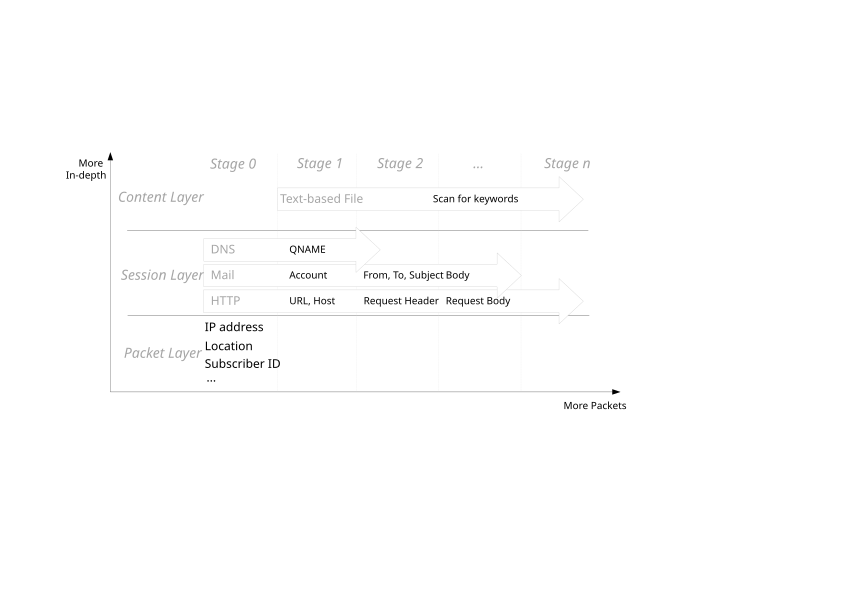
\includegraphics[width=\textwidth]{images/policy_enforcement_stage_v2.svg}
	%\caption{Figure: Inspection Stage}
	%\label{fig:system:policy_enforcement_stage_v2}
%\end{figure}

%\begin{figure}
%    \centering
%    \def\svgwidth{\columnwidth}
%    \input{../images/policy_enforcement_stage_v2.pdf_tex}
%\end{figure}

\begin{figure}[htb]
    \centering
    \includesvg{\columnwidth}{../images/policy_enforcement_stage_v2}
    %\caption{Figure}
\end{figure}


It is highly likely that even after only a relatively small number of policies have been created that there will be some that overlap 
or are subsets of the parameters that the policies use to determine which policy should be matched against the incoming traffic. 
When this happens there has to be a method to determine which policy should be applied to the packet. The method which is used by TSG is the policy hierarchy. 
In another words, policies with lower inspection layers and earlier parsing stages are precedent. For example, a HTTP session, its URL appears before response body. 
That’s why policy rules that inspect HTTP response body, are always evaluated after ones that inspect URL.


\notemark\textit{A policy rule that combines with condition fields of different layers and stages are evaluated at the last layer and stage. 
Rule stage is decided by policy condition fields; and rule modification may change the rule stages.}


As firewall maybe unable to determine the exact application from the first packet, a session may be allowed through the firewall as undecided 
until the application is identified, at which time the security rules are re-evaluated and an appropriate action is taken.


For more details about how TSG process packet flow, please see \hyperlink{link:Appendix E TSG Packet Flow}{\color{linkblue}{Appendix E TSG Packet Flow}}.

\pdfbookmark[1]{Security Policy}{Security Policy}
\section*{\hypertarget{link:Security Policy}{Security Policy}}
\label{sec:policies:security}

Security policies determine whether to deny, allow, monitor or intercept a session based on initial session attributes, 
such as the subscriber ID, IP addresses, ports, protocols and applicable protocol fields (e.g. TLS SNI). 
On TSG, security policy rules are enforced by firewall module.


All traffic passing through the firewall is matched against a session and each session is matched against a security policy rule. 
When a session match occurs, the firewall applies the matching security policy rule to bidirectional traffic in that session (client to server and server to client). 
For traffic that doesn’t match any defined rules, the default rule applies. The default rule is predefined to allow all traffic for firewall policy check. 
Although the default rule is read-only by default, you can override them and change a limited number of settings, including the tags, action (allow or deny) and log settings.


A packet is matched against the first rule that meets the defined criteria and, after a match is triggered, subsequent rules are not evaluated. 
Session that matches a rule generates a log entry at the end of the session in the security event log if you enable logging for that rule. 
The logging options are configurable for each rule.

\pdfbookmark[2]{Components of a Security Policy Rule}{Components of a Security Policy Rule}
\subsection*{\hypertarget{link:Components of a Security Policy Rule}{Components of a Security Policy Rule}}
\label{sec:policies:security:component}

The Security policy rule construct permits a combination of the required and optional fields as detailed in the following table:\\


\begin{longtable}{p{0.15\textwidth}|p{0.23\textwidth}|p{0.54\textwidth}}   
    \rowcolor{black}\multicolumn{1}{l!{\color{white}\vrule width 0.5pt}}{\textcolor{white}{\begin{tabular}{l}Required/\\Optional\end{tabular}}}  & \multicolumn{1}{l!{\color{white}\vrule width 0.5pt}}{\textcolor{white}{Field}} & \textcolor{white}{Description}\\\hline                                                                                                                                                          
    \multirow{3}{*}{Required} & Name & A label (up to 128 characters) that identifies the rule.\\ \cline{2-3}
                              & Action & Specifies an Allow, Deny, Monitor or Intercept action for the traffic based on the criteria you define in the rule. For more details, see \hyperlink{link:Security Actions}{\color{linkblue}{Security Policy Actions}}. \\ \cline{2-3}
                              & Application & The application that you wish to control. It provides application control and visibility in creating security policies that block unknown applications, while enabling, inspecting, and shaping those that are allowed. For more information, see \textbf{Objects} > \textbf{Applications} and \hyperlink{link:Appendix B Predefined Applications}{\color{linkblue}{Appendix B Predefined Application}}.\\ \hline                                                                                                        
    \multirow{9}{*}{Optional} & Source & Define host IP addresses, address groups, Subscriber ID, IP Learning, or Geographic enforcement.\\ \cline{2-3}
                              & Destination & The location or destination for the packet. Define host IP addresses, address groups, IP Learning, or Geographic enforcement.\\ \cline{2-3}
                              & Filter & All web traffics are compared against the filtering, giving you a way to safely control how your users interact with online content. You will have Filter available when you select only one of the following protocols: HTTP, SSL, DNS, MAIL, FTP and QUIC in Applicationfield.\\ \cline{2-3}
                              & Tag & A keyword or phrase that help you to identify the policy. \\ \cline{2-3}
                              & Effective Devices & Select the devices that the security rule will be applied.\\ \cline{2-3}
                              & Schedule & Schedule when (day and time) the security rule should be in effect. \\ \cline{2-3}
                              & Log Session & When enabled, traffic that match security policies will be logged in Security Event Logs. \\ \cline{2-3}
                              & Description & A text field, up to 1024 characters, used to describe the rule. \\ \cline{2-3}
                              & Enabled & Only enabled policies will be enforced.\\ \hline                                                                                                 
\end{longtable}

\pdfbookmark[2]{Actions}{Security Actions}
\subsection*{\hypertarget{link:Security Actions}{Actions}}
\label{sec:policies:security:action}

For traffic that matches the attributes defined in a security policy, you can apply the following actions:\\


\begin{longtable}{p{0.12\textwidth}|p{0.82\textwidth}}   
    \rowcolor{black}\multicolumn{1}{l!{\color{white}\vrule width 0.5pt}}{\textcolor{white}{Action}}  & \textcolor{white}{Description} \\\hline                                                                                                                                                          
    Allow &  The traffic is allowed to proceed to the next step.\\ \hline                                                                                                            
    Deny &  \begin{tabular}{l}  
            The traffic is not allowed to proceed. There are 5 Sub Action to \\
            select, they are Drop, RST (TCP reset attack), Block, Alert and \\
            Redirect.\\
            Sub Action of Deny:\\
            \textbf{Drop}, silently drops the traffic.\\
            \textbf{RST}, sends a TCP reset to the client-side device.\\
            \textbf{Block}, sends 403/404 return code and customized content to \\
            the client.\\
            \textbf{Alert}, sends 200/204 return code and customized content to the \\
            client.\\
            \textbf{Redirect}, redirects to the link set in the policy configuration.
            \end{tabular}\\ \hline                                                                                                          
    Intercept & Intercept HTTP/HTTPS traffic for proxy. If the traffic use SSL/TLS, it will be decrypted.\\\hline 
    Monitor &  Scan all allowed traffic and generate a detailed log.\\\hline 
\end{longtable}

\pdfbookmark[2]{Applications and Filters}{Security Applications and Filters}
\subsection*{\hypertarget{link:Security Applications and Filters}{Applications and Filters}}
\label{sec:policies:security:filter}

AppSketch is a traffic classification system available in TSG firewalls, determines what an application is irrespective of port, protocol, 
encryption or any other evasive tactic used by the application. It applies multiple classification mechanisms, (including application signatures, 
application protocol decoding, heuristics, and machine learning) to your network traffic stream to accurately identify applications.


Applications enables visibility into the applications on the network, so you can learn how they work and understand their behavioral characteristics 
and their relative risk. When you define policy rules to control traffic, applications begin to classify traffic without any additional configuration.


\begin{longtable}{p{0.14\textwidth}|p{0.19\textwidth}|p{0.58\textwidth}}   
    \rowcolor{black}\multicolumn{2}{l!{\color{white}\vrule width 0.5pt}}{\textcolor{white}{Applications Type}}  & \textcolor{white}{Description}\\\hline                                                                                                                                                          
    \multirow{3}{*}{Application} & Basic Protocols & Network protocols ensure that computer network devices can transmit and receive data using a common language regardless of their different designs, hardware or infrastructures. 
    List all 50 basic protocols: 
    
    
    Unknown\_TCP, Unknown\_UDP, Unknown\_Other, DNS, FTP, FTPS, HTTP, HTTPS, ICMP, IKE, IMAP, MAIL, IMAPS, IPSEC, XMPP, L2TP, NTP, POP3, POP3S, PPTP, QUIC, SIP, SMB, SMTP, SMTPS, SPDY, SSH, SSL, SOCKS, TELNET, DHCP, RADIUS, OPENVPN, STUN, TEREDO, DTLS, DoH, ISAKMP, MDNS, NETBIOS, NETFLOW, RDP, RTCP, RTP, SLP, SNMP, SSDP, TFTP, BJNP, LDAP, RTMP, RTSP. 
    \\ \cline{2-3}
                                 & \tabincell{l}{Predefined\\ Applications} & TSG has various predefined applications. \\ \cline{2-3}
                                 & \tabincell{l}{Customized\\ Applications} & TSG allows you create custom applications and reference the customized application objects in policy.\\\hline
    Selector & Selector & TSG allows you dynamically group applications based on application properties that you define into one object Selector. It is available for Action Allow and Deny. For more details, see \hyperlink{link:Application Selector}{\color{linkblue}{Application Selector}}.    \\ \hline 
    Group & Group & An application group is an object that contains applications that you want to treat similarly in a policy. It is available for Action Allow and Deny. For more details, see \hyperlink{link:Application Group}{\color{linkblue}{Application Group}}.    \\ \hline                                                                                                 
\end{longtable}


You will have Filter available when you select only one of the following protocols: HTTP, SSL, DNS, MAIL, FTP and QUIC. 
The following table lists different Filter fields for each protocol and the available object type you can select for each filter field, 
it also shows whether each filter field support allow, deny, monitor and intercept action or not. 


%
    %\rowcolor{black}\multirow{2}{*}{\multicolumn{1}{@{}l!{\color{white}\vrule width 0.5pt}}{\textcolor{white}{Protocol}}}  & \multirow{2}{*}{\multicolumn{1}{@{}l!{\color{white}\vrule width 0.5pt}}{\textcolor{white}{Filter Field}}} & 
    %\multirow{2}{*}{\multicolumn{1}{@{}l!{\color{white}\vrule width 0.5pt}}{\textcolor{white}{Available Object}}} & \multicolumn{4}{@{}l}{\textcolor{white}{Applicable Actions}} 
    %&\textcolor{white}{Applicable Actions} &\textcolor{white}{Applicable Actions} &\textcolor{white}{Applicable Actions}
    %\multicolumn{1 !{\color{white}\vrule width 0.5pt}}{\textcolor{white}{Protocol}}   
    %\textcolor{white}{Protocol}
    %!{\color{white}\vrule width 0.5pt}
%\begin{longtable}{p{0.16\textwidth}|p{0.17\textwidth}|p{0.18\textwidth}|p{0.1\textwidth}|p{0.1\textwidth}|p{0.11\textwidth}|p{0.12\textwidth}}
    %\setlength{\arrayrulewidth}{2pt}
\begin{longtable}{p{0.13\textwidth}|p{0.15\textwidth}|p{0.14\textwidth}|p{0.07\textwidth}|p{0.07\textwidth}|p{0.11\textwidth}|p{0.11\textwidth}} 
    \rowcolor{black}
    \multicolumn{1}{l !{\vlinewhite}}{} &
    \multicolumn{1}{l !{\vlinewhite}}{}  & 
    \multicolumn{1}{l !{\vlinewhite}}{} & 
    \multicolumn{4}{c}{\textcolor{white}{Applicable Actions}} \\ 
    \arrayrulecolor{white}\cline{4-7}  
    \rowcolor{black}
    \multicolumn{1}{l !{\vlinewhite}}{\multirow{-2}{*}{\textcolor{white}{Protocol}}} & 
    \multicolumn{1}{l !{\vlinewhite}}{\multirow{-2}{*}{\textcolor{white}{Filter Field}}} &
    \multicolumn{1}{l !{\vlinewhite}}{\multirow{-2}{*}{\textcolor{white}{\tabincell{l}{Available\\ Object}}}} & 
    \multicolumn{1}{l!{\color{white}\vrule width 0.5pt}}{\textcolor{white}{Allow}}  & 
    \multicolumn{1}{l!{\color{white}\vrule width 0.5pt}}{\textcolor{white}{Deny}}  & 
    \multicolumn{1}{l!{\color{white}\vrule width 0.5pt}}{\textcolor{white}{Monitor}} & 
    \textcolor{white}{Intercept} \\ \arrayrulecolor{black}\hline                                                                                                                                                          
    \multirow{6}{*}{HTTP} & Host & \tabincell{l}{FQDNs\\ Category} & \cmark & \cmark & \cmark & \cmark\\ \cline{2-7}
                          & URL & URLs & \cmark & \cmark & \cmark & \xmark \\ \cline{2-7}
                          & \tabincell{l}{Request\\ Header} & \multirow{2}{*}{\tabincell{l}{HTTP\\ Signatures}} & \xmark & \cmark & \cmark & \xmark\\ \cline{2-2}\cline{4-7}
                          & \tabincell{l}{Response\\ Header} &  & \xmark & \cmark & \cmark & \xmark\\ \cline{2-7}
                          & \tabincell{l}{Request\\ Content} & \multirow{2}{*}{Keywords} & \xmark & \cmark & \cmark & \xmark\\ \cline{2-2}\cline{4-7}
                          & \tabincell{l}{Response\\ Content}  &  & \xmark &  \cmark & \cmark & \xmark\\\hline
    \multirow{3}{*}{SSL} & SNI & \multirow{3}{*}{\tabincell{l}{FQDNs\\ Category}} & \cmark & \cmark & \cmark & \cmark   \\ \cline{2-2}\cline{4-7}
                         & CN &  & \xmark & \cmark & \cmark & \xmark   \\ \cline{2-2}\cline{4-7}
                         & SAN &  & \xmark & \cmark & \cmark & \xmark   \\ \hline   
    QUIC & SNI & \tabincell{l}{FQDNs\\ Category} & \cmark & \cmark & \cmark & \xmark   \\ \hline 
    DNS & QNAME & \tabincell{l}{FQDNs\\ Category} & \xmark & \cmark & \cmark & \xmark   \\ \hline 
    \multirow{7}{*}{MAIL}  & Account & \multirow{3}{*}{\tabincell{l}{Accounts}} & \xmark & \cmark & \cmark & \xmark   \\ \cline{2-2}\cline{4-7} 
                           & From &  & \xmark & \cmark & \cmark & \xmark   \\ \cline{2-2}\cline{4-7}
                           & To &  & \xmark & \cmark & \cmark & \xmark   \\ \cline{2-7}
                           & Subject & \multirow{4}{*}{\tabincell{l}{Keywords}} & \xmark & \cmark & \cmark & \xmark   \\ \cline{2-2}\cline{4-7}
                           & Content &  & \xmark & \cmark & \cmark & \xmark   \\ \cline{2-2}\cline{4-7}
                           & \tabincell{l}{Attachment\\ Name} &  & \xmark & \cmark & \cmark & \xmark   \\ \cline{2-2}\cline{4-7}
                           & \tabincell{l}{Attachment\\ Content} &  & \xmark & \cmark & \cmark & \xmark   \\ \hline 
    \multirow{3}{*}{FTP} & URI & URLs & \xmark & \cmark & \cmark & \xmark   \\ \cline{2-7}
                         & Content & Keywords & \xmark & \cmark & \cmark & \xmark   \\ \cline{2-7}
                         & Account & Accounts & \xmark & \cmark & \cmark & \xmark   \\ \hline
\end{longtable}


The Evaluation Order for security policy is described as following. 


Security policy is evaluated before Proxy policy. Proxy manipulation requires targeted sessions are intercepted in security policies. 
That is to say an intercept security policy rule is the prerequisite for proxy policy. 


Traffic can match one or multiple security policy rules with monitor action. This means traffic can hit multiple security policy rules only with monitor actions. 
For security policies with allow, deny and intercept actions, traffic can only hit one policy that meets the defined criteria with top priority. 
After a match is triggered, subsequent rules are not evaluated. It is important to know the policy evaluation order to create policies accordingly. 


There are three factors in evaluation of policies. They are condition, action and policy ID in sequence.


\begin{description}[leftmargin=0pt,itemindent=0em,itemsep=0.5ex]
    \item
    \begin{enumerate}
        %\setlength{\itemindent}{-30pt}%
        \setlength{\topsep}{0pt} %列表到上下文的垂直距离
        %\setlength{\itemsep}{-10pt} %条目间距
        \item The ranked evaluation order for condition is:\\
        IP > FQDN/URL/Request Header > Request Content > Response Header >Response Content
        \item The priority queue of action is:\\
        Allow > Deny > Intercept > Monitor\\
        For policies that match \hyperlink{link:SSL Decryption Exclusion}{\color{linkblue}{SSL Decryption Exclusion}} are evaluated before intercept policies.
        \item Prioritize policies in descending order by policy ID. 
    \end{enumerate}
\end{description}


For more details about how TSG process packet flow, please see \textbf{\hyperlink{link:Appendix E TSG Packet Flow}{\color{linkblue}{Appendix E TSG Packet Flow}}}.

\pdfbookmark[2]{Allow Rules}{Allow Rules}
\subsection*{\hypertarget{link:Allow Rules}{Allow Rules}}
\label{sec:policies:security:allow}

TSG allows the network traffic to pass through, without apply further policy checking. You can define traffic that you choose not to enforce policies because of business, 
regulatory, personal, or other reasons, such as financial, health, military, or government traffic. 


Generally, allow policies need not generate logs. However, if you enable Log Session, traffic that matches the allow policy rule will also be logged in Event Logs. 
If you wish to have logs, it is recommended to create monitor rules with Log Session enabled, which will have the same effect.

\pdfbookmark[2]{Intercept Rules}{Intercept Rules}
\subsection*{\hypertarget{link:Intercept Rules}{Intercept Rules}}
\label{sec:policies:security:intercept}

Security policy with intercept action allows you to define traffic that you want the Proxy to terminate. Both HTTP and HTTPS sessions could be terminated. 
You can do further manipulation on intercepted traffic with Proxy Policy. 


When an SSL session is set to intercept, the Proxy terminates the client-side session and initiates a new server-side session. 
Thus, the server certificate is replaced and content is decrypted. 


You can specify different keyrings for individual intercept policy. If not, the Proxy uses the default keyring for trusted website. 
Keyrings are managed via \textbf{Certificate Managements} > \textbf{\hyperlink{link:Decryption Keyrings}{\color{linkblue}{Decryption Keyrings}}}.

\pdfbookmark[3]{Intercept Options}{Intercept Options}
\subsubsection*{\hypertarget{link:Intercept Options}{Intercept Options}}
\label{sec:policies:security:intercept:option}

While policy objects enable you to identify traffic to enforce policies, policy profiles help you define further action. 
When you create an Intercept policy and select the SSL application to enable access to encrypted sites, you will have three Action Parameters, 
namely Keyring, Mirror Decrypted Traffic and Decryption Profile. They serve as your intercept options. 


• You can specify a Keyring or use TrustedDefault. To specify a different Keyring, select the item from drop-down or click the plus icon to create a new one. For more details, see \hyperlink{link:Decryption Keyrings}{\color{linkblue}{Decryption Keyrings}}. 


• If you enable Mirror Decrypted Traffic, you can select one item from drop-down or click the plus icon to create a new profile. For more details, see \hyperlink{link:Traffic Mirror Profile}{\color{linkblue}{Traffic Mirror Profile}}.


• You can use decryption-default for your Decryption Profile, or you can select different one from drop-down and create new ones. For more details, see \hyperlink{link:Decryption Profile}{\color{linkblue}{Decryption Profile}}.

\pdfbookmark[3]{Proxy Limitations}{Proxy Limitations}
\subsubsection*{\hypertarget{link:Proxy Limitations}{Proxy Limitations}}
\label{sec:policies:security:intercept:limitation}

There are two types of traffic that exclude from decryption. They are the proxy limitations. One is that you choose not to decrypt because of business, regulatory, 
personal, or other reasons. The other is traffic that breaks decryption for technical reasons:


\begin{itemize}
    \item Asymmetric Routing Traffic 
    \item Certificate Pinning Apps:
    \begin{itemize}
        \item[-] Facebook, Instagram
        \item[-] YouTube, Gmail, Google Search
        \item[-] Twitter
        \item[-] Apple Store   
    \end{itemize} 
    \item Mutual Authentication (Client Certificate Request) 
    \item Some android System that unable to install root certificate
    \item Website using HPKP
    \item Nonstandard SSL/TLS implications
    \item SSLv1.0, SSLv2.0 are not supported
    \item Unsupported ciphers          
\end{itemize}
For more details, see \hyperlink{link:SSL Decryption Exclulsion}{\color{linkblue}{SSL Decryption Exclulsion}}.


If you wish to exclude FQDN from decryption, create an SSL Decryption Exclusion item and it will immediately become effective. 
For policies that match SSL Decryption Exclusion are evaluated before intercept policies.

\pdfbookmark[3]{Intercept Trouble Shooting}{Intercept Trouble Shooting}
\subsubsection*{\hypertarget{link:Intercept Trouble Shooting}{Intercept Trouble Shooting}}
\label{sec:policies:security:intercept:troubleshooting}

You can find out if the interception is successful by checking if the certificates are issued by your pre-configured Root CA. 
You should exercise with cautions because web applications may not cooperate with SSL interception.


• Your connection is not private/secure


Visit the website that should match the intercept rule. For Chrome, Microsoft Internet Explorer and Firefox, click the lock icon next to the address bar to view website certificates. 
If the browser warning that the connection is not secure, one possible reason is you haven’t install/trust the root certificate yet. 


Another possible reason is that the site uses an incomplete certificate chain, the Proxy doesn’t automatically fix the chain as a browser would. 
Although Proxy is able to cache unseen intermediate certificates that issued 
by trusted root (\textbf{Certificate Managements} > \textbf{\hyperlink{link:Cached Intermediate Certificates}{\color{linkblue}{Cached Intermediate Certificates}}}), 
you still need to manually download the missing intermediate certificates occasionally. 
Missing certificates could be import via \textbf{Certificate Managements} > \textbf{\hyperlink{link:Trusted Certificate Authorities}{\color{linkblue}{Trusted Certificate Authorities}}}.


• Handling Web Sites Where Decrypt Re-sign Works for a Browser but not an App (SSL or Certificate Authority Pinning)


Some apps for smart phones and other devices use a technique called SSL (or Certificate Authority) pinning. 
The SSL pinning technique embeds the hash of the original server certificate inside the app itself. 
As a result, when the app receives the resigned certificate from TSG, the hash validation fails and the connection is aborted. 


If internet users cannot connect to the web site using the site’s app, but they can connect using the web browser, 
even when using the browser on the same device where the app fails. For example, users cannot use the Facebook iOS or android app, 
but they can point Safari or Chrome at https://www.facebook.com and make a successful connection. 


Because SSL pinning is specifically used to avoid man-in-the-middle attacks, there is no workaround. You must choose between the following options:


- Support app users, by enabling Certificate Pinning dynamic bypass option, in which case you can only decrypt browser traffic to the site. 
For more details, see \textbf{Proxy Profiles} > \textbf{\hyperlink{link:Trusted Certificate Authorities}{\color{linkblue}{Decryption Profile}}}.


- Force users to use browsers only. If you must decrypt traffic to the site, you will need to inform users that they cannot use the site’s app 
when connecting through your network, that they must use their browsers only.

\pdfbookmark[2]{Create a Security Policy Rule}{Create a Security Policy Rule}
\subsection*{\hypertarget{link:Create a Security Policy Rule}{Create a Security Policy Rule}}
\label{sec:policies:security:create}

\begin{description}
    \item[STEP 1.]	Add a rule. Select \textbf{Policies} > \textbf{Security} and click \textbf{Create} to add a new rule. Enter a descriptive \textbf{Name} for the rule.
    \item[STEP 2.]	Define what action you want TSG to take for traffic that matches the rule. Select an \textbf{Action}. 
    See \hyperlink{link:Security Actions}{\color{linkblue}{Security Policy Actions}} for a description of each action.
    \item[STEP 3.]	Define the matching criteria for the source fields in the packet. Specify single or multiple \textbf{Source} IP Addresses/ Subscriber IDs or leave the value set to any. If you don’t add entries to the list, the policy has no IP address restrictions.
    \item[STEP 4.]	Define the matching criteria for the destination fields in the packet. Specify one or multiple \textbf{Destination} IP Addresses or leave the value set to any.
    
    
    \notemark\textit{As a best practice, use address objects as the Destination Address to enable access to only specific servers or specific groups of servers especially 
    for commonly exploited services, such as DNS and VPN.}
    \item[STEP 5.]	Select one or more \textbf{Applications}. There are built-in protocols and well-known Applications and customized Applications in the list. 
    You can search the application you want to fill in. You can also use application \textbf{Selector} and \textbf{Group} as objects in policy. 
    For more details, see \textbf{Security Policy} > \textbf{\hyperlink{link:Security Applications and Filters}{\color{linkblue}{Applications and Filters}}} and \textbf{Objects} > \textbf{\hyperlink{link:Applications}{\color{linkblue}{Applications}}}.
    \item[STEP 6.]	(\textcolor{gold}{Optional}) Specify a \textbf{Filter} as match criteria for the rule. For example, select a \textbf{Category} for \textbf{Host}. 
    If you select a category, only web traffic will match the rule and only if the traffic is destined for that specified category. 
    For more details, see \textbf{Security Policy} > \textbf{\hyperlink{link:Security Applications and Filters}{\color{linkblue}{Applications and Filters}}}.
    
    
    \notemark\textit{Filter is not available when multiple or no applications are selected.}
    \item[STEP 7.]	(\textcolor{gold}{Optional})Specify a \textbf{Tag} or leave the value empty.
    You can select one or more Policy Tags which are created from \textbf{Policies} > \textbf{Tags} previously. 
    Optionally, you can click the plus icon to create new Tags. After you click the icon, a page will slide in on the right. Enter the \textbf{Tag Category}. 
    Pick a \textbf{Color}. And add one or multiple \textbf{Tags}. Then you can select the tag you just created from the list.
    \item[STEP 8.]	Specify \textbf{Effective Devices} by choosing Device Tags or leave the value empty, which means the policy is effective on all devices by default. 
    Device Tags are built-in labels to classify the devices according to user’s requirement when TSG is deployed. Normally, the Device Tags will be classified by areas or ISPs.
    \item[STEP 9.]	(\textcolor{gold}{Optional})Enter a \textbf{Description} for the rule.
    \item[STEP 10.]	(\textcolor{gold}{Optional})Select a \textbf{Schedule} or leave the value set to always. For more details, see \textbf{Policies} > \textbf{\hyperlink{link:Schedules}{\color{linkblue}{Schedules}}}.
    
    
    \notemark\textit{If you select a schedule, the schedule will determine when the policy will be enabled and effective. 
    This means you don’t have to turn the Enabled switch on. Because the policy will automatically be effective according to your specified schedule. 
    And even if you set the policy Enabled, the policy will not be effective, if it has not reached the schedule time frame.}
    \item[STEP 11.]	Verify that \textbf{Log Session} is enabled if you wish to have logs. Only traffic that matches a Security policy rule will be logged. 
    \item[STEP 12.]	Verify that \textbf{Enabled} is enabled.
    \item[STEP 13.]	Click \textbf{OK} to save the policy rule.
    \item[STEP 14.]	(\textcolor{gold}{Optional})To verify that you have set up your policies effectively, test whether your Security policy rules are being evaluated and determine which Security policy rule applies to a traffic flow. For example, to verify the policy rule that will be applied for a client with the IP address 192.168.0.1 when it sends a HTTP request to the 172.16.0.1 server:
    \begin{enumerate} 
        \item Select \textbf{Settings} > \textbf{Trouble Shooting} and select \textbf{Policy Verify} tab.
        \item Select \textbf{Security Policy Match} from the \textbf{Select Test} drop-down. 
        \item Enter the \textbf{Client IP} and \textbf{Server IP} addresses or leave it set to default.
        \item Specify the \textbf{Client Port} and \textbf{Server Port} or leave it set to default.
        \item Select the \textbf{Protocol} and \textbf{APP ID}. 
        \item Click \textbf{Verify} to execute the \textbf{Security policy match} test.
    \end{enumerate}
    \item[STEP 15.]	After the policy has been hit. View \textbf{Logs} to monitor the policy rule status and determine the effectiveness of the policy rule. 
    Select \textbf{Logs} > \textbf{Security Event Logs} and view relative information about the policy.
\end{description}

You can view detailed information about the policy you just created. To edit and delete the policy, find the item you want to edit or delete in the list. Click \textbf{Edit} or \textbf{Delete} at the top left.


You can export the contents of policies to a json file. First, search policies according to ID, Name. Then, click the Export icon on the right to download and save the file to your local folder.


You can also import policies by clicking the import icon. Only json and txt formats can be uploaded. You can take the exported file as template for import.


Select the checkbox for policies in the list and Click \textbf{Watch} at the bottom to add to Watch List. And then you can click the star icon in the bottom right and select Policy tab to view the Watch List. 
You can search policies by ID and Name in the list. The Watch feature gives you the ability to observe policies and objects on which you wish to keep an eye any time. 


\notemark\textit{Policy No. 0: For traffic that passes through TSG but does not hit any policies, the traffic is executed according to policy No. 0. 
The conditions of policy No. 0 are all any, and by default the action is Allow. Policy No. 0 is forbidden to edit.}

\pdfbookmark[1]{Proxy Policy}{Proxy Policy}
\section*{\hypertarget{link:Proxy Policy}{Proxy Policy}}
\label{sec:policies:proxy}

Proxy policy instructs the proxy how to manipulate a session. Manipulation requires targeted sessions are intercepted in security policies. An individual manipulation policy rules determine whether to allow, monitor, deny or manipulate a session based on traffic attributes. Valid objects depend on specific action.


Proxy policy works correctly on all platforms, including Windows, Linux, MacOS, Android, iOS, etc. and also supports console commands, such as wget and curl, mobile devices, tablets and workstations in all locations. But TSG does not support TV device that cannot install the certificate, and device with Android 7.0 and versions below. 


For the site which breaks decryption for certificate pinning, the proxy only can bypass or deny the traffic based on your configuration. For more details, see \hyperlink{link:Decryption}{\color{linkblue}{Decryption}}.

\pdfbookmark[2]{Components of a Proxy Policy Rule}{Components of a Proxy Policy Rule}
\subsection*{\hypertarget{link:Components of a Proxy Policy Rule}{Components of a Proxy Policy Rule}}
\label{sec:policies:proxy:component}

The Proxy Policy rule construct permits a combination of the required and optional fields as detailed in the following table:


\begin{longtable}{p{0.15\textwidth}|p{0.23\textwidth}|p{0.54\textwidth}}   
    \rowcolor{black}\multicolumn{1}{l!{\color{white}\vrule width 0.5pt}}{\textcolor{white}{\begin{tabular}{l}Required/\\Optional\end{tabular}}}  & \multicolumn{1}{l!{\color{white}\vrule width 0.5pt}}{\textcolor{white}{Field}} & \textcolor{white}{Description}\\\hline                                                                                                                                                          
    \multirow{2}{*}{Required} & Name & A label (up to 128 characters) that identifies the rule.\\ \cline{2-3}
                              & Action & Specifies an Allow, Deny, Monitor, Redirect, Replace, Hijack or Insert action for the traffic based on the criteria you define in the rule. 
                              For more details, see \hyperlink{link:Proxy Actions}{\color{linkblue}{Proxy Policy Actions}}. \\ \hline
    \multirow{11}{*}{Optional} & Source & Define host IP addresses, address groups, Subscriber ID, IP Learning, or Geographic enforcement.\\ \cline{2-3}
                              & Destination & The location or destination for the packet. Define host IP addresses, address groups, IP Learning, or Geographic enforcement.\\ \cline{2-3}
                              & Filter & All web traffics are compared against the filtering, giving you a way to safely control how your users interact with online content. You must fill one of the Source, Destination or Filter.\\ \cline{2-3}
                              & Application & The application that you wish to control. It provides application control and visibility in creating proxy policies that block unknown applications, while enabling, inspecting, and shaping those that are allowed.\\ \cline{2-3}                                                                                                      
                              & Tag & A keyword or phrase that help you to identify the policy. \\ \cline{2-3}
                              & Effective Devices & Select the devices that the security rule will be applied.\\ \cline{2-3}
                              & Schedule & Schedule when (day and time) the security rule should be in effect. \\ \cline{2-3}
                              & Log Session & When enabled, traffic that match security policies will be logged in Security Event Logs. \\ \cline{2-3}
                              & Log Option &  Metadata and All: Metadata only structured logs are recorded. All provides raw log files for some special log fields, such as content of HTTP request header or HTTP response content.\\ \cline{2-3}
                              & Description & A text field, up to 1024 characters, used to describe the rule. \\ \cline{2-3}
                              & Enabled & Only enabled policies will be enforced.\\ \hline                                                                                                 
\end{longtable}

\pdfbookmark[2]{Actions}{Proxy Actions}
\subsection*{\hypertarget{link:Proxy Actions}{Actions}}
\label{sec:policies:proxy:action}

For traffic that matches the attributes defined in a proxy policy, you can apply the following actions: 


\begin{longtable}{p{0.12\textwidth}|p{0.82\textwidth}}   
    \rowcolor{black}\multicolumn{1}{l!{\color{white}\vrule width 0.5pt}}{\textcolor{white}{Action}}  & \textcolor{white}{Description} \\\hline                                                                                                                                                          
    Allow & The Proxy pass-through the matched sessions. The traffic is allowed to proceed to the next step.\\ \hline                                                                                                            
    Deny & The Proxy terminate matched HTTP session with an error page. More information of uploading a html file, see \textbf{Proxy Profile} > \textbf{\hyperlink{link:Response Pages}{\color{linkblue}{Response Pages}}}.\\ \hline                                                                                                           
    Monitor &  The Proxy produce a log to record matched HTTP session information.\\\hline 
    Redirect &  The Proxy redirect matched HTTP session to a predefined URL. Since redirection
                need to be performed before delivering response to client, condition of response body is not
                applicable in this action. You MUST configure the redirect response via Response Code and Redirect
                URL. The Destination URL should begin with a valid protocol (http:|https:). You SHOULD NOT select
                301 as Response Code unless you exactly know what you are doing. This action produces a log. \\ \hline 
    Replace &  The Proxy Searches in a given HTTP part to Find a given string, and Replace any matches with another given string. If no match was found, the session remained untouched. For performance concerns, condition of request body and response body is not available in this action. For example, you can configure the Proxy to search in the response body of URL “www.example.com/index.html”, find every “string1” and replace with “string2”. This action produces a log. You can use regex to do replacement, e.g. case insensitive find “(?i)CaSEInSensitive(?-i)”. You can add multiple replacement.


    \notemark \textit{Note that when searching and replacing content, there must be at least 512 characters of the replaced content. And the system support utf8 encoding and has the ability to replace content of different languages, including Kazakh, Russian and English.}\\ \hline 
    Hijack & The Proxy hijack a downloading file. Supported file type are img, exe, apk and html. More information of uploading a file for hijack, see \textbf{Proxy Profile} > \textbf{\hyperlink{link:Hijack Files}{\color{linkblue}{Hijack Files}}}.\\ \hline 
    Insert & The Proxy insert a “js” or “css” scripts to webpages. More details of uploading a script, see \textbf{Proxy Profile} > \textbf{\hyperlink{link:Insert Scripts}{\color{linkblue}{Insert Scripts}}}.\\ \hline           
\end{longtable}

\pdfbookmark[2]{Applications and Filters}{Proxy Applications and Filters}
\subsection*{\hypertarget{link:Proxy Applications and Filters}{Applications and Filters}}
\label{sec:policies:proxy:filter}

Only two basic protocol HTTP and DoH are available for the Application in proxy policy. The following table lists different Filter fields for the two protocols and the available object type you can select for each filter field, it also shows whether each filter field support allow, deny, monitor, redirect, replace, hijack and insert action or not. 


Only two basic protocol HTTP and DoH are available for the Application in proxy policy. The following table lists different Filter fields for the two protocols and the available object type you can select for each filter field, it also shows whether each filter field support allow, deny, monitor, redirect, replace, hijack and insert action or not. 


\begin{longtable}{p{0.12\textwidth}|p{0.02\textwidth}|p{0.02\textwidth}|p{0.02\textwidth}|p{0.02\textwidth}|p{0.03\textwidth}|p{0.03\textwidth}|p{0.04\textwidth}|p{0.04\textwidth}|p{0.04\textwidth}|p{0.04\textwidth}|p{0.03\textwidth}|p{0.03\textwidth}|p{0.03\textwidth}|p{0.03\textwidth}}
    \rowcolor{black}
    \multicolumn{1}{l !{\vlinewhite}}{} &
    \multicolumn{14}{c}{\textcolor{white}{\tabincell{l}{Filter Fields Fit in Actions\\ \qquad HTTP | DoH }}} \\ \arrayrulecolor{white}\cline{2-15} 
    \rowcolor{black}
    \multicolumn{1}{l !{\vlinewhite}}{\multirow{-2}{*}{\textcolor{white}{Filter Type}}}&
    \multicolumn{2}{l!{\color{white}\vrule width 0.5pt}}{\textcolor{white}{Allow}}  & 
    \multicolumn{2}{l!{\color{white}\vrule width 0.5pt}}{\textcolor{white}{Deny}}  & 
    \multicolumn{2}{l!{\color{white}\vrule width 0.5pt}}{\textcolor{white}{Monitor}} & 
    \multicolumn{2}{l!{\color{white}\vrule width 0.5pt}}{\textcolor{white}{Redirect}} & 
    \multicolumn{2}{l!{\color{white}\vrule width 0.5pt}}{\textcolor{white}{Replace}} & 
    \multicolumn{2}{l!{\color{white}\vrule width 0.5pt}}{\textcolor{white}{Hijack}} & 
    \multicolumn{2}{l}{\textcolor{white}{Insert}} \\\arrayrulecolor{black}\hline                                                                                                                                                           
    Host & \cmark & \xmark & \cmark & \xmark & \cmark & \xmark & \cmark & \cmark & \cmark & \xmark & \cmark & \xmark & \cmark & \xmark  \\ \hline 
    URL & \cmark & \xmark & \cmark & \xmark & \cmark & \xmark & \cmark & \xmark & \cmark & \xmark & \cmark & \xmark & \cmark & \xmark  \\ \hline 
    \tabincell{l}{Request\\ Header} & \cmark & \xmark & \cmark & \xmark & \cmark & \xmark & \cmark & \xmark & \cmark & \xmark & \cmark & \xmark & \cmark & \xmark  \\ \hline 
    \tabincell{l}{Response\\ Header} & \cmark & \xmark & \cmark & \xmark & \cmark & \xmark & \cmark & \xmark & \cmark & \xmark & \cmark & \xmark & \cmark & \xmark  \\ \hline 
    \tabincell{l}{Request\\ Content} & \xmark & \xmark & \cmark & \xmark & \cmark & \xmark & \cmark & \xmark & \xmark & \xmark & \xmark & \xmark & \xmark & \xmark  \\ \hline
    \tabincell{l}{Response\\ Content} & \xmark & \xmark & \cmark & \xmark & \cmark & \xmark & \xmark & \xmark & \xmark & \xmark & \xmark & \xmark & \xmark & \xmark  \\ \hline 
    QNAME & \xmark & \xmark & \xmark & \xmark & \xmark & \xmark & \xmark & \cmark & \xmark & \xmark & \xmark & \xmark & \xmark & \xmark  \\ \hline                           
\end{longtable}
Object type available for Filter:


\begin{longtable}{p{0.25\textwidth}|p{0.05\textwidth}|p{0.09\textwidth}|p{0.04\textwidth}|p{0.14\textwidth}|p{0.07\textwidth}}
    %\rowcolor{black}
    \multicolumn{1}{l !{\vlinewhite}}{\cellcolor{black}} &
    \multicolumn{5}{c}{\textcolor{white}{\cellcolor{black}Object Type}} \\ \arrayrulecolor{white}\cline{2-6} 
    %\rowcolor{black}
    \multicolumn{1}{l !{\vlinewhite}}{\multirow{-2}{*}{\cellcolor{black}\textcolor{white}{Filter Type}}} & 
    \multicolumn{1}{l!{\vlinewhite}}{\textcolor{white}{\cellcolor{black}FQDN}}  & 
    \multicolumn{1}{l!{\vlinewhite}}{\textcolor{white}{\cellcolor{black}Category}}  & 
    \multicolumn{1}{l!{\vlinewhite}}{\textcolor{white}{\cellcolor{black}URL}} & 
    \multicolumn{1}{l!{\vlinewhite}}{\textcolor{white}{\cellcolor{black}HTTP Signature}} & 
    \multicolumn{1}{l}{\textcolor{white}{\cellcolor{black}Keyword}} \\\arrayrulecolor{black}\hline                                                                                                                                                           
    Host & \cmark & \cmark & & &  \\ \hline 
    URL &  &  & \cmark & &  \\ \hline 
    Request Header &  & & & \cmark &  \\ \hline 
    Response Header &  & & & \cmark &  \\ \hline 
    Request Content &  & & & & \cmark \\ \hline 
    Response Content &  & & & & \cmark \\ \hline 
    QNAME & \cmark & \cmark & & &  \\ \hline                        
\end{longtable}

The Evaluation Order for proxy policy is described as following. 


Security policy is evaluated in preference to Proxy policy. Proxy manipulation requires targeted sessions are intercepted in security policies. That is to say an intercept security policy is the prerequisite for proxy policy.


For proxy policies with allow action, traffic can only hit one policy that meets the defined criteria. After a match is triggered, subsequent rules are not evaluated. Except allow action, proxy policies with other actions can be matched together only with monitor policies. This means traffic can hit a block proxy policy and a monitor proxy policy that meets the defined criteria at the same time. It is important to know the policy evaluation order to create policies accordingly.


There are three factors in evaluation of policies. They are condition, action and policy ID in sequence. 


\begin{description}[leftmargin=0pt]
    \item
    \begin{enumerate}
        \setlength{\topsep}{0pt} %列表到上下文的垂直距离
        %\setlength{\itemsep}{0.3ex}
        \item The ranked evaluation order for condition is:\\
        IP > FQDN/URL/Request Header > Request Content > Response Header >Response Content
        \item The priority queue of action is:\\
        Allow > Block (Monitor) >Redirect (Monitor)> Replace (Monitor) > Hijack (Monitor) > Insert (Monitor) 
        \item Prioritize policies in descending order by policy ID.
    \end{enumerate}
\end{description}


For more details about how TSG process packet flow, please see \textbf{\hyperlink{link:Appendix E TSG Packet Flow}{\color{linkblue}{Appendix E TSG Packet Flow}}}.

\pdfbookmark[2]{Create a Proxy Policy Rule}{Create a Proxy Policy Rule}
\subsection*{\hypertarget{link:Create a Proxy Policy Rule}{Create a Proxy Policy Rule}}
\label{sec:policies:proxy:create}

\begin{description}
    \item[STEP 1.]	Add a rule. Select \textbf{Policies} > \textbf{Proxy} and click \textbf{Create} to add a new rule. Enter a descriptive \textbf{Name} for the rule.
    \item[STEP 2.]	Define what action you want TSG to take for traffic that matches the rule. Select an \textbf{Action}. See \hyperlink{link:Proxy Actions}{\color{linkblue}{Proxy Policy Actions}} for a description of each action.
    \item[STEP 3.]	Define the matching criteria for the source fields in the packet. Specify one or multiple \textbf{Source} IP Addresses/ Subscriber IDs or leave the value set to any. If you don’t add entries to the list, the policy has no IP address restrictions.
    \item[STEP 4.]	Define the matching criteria for the destination fields in the packet. Specify single or multiple \textbf{Destination} IP Addresses or leave the value set to any.


    \notemark\textit{As a best practice, use address objects as the Destination Address to enable access to only specific servers or specific groups of servers especially for commonly exploited services, such as DNS and VPN.}
    \item[STEP 5.]	(\textcolor{gold}{Optional})If the Action is Redirect, specify the \textbf{Application}.
    \item[STEP 6.]	(\textcolor{gold}{Optional}) Specify \textbf{Filters} as match criteria for the rule. For example, select a \textbf{Category} for \textbf{Host}. 
    If you select a category, only web traffic will match the rule and only if the traffic is destined for that specified category. 
    For more details, see \textbf{Proxy Policy} > \textbf{\hyperlink{link:Proxy Applications and Filters}{\color{linkblue}{Applications and Filters}}} and \textbf{Objects} > \textbf{\hyperlink{link:Applications}{\color{linkblue}{Applications}}}.
    \item[STEP 7.]	(\textcolor{gold}{Optional})Specify a \textbf{Tag} or leave the value empty.
    
    
    You can select one or more Policy Tags which are created from \textbf{Policies} > \textbf{Tags} previously. Optionally, you can click the plus icon to create new Tags. After you click the icon, a page will slide in on the right. Enter the \textbf{Tag Category}. Pick a \textbf{Color}. And add one or multiple \textbf{Tags}. Then you can select the tag you just created from the list.
    \item[STEP 8.]	Specify \textbf{Effective Devices} by choosing Device Tags or leave the value empty, which means the policy is effective on all devices by default. Device Tags are built-in labels to classify the devices according to user’s requirement when TSG is deployed. Normally, the Device Tags will be classified by areas or ISPs.
    \item[STEP 9.]	(\textcolor{gold}{Optional})Enter a \textbf{Description} for the rule.
    \item[STEP 10.]	Select a \textbf{Schedule} or leave the value set to always. For more details, see \textbf{Policies} > \textbf{\hyperlink{link:Schedules}{\color{linkblue}{Schedules}}}.


    \notemark\textit{If you select a schedule, the schedule will determine when the policy will be enabled and effective. This means you don’t have to turn the Enabled switch on. Because the policy will automatically be effective according to your specified schedule. And even if you set the policy Enabled, the policy will not be effective, if it has not reached the schedule time frame.}
    \item[STEP 11.]	Verify that \textbf{Log Session} is enabled if you wish to have proxy event logs. Only traffic that matches a Proxy policy rule will be logged. 
    When \textbf{Log Session} is enabled, select one of \textbf{Log Options}, Metadata only or All. If option Metadata only is enabled, only structured logs are recorded for the proxy policy rule. 
    While option All provides raw log files for some special log fields, such as content of HTTP request header or HTTP response content. For more details of logs, see \textbf{\hyperlink{link:View and Manage Logs}{\color{linkblue}{View and Manage Logs}}}.
    \item[STEP 12.]	Verify that \textbf{Enabled} is on if you don’t have a schedule.
    \item[STEP 13.]	Click \textbf{OK} to save the policy rule.
    \item[STEP 14.]	(\textcolor{gold}{Optional})To verify that you have set up your policies effectively, test whether your Proxy Policy rules are being evaluated and determine which Proxy Policy rule applies to a traffic flow. 
    \begin{enumerate}
        \item Select \textbf{Settings} > \textbf{Trouble Shooting} and select \textbf{Policy Verify} tab.
        \item Select \textbf{Proxy Policy Match} from the \textbf{Select Test} drop-down. 
        \item Enter the \textbf{Client IP} and \textbf{Server IP} addresses or leave it set to default.
        \item Specify the \textbf{Client Port} and \textbf{Server Port} or leave it set to default.
        \item Select the \textbf{Protocol} and \textbf{APP ID} from the drop-down. 
        \item Click \textbf{Verify} to execute the \textbf{Proxy Policy Match} test.
    \end{enumerate}
    \item[STEP 15.]	(\textcolor{gold}{Optional})After the policy has been hit. View \textbf{Logs} to monitor the policy rule status and determine the effectiveness of the policy rule. 
    Select \textbf{Logs} > \textbf{Proxy Event Logs} and view relative information about the policy.
\end{description}


You can view detailed information about the policy you just created. To edit and delete the policy, find the item you want to edit or delete in the list. Click \textbf{Edit} or \textbf{Delete} at the top left.


You can export the contents of policies to a json file. First, search policies according to ID, Name. Then, click the Export icon on the right to download and save the file to your local folder.


You can also import policies by clicking the import icon. Only json and txt formats can be uploaded. You can take the exported file as template for import.


Select the checkbox for policies in the list and Click \textbf{Watch} at the bottom to add to Watch List. And then you can click the star icon in the bottom right and select Policy tab to view the Watch List. You can search policies by ID and Name in the list.

\pdfbookmark[1]{Schedules}{Schedules}
\section*{\hypertarget{link:Schedules}{Schedules}}
\label{sec:policies:schedules}

Schedules is the time frame that is applied to the policy or report. Schedules allow you to control the time period for which security rules and proxy rules are in effect. This can be something as simple as a time range that the sessions are allowed to start such as between 8:00 am and 5:00 pm. Something more complex like business hours that include a break for lunch and time of the session’s initiation may need assign multiple schedules to a policy because it will require multiple time ranges. You can then apply these schedules to the rules and reports.


Types of Schedules:


• Recurring: Recur daily, weekly or monthly during the specified time periods. 


• One-time: Policy or report is effective once during the specified days and time period. You can apply one-time schedules to control policies or reports related to one-time events. 


The schedule page displays the full list of predefined and custom schedules. To view the policies to which a schedule is attached, to apply a schedule to a policy or to change the applied schedule, go to the corresponding policy Edit page. 


\notemark\textit{You cannot delete a schedule that is currently applied to a policy. To do so, you must apply a different schedule to the policy or delete the policy itself.}


Perform the following to create a schedule.


\begin{description}
    \item[STEP 1.]	Select \textbf{Policies} > \textbf{Schedules} and click create.
    \item[STEP 2.]	Add a \textbf{Name}.
    \item[STEP 3.]	Select \textbf{Repeat} mode from Daily, Weekly, Monthly and one-time. You can customize recurring mode.
    \item[STEP 4.]	Enter \textbf{Start Date}, \textbf{End Date}, \textbf{Start Time} and \textbf{End Time}.
    \item[STEP 5.]	Click \textbf{OK}. 
\end{description}    

\pdfbookmark[1]{Verify Policy Rules}{Verify Policy Rules}
\section*{\hypertarget{link:Verify Policy Rules}{Verify Policy Rules}}
\label{sec:policies:verify}

Verify the policy rules in your running configuration to ensure that your policies appropriately allow and deny traffic and access to applications and websites in compliance with your business needs and requirements. 


You can test and verify that your policy rules by executing policy match tests for your TSG directly from the web interface.


For example, a Proxy Policy has been defined with ID 4736, Name tsg-test-pxyverify. And the basic information about this policy is listed as following.


\begin{longtable}{p{0.21\textwidth}|p{0.15\textwidth}|p{0.15\textwidth}|p{0.14\textwidth}|p{0.2\textwidth}}
    \rowcolor{black}
    \multicolumn{1}{l!{\vlinewhite}}{\textcolor{white}{\cellcolor{black}Source}} &
    \multicolumn{1}{l!{\vlinewhite}}{\textcolor{white}{\cellcolor{black}Destination}} &
    \multicolumn{1}{l!{\vlinewhite}}{\textcolor{white}{\cellcolor{black}Application}} &
    \multicolumn{2}{l}{\textcolor{white}{\cellcolor{black}Filter}} \\\hline 
                                                                                                                                                              
    \multirow{3}{*}{\tabincell{l}{192.168.50.71\\ 0-65535}} & \multirow{3}{*}{Any} & \multirow{3}{*}{HTTP} & HTTP & \tabincell{l}{www.vip.com\\ www.json.cn\\ index.com}\\ \cline{4-5}
     &  &  & URL & microsoft.com  \\ \cline{4-5}
     &  &  & \tabincell{l}{Response\\ Header} & \tabincell{l}{beer\\ cute\&nice\&easy\\ love\&beauty} \\ \hline                       
\end{longtable}


\begin{description}
    \item[STEP 1.]	\hyperlink{link:Logging into the Web Interface}{\color{linkblue}{Logging into the Web Interface}}.
    \item[STEP 2.]	Select \textbf{Settings} > \textbf{Trouble Shooting} and select \textbf{Policy Verify} tab to perform a policy match or connectivity test.
    \item[STEP 3.]	Enter the required information to perform the policy match test. In this example, just run a \textbf{Proxy Policy Match}.
    \begin{enumerate} 
        \item Select \textbf{Proxy Policy Match} from the Select Test drop-down.
        \item Enter the \textbf{Client IP} and \textbf{Server IP} addresses or leave it set to default. If you wish to match your specified policy, enter at least one Client IP that is in Source IP set and enter at least one Server IP that is in Destination IP set. If the Source or Destination is any in your policy, leave the corresponding Client IP or Server IP set to default. Here fill in Client IP 192.168.50.71.
        \item Specify the \textbf{Client Port} and \textbf{Server Port} or leave it set to default.
        \item Select the \textbf{Protocol} from Any, TCP and UDP.
        \item Specify \textbf{Subscriber ID} if your specified policy references Subscriber ID object.
        \item Select \textbf{APP ID} from the Applications side page, and you can search your application by name. Here select HTTP.
        \item If you selected one of HTTP, SSL, DNS, MAIL, FTP and QUIC as \textbf{APP ID}, you need to add corresponding additional filter for your policy rule testing. And you need to fill in all the filter fields defined in the policy, but you can add only one item for each field. For example, click plus, and add “www.vip.com” for Host; click plus, and add “microsoft.com” for URL; click plus and add “beer” for Response Header.
    \end{enumerate}
    \item[STEP 4.]	Click \textbf{Verify} to execute the \textbf{Proxy policy match} test.
    \item[STEP 5.]	Review the \textbf{Policy Match} and \textbf{Object Match} result to see the policy rules.
\end{description} 


Only when all conditions are matched, you can find the matched policy. The evaluation order for policy verify is the same as executing policies.
   % INCLUDE: Policies  
\cleardoublepage
% !TEX root = ../TSG_Administrator's_Guide_Latest_EN.tex
%
%\pdfbookmark[0]{Objects}{Objects}
\chapter*{\hypertarget{link:Objects}{Objects}}
\addcontentsline{toc}{chapter}{Objects}
\label{sec:objects}

A policy object consists of one item or a set of collective items that groups discrete identities such as IP addresses, URLs, applications, or accounts. 
One policy object is allowed to reference the same type of objects as subordinate objects. Typically, when creating a policy object, you group objects that require similar permissions in thebibliography policy. 
For example, you can group the set of server IP addresses as an address group policy object and reference the address group in the security policy. By grouping objects, 
you can significantly reduce the administrative overhead in creating policies. An object group is also considered as an object when referenced. 
You can reference the object group in policy instead of manually selecting multiple objects one at a time.

{
\color{linkblue}
\hyperlink{link:Objects Type}{> Objects Type} \\
\hyperlink{link:IP Addresses}{> IP Addresses} \\
\hyperlink{link:Subscriber IDs}{> Subscriber IDs}\\
\hyperlink{link:Categories}{> Categories}\\
\hyperlink{link:Applications}{> Applications}\\
\hyperlink{link:Configure Object Group}{> Configure Object Group}\\
}
\clearpage

You can create an object or create an object group. A policy object consists of one or multiple items, while an object group is composed of one or multiple subordinate objects. 
One object is allowed to reference the same type of objects as subordinate objects. 


To view object usages, please click the column \textbf{Reference Count} of the object list.


Then you will see\\
• Various policies for referencing the object; \\
• The group object that references the object.


Click the Graph button. You will see an object relationship graph. Policies, Proxy TCP Options, and parent objects that reference the current objects are displayed in the graph. 
As well as application signatures, which reference IP Address object when creating signatures with ip.src and ip.dst as Traffic Attribute. 
For more details, see \textbf{Advanced Setting} > \textbf{\hyperlink{link:Proxy TCP Option}{\color{linkblue}{Proxy TCP Option}}} and \textbf{Objects} > \textbf{Applications} > \textbf{\hyperlink{link:Signatures}{\color{linkblue}{Signatures}}}. 


Click the solid circle to unfold the referenced ancient object and click the hollow circle to fold the picture.


\notemark\textit{Note that direct or indirect self-reference is prohibited, i.e., A->A or A->B->A. Within the TSG system, object references can have up to six levels (from the root node to leaf node).}


You can reference objects and object groups in your policies. Thus, you reduce the administrative overhead in creating policies. You can identify an object by its name or ID number. 
The object ID never changes even if you modify the object, such as when changing the object name. 


%\pdfbookmark[1]{Objects Type}{Objects Type}
\section*{\hypertarget{link:Objects Type}{Objects Type}}
\addcontentsline{toc}{section}{Objects Type}
\label{sec:objects:type}

You can create the following policy objects on TSG. A policy object consists of one or multiple items, while an object group is composed of multiple subordinate objects.


\begin{longtable}{p{0.21\textwidth}|p{0.74\textwidth}}   
    \rowcolor{black}\multicolumn{1}{l!{\vlinewhite}}{\textcolor{white}{Policy Object}}  & \textcolor{white}{Description} \\\hline                                                                                                                                                          
    \tabincell{l}{IP Addresses/\\ Address Group} & IP Address contains three sub-types: IP, geography, and IP Learning. The IP object can include an IPv4 or IPv6 address (single IP, range). 
    Address Group allows you to group specific source or destination addresses that require the same policy enforcement. 
    You can then group a collection of address objects of the same type to create an address object group. IP learning type is not allowed to create a group.\\ \hline                                                                                                                                                                                                            
    \tabincell{l}{FQDNs/\\FQDN Group} & That is a fully qualified domain name to identify traffic. Using an FQDN object or FQDN object group reduces issues in environments where the host is subject to dynamic IP address changes. Support exactly matching and suffix matching.\\\hline 
    \tabincell{l}{Subscriber IDs/\\Subscriber ID\\ Group} & Allow you to create a list of Subscriber ID for RADIUS traffic. Support exactly matching only. \\\hline 
    \tabincell{l}{HTTP Signatures/\\HTTP Signature\\ Group} & Allow you to add the keyword in Request as User-Agent and Cookie, in Response as Set-Cookie and Content-Type. 
    Support exactly matching, prefix matching, suffix matching, and substring matching. \\\hline 
    \tabincell{l}{Keywords/\\Keyword Group} &  A string you define that can be added as a filter in policy. You can enable Hex Mode. 
    Support exactly matching, prefix matching, suffix matching, and substring matching.
    

    \notemark\textit{Support maximum 8 substrings for AND expression.}\\\hline 
    \tabincell{l}{URLs/\\URL Group} &  A Uniform Resource Locator, colloquially termed a web address, refers to a web resource that specifies its location on a computer network and a mechanism for retrieving it. A typical URL could have the form http://www.example.com/index.html, which indicates a protocol (http), a hostname (www.example.com), and a file name (index.html). Here the protocol is not allowed when adding. Support exactly matching, prefix matching, suffix matching, and substring matching \\\hline 
    \tabincell{l}{Categories/\\Category Group} &  Category classifies websites based on their content, features, and safety. Once created, the category can be selected as a filter of a policy. This means that a policy will only allow or block requests that match the category. For details, please refer to \hyperlink{link:Categories}{\color{linkblue}{Categories}}.\\\hline 
    \tabincell{l}{Accounts/\\Account Group} &  For example, you can add your email account as a filter of mail protocol. Account object supports exactly matching, prefix matching, suffix matching, and substring matching. \\\hline 
    \tabincell{l}{Mobile Identities/\\Mobile Identity\\ Group} & Consists of IMSI and Phone Number. Both are string type, composed of decimal numbers with maximum 15 digits. IMSI only supports prefix matching. Phone Number supports exactly matching, prefix matching, suffix matching and substring matching. \\\hline 
    \tabincell{l}{APNs/\\APN Group} & Access Point Name of GTP users. 
    
    
                                    String type with format like FQDN.
                    
                    
                                    Support exactly matching and suffix matching. \\\hline 

    \tabincell{l}{Applications} &  Applications, a patented traffic classification system available in TSG firewalls, determines what an application is irrespective of port, protocol, encryption or any other evasive tactic used by the application. It applies multiple classification mechanisms—application signatures, application protocol decoding, and heuristics—to your network traffic stream to accurately identify applications. An Application allows you to filter applications dynamically. \\\hline 
\end{longtable}


\notemark\textit{Description of matching method:}


\textit{• Substring matching, which has no wildcard character. E.g. “abc” is a substring of “abcde”.}


\textit{• Prefix matching, which is end with an asterisk character “*”. E.g. “abc*” is a prefix of “abcde”.}


\textit{• Suffix matching, which is begin with an asterisk character “*”. E.g. “*cde” is a suffix of “abcde”.}


\textit{• Exactly matching, which is begin with a dollar character “\$”. E.g. “\$abcde” is exactly same as “abcde”.}


\textit{• AND expression, which contains maximum 4 substrings. E.g. “abc” \& “cde” matches “abcde”.}


\textit{You could input nonprintable keyword in Hex mode. A valid hexadecimal keyword only contains “0~9” and “a~f”, and has even character number, e.g. “1a2b3c4d”.}


You can perform the following to create an object.

\begin{description}
    \item[STEP 1.]	Select \textbf{Objects}. Select the object menu you wish to create, and click \textbf{Create}.
    \item[STEP 2.]	Add a \textbf{Name}. The name is case-sensitive and can have up to 128 characters.
    \item[STEP 3.]	Specify a \textbf{Color}.
    \item[STEP 4.]	Add an \textbf{Item}.
    \item[STEP 5.]	(\textcolor{gold}{Optional})Enter a \textbf{Description}. The description can have up to 1024 characters.
    \item[STEP 6.]	Click \textbf{OK}.
\end{description}

You can view detailed information about the object you just created. To edit and delete the object, find the item you want to edit or delete in the list. Click \textbf{Edit} or \textbf{Delete} at the top left.


You can export the contents of objects to a txt or csv file. First, search objects according to ID, Name, Keywords, Sub Object (ID), Description, Operator, Time and other conditions. 
Then, click the Export icon on the right to download and save the file to your local folder.


You can also import objects by clicking the import icon. Only csv and txt formats can be uploaded. Duplicated items are automatically omitted when you import objects. 
You can take the exported file as a template for import. In addition, the exported file of object can also be used to back up the object of the current system. After export, it can be directly imported into the same version (or the official version of TSG compatible with the exported version).


\notemark\textit{The TSG system only provides the export of objects with items, but object group with subordinate objects are not exported.}


TSG allows searching objects based on ID, Name, Description, Operator, Time, etc.


Select the checkbox for objects in the list and Click \textbf{Watch} at the bottom to add to Watch List. And then you can click the star icon in the bottom right and 
select the Object tab to view the Watch List. You can search objects by ID and Name in the list.

%\pdfbookmark[1]{IP Addresses}{IP Addresses}
\section*{\hypertarget{link:IP Addresses}{IP Addresses}}
\addcontentsline{toc}{section}{IP Addresses}
\label{sec:objects:ip}

An address object is a set of IP addresses that you can manage in one place and then use in multiple policy rules. You can reference the same address object in multiple policy rules without 
specifying the same individual addresses in each use. Furthermore, create an address object on TSG to group IP addresses and then reference the address object in a policy rule to 
avoid having to specify multiple IP addresses in the rule individually. For example, you can create an address object that specifies an IPv4 address range 
and then reference the address object in a Security policy rule. 


There are three Sub Types of address object: IP, Geography and IP Learning. IP Sub Type include an IPv4 or IPv6 address (single IP, range). Geography are IP addresses organized by geographical scope. 
You can select a country or a city as an item. For more details, please see \textbf{\hyperlink{link:IP Libraries}{\color{linkblue}{IP Libraries}}}. 
IP Learning can learn from FQDNs whose host IP addresses change frequently.


\notemark\textit{At present, the system supports geography selection at both national and urban levels.}


Initially, the IP Learning object is empty and contains no addresses. When TSG sees the client communicates with a server with targeted FQDN, e.g., HTTP Host and SSL SNI, 
TSG will add the IP to the corresponding IP Learning object. When the IP Learning gets the resolved IP addresses, TSG loads the addresses into policy for traffic matching. 
At any given time, a single IP Learning object may have up to 10000 IP addresses.


You can perform the following to create an IP object:

\begin{description}
    \item[STEP 1.]	Select \textbf{Objects} > \textbf{IP Addresses} and click \textbf{Create} and select Address.
    \item[STEP 2.]	Add a \textbf{Name}. The name is case-sensitive and can have up to 128 characters.
    \item[STEP 3.]	Specify a \textbf{Color}.
    \item[STEP 4.]	Select a sub \textbf{Type}. There are three sub Types, namely: IP, Geography, and IP Learning.
    \item[STEP 5.]	(\textcolor{gold}{Optional})If you select \textbf{IP} as your sub Type, you can add one or more items, you can add IPv4, IPv6 and IP range. Also, add port, port range or leave the value set to empty.
    \item[STEP 6.]	(\textcolor{gold}{Optional})If you select \textbf{Geography} as your sub Type, select one or more countries and cities as your Item. 
    \item[STEP 7.]	(\textcolor{gold}{Optional})If you select \textbf{IP Learning} as your sub Type, you need to fill in the following fields.
    \begin{enumerate}  
        \item Add one or more FQDNs for \textbf{Learn from FQDNs}.
        \item Select HTTP, SSL from the drop-down for \textbf{Learn from Protocols}.
        \item Select 1 Degree or 2 Degrees for \textbf{Learning Depth}.
        \item Specify \textbf{Aging Times}. IP domain name learning after a certain period of time, the value density will be reduced. 
        The IP addresses obtained between the first and last discovery of the service IP are returned by the domain name. 
        Aging Times Cannot be 0, exceed a maximum 2147483647 hours, and be empty.
        \item Specify \textbf{Vote Clients Number}. The total number of independent client IP agree with the FQDN-IP mapping. It should be a number between 0 and 10,000.
        \item Specify \textbf{Learned IP limits}. Maximum number of IP addresses to learn. It should be a number between 0 and 10,000..
    \end{enumerate}    
    \item[STEP 8.]	(\textcolor{gold}{Optional})Enter a \textbf{Description} or leave the value set to empty. Description can have up to 1024 characters.
    \item[STEP 9.]	Click \textbf{OK}.
\end{description}

%\pdfbookmark[2]{IP Libraries}{IP Libraries}
\subsection*{\hypertarget{link:IP Libraries}{IP Libraries}}
\addcontentsline{toc}{subsection}{IP Libraries}
\label{sec:objects:ip:library}

IP Libraries map geographic locations to IP addresses. TSG provides built-in IP libraries, so you can select Geography Sub Type when creating IP Address object. You can also import your own geography and IP addresses mappings. 


The following steps guide you to Create Geography:

\begin{description}
    \item[STEP 1.]	Select \textbf{System} > \textbf{IP Libraries}, and click \textbf{Create}.
    \item[STEP 2.]	Create Geography. 
    \begin{enumerate} 
        \item Select geography \textbf{Type}. If you select Country and Region, you need to choose \textbf{Continent} field. Here, choose City as an example.
        \item Select \textbf{Country} from slide page Geographic Locations.
        \item Add \textbf{Geo Name ID}.
        \item Specify \textbf{City}. The City name is case-sensitive and can have up to 128 characters.
        \item Add \textbf{IP Range}. Take Format IPv4 Range x.x.x.x-y.y.y.y, IPv6 Range x:x:x::x-y:y:y::y as an example.
        \item (\textcolor{gold}{Optional})Specify \textbf{Longitude} and \textbf{Latitude}. 
        \item Click \textbf{OK}.
    \end{enumerate}  
\end{description}

You can \textbf{Edit} or \textbf{Delete} imported Geography. When editing built-in geography, please operate with caution. 

%\pdfbookmark[1]{Subscriber IDs}{Subscriber IDs}
\section*{\hypertarget{link:Subscriber IDs}{Subscriber IDs}}
\addcontentsline{toc}{section}{Subscriber IDs}
\label{sec:objects:subscriber}

You can create a Subscriber ID to keep track of Radius traffic user. After you create the Subscriber ID object, you can use it in your policy rule, and active Subscriber ID will be shown in your dashboard. 


You can perform the following to create a Subscriber ID:

\begin{description}
    \item[STEP 1.]	Select \textbf{Objects} > \textbf{Subscriber IDs} and click \textbf{Create}.
    \item[STEP 2.]	Add a \textbf{Name}. The name is case-sensitive and can have up to 128 characters.
    \item[STEP 3.]	Specify a \textbf{Color}.
    \item[STEP 4.]	Add an \textbf{Item}. You can view \textbf{History Subscriber} for your reference. Subscriber ID must be exactly matching. E.g. \$test62.
    \item[STEP 5.]	(\textcolor{gold}{Optional})Enter a \textbf{Description}. The description can have up to 1024 characters.
    \item[STEP 6.]	Click \textbf{OK}.
\end{description}

%\pdfbookmark[1]{Categories}{Categories}
\section*{\hypertarget{link:Categories}{Categories}}
\addcontentsline{toc}{section}{Categories}
\label{sec:objects:category}

Category classifies websites based on their content, features, safety, and so on. TSG firewall has built-in categories.TSG allows users to create user-defined categories. One FQDN may belong to multiple categories.


Please refer to \hyperlink{link:Appendix A Built-in Category}{\color{linkblue}{Appendix A Built-in Category}} for more details.

%\pdfbookmark[1]{Applications}{Applications}
\section*{\hypertarget{link:Applications}{Applications}}
\addcontentsline{toc}{section}{Applications}
\label{sec:objects:application}

An application is any program or group of programs designed for the end-user to perform an activity. Application identification enables visibility into the applications 
on the network to categorize them and understand their characteristics and relative risk. This application knowledge allows you to create and enforce security policy rules to 
allow and inspect applications and deny unwanted applications. When you use policy rules to control traffic, applications can classify traffic without any additional configuration.


AppSketch is a traffic classification system available in TSG firewalls, determines what an application is irrespective of port, protocol, encryption, or any other evasive tactic. 
It applies multiple classification mechanisms to your network traffic stream to identify applications accurately. 
These classification mechanisms include application signatures, application protocol decoding, and heuristics.


The firewall identifies applications with predefined and customized signatures. The TSG firewall uses protocol decoding in the content inspection stage to determine one application from the other. 
After the firewall identifies the session application, the security policy can be enforced as configured. 
The identified application and IP, port, protocol, Subscriber ID, FQDN and URL in the session are used as key to find rule match.


When creating a security policy, there are built-in protocols and well-known Applications, and customized Applications in the list. 
You can search the application you want to fill in. You can also use the application selector and group as objects in the policy.
TSG reports enable you to show statistics about bytes sent and received based on Application Label and IP address. See \textbf{Monitoring} > \textbf{View and Manage Reports} for details.

%\pdfbookmark[2]{Signatures}{Signatures}
\subsection*{\hypertarget{link:Signatures}{Signatures}}
\addcontentsline{toc}{subsection}{Signatures}
\label{sec:objects:application:signature}

In TSG, the application is composed of App ID, Properties and Signature Sequence. App ID is the unique identification of Application. 
Application Properties include Category, Subcategory, Technology, Risk and Characteristics. You can create Application Selector based on application Properties. 
Signature refers to the expression of network traffic attributes in a specific scope. Traffic Attribute is a piece of information which is obtained from network transfer unit. 
Signature Sequence is the signatures of the application that appear in a certain order. There is a sequential "and" relationship between signatures.


%\begin{figure}[htb]
	%\includegraphics[width=\textwidth]{images/AppSketch _Model}
	%\caption{Figure: Inspection Stage}
	%\label{fig:system:AppSketch _Model}
%\end{figure}

%\begin{figure}
%    \centering
%    \def\svgwidth{\columnwidth}
%    \input{images/AppSketch_Model.pdf_tex}
%\end{figure}

%\begin{figure} \centering \def\svgwidth{8cm}\input{drawing.pdf_tex}\end{figure}

\begin{figure}[htb]
    \centering
    \includesvg{1.11\columnwidth}{../images/AppSketch_Model}
    %\caption{Figure}
\end{figure}

The following demonstrates how to create a customized signature.

\begin{description}
    \item[STEP 1.]	Select \textbf{Objects} > \textbf{Applications}, select tab \textbf{Signatures}, and click \textbf{Create}.
    \item[STEP 2.]	Add a \textbf{Name}. The name is case-sensitive and can have up to 128 characters.
    \item[STEP 3.]	Specify a \textbf{Color}.
    \item[STEP 4.]	(\textcolor{gold}{Optional})Enter a \textbf{Comment}.
    \item[STEP 5.]	Add \textbf{Conditions}. You can add one or multiple conditions. The relation between New Conditions is “and”, and the relation within existing condition is “or”. 
    Select \textbf{Attribute Name}, and this affects the rest of the available selections. Fill in the corresponding content. Note that valid keywords length is from 4 to 1024 bytes.
    \item[STEP 6.]	Click \textbf{OK}.
\end{description}

\notemark\textit{Within the same signature, attributes from different protocols are not allowed to serve as Conditions, except for TCP/IP/General Attributes.}


You can \textbf{Edit} or \textbf{Delete} your signature and reference one or multiple signatures when creating an application object. 
You can also import or export user-defined signatures in JSON format.


%\pdfbookmark[2]{Customized Attributes}{Customized Attributes}
\subsection*{\hypertarget{link:Customized Attributes}{Customized Attributes}}
\addcontentsline{toc}{subsection}{Customized Attributes}
\label{sec:objects:application:attribute}

The traffic attribute is the information obtained after the analysis of the network transmission unit. The attributes used by the App recognition can be found in \textbf{Appendix E Best Practices} > \textbf{\hyperlink{link:Custom Application}{\color{linkblue}{Custom Application}}}.


You can also upload a Lua script to create your own traffic attributes.


The following is a basic example of how to create a customized attribute.

\begin{description}
    \item[STEP 1.]	Select \textbf{Objects} > \textbf{Applications}, select tab \textbf{Customized Attributes} and click \textbf{Create}.
    \item[STEP 2.]	Add a \textbf{Name}. The name is case-sensitive and can have up to 128 characters.
    \item[STEP 3.]	Select \textbf{Parent Attribute}.
    \item[STEP 4.]	Please upload an LUA script after click \textbf{Uploaded File}.
    \item[STEP 5.]	Select \textbf{Attribute Type} from Bool, Numeric Value, and String.
    \item[STEP 6.]	Specify \textbf{Maximum Execution Time}.
    \item[STEP 7.]	Click \textbf{OK}.
\end{description}

\notemark\textit{Lua is a lightweight, high-level, multi-paradigm programming language designed primarily for embedded use in applications. 
TSG can interact with Lua scripts when process network traffic.}	


\notemark\textit{It is best to construct a Pre-Signature to improve performance when a customized attribute is referenced by the Signature as a Condition.} 


You can \textbf{Edit} or \textbf{Delete} your customized attributes and download the Uploaded File.

\subsection*{\hypertarget{link:Predefined Applications}{Predefined Applications}}
\addcontentsline{toc}{subsection}{Predefined Applications} 
\label{sec:objects:application:predefined}

TSG supports a variety of built-in Applications. When the application is identified, the policy check determines how to treat the application. You can view all the predefined applications in the web interface.


The following table list some examples of system built-in applications:

\begin{longtable}{p{0.12\textwidth}|p{0.03\textwidth}|p{0.16\textwidth}|p{0.16\textwidth}|p{0.45\textwidth}}   
    \rowcolor{black}\multicolumn{1}{l!\vlinewhite}{\textcolor{white}{\tabincell{l}{App\\ Name}}} & \multicolumn{1}{l!\vlinewhite}{\textcolor{white}{\tabincell{l}{App\\ ID}}} & \multicolumn{1}{l!\vlinewhite}{\textcolor{white}{Category}} & \multicolumn{1}{l!\vlinewhite}{\textcolor{white}{Subcategory}} & \textcolor{white}{Description} \\\hline 
    twitter	& 503 &	 general-internet &	internet-utility &	Online microblogging service that enables its users to read and send text-based short messages.\\ \hline
    teamviewer & 545 &	networking &	remote-access &	TeamViewer is an application that enables a connection to a remote computer in order to perform maintenance operations. It is also possible to show the current display to a remote computer, to transfer files, and to create a VPN tunnel.\\ \hline
    archive &	564 &	general-internet &	internet-utility &	Archive.org is the site of the Internet Archive, a non-profit digital library offering free universal access to books, movies \& music, as well as more than 300 billion archived web pages.\\ \hline
    qqlive &	585	& media &	photo-video &	QQLive is an application intended to watch TV in Peer-to-Peer mode. QQlive also classifies QQ live streaming on web browser\\ \hline
    tango &	598 &	collaboration &	voip-video &	Tango is an embedded smartphone application dedicated to audio/video-conference.\\ \hline
\end{longtable}

%\pdfbookmark[2]{Custom Application}{Custom Application}
\subsection*{\hypertarget{link:Application Customization}{Application Customization}}
\addcontentsline{toc}{subsection}{Application Customization} 
\label{sec:objects:application:customize}

Applications allow you to classify all traffic across all ports all the time. You can create a custom application to ensure that your internal custom applications do not show up 
as unknown traffic. Then practice granular policy control over these applications to minimize the range of unidentified traffic on your network.


To create a custom application, you must define the application attributes: its characteristics, category, and sub-category, risk, port, timeout. 
In addition, you must define patterns or values that TSG can use to match the network sessions(the signature). 
Finally, you can attach the custom application to a policy that allows or denies it (or add it to an application group or match it to an application selector).


\notemark\textit{To collect the right data to create a custom application signature, you'll need a good understanding of packet captures and how to analyze data patterns. 
If the signature is created too broadly, you might inadvertently include other similar traffic; if it is defined too narrowly, the traffic will evade detection 
if it does not strictly match the pattern.}


The following is a basic example of how to create a custom application.

\begin{description}
    \item[STEP 1.]	Gather information about the application to create custom signatures.


    To do this, you need to understand the application and how you want to control access to it. For example, you may want to limit what operations users 
    can perform within the application, such as uploading, downloading, or live streaming.


    • Capture application packets so that you can find unique characteristics about the application on which to base your custom application signature. 
    One way to do this is to run a protocol analyzer, such as Wireshark, on the client system to capture the packets between the client and the server. 
    Perform different actions in the application, such as uploading and downloading, so that you can locate each type of session in the resulting packet captures (PCAPs).


    • Because TSG supports packet captures for all traffic, you can take packet captures using TSG. See \hyperlink{link:Take Packet Captures}{\color{linkblue}{Take Packet Captures}}.


    • Use the packet captures to find patterns or values in the packet contexts that you can use to create signatures that will uniquely match the application. 
    For example, look for string patterns in HTTP request or response headers, URI, or hostnames.
    \item[STEP 2.]	Add the custom application.
    \begin{enumerate}  
        \item Select \textbf{Objects} > \textbf{Applications} and click \textbf{Create}.
        \item Enter a \textbf{Name} and a \textbf{Description} for the custom application to help other administrators understand why you created the application.
        \item Verify that \textbf{Enabled} is enabled.
        

            Policy rules referencing applications only match to and enforce traffic based on enabled applications. 
        
        
            Predefined applications cannot be disabled and only allow a status of enabled. Disabling a base application could cause applications which 
            depend on the base application also to be disabled. For example, disabling HTTPS will disable all other web-based applications.
        \item Define the application Properties and Characteristics.
        

            Select the \textbf{Category}, \textbf{Subcategory}, \textbf{Technology}, and \textbf{Risk} from the drop-down. Add \textbf{Parent App} if there is any. 
            Enable \textbf{Continue Scanning} if you need to. Select the checkbox for characteristics, including Evasive, Excessive Bandwidth, 
            Prone to Misuse, SaaS, Transfer Files, Tunnels Other Apps, Used by Malware, Vulnerability, and Widely Used.
        \item Define the timeout values or leave the value set to default.
    \end{enumerate}
    \item[STEP 3.]	Define the Surrogates, which is the firewall's criteria to match the traffic to the new application.


        You will use the information you gathered from the packet captures to specify unique string context values that the firewall can use to match patterns in the application traffic.
             
        
        Select Signatures or click plus icon to create a signature.
    \begin{enumerate}
        \item On the Signature Create page, define a Signature \textbf{Name} and a \textbf{Comment} to provide information about how you intend to use this signature.
        \item Pick a \textbf{Color} or use the default color.
        \item Specify \textbf{Conditions} to define signatures.
        

            If the order in which the firewall attempts to match the signature definitions is important, make sure to enable the Ordered Match and then 
            order the conditions to be evaluated in the appropriate order. Select a condition and click Move Up or Move Down.
    \end{enumerate}
    \item[STEP 4.]	Click \textbf{OK}.
    \item[STEP 5.]	Validate that traffic matches the custom application as expected.
    \begin{enumerate}
        \item Select \textbf{Policies} > \textbf{Security} and \textbf{Create} a security policy rule to allow the new application.
        \item Run the application from a client inside the firewall, and then check the logs to ensure that 
        you see traffic matching the new application (and that it is being handled per your policy rule).
    \end{enumerate}
\end{description}


\notemark\textit{TSG enables you to import or export custom applications in batch with JSON format.}

%\pdfbookmark[2]{Application Selector}{Application Selector}
\subsection*{\hypertarget{link:Application Selector}{Application Selector}}
\addcontentsline{toc}{subsection}{Application Selector}
\label{sec:objects:application:selector}

An application selector is an object that dynamically groups applications based on application attributes that you define, 
including category, subcategory, technology, risk, and characteristics. This is useful when you want to enable access to applications that you do not explicitly denied, 
but that you want users to be able to access. For example, you may want to allow employees to choose their office programs, 
such as Evernote, Google Docs, or Microsoft Office, for business use. To enable these types of applications, 
you could create an application selector that matches the Category business-systems and the Subcategory office-programs. 
As new applications office programs emerge, these new applications will automatically match the selector you defined; 
you don’t have to make any additional changes to your policy rules to enable any application that matches the attributes you defined for the selector.

\begin{description}
    \item[STEP 1.]	Select \textbf{Objects} > \textbf{Applications} > \textbf{Selectors}.
    \item[STEP 2.]	Create a selector and give it a descriptive \textbf{Name}.
    \item[STEP 3.]	Define the selector by selecting attribute values from the Category, Subcategory, Technology, Risk, and Characteristics sections. 
    As you select values, notice that the list of matching applications at the bottom of the dialog narrows. 
    When you have adjusted the filter attributes, click \textbf{OK}.
\end{description}

%\pdfbookmark[2]{Application Group}{Application Group}
\subsection*{\hypertarget{link:Application Group}{Application Group}}
\addcontentsline{toc}{subsection}{Application Group}
\label{sec:objects:application:group}

An application group is an object that contains applications that you want to treat similarly in a policy. 
Application groups are useful for allow or deny access to applications that you explicitly sanction or forbid. 
Grouping forbidden applications simplifies the administration of your rules. Instead of updating individual policy rules when 
there is a change in the applications you deny, you can update only the affected application groups.


When deciding how to group applications, consider how you plan to enforce access to your applications and create an application group that aligns with your policy goals. 
For example, you might have some applications that you will allow and other applications that you want to deny. 
In this case, you would create separate application groups for each of these policy goals.

\begin{description}
    \item[STEP 1.]	Select \textbf{Objects} > \textbf{Applications} > \textbf{Groups}.
    \item[STEP 2.]	Create a group and give it a descriptive \textbf{Name}.
    \item[STEP 3.]	Add the applications you want in the group.
    \item[STEP 4.]	(\textcolor{gold}{Optional}) Enter a \textbf{Description} or leave the value set to empty. Description can have up to 1024 characters.
    \item[STEP 5.]	Click \textbf{OK}.    
\end{description}

%\pdfbookmark[1]{Configure Object Group}{Configure Object Group}
\section*{\hypertarget{link:Configure Object Group}{Configure Object Group}}
\addcontentsline{toc}{section}{Configure Object Group}
\label{sec:objects:group}

A policy object consists of one or multiple items, while an object group is composed of one or multiple subordinate objects. 
An object group is also considered as an object. Typically, when creating a policy object, 
you organize objects that require similar permissions in the policy. One object is allowed to reference the same type objects as subordinate objects, 
but not add items in object. For example, An IP object defines a set of single address, whereas an IP object group can define more than one address object. 
By grouping objects, you can significantly reduce the administrative overhead in creating policies. You can create object groups for all types of objects.



The following procedure explains how you can create objects group directly through the Objects page.

\begin{description}
    \item[STEP 1.]	Select \textbf{Objects}, then select the menu you want to create from the following: IP addresses, FQDNs, Subscriber IDs, HTTP Signatures, Keywords, URLs, Categories, Accounts.
    \item[STEP 2.]	To create a group, let’s take FQDN as an example, click \textbf{Create} and select FQDN group.
    \item[STEP 3.]	Add a \textbf{Name}. The name is case-sensitive and can have up to 128 characters.
    \item[STEP 4.]	Specify a \textbf{Color}.
    \item[STEP 5.]	Add one or more \textbf{Sub Objects}. Note that you cannot add subordinate objects and items at the same time.
    \item[STEP 6.]	(\textcolor{gold}{Optional})Enter a \textbf{Description}. The description can have up to 1024 characters.
    \item[STEP 7.]	Click \textbf{OK}.    
\end{description}   % INCLUDE: Objects  
\cleardoublepage
% !TEX root = ../TSG_Administrator's_Guide_Latest_EN.tex
%
%\pdfbookmark[0]{Decryption}{Decryption}
\chapter*{\hypertarget{link:Decryption}{Decryption}}
\addcontentsline{toc}{chapter}{Decryption}
\label{sec:decrypt}

TSG has a proxy that utilizes MITM (Man-in-the-middle) technologies and enables you to perform layer 4-7 advanced manipulation of network traffic. 
The Proxy is deployed in transparent mode; thus, no proxy settings on the browser side. 
The proxy can decrypt and inspect traffic to control protocols and certificate verification. 
The proxy handles encrypted traffic according to your configured security settings. 
Traffic will be reassembled according to the TCP/IP protocol stack with the original headers 
(source IP, source Port, destination IP, destination Port, Protocol, etc.) and decrypted payload. 
Decryption prevents malicious encrypted content from entering your network and sensitive content from leaving your network concealed as encrypted traffic. 
Enabling decryption needs preparing the keys and certificates required, creating decryption profiles, and configuring traffic mirror profiles.

{
\color{linkblue}
\hyperlink{link:Decryption Concepts}{> Decryption Concepts} \\
\hyperlink{link:Keys and Certificates}{> Keys and Certificates} \\
\hyperlink{link:Certificate Managements}{> Certificate Managements}\\
\hyperlink{link:Proxy Profiles}{> Proxy Profiles}\\
}
\clearpage

%\pdfbookmark[1]{Decryption Concepts}{Decryption Concepts}
\section*{\hypertarget{link:Decryption Concepts}{Decryption Concepts}}
\addcontentsline{toc}{section}{Decryption Concepts}
\label{sec:decrypt:concept}

The Secure Sockets Layer (SSL) and Transport Layer Security (TLS) encryption protocols secure traffic between two entities, such as a web server and a client. 
Without special instructions, SSL in this document refers to SSL/TLS. SSL encapsulates traffic, encrypting data so that it is meaningless to 
entities other than the client and server with the certificates to affirm trust between the devices and the keys to decode the data.


The proxy uses certificates and keys to decrypt traffic to plaintext and then enforces security settings on the plaintext traffic. 
After decrypting and inspecting traffic, the proxy re-encrypts the plaintext traffic as it exits the proxy to ensure privacy and security.


SSL decryption requires certificates to establish the proxy as a trusted third-party, and establish trust between a client and a server to secure an SSL/TLS connection. 
You can also use certificates when excluding servers from SSL decryption for technical reasons 
(the site breaks decryption for reasons such as certificate pinning, unsupported ciphers, or mutual authentication).


You can integrate a hardware security module (HSM) with TSG to enhance private keys security. 
To learn more about integrating an HSM, see \hyperlink{link:Manage Keys with a Hardware Security Module}{\color{linkblue}{Manage Keys with a Hardware Security Module}}.

%\pdfbookmark[1]{Keys and Certificates}{Keys and Certificates}
\section*{\hypertarget{link:Keys and Certificates}{Keys and Certificates}}
\addcontentsline{toc}{section}{Keys and Certificates}
\label{sec:decrypt:keys}

Keys are strings of numbers typically generated using a mathematical operation involving random numbers and large primes. 
Keys transform strings—such as passwords and shared secrets—from unencrypted plaintext to encrypted ciphertext and from encrypted ciphertext to unencrypted plaintext. 


X.509 certificates establish trust between a client and a server to establish an SSL connection. A client attempting to authenticate a server (or a server authenticating a client) knows the structure of the X.509 certificate and therefore knows how to extract identifying information about the server from fields within the certificate, such as the FQDN or IP address (called a common name or CN within the certificate) or the name of the organization, or user to which the certificate was issued. A certificate authority (CA) must issue all certificates. After the CA verifies a client or server, the CA issues the certificate and signs it with a private key.


When you decrypt traffic, a session between the client and the server is established only if the firewall trusts the CA that signed the server certificate. In order to establish trust, the firewall must have the server root CA certificate in its Trusted Certificate Authorities list and use the public key contained in that root CA certificate to verify the signature. The firewall then presents a copy of the server certificate for the client to authenticate. You can also configure the firewall to use an enterprise CA for SSL Proxy. If the firewall does not have the server root CA certificate in its Trusted Certificate Authorities list, the firewall will present a copy of the server certificate signed by the Forward Untrust certificate to the client. The Forward Untrust certificate ensures that clients are prompted with a certificate warning when attempting to access sites hosted by a server with untrusted certificates.


The change of the static expiration time for new generated certificates will not cause a service shutdown or other problems that negatively affect the decryption.


TSG allows you to delete installed certificates, including default certificate, change global and default certificate; 
but if the certificate is already referenced by a policy, TSG does not allow deleting it. You can modify the referenced certificate instead. 
For detailed information on certificates, see \hyperlink{link:Certificate Management}{\color{linkblue}{Certificate Management}}.

%\pdfbookmark[1]{Certificate Managements}{Certificate Managements}
\section*{\hypertarget{link:Certificate Managements}{Certificate Managements}}
\addcontentsline{toc}{section}{Certificate Managements}
\label{sec:decrypt:certificate}

The digital certificates are used to ensure trust between parties in a secure communication session. 
Each certificate contains a cryptographic key to encrypt plaintext or decrypt ciphertext. 
Each certificate also includes a digital signature to authenticate the identity of the issuer. 
The issuer must be on the list of trusted certificate authorities (CAs) of the authenticating party.

%\pdfbookmark[2]{Trusted Certificate Authorities}{Trusted Certificate Authorities}
\subsection*{\hypertarget{link:Trusted Certificate Authorities}{Trusted Certificate Authorities}}
\addcontentsline{toc}{subsection}{Trusted Certificate Authorities}
\label{sec:decrypt:certificate:trusted}

TSG trusts the most common and trusted authorities (CAs) by default. These trusted certificate providers are responsible for issuing the certificates 
TSG requires to secure connections to the internet. The additional CAs you might want to add are trusted enterprise CAs that your organization requires. 
You can perform the following to import a certificate:

\begin{description}
    \item[STEP 1.]	Select \textbf{Profiles} > \textbf{Decryption} and select \textbf{Trusted Certificate Authorities} tab, Click \textbf{Import}.
    \item[STEP 2.]	Add a \textbf{Name}. The name is case-sensitive and can have up to 128 characters. It can use only letters, numbers, hyphens, and underscores.
    \item[STEP 3.]	Click \textbf{Please upload} and upload a PEM (base64-encoded) format file.
    \item[STEP 4.]	Click \textbf{OK}.    
\end{description}

Go back to Trusted Certificate Authorities tab. You can view detailed information about the CA you just created. 
To edit and delete CAs, find the item you want to edit or delete in the list. Click \textbf{Edit} or \textbf{Delete} at the top left. 
The system will periodically check whether the CA certificate has expired. 
If the CA certificate expires, the system will automatically set the status of the CA certificate to disable. 
To download it, you can click the cloud icon under \textbf{File}, and and wait a few seconds to download the file to your local folder. 
You can search CAs based on ID, Name, Issuer, Common Name, Certificate Fingerprint, or their combination. Enter search conditions in the search bar and click the search icon.

%\pdfbookmark[2]{Decryption Keyrings}{Decryption Keyrings}
\subsection*{\hypertarget{link:Decryption Keyrings}{Decryption Keyrings}}
\addcontentsline{toc}{subsection}{Decryption Keyrings}
\label{sec:decrypt:certificate:keyring}

If your enterprise has its own public key infrastructure (PKI), you can import a certificate and private key into TSG from your enterprise certificate authority (CA). 
Enterprise CA certificates (unlike most certificates purchased from a trusted, third-party CA) can automatically issue CA certificates for applications such as SSL/TLS decryption.


Note that the built-in certificate with ID 1(\#1) means the default certificate for tursted servers, 
and built-in certificate with ID 0(\#0) means default certificate for untrusted servers. 
You can add decryption keyring to TSG with two methods. One is local management with TSG interface through the following procedure; 
the other is to integrate an external HSM device, the certificate will be saved to the HSM for the specified website. 
For more details about HSM, see Manage Keys with a Hardware Security Module.


\notemark\textit{If the HSM is down, the firewall can process decryption for sites of HSM mode for which it has cached the response from the HSM. 
Meanwhile the firewall will deploy default certificates (\#0 or \#1) for those un-cached sites of HSM mode.}


You can perform the following to Import a Certificate and Private Key:

\begin{description}
    \item[STEP 1.]	Select \textbf{Profiles} > \textbf{Decryption} > \textbf{SSL Decryption Keyrings}, Click \textbf{Create}
    \item[STEP 2.]	Add a \textbf{Name}. The name is case-sensitive and can have up to 128 characters.
    \item[STEP 3.]	\textbf{Please Upload} a \textbf{Certificate}. For Intermediate CA, the certificate must be a complete chain.
    \item[STEP 4.]	\textbf{Please Upload} a \textbf{Private Key File} separately. It supports PEM (base64-encoded) format only. 
        If you have your digital keys stored in HSM, please select \textbf{HSM}, and fill in \textbf{Slot ID}.
    \item[STEP 5.]	Enter customized \textbf{Reissue Expiry Hours} or select Mirror Server Certificate.
    \item[STEP 6.]	Select a \textbf{Type} from Root Certificate, Intermediate Certificate, and End-entity.
    \item[STEP 7.]	Select \textbf{Public Key Algorithm} from RSA 1024, RSA 2048, SECP 256r1, and SECP 384r1.
    \item[STEP 8.]	Enter \textbf{Certificate Revocation List} address or leave the value set to empty.
    \item[STEP 9.]	Enable \textbf{Include root in client-side certificate chain} if you wish to.
\end{description}

Go back to the Decryption Keyrings tab. You can view detailed information about the Keyrings you just created. 
To edit and delete Keyrings, find the item you want to edit or delete in the list. Click \textbf{Edit} or \textbf{Delete} at the top left. 
To download it, you can click the cloud icon under \textbf{Private Key} and \textbf{Certificate}, and wait a few seconds for the file to be downloaded to your local folder. 
You can search Keyrings based on ID and Name. Enter search conditions in the search bar and click the search icon.

%\pdfbookmark[3]{Manage Keys with a Hardware Security Module}{Manage Keys with a Hardware Security Module}
\subsubsection*{\hypertarget{link:Manage Keys with a Hardware Security Module}{Manage Keys with a Hardware Security Module}}
\addcontentsline{toc}{subsubsection}{Manage Keys with a Hardware Security Module}
\label{sec:decrypt:certificate:keyring:hsm}

A hardware security module (HSM) is a physical device that manages digital keys. An HSM provides secure storage and generation of digital keys. 
It provides both logical and physical protection of these materials from non-authorized use and potential adversaries. 
HSM clients integrated with TSG enable enhanced security for the private keys used in SSL/TLS decryption.


You can integrate Hardware Security Module (HSM) device on TSG and reference it in Decryption Keyrings.


You can integrate an HSM device by the following procedure. 

\begin{description}
    \item[STEP 1.]	Select \textbf{Devices} > \textbf{HSM} and click \textbf{Create}.
    \item[STEP 2.]	Add a \textbf{Name}. The name is case-sensitive and can have up to 128 characters.
    \item[STEP 3.]	Select \textbf{HSM Server Type}. For now, only support CERTEX HSM.
    \item[STEP 4.]	Specify \textbf{Server IP} and \textbf{Partition Password}. Password only allows English letters, numbers, underscore \_, minus sign \-, English dot (.) 
    and its minimum 6 bits, maximum 16 bits.
    \item[STEP 5.]	Click \textbf{Reachability Test} to know the status of HSM.
    \item[STEP 6.]	Select \textbf{Data Center} of the HSM.
    \item[STEP 7.]	Click \textbf{OK}.
\end{description}

%\pdfbookmark[2]{SSL Decryption Exclusion}{SSL Decryption Exclusion}
\subsection*{\hypertarget{link:SSL Decryption Exclusion}{SSL Decryption Exclusion}}
\addcontentsline{toc}{subsection}{SSL Decryption Exclusion}
\label{sec:decrypt:certificate:exclusion}

SSL Decryption Exclusion can exclude two types of traffic from decryption:


• Traffic that breaks decryption for technical reasons, such as using a pinned certificate, unsupported ciphers, or mutual authentication (decrypting blocks the traffic). 
If you encounter sites that break decryption technically and are not on the SSL Decryption Exclusion list, you can add them to the list manually by server hostname.  


• Traffic that you choose not to decrypt because of business, regulatory, personal, or other reasons, such as financial services, health-and-medicine, 
or government traffic. You can choose to exclude traffic based on FQDN.


\notemark\textit{To increase visibility into traffic and reduce the attack surface as much as possible, don’t make decryption exceptions unless you must.}


Perform the following to exclude a Server from Decryption:

\begin{description}
    \item[STEP 1.]	Select \textbf{Profiles} > \textbf{Decryption} > \textbf{SSL Decryption Exclusion}, Click \textbf{Create}.
    \item[STEP 2.]	Enter an \textbf{FQDN}. It supports suffix matching and exactly matching only. E.g. *.example.com, \$www.example.com. 
    \item[STEP 3.]	Enter a \textbf{Description}. The description can have up to 255 characters.
    \item[STEP 4.]	Click \textbf{OK}.   
\end{description}

If you create an SSL Decryption Exclusion entry, actually TSG will create an FQDN object which contains only one item. 
But this FQDN object can only be seen in SSL Decryption Exclusion and will be referenced in TSG built-in Policy ID 1. 


Go back to the SSL Decryption Exclusion tab. You can view detailed information about the SSL Decryption Exclusion list you just created. 
To edit and delete, find the item you want to edit or delete in the list. Click \textbf{Edit} or \textbf{Delete} at the top left. 
You can search the exclusion list based on ID and Name. Enter search conditions in the search bar and click the search icon.

%\pdfbookmark[2]{Cached Intermediate Certificates}{Cached Intermediate Certificates}
\subsection*{\hypertarget{link:Cached Intermediate Certificates}{Cached Intermediate Certificates}}
\addcontentsline{toc}{subsection}{Cached Intermediate Certificates}
\label{sec:decrypt:certificate:cached}

TSG will automatically cache intermediate certificates. You can select \textbf{Profiles} > \textbf{Decryption} 
and select \textbf{Cached Intermediate Certificates} to view detailed information about these Intermediate Certificates. 
These Intermediate Certificates are issued by Trusted Certificate Authorities, which is an effort to amend the incomplete certificate chain. 
TSG will collect the following information: source website, issue by, issue to, CN, and expiry date.


To download it, you can click the icon under \textbf{File}, and and wait a few seconds to download the file to your local folder. 
You can also enable and disable it by clicking the switch under \textbf{Enabled}. 
The system will periodically check whether the intermediate certificate has expired. 
If the intermediate certificate expires, the system will automatically set the status of the intermediate certificate to disable. 
You can search intermediate certificates based on ID, Source Website, Issuer, Common Name, and Certificate Fingerprint, or the combination. 
Enter search conditions in the search bar and click the search icon.

%\pdfbookmark[2]{SSL Fingerprint}{SSL Fingerprint}
\subsection*{\hypertarget{link:SSL Fingerprint}{SSL Fingerprint}}
\addcontentsline{toc}{subsection}{SSL Fingerprint}
\label{sec:decrypt:certificate:fingerprint}

You can use shared JA3 hash across the network to help accurately identify Pinning applications and then configure the app to Dynamic Bypass or not accordingly in TSG. 


It is hard to determine a JA3 hash belongs to a Pinning App, but TSG can determine an app is Not Pinning by successful decryption. 
And It is relatively easy to collect JA3 hash for Not Pinning Apps. Over time, more and more JA3 hashes of Not Pinning have been collected. 
If an SSL session exhibits Pinning characteristics and is not included in the collected JA3 hash of Not Pinning, it is more accurate than ever to tell the application is Pinning. 
If an SSL session exhibits Pinning characteristics and is included in the collected JA3 hash of Not Pinning, 
it is more accurate than ever to tell the APP is a browser without installed root certificate. To configure Dynamic Bypass or Intercept for Pinning Apps, see 
\hyperlink{link:Decryption Profile}{\color{linkblue}{Decryption Profile}}.


The overall process is as follows:

\begin{description}[leftmargin=0pt]
    \item
    \begin{enumerate}
        \setlength{\topsep}{0pt}
        \item The firewall collects JA3 hash through security event logs or session records. And you can view SSL.JA3 hash field and query by it in the specific logs page. 
        \item Analyze JA3 hash through TSG report. For example, you can create the following JA3 hash related reports. 
        \begin{enumerate}
            \item  In session records, perform top N statistics on JA3 hash according to different SNI numbers.
            \item  In security event logs, perform top N statistics on SNI according to the number of unique JA3 hash.
            \item  In security event logs, perform top N on the JA3 hash and SNI combination according to transmitted bytes.
            \item  According to the number of unique JA3 hash, in Security Events or session records, perform top N statistics on Client IP or Internal IP.
        \end{enumerate}
        \item TSG administrator imports JA3 hashes that meet the requirements in the report analysis result into the DB through the TSG interface.
    \end{enumerate}
\end{description} 

Perform the following steps to create an SSL fingerprint:

\begin{description}
    \item[STEP 1.]	Select \textbf{Profiles} > \textbf{Decryption} > \textbf{SSL Fingerprint}, and click \textbf{Create}.
    \item[STEP 2.]	Add a \textbf{JA3 Hash}. 
    \item[STEP 3.]	Select Yes or No for \textbf{Pinning}.
    \item[STEP 4.]	(\textcolor{gold}{Optional})Enter a \textbf{Description}. The description can have up to 1024 characters. 
    \item[STEP 5.]	Click \textbf{OK}.
\end{description} 

Go back to the SSL Fingerprint tab. You can view detailed information about the SSL Fingerprint list you just created. 
To edit and delete, find the item you want to edit or delete in the list. Click \textbf{Edit} or \textbf{Delete} at the top left. 
You can search fingerprint list based on ID and JA3 Hash. Click the Import or Export icon on the right to import or export CSV file for SSL fingerprint. 
You can also upload User-Agent using JSON formats. The User-Agent string is often used for content negotiation, 
where the origin server selects suitable content or operating parameters for the response. 
The concept of content tailoring is built into the HTTP standard in RFC1945 “for the sake of tailoring responses to avoid particular user agent limitations.” 
The information in the User-Agent string contributes to the information that the client sends to the server, since the string can vary considerably from user to user.

%\pdfbookmark[1]{Proxy Profiles}{Proxy Profiles}
\section*{\hypertarget{link:Proxy Profiles}{Proxy Profiles}}
\addcontentsline{toc}{section}{Proxy Profiles}
\label{sec:decrypt:profile}

A policy rule combines several conditions and one action. The action determines how to control the traffic, and action parameters are managed in policy profiles. 
While policy objects enable you to identify traffic to enforce policies, policy profiles help you define further action.

%\pdfbookmark[2]{Response Pages}{Response Pages}
\subsection*{\hypertarget{link:Response Pages}{Response Pages}}
\addcontentsline{toc}{subsection}{Response Pages}
\label{sec:decrypt:profile:response}

When the Proxy Policy or Security Policy terminates matched HTTP session with a response page in Deny action, 
you can specify a Response Code and a Response Content to generate an error page 
or you could upload a HTML file via \textbf{Proxy Profile} > \textbf{Response Pages}.

\begin{description}
    \item[STEP 1.]	Select \textbf{Profiles} > \textbf{Response Pages} tab, and click \textbf{Create}.
    \item[STEP 2.]	Add a \textbf{Name}. The name is case-sensitive and can have up to 128 characters.
    \item[STEP 3.]	Please Upload a \textbf{File}. Allow html/htm format only. 
\end{description} 

Go back to the Response Pages tab. You can view detailed information about the page you just created. 
To edit and delete, find the item you want to edit or delete in the list. Click \textbf{Edit} or \textbf{Delete} at the top left. 
To download it, you can click the cloud icon under \textbf{File}, and wait a few seconds to download the file to your local folder. 
You can search page list based on ID and Name. Enter search conditions in the search bar and click the search icon.

%\pdfbookmark[2]{Insert Scripts}{Insert Scripts}
\subsection*{\hypertarget{link:Insert Scripts}{Insert Scripts}}
\addcontentsline{toc}{subsection}{Insert Scripts}
\label{sec:decrypt:profile:insert}

The Proxy Policy can insert “js” or “CSS” scripts to webpages. You can upload a script via \textbf{Proxy} > \textbf{Insert Scripts}.

\begin{description}
    \item[STEP 1.]	Select \textbf{Profiles} > \textbf{Proxy} > \textbf{Insert scripts}, and click \textbf{Create}.
    \item[STEP 2.]	Add a \textbf{Name}. The name is case-sensitive and can have up to 128 characters.
    \item[STEP 3.]	Please Upload a \textbf{Script}. Allow js” and “CSS” only.
    \item[STEP 4.]	Select a \textbf{Script Type} from the drop-down.     
\end{description}    

Go back to the Insert Scripts tab. You can view detailed information about the scripts you just created. 
To edit and delete, find the item you want to edit or delete in the list. 
Click \textbf{Edit} or \textbf{Delete} at the top left. To download it, you can click the cloud icon under \textbf{File}, 
and wait a few seconds to download the file to your local folder. 
You can search scripts list based on ID and Name. Enter search conditions in the search bar and click the search icon.

%\pdfbookmark[2]{Hijack Files}{Hijack Files}
\subsection*{\hypertarget{link:Hijack Files}{Hijack Files}}
\addcontentsline{toc}{subsection}{Hijack Files}
\label{sec:decrypt:profile:hijack}

The Proxy Policy can hijack a downloading file or page. You can upload a file, img or html for hijack via \textbf{Proxy} > \textbf{Hijack Files}.

\begin{description}
    \item[STEP 1.]	Select \textbf{Profiles} > \textbf{Proxy} > \textbf{Hijack Files}, and click \textbf{Create}.
    \item[STEP 2.]	Add a \textbf{Name}. The name is case-sensitive and can have up to 64 characters.
    \item[STEP 3.]	Please Upload a \textbf{File}. Allow img, exe, apk, and html type only.
    \item[STEP 4.]	Enable Mirror Server Response or enter a \textbf{Download Name}. 
    \item[STEP 5.]	Select a \textbf{File Type}. 
\end{description} 

\notemark\textit{Note that the Maximum Limitation is 20MB for your uploaded file.}


Go back to the Hijack Files tab. You can view detailed information about the file you just created. To edit and delete, find the item you want to edit or delete in the list. 
Click \textbf{Edit} or \textbf{Delete} at the top left. To download it, you can click the cloud icon under File, and wait a few seconds to download the file to your local folder. 
You can search the file list based on ID and Name. Enter search conditions in the search bar and click the search icon.

%\pdfbookmark[2]{Traffic Mirror Profiles}{Traffic Mirror Profiles}
\subsection*{\hypertarget{link:Decryption Mirror Profiles}{Decryption Mirror Profiles}}
\addcontentsline{toc}{subsection}{Decryption Mirror Profiles}
\label{sec:decrypt:profile:mirror}

You also can mirror proxied traffic (decrypted) to third-party servers by referring to a traffic mirror profile. 
The destination servers are described with VLAN Tag or MAC addresses. Traffic will be load-balanced over multiple servers of one profile.


You can manage the profile by the following procedure:

\begin{description}
    \item[STEP 1.]	Select \textbf{Profiles} > \textbf{Proxy} > \textbf{Decryption Mirror Profiles} tab, and click \textbf{Create}.
    \item[STEP 2.]	Add a \textbf{Name}. The name is case-sensitive and can have up to 128 characters.
    \item[STEP 3.]	Select VLAN or MAC as your \textbf{Connectivity} from the drop-down.
    \item[STEP 4.]	Enter \textbf{VLAN ID/MAC}. Make sure to input a valid mirror destination MAC address. 
\end{description} 
Go back to the Traffic Mirror Profiles tab. You can view detailed information about the profile you just created. 
To edit and delete, find the item you want to edit or delete in the list. Click \textbf{Edit} or \textbf{Delete} at the top left. 
You can search the profile list based on ID and Name. Enter search conditions in the search bar and click the search icon.

%\pdfbookmark[2]{Decryption Profile}{Decryption Profile}
\subsection*{\hypertarget{link:Decryption Profile}{Decryption Profile}}
\addcontentsline{toc}{subsection}{Decryption Profile}
\label{sec:decrypt:profile:decryptionprofile}

A Decryption Profile includes three parts: Certificate Checks, Dynamic bypass, and Protocol Version. 

%\pdfbookmark[3]{Certificate Checks}{Certificate Checks}
\subsubsection*{\hypertarget{link:Certificate Checks}{Certificate Checks}}
\addcontentsline{toc}{subsubsection}{Certificate Checks}
\label{sec:decrypt:profile:decryptionprofile:check}

Server certificate verification options allow you to customize certificate check approaches.


\textbf{Common Name}: TSG checks if the client hello’s SNI extension matches the CN and SAN of the certificate.


\textbf{Issuer}: TSG checks the certificate chain if the issuer is a trusted certificate authority list. See Certificate Managements > Trusted Certificate Authorities > Built-in for a complete list.


\textbf{Self-signed}: TSG checks if a certificate is self-signed.


\textbf{Expiry Date}: TSG checks if a certificate is expired with the system clock.


\textbf{Fail Action}: If the certificate is considered invalid, the proxy will take the fail action:

\begin{itemize}
    \item \textbf{Fail-Close}: Terminate the SSL session by close the TCP connection.
    \item \textbf{Pass-through}: For expired, untrusted issuer or self-signed certificate, TSG sends a certificate signed by 
    the default untrusted keyring to the client-side. Thus, the client-side browser raises an untrusted issuer warning. 
    For mismatched common names, TSG sends a certificate signed by policy-defined keyring, client-side browser raises a common name invalid warning.
\end{itemize}

%\pdfbookmark[3]{Dynamic Bypass}{Dynamic Bypass}
\subsubsection*{\hypertarget{link:Dynamic Bypass}{Dynamic Bypass}}
\addcontentsline{toc}{subsubsection}{Dynamic Bypass}
\label{sec:decrypt:profile:decryptionprofile:bypass}

Dynamic bypass options allow you to customize intercept exceptions on a policy basis. 
If an SSL session matches an intercept policy and has one of the following enabled properties, further communication will be exempt from interception. 
That is to say, with dynamic bypass enabled, the client-side can visit normally.


\textbf{EV Certificate}: An Extended Validation (EV) Certificate is a certificate used for HTTPS websites and software that proves the legal entity controlling the website or software package. Obtaining an EV certificate requires verification of the requesting entity's identity by a certificate authority.


\textbf{Certificate Transparency}: Certificate Transparency (CT) is an internet security standard and open-source framework for monitoring and auditing digital certificates.


\textbf{Mutual Authentication}: Mutual authentication is a process or technology in which both entities in a communications link authenticate each other. 
The server sends a client certificate request, and the client must respond with a valid certificate. 
The proxy could not intercept SSL sessions with mutual authenticated, and these sessions will be blocked when this option is disabled.


\textbf{On Protocol Errors}: Protocol errors are unsupported ciphers, communication exceptions, etc., enable this option will increase network availabilities. 


\textbf{Certificate Pinning}: The application knows the server certificate by hard-coding and can then ignore the device’s trust store and rely on its own. 
The proxy detects pinning by client alert and SSL handshake errors. 
The proxy can also determine whether the current connection is Pinning through the SSL fingerprint profile. 
The SSL Fingerprint profile will be checked in advance. The proxy could not intercept SSL sessions with certificate pinning; otherwise, 
these sessions will be blocked when this option is disabled.
For more details, see \textbf{\hyperlink{link:Dynamic Bypass when Certificate Pinning}{\color{linkblue}{Dynamic Bypass when Certificate Pinning}}}.


\textbf{Certificate Not Installed}: Trusted Root Certificate is Not Installed on Client.  
For more details, see \textbf{\hyperlink{link:Dynamic Bypass when Certificate is Not Installed}{\color{linkblue}{Dynamic Bypass when Certificate is Not Installed}}}.

%\pdfbookmark[4]{Dynamic Bypass when Certificate Pinning}{Dynamic Bypass when Certificate Pinning}
\hypertarget{link:Dynamic Bypass when Certificate Pinning}{\paragraph{Dynamic Bypass when Certificate Pinning}}
\addcontentsline{toc}{paragraph}{Dynamic Bypass when Certificate Pinning}
\label{sec:decrypt:profile:decryptionprofile:bypass:pinning}

%\newline
Certificate pinning is the process of a client check the server certificate with its pre-configured certificate list, 
if the server certificate does not match then the client will prevent the session from taking place. 
This enforcement ensures that the user devices are communicating only to the dedicated trustful servers. 
Applications, such as Facebook, Twitter and Apple App store utilize certificate pinning approach.


For an SSL proxy to decrypt and re-encrypt traffic to enforce a proxy policy, it needs to replace the server certificate sent by the server to the client. 
Once it has intercepted the server certificate it will replace the server certificates with keyring signed ones. 
If a site works in a browser but not in an app on the same device, you are almost certainly looking at an instance of certificate pinning.


In reality, MITM applications of certificate pinning will block their communications. 
Alternatively, you can configure SSL Proxy to automatically bypass the next connection when the first N attempts to establish a connection fails.


The following behaviors are indications of application use certificate pinning:

• The proxy received an SSL ALERT Message from the client during the SSL handshake. The Alert is usually an “Unknown CA (48)” alert indicating Certificate Pinning.


• The proxy received no alerts; instead, it received a TCP reset after the handshake is done.


If the SSL connection establishment fails as above for 4 or more times in 5 minutes, the proxy will consider it as certificate pinning. 
Following attributes will be recorded for bypassing further connections:


• Client IP address


• Server Name Indicator (SNI) of SSL handshake message, if any


• SSL fingerprints, e.g. cipher suites of SSL handshake message


Different applications often have different handshake fingerprints, and therefore the proxy will only bypass those who use certificate pinning. 

%\pdfbookmark[4]{Dynamic Bypass when Certificate is Not Installed}{Dynamic Bypass when Certificate is Not Installed}
\hypertarget{link:Dynamic Bypass when Certificate is Not Installed}{\paragraph{Dynamic Bypass when Certificate is Not Installed}}
\addcontentsline{toc}{paragraph}{Dynamic Bypass when Certificate is Not Installed}
\label{sec:decrypt:profile:decryptionprofile:bypass:notinstalled}

%\newline
As a best practice, the trusted root certificate certificates should be installed on clients to ensure that the browsers/apps perform the certificate checks to 
validate the proxy's identity before establishing a connection. When a client does not install the trusted root certificate, intercept its SSL connection will be failed.


The challenge is the behavior of certificate not installed is very similar to certificate pinning. 
The proxy determines whether the current connection is Not Pinning by querying the SSL fingerprint profile. 
When an SSL connection fails like certificate pinning, and its fingerprint status is Not Pinning, the application is not considered as certificate pinning. 
Following figure shows the process.


You can configure SSL Proxy to automatically bypass those applications, or alternatively, still intercept to make the client install the trusted root certificate.


Let’s dig into the technical details by a use case. There are two clients, client A and B, who reside in our network. 
They shared the same Ipv4 address (NAT), where client A has a trusted root certificate installed and uses the Facebook app (pinning); 
client B has no root certificate installed and uses Chrome to visit the Facebook website (not pinning). With dynamic bypass configuration:


• Certificate Pinning: Enabled


• Certificate Not Installed: Disabled


At the beginning, both Client A and B’s SSL connections are failed for their own reasons. And then, the proxy identifies client B’s SSL connection as MITMable by finding Chrome’s SSL fingerprints status is Not Pinning in the SSL fingerprint profile. Finally, Client A is bypassed, and client B is not.

%\pdfbookmark[3]{Protocol Version}{Protocol Version}
\subsubsection*{\hypertarget{link:Protocol Version}{Protocol Version}}
\addcontentsline{toc}{subsubsection}{Protocol Version}
\label{sec:decrypt:profile:decryptionprofile:version}

Protocol Version allows you to configure SSL/TLS version. By default, Proxy mirrors the client versions. 
Some websites disable SSLv3 supports for security concerns; setting both minimum and maximum versions to SSLv3 will interrupt communications.


HTTP/2 is a major revision of the HTTP network protocol that provides increased speed. 
If Allow HTTP/2 is enabled, the user will have better experience, but requires third-party systems to process decrypted HTTP/2 traffic.

%\pdfbookmark[3]{Create a Decryption Profile}{Create a Decryption Profile}
\subsubsection*{\hypertarget{link:Create a Decryption Profile}{Create a Decryption Profile}}
\addcontentsline{toc}{subsubsection}{Create a Decryption Profile}
\label{sec:decrypt:profile:decryptionprofile:create}

Perform the following to create a decryption profile:

\begin{description}
    \item[STEP 1.]	Select \textbf{Profiles} > \textbf{Decryption} > \textbf{SSL Decryption Profile}, and click \textbf{Create}.
    \item[STEP 2.]	Add a \textbf{Name}. The name is case-sensitive and can have up to 128 characters.
    \item[STEP 3.]	Enable or disable the following certificate checks: \textbf{Common Name}, \textbf{Issuer}, \textbf{Self-signed} and \textbf{Expiry Date}. If you enable Common Name, select Fail-close or Pass-through as your \textbf{Fail Action}. 
    \item[STEP 4.]	Enable or disable the following Dynamic bypass: \textbf{EV Certificate}, \textbf{Certificate Transparency}, \textbf{Mutual Authentication}, \textbf{On Protocol Errors}, \textbf{Certificate Pinning}, \textbf{Certificate Not Installed}.
    \item[STEP 5.]	Enable or disable the following Protocol Versions: \textbf{Mirrors Client Versions}, \textbf{Allow HTTP/2}. If you disable Mirrors Client Versions, you must select the Min and Max versions from SSLv3.0, TLSv1.0, TLSv1.1, TLSv1.2 and TLSv1.3.
\end{description} 

Go back to the Decryption Profile tab. You can view detailed information about the profile you just created. To edit and delete, find the item you want to edit or delete in the list. 
Click \textbf{Edit} or \textbf{Delete} at the top left. You can search the profile list based on ID and Name. Enter search conditions in the search bar and click the search icon.
   % INCLUDE:  Decryption 
\cleardoublepage
% !TEX root = ../TSG_Administrator's_Guide_Latest_EN.tex
%
%\pdfbookmark[0]{Monitoring}{Monitoring}
\chapter*{\hypertarget{link:Monitoring}{Monitoring}}
\addcontentsline{toc}{chapter}{Monitoring}
\label{sec:monitor}

To forestall potential issues and to accelerate incidence response when needed, TSG provides intelligence about traffic and user patterns using customizable and informative reports. 
The dashboard, logs, and reports on TSG allow you to monitor activity on your network. You can monitor the logs and filter the information to generate reports with predefined 
or customized views. For example, you can use the predefined templates to generate reports on user activities or analyze the reports and logs to interpret unusual behavior 
on your network and generate a custom report on the traffic pattern. For a visually engaging presentation of network activity, the dashboard chart, with which you can interact 
to find the information you care about. 

{
\color{linkblue}
\hyperlink{link:Use the Dashboard}{> Use the Dashboard} \\
\hyperlink{link:View and Manage Logs}{> View and Manage Logs} \\
\hyperlink{link:View and Manage Report}{> View and Manage Report}\\
\hyperlink{link:Take Packet Captures}{> Take Packet Captures}\\
}
\clearpage

%\pdfbookmark[1]{Use the Dashboard}{Use the Dashboard}
\section*{\hypertarget{link:Use the Dashboard}{Use the Dashboard}}
\addcontentsline{toc}{section}{Use the Dashboard}
\label{sec:monitor:dashboard}

The TSG Dashboard include two sub menus, Main board and Live Chart. Main board show general TSG system overview, endpoints, policy hits statistics. By default, the Main board shows information of the last 24 hours. However, you can customize time range by clicking the time widget. By default, the statistics on the screen will not refresh automatically. You can turn it on and the Minimum Refresh Time is 15s. The following table describes the Main board widgets:


\begin{longtable}{p{0.15\textwidth}|p{0.21\textwidth}|p{0.56\textwidth}}   
    \rowcolor{black}\multicolumn{2}{l!{\vlinewhite}}{\textcolor{white}{Main Board}}  & \textcolor{white}{Description}\\\hline                                                                                                                                                          
    \multirow{5}{*}{\tabincell{l}{System\\ Overview}} & Traffic & Monitor traffic bandwidth over time. You can view Bits, Packets and Sessions number. Bits is the accumulated bits sent/received. Packets is the accumulated packets sent/received. Sessions is the total sessions blocked/allowed.\\ \cline{2-3}
                                                      & New & Displays the count number of New connections, which go through the system. \\ \cline{2-3}
                                                      & Live & Displays the count number of current active connections, which go through the system. \\ \cline{2-3}
                                                      & Device Count & Device Count shows the devices number in TSG, and the devices number that are in Up, Down and Alarm status. And it provides a link to NEZHA system. \\ \cline{2-3}
                                                      & Security Policy & Enabled count, total count and Disabled count of Security Policy. Hover over Total, and you can also get enabled and disabled count about Proxy Policy. \\ \hline
    \multirow{2}{*}{\tabincell{l}{Security\\ Policy Hits}} & \tabincell{l}{Policy\\ Hits by Action}  & Hits are the times that traffic matched the criteria you defined in the Security Policy rule. A display of Security Policy Hits by action within the current time scope. You can view the Number of hit action by Sessions, Packets and bytes. \\ \cline{2-3}
                                                                     & \tabincell{l}{Top Hits} & Displays Top 10 or 100 Security Policy Hits. You can view either the tables or bars. \\ \hline
    \multirow{5}{*}{Endpoints} & Active Client IP & Displays Active Client IP by Sessions, Packets and bytes. You can view either the tables, pies or bars. \\ \cline{2-3}
                               & Active Server IP & Displays Active Server IP by Sessions, Packets and bytes. You can view either the tables, pies or bars. \\ \cline{2-3}
                               & Active Subscriber ID & Displays Active Subscriber ID by sessions, Packets and bytes. You can view either the tables, pies or bars. \\ \cline{2-3}
                               & Top APP & Displays Top APP by Sessions, Packets and Bytes. You can view either the table, pie or bar. \\ \cline{2-3}
                               & Top URLs & Displays Top URLs of Security and Proxy Policy Hits by session count. You can view either the tables or bars. \\ \cline{2-3}
                               & Top Domains & Displays Top Domains by sessions, Packets and bytes. You can view either the tables, pies or bars. \\ \hline
    \multirow{3}{*}{\tabincell{l}{Proxy Policy\\ Hits}} & Policy Hits by action & Hits are the times that traffic matched the criteria you defined in the Proxy Policy rule. A display of Proxy Policy Hits by action within the current time scope. You can view the Number of hit action by Sessions, Packets and bytes number. \\ \cline{2-3}
                                                        & \tabincell{l}{Pinning} & Displays Pinning information for SSL/TSL traffic. \\ \cline{2-3}
                                                        & Top Hits & Displays Top 10 or 100 Proxy Policy Hits. You can view either the tables or bars. \\ \hline                                                                                               
\end{longtable}


Live Chart show network summary, survey statistics, throughput and protocol information. Live Chart shows information of last 12 hours, and you can also customize it. Each built-in dashboard contains multiple widgets which can be expanded for detail view. The following table describes the Live Chart widgets:


\begin{longtable}{p{0.13\textwidth}|p{0.22\textwidth}|p{0.57\textwidth}}   
    \rowcolor{black}\multicolumn{2}{l!{\vlinewhite}}{\textcolor{white}{Live Chart}}  & \textcolor{white}{Description}\\\hline   
    \multicolumn{2}{l!{\vlineblack}}{Network Summary} & Displays Unique Client IP count, Sessions, Date Rate and Throughput. \\ \hline  
    \multicolumn{2}{l!{\vlineblack}}{Survey Statistics} & Displays the percentage and number of Uncategorized Traffic, One-side Connections, Sequence Gap Loss and Packet Fragmentation. \\ \hline                                                                                                                                                        
    \multirow{4}{*}{Protocols} & Total Throughput & Displays Total Throughput in real-time by protocol. When you click the Protocol Composition pie chart, it updates dynamically. The first time to enter the page the X-axis displays 20\% of the current time scope. (Sometimes the peak data is outside the display window, so the line graph will appear empty.) You can adjust the display time window as needed. \\ \cline{2-3}
                               & \tabincell{l}{Protocol\\ Composition} & Classify traffic by protocol shown in Sunburst chart view. The Sunburst chart shows the distribution (or percentage) of each level of protocol and the total bandwidth. Sunburst chart supports zoom in and out. You can also drag and reset it.\\ \cline{2-3}
                               & Network Protocol Tree & It is like the Protocol Composition widget, but displayed in tree structure.\\ \cline{2-3}
                               & Protocol Statistics & Displays the Sent Packets, Received Packets and Sessions of each protocol.\\ \hline
\end{longtable}


\notemark\textit{You can click a specific protocol to display the detailed data about it shown in the adjacent widget: Total Throughput, Network Protocol Tree and Protocol Statistics. As you can see the three widgets change dynamically when you click different protocol. By default, the reports of ETHERNET will be displayed. For the full list of Network Protocol Tree, please refer to Appendix B Network Protocol Tree.}

%\pdfbookmark[1]{View and Manage Logs}{View and Manage Logs}
\section*{\hypertarget{link:View and Manage Logs}{View and Manage Logs}}
\addcontentsline{toc}{section}{View and Manage Logs}
\label{sec:monitor:log}

A log is an automatically generated, time-stamped file that provides an audit trail for network traffic events that TSG monitors. 
Log records contain columns, which are properties, activities, or behaviors associated with the logged event. 
Each log type records information for a different event type. You can see the following 6 log types in the Log pages.


• Security Event Logs 


• Proxy Event Logs


• Session Records 


• Radius Logs


• VoIP Records


• GTP-C Records

%\pdfbookmark[2]{Log Types}{Log Types}
\subsection*{\hypertarget{link:Log Types}{Log Types}}
\addcontentsline{toc}{subsection}{Log Types}
\label{sec:monitor:log:type}

Security Event Logs and Proxy Event Logs


• Security Event Logs and Proxy Event Logs data provides the ability to validate rule additions and rule changes and to monitor the time frame when a rule was used. The log gives you the information to determine whether a rule is effective for access enforcement.


Session Records


• Session records regardless of policy configuration; it shows all traffic that is allowed on your network. Traffic logs display an entry for the start and end of each session. 
TSG Session records display Transaction records when clicking details. Session records also consist of GTP, MPLS information. You can view live sessions in session records, but reports do not include live sessions.


Radius Logs


• Remote Authentication Dial-In User Service (RADIUS) is a broadly supported networking protocol that provides centralized authentication and authorization. 
TSG will keep track of radius traffic information, including Packet Type, Account, Nas IP, Framed IP, ACC Status Type and so on. 
You can use the Account information in radius log to create \hyperlink{link:Subscriber ID}{\color{linkblue}{Subscriber ID}} object.


VoIP Records 


• Voice over IP (VoIP) requires faster speeds and time-sensitive, real-time delivery. It mainly uses RTP as its media protocol to deliver multimedia sessions and Session Initiation Protocol (SIP) for signaling. SIP can open dynamic pinholes in the firewall where NAT is enabled. TSG only supports t VoIP calls using SIP for signaling and RTP for delivering audio data. TSG will keep track of VoIP traffic regarding general info, action, source, destination, application, transmission and SIP fields. 


GTP-C Records 


• GTP-C records is composed of GTP-C version (v1 or v2), International Mobile Equipment Identity (IMEI),International Mobile Subscriber Identity (IMSI), APN and Phone Number. 


Please refer to \hyperlink{link:Appendix C Log Fields Description}{\color{linkblue}{Appendix C Logs Fields Description}} for more details.

%\pdfbookmark[2]{View Logs}{View Logs}
\subsection*{\hypertarget{link:View Logs}{View Logs}}
\addcontentsline{toc}{subsection}{View Logs}
\label{sec:monitor:log:view}

You can view the different log types on TSG in a tabular format.


\begin{description}
    \item[STEP 1.]	Select \textbf{Logs}. Select a log type from the list. 
    \item[STEP 2.]	(\textcolor{gold}{Optional}) Customize the log column display.
    \begin{enumerate} 
        \item Click the gear icon to the left of any column header.
        \item Select columns to display from the list. The log updates automatically to match your selections.
    \end{enumerate}
    \item[STEP 3.]	View additional details about log entries.
    \begin{enumerate}
        \item Click the \textbf{Log ID} for a specific log entry. The Detailed Log View has more information about the source and destination of the session, as well as a list of sessions related to the log entry.
        \item (\textcolor{gold}{Optional})If you are viewing Security Event Logs and Proxy Event Logs, hover over the \textbf{Policy ID}, 
        you can view the Policy Name, Action, Application, Destination, Source and Filter. 
        Hover over the \textbf{Client IP} and \textbf{Server IP}, you can view the corresponding IP, Port, ASN and Location.
        \item (\textcolor{gold}{Optional}) If you are viewing Radius Log, hover over the \textbf{Subscriber ID}, you can view Subscriber ID, related Security Event Logs and Session Records. 
        Hover over \textbf{Framed IP}, you can also view related Security Event Logs and Session Records.
    \end{enumerate}
\end{description}

%\pdfbookmark[2]{Filter Logs}{Filter Logs}
\subsection*{\hypertarget{link:Filter Logs}{Filter Logs}}
\addcontentsline{toc}{subsection}{Filter Logs}
\label{sec:monitor:log:filter}

The ability to filter logs is useful for focusing on events on your TSG that possess particular attributes. 
Filter logs by columns that are associated with individual log records. For example, filtering by the Policy ID makes it easier to pinpoint the specific rule you want to locate, 
even among many similarly rules. If your ruleset is very large and contains many rules, using the rule’s Policy ID 
as a filter spotlights the particular rule you need to find without having to navigate through pages of results. 


TSG log filter supports search by multiple fields in AND/OR relation. You can perform exact match search and fuzzy search using Operators. To filter logs, follow these steps:

\begin{description}
    \item[STEP 1.]	Select \textbf{Logs}. Select a log type from the list. For example, \textbf{Proxy Event Logs}.
    \item[STEP 2.]	Select the time period picker. By default, it shows logs of \textbf{Last 1 hour}.
    \item[STEP 3.]  Click \textbf{Add Filter} to add search term. The supported search fields are: Log ID, Policy ID, Subscriber ID, IMEI, IMSI, Phone Number, Client IP, Internal IP, Client Port, 
    Server IP, Server Port, External IP, Action, Sled IP, Schema Type, Data Center, Application Label, FQDN Category, Session ID, TCP Client ISN, TCP Server ISN, Http.URL, Http.Domain, SSL.SNI and SSL. JA3 hash etc. 
    Then, select \textbf{Operator}, such as =, !=, in, not in, like, not like, notEmpty, empty, HAS. And input the value. If you wish to add multiple search fields, click Add Filter again, and proceed. 
    TSG support \textbf{AND}/\textbf{OR} relations between search fields. For example, enter Client IP 192.168.50.62 and Action Deny to display only entries that contain both fields in the log. 
\end{description}

%\pdfbookmark[2]{Export Logs}{Export Logs}
\subsection*{\hypertarget{link:Export Logs}{Export Logs}}
\addcontentsline{toc}{subsection}{Export Logs}
\label{sec:monitor:log:export}

You can export the contents of a log type to a xlsx file. Firstly, Filter Logs according to time and other conditions. Then, Click the Log Export icon on the right. Wait a few seconds for the file to be generated and downloaded to your local folder. 


\notemark\textit{Maximum export log records are 100000.}

%\pdfbookmark[1]{View and Manage Reports}{View and Manage Reports}
\section*{\hypertarget{link:View and Manage Reports}{View and Manage Reports}}
\addcontentsline{toc}{section}{View and Manage Reports}
\label{sec:monitor:report}

The reporting capabilities on TSG allow you to keep a pulse on your network and focus your efforts on maintaining network security for keeping your users safe and productive.


The purpose of the report is to summarize a large amount of log data. Based on the configured report parameters, the data is extracted and displayed graphically, making the data easier and faster to understand. The models and trends revealed in the report already exist in the form of data in the database, but manually locating, cross-referencing and analyzing multiple log files is very difficult and takes a lot of time, especially when the user does not know what kind of trends and models to look for. User-customized reports are created based on the TSG report interface. The reports will summarize logs and generate user-customized graphical reports, providing you with fast and detailed network data. You can then use this information to better understand network behavior or improve network security. 


\notemark\textit{Note that the report itself does not provide any recommendations or give any indication of problems. Users must analyze and consider network problems based on report data and graphs.}


TSG includes a number of predefined datasets, charts and reports. It can basically meet the needs of most users. 
You can quickly view network activities based on preset reports for event or behavior analysis. 
For more details about predefined reports, please refer to \hyperlink{link:Appendix D Predefined Reports}{\color{linkblue}{Appendix D Predefined Reports}}.


You can use predefined reports as-is, or you can build custom reports that meet your needs for specific data and actionable tasks. Create and schedule custom reports that show exactly the information you want to see by filtering on conditions and columns to include. You can also include aggregate function for more specific drill down on report data.


In order to create purposeful custom reports, you must consider the attributes or key pieces of information that you want to retrieve and analyze. Reports can be sent for email delivery or FTP service if you enable notification when creating a report. 


Report is a set of data placed in orderly charts. A chart contains two elements: 


• The data set is a SELECT query that extracts the specified data from the database. 


• In what format the data is displayed (for example: pie chart, bar chart and table). 


Each chart is associated with one dataset. When you generate a report, the dataset associated with each chart extracts data from the logs and populates the charts. Each dataset requires a specific log type.


To customize a report, you need to follow three steps.


\begin{longtable}{p{0.31\textwidth}|p{0.31\textwidth}|p{0.31\textwidth}} 
    \multicolumn{1}{c!\vlinewhite}{STEP 1} & \multicolumn{1}{c!\vlinewhite}{STEP 2} & STEP 3  \\
    \multicolumn{1}{c!\vlinewhite}{\textcolor{linkblue}{\arrowmarkr\arrowmarkr\arrowmarkr}} & \multicolumn{1}{c!\vlinewhite}{\textcolor{linkblue}{\arrowmarkr\arrowmarkr\arrowmarkr}} & \textcolor{linkblue}{\arrowmarkr\arrowmarkr\arrowmarkr} \\
    \multicolumn{1}{c!\vlinewhite}{Dataset} & \multicolumn{1}{c!\vlinewhite}{Chart Library} & Report                                                                                               
\end{longtable}

This consideration guides you in making the following selections in a custom report. For example, create a report about the top 10 IP Addresses that visited Google last month by sessions.


\begin{description}
    \item[STEP 1.]	Create a Dataset. Dataset specify what data to extract from logs.
    \begin{enumerate}
        \item Select \textbf{Reports} > \textbf{Datasets} menu, and click \textbf{Create}.
        \item Enter a \textbf{Name}.
        \item Select a \textbf{Log Type} from the following: Security Event, Proxy Event, Session Records and Radius. Because session records show all traffic that is allowed on your network, select session records.
        \item Select the \textbf{Group by}. Fields are the result fields of a dataset collection, include group by fields and metric fields. Fields are the dimensions of your report. This will serve as the X-Axis Data Binding options for Chart Libraries. The report mainly displays client IP, so select client IP.
        \item Specify the \textbf{Data Bindings}, add Field, Aggregate, and Label, which serve as legend of your Chart Libraries. Variable consists of log field. You can add at least one or multiple variables. Aggregate is metric function and the available options are sum, min, max, avg, count, and count distinct. Label is the legend that will show in your Chart Libraries. In this case, Field select Sessions; Aggregate select sum; and sessions is filled in for Label by default.
        \item (\textcolor{gold}{optional})Specify \textbf{Filter} and \textbf{Having}. Query conditions, only calculated within the data range of a certain field or a few fields that match a specific expression. All lines that do not match the conditions will be excluded from the collections of data. Your selections will automatically generate a SQL. Filter conditions is before data aggregation, and Having is after data aggregation. Since the visiting target is Google, you can set Feild as Http.Domain, set Aggregate as Suffix and set Value to “google.com”. 
        \item Click \textbf{OK}.
    \end{enumerate}    

    \item[]Please view the following table for details about new dataset.

        \begin{longtable}{p{0.16\textwidth}|p{0.78\textwidth}}   
                \rowcolor{black}\multicolumn{1}{l!\vlinewhite}{\textcolor{white}{Field}}  & \textcolor{white}{Description} \\\hline                                                                                                                                                          
                Name & Enter a name for the dataset.\\\hline  
                Log Type & Data source, select a log type from the dropdown list. 
                            
                
                        The following log types are available:
                                    
                        
                        • Security Event
                                    
                        
                        • Proxy Event 
                                    
                        
                        • Session Records
                                    
                        
                        • Radius Logs 
                        
                        
                        • VoIP Records
                       
                       
                        • GTP-C Records \\\hline 
                Group by & Collect data from multiple records and group the results by one or more fields (columns).
                        
                        
                        Click the "+" button to add variable.
                        
                        
                        \notemark\textit{Field in Group by will serve as the X-Axis Data Binding options for Chart Libraries.}
                        
                        
                        For the detailed meaning of each Log Field, please view \textbf{\hyperlink{link:Appendix C Log Fields Description}{\color{linkblue}{Appendix C Log Fields Description}}}. \\\hline 
                Data Bindings & Data Bindings are the result fields of a dataset collection, include group by log fields.
                
                
                                Click the "+" button to add field, aggregate, and description information.
                                
                                \begin{itemize}
                                    \item Field: log fields
                                    

                                    For the detailed meaning of each Log Field, please view \textbf{\hyperlink{link:Appendix C Log Fields Description}{\color{linkblue}{Appendix C Log Fields Description}}}.
                                    \item Aggregate: Metric function, Select a value from the dropdown list. The available options vary depending on the selected variable.
                                    \begin{itemize}
                                        \item sum \item min  \item max \item avg \item count \item Count Distinct
                                    \end{itemize}
                                    \item Label: description information
                                \end{itemize} \\\hline 
                Filter & Query conditions, only calculated within the data range of a certain field or a few fields that match a specific expression. All lines that do not match the conditions will be excluded from the collections of data.
                
                
                        Click the "+ Add Condition" button to add field, operator, and value.
                        \begin{itemize}
                            \item Field: log field 
                            \item Operator: Match operator, Select a value from the dropdown list. The available options vary depending on the selected field.
                            \begin{itemize}
                                \item =    \item!=    \item >    \item <     \item >=    \item <=   \item Like  \item Not Like    \item notEmpty
                            \end{itemize}
                        \item Value: Enter a value for field
                        \end{itemize} \\\hline
                Having & Query conditions after data aggregation. Click the "+ Add Condition" button to add field, aggregate, operator and value. \\\hline
                SQL & Generate SQL based on log type, grouping field, result field, and filter conditions, for user reference only. \\\hline
            \end{longtable} 


        \item[] The following table lists different Group by, Data Bindings and Filter fields for different log types.


    \begin{longtable}{p{0.09\textwidth}|p{0.21\textwidth}|p{0.21\textwidth}|p{0.37\textwidth}}   
        \rowcolor{black}\multicolumn{1}{l!\vlinewhite}{\textcolor{white}{\begin{tabular}{l}Log\\ Type\end{tabular}}}  & \multicolumn{1}{l!\vlinewhite}{\textcolor{white}{Group by}} & \multicolumn{1}{l!\vlinewhite}{\textcolor{white}{\tabincell{l}{Data Bindings\\ (Metrics)}}} & \textcolor{white}{Filter} \\\hline                                                                                                                                                          
        \tabincell{l}{Session\\ Records} &   \tabincell{l}{Server IP\\
                                                            Client IP\\
                                                            Internal IP\\
                                                            External IP\\
                                                            Sled IP\\
                                                            Device ID\\
                                                            Client Location\\
                                                            Server Location\\
                                                            Subscriber ID\\
                                                            Client Port\\
                                                            Server Port\\
                                                            Schema Type\\
                                                            L4 Protocol\\
                                                            L7 Protocol\\
                                                            Data Center\\
                                                            Client ASN\\
                                                            Server ASN\\
                                                            Start Time\\
                                                            End Time\\
                                                            IMEI\\
                                                            IMSI\\
                                                            Phone Number\\
                                                            Application Label\\
                                                            Http.Host\\
                                                            Http.Domain\\
                                                            Http.URL\\
                                                            SSL.SNI\\
                                                            SSL.JA3 hash\\
                                                            Receive Time}
                                            &   \tabincell{l}{Server IP\\
                                                                            Client IP\\
                                                                            Internal IP\\
                                                                            External IP\\
                                                                            Subscriber ID\\
                                                                            Sled IP\\
                                                                            Device ID\\
                                                                            Packets Sent\\
                                                                            Packets Received\\
                                                                            Bytes Sent\\
                                                                            Bytes Received\\
                                                                            Sessions\\
                                                                            Duration(ms)\\
                                                                            Establish\\ Latency(ms)\\
                                                                            Fragmentation\\ Packets(c2s)\\
                                                                            Fragmentation\\ Packets(s2c)\\
                                                                            Sequence Gap\\ Loss(c2s)\\
                                                                            Sequence Gap\\ Loss(s2c)\\
                                                                            Unorder Packets\\(c2s)\\
                                                                            Unorder Packets\\(s2c)\\
                                                                            IMEI\\
                                                                            IMSI\\
                                                                            Phone Number\\
                                                                            Application Label\\
                                                                            Http.Host\\
                                                                            Http.Domain\\
                                                                            Http.URL\\
                                                                            SSL.SNI\\
                                                                            SSL.JA3 hash\\
                                                                            Log ID}  &  \tabincell{l}{Address Type\\
                                                                                                    Server IP\\
                                                                                                    Client IP\\
                                                                                                    Internal IP\\
                                                                                                    External IP\\
                                                                                                    Client Port\\
                                                                                                    Server Port\\
                                                                                                    Client Location\\
                                                                                                    Server Location\\
                                                                                                    Subscriber ID\\
                                                                                                    Packets Sent\\
                                                                                                    Packets Received\\
                                                                                                    Bytes Sent\\
                                                                                                    Bytes Received\\
                                                                                                    Fragmentation Packets(c2s)\\
                                                                                                    Fragmentation Packets(s2c)\\
                                                                                                    Sequence Gap Loss(c2s)\\
                                                                                                    Sequence Gap Loss(s2c)\\
                                                                                                    Unorder Packets(c2s)\\
                                                                                                    Unorder Packets(s2c)\\
                                                                                                    L4 Protocol\\
                                                                                                    L7 Protocol\\
                                                                                                    Stream Direction\\
                                                                                                    Direction\\
                                                                                                    Data Center\\
                                                                                                    Sled IP\\
                                                                                                    Device ID\\
                                                                                                    Schema Type\\
                                                                                                    Client ASN\\
                                                                                                    Server ASN\\
                                                                                                    Start Time\\
                                                                                                    End Time\\
                                                                                                    Duration(ms)\\
                                                                                                    Establish Latency(ms)\\
                                                                                                    IMEI\\
                                                                                                    IMSI\\
                                                                                                    Phone Number\\
                                                                                                    Application Label\\
                                                                                                    Http.Host\\
                                                                                                    Http.Domain\\
                                                                                                    Http.URL\\
                                                                                                    SSL.SNI\\
                                                                                                    SSL.JA3 hash}  \\ \hline 
        \multirow{2}{*}{\tabincell{l}{Security\\ Event}} & \tabincell{l}{Server IP\\
                                                                        Client IP\\
                                                                        Internal IP\\
                                                                        External IP\\
                                                                        Policy ID\\
                                                                        Action\\
                                                                        Sled IP\\
                                                                        Device ID\\
                                                                        Client Location\\
                                                                        Server Location\\
                                                                        Subscriber ID\\
                                                                        Client Port\\
                                                                        Server Port\\
                                                                        Schema Type\\
                                                                        L4 Protocol\\
                                                                        L7 Protocol\\
                                                                        Data Center\\
                                                                        Client ASN\\
                                                                        Server ASN\\
                                                                        Start Time\\
                                                                        End Time\\
                                                                        IMEI\\
                                                                        IMSI\\
                                                                        Phone Number\\
                                                                        Application Label\\
                                                                        Http.Host\\
                                                                        Http.Domain\\
                                                                        Http.URL\\
                                                                        SSL.SNI\\
                                                                        SSL.JA3 hash\\
                                                                        SSL.Client Side\\ Version\\
                                                                        SSL.Server Side\\ Version\\
                                                                        Mail.Account\\
                                                                        Mail.From\\
                                                                        Mail.To\\
                                                                        Quic.SNI\\
                                                                        Receive Time} & \tabincell{l}{Server IP\\
                                                                                                    Client IP\\
                                                                                                    Internal IP\\
                                                                                                    External IP\\
                                                                                                    Subscriber ID\\
                                                                                                    Sled IP\\
                                                                                                    Device ID\\
                                                                                                    Sessions\\
                                                                                                    Packets Sent\\
                                                                                                    Packets Received\\
                                                                                                    Bytes Sent\\
                                                                                                    Bytes Received\\
                                                                                                    Duration(ms)\\
                                                                                                    Establish\\ Latency(ms)\\
                                                                                                    IMEI\\
                                                                                                    IMSI\\
                                                                                                    Phone Number\\
                                                                                                    Application Label\\
                                                                                                    Http.Host\\
                                                                                                    Http.Domain\\
                                                                                                    Http.URL\\
                                                                                                    SSL.SNI\\
                                                                                                    SSL.JA3 hash\\
                                                                                                    SSL.Client Side\\ Latency(ms)\\
                                                                                                    SSL.Server Side\\ Latency(ms)\\
                                                                                                    Mail.Account\\
                                                                                                    Mail.From\\
                                                                                                    Mail.To\\
                                                                                                    Quic.SNI\\
                                                                                                    Log ID}  &  %& \\ \cline{5-5}
                                                                    % &               &                        &    \multirow{-2}{*}{\tabincell{l}{Policy ID\\
                                                                                                              \tabincell{l}{Policy ID\\
                                                                                                                            Action\\
                                                                                                                            Address Type\\
                                                                                                                            Server IP\\
                                                                                                                            Client IP\\
                                                                                                                            Internal IP\\
                                                                                                                            External IP\\
                                                                                                                            Client Port\\
                                                                                                                            Server Port\\
                                                                                                                            Client Location\\
                                                                                                                            Server Location\\
                                                                                                                            Subscriber ID\\
                                                                                                                            Packets Sent\\
                                                                                                                            Packets Received\\
                                                                                                                            Bytes Sent\\
                                                                                                                            Bytes Received\\
                                                                                                                            L4 Protocol\\
                                                                                                                            L7 Protocol\\
                                                                                                                            Stream Direction\\
                                                                                                                            Data Center\\
                                                                                                                            Sled IP\\
                                                                                                                            Device ID\\
                                                                                                                            Direction\\
                                                                                                                            Schema Type\\
                                                                                                                            Client ASN\\
                                                                                                                            Server ASN\\
                                                                                                                            Start Time\\
                                                                                                                            End Time\\
                                                                                                                            Duration(ms)\\
                                                                                                                            Establish Latency(ms)\\
                                                                                                                            IMEI\\
                                                                                                                            IMSI\\
                                                                                                                            Phone Number\\
                                                                                                                            Application Label\\
                                                                                                                            Http.Host\\
                                                                                                                            Http.Domain\\
                                                                                                                            Http.URL
                                                                                                                            Http.Content Type\\
                                                                                                                            SSL.SNI \\
                                                                                                                            SSL.JA3 hash\\
                                                                                                                            SSL.Pinning\\
                                                                                                                            SSL.Intercept State\\
                                                                                                                            SSL.Client Side Version\\
                                                                                                                            SSL.Server Side Version\\
                                                                                                                            SSL.Certificate Verify\\
                                                                                                                            SSL.Client Side Latency(ms)\\
                                                                                                                            SSL.Server Side Latency(ms)} \\\arrayrulecolor{white} \hline 
                                                         &                             &                        &     \tabincell{l}{
                                                                                                                                    Mail.Account\\
                                                                                                                                    Mail.From\\
                                                                                                                                    Mail.To\\
                                                                                                                                    Mail.Subject\\
                                                                                                                                    Quic.SNI}  \\ \arrayrulecolor{black} \hline 
        \tabincell{l}{Radius\\ Logs} & \tabincell{l}{Nas IP\\
                                                    Framed IP\\
                                                    Subscriber ID\\
                                                    Receive Time}  & \tabincell{l}{Framed IP\\
                                                                                    Event Timestamp\\
                                                                                    Packets Sent\\
                                                                                    Packets Received\\
                                                                                    Bytes Sent\\
                                                                                    Bytes Received\\
                                                                                    Log ID}  & \tabincell{l}{Framed IP\\
                                                                                                            Subscriber ID\\
                                                                                                            Packet Type\\
                                                                                                            Acct Session ID\\
                                                                                                            Acct Multi Session ID\\
                                                                                                            ACC Status Type}    \\ \hline 
        \tabincell{l}{Proxy\\ Event} & \tabincell{l}{Server IP\\
                                                    Client IP\\
                                                    Internal IP\\
                                                    External IP\\
                                                    Policy ID\\
                                                    Sub Action\\
                                                    Sled IP\\
                                                    Device ID\\
                                                    Client Location\\
                                                    Server Location\\
                                                    Subscriber ID\\
                                                    Client Port\\
                                                    Server Port\\
                                                    Schema Type\\
                                                    Data Center\\
                                                    Client ASN\\
                                                    Server ASN\\
                                                    IMEI\\
                                                    IMSI\\
                                                    Phone Number\\
                                                    Http.Host\\
                                                    Http.Domain\\
                                                    Http.URL\\
                                                    DoH.Host\\
                                                    DoH.QNAME\\
                                                    Receive Time}  & \tabincell{l}{Server IP\\
                                                                                    Client IP\\
                                                                                    Internal IP\\
                                                                                    External IP\\
                                                                                    Subscriber ID\\
                                                                                    Sled IP\\
                                                                                    Device ID\\
                                                                                    Sessions\\
                                                                                    Bytes Sent\\
                                                                                    Bytes Received\\
                                                                                    Http.Host\\
                                                                                    Http.Domain\\
                                                                                    Http.URL\\
                                                                                    DoH.Host\\
                                                                                    DoH.QNAME\\
                                                                                    Log ID\\
                                                                                    Phone Number}  & \tabincell{l}{Policy ID\\
                                                                                                            Sub Action\\
                                                                                                            Address Type\\
                                                                                                            Server IP\\
                                                                                                            Client IP\\
                                                                                                            Internal IP\\
                                                                                                            External IP\\
                                                                                                            Client Port\\
                                                                                                            Server Port\\
                                                                                                            Client Location\\
                                                                                                            Server Location\\
                                                                                                            Subscriber ID\\
                                                                                                            L4 Protocol\\
                                                                                                            Data Center\\
                                                                                                            Sled IP\\
                                                                                                            Device ID\\
                                                                                                            Client ASN\\
                                                                                                            Server ASN\\
                                                                                                            Direction\\
                                                                                                            Schema Type\\
                                                                                                            Http.Host\\
                                                                                                            Http.Domain\\
                                                                                                            Http.URL\\
                                                                                                            Http.Content Type\\
                                                                                                            DoH.Host\\
                                                                                                            DoH.QNAME\\
                                                                                                            Phone Number}   \\ \hline   
        \tabincell{l}{VoIP\\ Records} &   \tabincell{l}{Server IP\\
                                                            Client IP\\
                                                            Internal IP\\
                                                            External IP\\
                                                            Sled IP\\
                                                            Device ID\\
                                                            Client Location\\
                                                            Server Location\\
                                                            Subscriber ID\\
                                                            Client Port\\
                                                            Server Port\\
                                                            Schema Type\\
                                                            L4 Protocol\\
                                                            L7 Protocol\\
                                                            Data Center\\
                                                            Client ASN\\
                                                            Server ASN\\
                                                            Start Time\\
                                                            End Time\\
                                                            SIP.Call-ID\\
                                                            SIP.Originator\\
                                                            SIP.Responder\\
                                                            SIP.User-Agent\\
                                                            SIP.Server\\
                                                            SIP.Duration\\
                                                            SIP.Bye\\
                                                            RTP.Payload\\ Type(c2s)\\
                                                            RTP.Payload\\ Type(s2c)\\
                                                            RTP.Direction\\
                                                            Receive Time
                                                            }
                                                    &   \tabincell{l}{Server IP\\
                                                                            Client IP\\
                                                                            Internal IP\\
                                                                            External IP\\
                                                                            Subscriber ID\\
                                                                            Sled IP\\
                                                                            Device ID\\
                                                                            Packets Sent\\
                                                                            Packets Received\\
                                                                            Bytes Sent\\
                                                                            Bytes Received\\
                                                                            Sessions\\
                                                                            Duration(ms)\\
                                                                            Establish\\ Latency(ms)\\
                                                                            Fragmentation\\ Packets(c2s)\\
                                                                            Fragmentation\\ Packets(s2c)\\
                                                                            Sequence Gap\\ Loss(c2s)\\
                                                                            Sequence Gap\\ Loss(s2c)\\
                                                                            Unorder Packets\\(c2s)\\
                                                                            Unorder Packets\\(s2c)\\
                                                                            SIP.Call-ID\\
                                                                            SIP.Originator\\
                                                                            SIP.Responder\\
                                                                            SIP.User-Agent\\
                                                                            SIP.Server\\
                                                                            SIP.Duration\\
                                                                            Log ID}  &  \tabincell{l}{Address Type\\
                                                                                                    Server IP\\
                                                                                                    Client IP\\
                                                                                                    Internal IP\\
                                                                                                    External IP\\
                                                                                                    Client Port\\
                                                                                                    Server Port\\
                                                                                                    Client Location\\
                                                                                                    Server Location\\
                                                                                                    Subscriber ID\\
                                                                                                    Packets Sent\\
                                                                                                    Packets Received\\
                                                                                                    Bytes Sent\\
                                                                                                    Bytes Received\\
                                                                                                    Fragmentation Packets(c2s)\\
                                                                                                    Fragmentation Packets(s2c)\\
                                                                                                    Sequence Gap Loss(c2s)\\
                                                                                                    Sequence Gap Loss(s2c)\\
                                                                                                    Unorder Packets(c2s)\\
                                                                                                    Unorder Packets(s2c)\\
                                                                                                    L4 Protocol\\
                                                                                                    L7 Protocol\\
                                                                                                    Stream Direction\\
                                                                                                    Direction\\
                                                                                                    Data Center\\
                                                                                                    Sled IP\\
                                                                                                    Device ID\\
                                                                                                    Schema Type\\
                                                                                                    Client ASN\\
                                                                                                    Server ASN\\
                                                                                                    Start Time\\
                                                                                                    End Time\\
                                                                                                    Duration(ms)\\
                                                                                                    Establish Latency(ms)\\
                                                                                                    SIP.Call-ID\\
                                                                                                    SIP.Originator\\
                                                                                                    SIP.Responder\\
                                                                                                    SIP.User-Agent\\
                                                                                                    SIP.Server\\
                                                                                                    SIP.Duration\\
                                                                                                    SIP.Bye\\
                                                                                                    RTP.Payload Type(c2s)\\
                                                                                                    RTP.Payload Type(s2c)\\
                                                                                                    RTP.Direction
                                                                                                    }  \\ \hline 
    \tabincell{l}{GTP-C\\ Records} &   \tabincell{l}{Server IP\\
                                                            Client IP\\
                                                            Internal IP\\
                                                            External IP\\
                                                            Sled IP\\
                                                            Device ID\\
                                                            Client Location\\
                                                            Server Location\\
                                                            Subscriber ID\\
                                                            Client Port\\
                                                            Server Port\\
                                                            Schema Type\\
                                                            L4 Protocol\\
                                                            L7 Protocol\\
                                                            Data Center\\
                                                            Client ASN\\
                                                            Server ASN\\
                                                            Start Time\\
                                                            End Time\\
                                                            Version\\
                                                            APN\\
                                                            IMEI\\
                                                            IMSI\\
                                                            Phone Number\\
                                                            Receive Time}
                                            &   \tabincell{l}{Server IP\\
                                                                            Client IP\\
                                                                            Internal IP\\
                                                                            External IP\\
                                                                            Subscriber ID\\
                                                                            Sled IP\\
                                                                            Device ID\\
                                                                            Packets Sent\\
                                                                            Packets Received\\
                                                                            Bytes Sent\\
                                                                            Bytes Received\\
                                                                            Sessions\\
                                                                            Duration(ms)\\
                                                                            Establish\\ Latency(ms)\\
                                                                            Fragmentation\\ Packets(c2s)\\
                                                                            Fragmentation\\ Packets(s2c)\\
                                                                            Sequence Gap\\ Loss(c2s)\\
                                                                            Sequence Gap\\ Loss(s2c)\\
                                                                            Unorder Packets\\(c2s)\\
                                                                            Unorder Packets\\(s2c)\\
                                                                            Version\\
                                                                            APN\\
                                                                            IMEI\\
                                                                            IMSI\\
                                                                            Phone Number\\
                                                                            Log ID}  &  \tabincell{l}{Address Type\\
                                                                                                    Server IP\\
                                                                                                    Client IP\\
                                                                                                    Internal IP\\
                                                                                                    External IP\\
                                                                                                    Client Port\\
                                                                                                    Server Port\\
                                                                                                    Client Location\\
                                                                                                    Server Location\\
                                                                                                    Subscriber ID\\
                                                                                                    Packets Sent\\
                                                                                                    Packets Received\\
                                                                                                    Bytes Sent\\
                                                                                                    Bytes Received\\
                                                                                                    Fragmentation Packets(c2s)\\
                                                                                                    Fragmentation Packets(s2c)\\
                                                                                                    Sequence Gap Loss(c2s)\\
                                                                                                    Sequence Gap Loss(s2c)\\
                                                                                                    Unorder Packets(c2s)\\
                                                                                                    Unorder Packets(s2c)\\
                                                                                                    L4 Protocol\\
                                                                                                    L7 Protocol\\
                                                                                                    Stream Direction\\
                                                                                                    Direction\\
                                                                                                    Data Center\\
                                                                                                    Sled IP\\
                                                                                                    Device ID\\
                                                                                                    Schema Type\\
                                                                                                    Client ASN\\
                                                                                                    Server ASN\\
                                                                                                    Start Time\\
                                                                                                    End Time\\
                                                                                                    Duration(ms)\\
                                                                                                    Establish Latency(ms)\\
                                                                                                    Version\\
                                                                                                    APN\\
                                                                                                    IMEI\\
                                                                                                    IMSI\\
                                                                                                    Phone Number\\
                                                                                                    End User Address V4\\
                                                                                                    End User Address V6\\
                                                                                                    Uplink TEID\\
                                                                                                    Downlink TEID\\
                                                                                                    Message Type}  \\ \hline                                                                                                                                                                                                                                                                                                                                                                                
    \end{longtable}

    \item[] \notemark\textit{Viewing the SQL query of an existing dataset.\\
                            To view the SQL query for an existing dataset: \\
                            1. Go to Reports > Datasets.\\ 
                            2. Hover the mouse cursor over the dataset on the dataset list. The SQL query is displayed as a tooltip. You can also open the dataset to view the Query and detail information.}

    \item[STEP 2.]	Create Chart Library. Chart set the display form of the dataset.
    \begin{enumerate}
        \item Enter a \textbf{Name} and \textbf{Description}.
        \item Select the \textbf{Dataset} you just created.
        \item Select \textbf{Chart Type} from the following: Line, Pie, Bar, Area and Table. This selection affects the rest of the available selections. To create Line and Area chart, you must select Group by Receive Time. Here select Bar. 
        \item Set the \textbf{Data Bindings} for X-Axis and Y-Axis. For X-Axis, set Data Binding to Client IP, set Label to Client IP and set Show Top to 10. For Y-Axis, set Data Binding to Sessions, set Format to Counter(K/M/G) and set Label to Sessions.
        \item Click \textbf{OK}.
    \end{enumerate}

    \item[] Please view the following table for details about new chart library.


    \begin{longtable}{p{0.16\textwidth}|p{0.78\textwidth}}   
        \rowcolor{black}\multicolumn{1}{l!\vlinewhite}{\textcolor{white}{Field}}  & \textcolor{white}{Description} \\\hline                                                                                                                                                          
        Name & Enter a name for the dataset.\\\hline  
        Description & Enter a description of the chart. \\\hline 
        Dataset & Select a dataset from the dropdown list. \\\hline
        Chart Type & Select a graph type from the dropdown list, one of Table, Bar, Pie, Line and Area. This selection affects the rest of the available selections.
        
        
                    \notemark\textit{For Line and Area type, Receive Time field must be chosen as one of Group By – Variable in selected dataset to generate meaningful report.} \\\hline
        \tabincell{l}{Data\\ Bindings} & The data bindings vary depending on the chart type selected. \\\hline
        \multicolumn{2}{l}{\textbf{Table}}\\\hline
        Table Type & Regular or Drilldown. \\\hline  
        Add Column & Click to add Column. Up to 15 columns can be added for a Regular table. 
        
        
                    Drilldown tables have three columns.\\\hline 
        Columns & The following column settings must be set:


                    \begin{itemize}
                        \item Title: Enter a title for the column.
                        \item Width: Enter the column width as a percentage.
                        \item Data Binding: Select a value from the dropdown list. The options vary depending on the selected dataset.
                        \item Format: Select a value from the dropdown list. You can select Bar to create an intuitional chart.
                        \item Legend: Description information.
                        \item Click the "+" button to add more data bindings to the column. Every column must have at least one data binding. The maximum of columns varies depending on the table type.
                    \end{itemize} \\\hline 
        Order by & Decide what to order the table by. The available options vary depending on the selected dataset. \\\hline 
        Show Top & Enter a numerical value. Only the first ‘X’ items are displayed. 
                   Other items can be bundled to be displayed as Others when you check the \textbf{Bundle rest into ‘Others’} which is above the \textbf{Order By}. \\\hline 
        Drilldown Top & Enter a numerical value. Only the first ‘X’ items are displayed. This option is only available for Drilldown tables.\\\hline 
        \multicolumn{2}{l}{\textbf{Bar}}\\\hline
        X-Axis & \begin{itemize}
                    \item Data Binding: Select a value from the dropdown list. The available options vary depending on the selected dataset.
                    \item Label: Enter a label for the axis.
                    \item Show Top: Enter a numerical value. Only the first ‘X’ items are displayed.
                    \item Other items are bundled into the Others category.
                 \end{itemize} \\\hline 
        Y-Axis & \begin{itemize}
                    \item Data Binding: Select a value from the dropdown list. The available options vary depending on the selected dataset.
                    \item Format: Select a format from the dropdown list: Bandwidth, Counter, Default and Percentage.
                    \item Label: Enter a label for the axis.            
                 \end{itemize} \\\hline 
        Bundle rest into “Others” & Other items are bundled into the Others category if check this option. This reflects in ‘X’ Label of a Bar chart. \\\hline 
        \multicolumn{2}{l}{\textbf{Pie}}\\\hline
        Category & \begin{itemize}
                        \item Data Binding: Select a value from the dropdown list. The available options vary depending on the selected dataset.
                        \item Label: Enter a label for the axis.
                        \item Show Top: Enter a numerical value. Only the first ‘X’ items are displayed.
                        \item Other items can be bundled into the Others category.
                   \end{itemize} \\\hline 
        Series & \begin{itemize}
                    \item Data Binding: Select a value from the dropdown list. The available options vary depending on the selected dataset.
                    \item Format: Select a format from the dropdown list: Bandwidth, Counter, Default and Percentage.
                    \item Label: Enter a label for the axis.
                 \end{itemize} \\\hline
        Bundle rest into “Others” & Other items are bundled into the Others category if check this option. This reflects in Category of a Pie chart.\\\hline
        \multicolumn{2}{l}{\textbf{Line} or \textbf{Area}}\\\hline
        X-Axis & \begin{itemize}
                    \item Data Binding: Select a value from the dropdown list. The available options vary depending on the selected dataset. The selected dataset should include time field.
                    

                    \notemark\textit{Group by must include Receive Time in selected dataset.}
                    \item Format: Select the format Time from the dropdown list.
                 \end{itemize} \\\hline
        Lines & \begin{itemize}
                    \item Data Binding: Select a value from the dropdown list. The available options vary depending on the selected dataset.
                    \item Format: Select from the dropdown list, one of: Bandwidth, Counter and Default.
                    \item Type: Select from the dropdown list, one of: Line Up and Line Down.
                    

                    \notemark\textit{If data in Y-Axis has different units, please select Line Up and Line Down respectively.}
                    \item Legend: Enter the legend text for the line.            
                \end{itemize} \\\hline
        Add line & Click "+" button to add more lines.\\\hline
    \end{longtable}

    \item[] \notemark\textit{Viewing datasets associated with charts\\
    To view datasets associated with charts:
    \begin{enumerate}
        \item Go to Reports > Chart Libraries.
        \item In the Chart list pane, find the name of the dataset associated with the chart in the Dataset.
        \item Go to Reports > Datasets.
        \item In the Search box, type the name of the dataset.
        \item Select the dataset that is found, and click View in the toolbar to view it. 
    \end{enumerate}
    Or you can perform the following:
    \begin{enumerate}
        \item Edit chart.
        \item Click the Dataset Input. 
        \item Click the Edit pencil of the dataset in the dataset list, and you can view the dataset.
    \end{enumerate}}
    \item[] \notemark\textit{Hover the mouse cursor over the chart name on the chart libraries list, you can view the key information about this chart.}  

    \item[STEP 3.]	Create a Report. You can generate reports directly, or you can use schedule to generate reports regularly. Predefined reports are actually report templates with basic default setting configurations.
    \begin{enumerate}
        \item  Enter a \textbf{Name}.
        \item Select a \textbf{Time Period}. In this case, select ‘last’ ‘1’ ‘month’.
        \item (\textcolor{gold}{Optional})If you \textbf{Enable Schedule}, select a schedule from drop-down or create a schedule. For more details, see \textbf{Policies} > \textbf{\hyperlink{link:Schedules}{\color{linkblue}{Schedules}}}. Here don’t Enable Schedule.
        \notemark\textit{The time period defines the time scope of the data in the report. And schedule defines when the report will begin to generate. For example, set Time Period to last 1 hour, and Enable Schedule set to 14:00-18:00 every day. The report will begin to generate at 14:00 every day and the report data comes from 13:00-14:00 of that day. Take another example, set Time Period to today and Enable Schedule to 14:00-18:00 every day. TSG will create a statistical task for the report at 14:00 but it will complete at 24:00 and the report data only comes from that day.}
        \item (\textcolor{gold}{Optional})If you \textbf{Enable Notification}, you can select FTP or Email as Output Profile. 
        \begin{itemize}
            \item Email: Enter recipient's e-mail.
            \item FTP: Enter server, port, username, password and directory.
        \end{itemize}
        \item Select the \textbf{Chart Library} you just created. Enter number and select time unit for \textbf{Time Granularity}. The available options vary depending on the selected chart, only applies to charts with time parameters. This will affect the data density of X-Axis. Here, let it grey by default since it is a Bar chart.
        \item (\textcolor{gold}{optional})Add \textbf{Filter} if you have related requirements. You can apply log message filters to reports and charts. If add multiple charts, the filter field is limited to the common fields of multiple charts. Here don’t add any Filter.
        \item Click \textbf{OK}.
        \item Wait a while for the generation of the report. Click button (\mbox{$\blacktriangleright$}) at the left of the report row to get the details of the result. After the status reach 100\%, click \textbf{View} and you’ll see: firstly, the overviews of traffic statistics, then the traffic trend in the time period and finally the results of your custom selections. 
    \end{enumerate}
%\[\blacktriangleright\]
    \item[] Please view the following table for details about new report.
    \begin{longtable}{p{0.18\textwidth}|p{0.76\textwidth}}   
        \rowcolor{black}\multicolumn{1}{l!\vlinewhite}{\textcolor{white}{Field}}  & \textcolor{white}{Description} \\\hline                                                                                                                                                          
        Name & Enter a name for the dataset.\\\hline  
        Time Period & The time period the report covers. Select a time period or select customize to manually specify the start and end date and time.
                        \begin{itemize}
                            \item today: from 0:00-24:00 today
                            \item yesterday: from 0:00-24:00 yesterday
                            \item this: current time period. For example, this 1 hour means from yyyy-mm-dd hh:00:00 to yyyy-mm-dd hh:59:59.
                            \item last: last time period. For example, last 1 hour means from yyyy-mm-dd hh-1:mi:ss to yyyy-mm-dd hh:mi:ss.
                            \item previous: previous time period. For example, previous 1 hour means yyyy-mm-dd hh-1:00:00 to yyyy-mm-dd hh:00:00.
                            \item customize: If you select customize, you can’t Enable Schedule.
                        \end{itemize} \\\hline 
        \tabincell{l}{Enable\\ Schedule} & Select to enable schedules.\\\hline 
        Schedule & Select a schedule from the dropdown list to run the report.\\\hline
        \tabincell{l}{Enable\\ Notification} & Setting report notification profile.\\\hline
        Output Profile & Select the output profile from the dropdown list:
                        \begin{itemize}
                            \item Email: Enter recipient's e-mail.
                            \item FTP: Enter server, port, username, password and directory.
                        \end{itemize} \\\hline 
        Chart Library & Click the button “+” and select a chart from the slide page Chart Library. \\\hline 
        \tabincell{l}{Time\\ Granularity} & Enter number and select time unit. The available options vary depending on the selected chart, only applies to charts with time parameters.\\\hline 
        Add Chart & Click the "+ Add Chart" button to add more charts.\\\hline 
        Filter & You can apply log message filters to reports and charts. If add multiple charts, the filter field is limited to the common fields of multiple charts.
                
        
                Click the "+ Add Condition" button to add log Field, Operator, and Value.
                \begin{itemize}
                    \item Field: Variables in log field for reports. 
                    \item Operator: Match operator. Select a value from the dropdown list. The available options vary depending on the selected field.  
                    \begin{itemize}  
                        \item =    \item !=    \item >    \item <     \item >=    \item <=   \item Like   \item Not Like    \item notEmpty 
                    \end{itemize}
                    \item Value: Enter a value for log Field. 
                \end{itemize} \\\hline
    \end{longtable}    
\end{description}

\notemark\textit{To base a report on a predefined template, select the predefined Dataset or Chart Libraries.
If you Enable Schedule for a report, the execution button (\mbox{$\blacktriangleright$}) under Operation will not be available and (-) will show in column Operation. 
You can view the create time of a result for the report, when you click button (\mbox{$\blacktriangleright$}) 
(switch to button (\mbox{$\blacktriangledown$}) to indicate folding back) at the left of a row to unfold the report details. 
Create time shows the time that the report generated this cycle according to the schedule, not the time you configure the report. 
The reports are displayed in descending order by create time. For example, you create a report with Time Period “today” 
and Enable Schedule “Daily, Start Time 14:00 \& End Time 18:00” at 9:00 am. In this case, the first result of report 
which is shown in (\mbox{$\blacktriangledown$}) will be created at 14:00 today with Create Time: YYYY-MM-DD 14:00. 
Meanwhile the percentage which indicates the ready status of the result will reach 100\% after 24:00:00 since the report configuration was set Time Period as “today”. 
And you can get a new result at the 14:00 and view the report after midnight every day from now on. 
The report list displays Last Modified Time and Last Execution Time and you can click the column to make the list display in descending or ascending order.} 


For more details about reports best practice, please refer to \hyperlink{link:Make Your Own Reports}{\color{linkblue}{Appendix F Make Your Own Reports}}


Advantages of TSG report: 
\begin{itemize}
    \item Flexible customization: If the predefined reports do not meet the needs of users, you can add new customized report models at any time according to different scenarios. Reduce the waiting period for statistical requirements, demand communication, development and online. 
    \item Schedule statistics: support report schedules and it can generate reports regularly. The schedule is flexible, and reports can be generated regularly by day, week, month, and year.
    \item Report archive: Support online sending or offline exporting to report archive.
\end{itemize}

%\pdfbookmark[1]{Take Packet Captures}{Take Packet Captures}
\section*{\hypertarget{link:Take Packet Captures}{Take Packet Captures}}
\addcontentsline{toc}{section}{Take Packet Captures}
\label{sec:monitor:packet}

TSG captures packets for all traffic or for specific traffic based on filters that you define. For example, you can configure TSG to only capture packets to and from a specific source and destination IP address or port. You may need to take packet captures when creating a custom application, because you have to gather information about the application.

\begin{description}
    \item[STEP 1.]	Before you start a packet capture, identify the attributes of the traffic that you want to capture.


    For example, to determine the source IP address, and the destination IP address for traffic between two systems. 
    If you wish to troubleshoot a Security Event Log, go to \textbf{Logs} > \textbf{Security Event Log} and locate the traffic log for the two systems. 
    Click the \textbf{Log ID} to view the Client IP, Client Port, Server IP, Server Port.
    \item[STEP 2.]	Set packet capture conditions, so TSG only captures traffic you are interested in.
    \begin{enumerate}
        \item Select \textbf{Setting} > \textbf{Trouble Shooting} menu, and select Packet Capture tab.
        \item Enter a descriptive \textbf{Name}.
        \item Select \textbf{Address Type}, IPv4 or IPv6.
        \item Enter \textbf{Client IP}, \textbf{Client Port}, \textbf{Server IP}, \textbf{Server Port}.
        \item Select TCP, UDP or Any as \textbf{Protocol}.
        \item Select \textbf{Effective Devices} leave the value set to any.
        \item Enter \textbf{Captured Number} and \textbf{Capture Duration}.
        \item Click \textbf{OK}.
    \end{enumerate} 
    \item[STEP 3.]	Packet Capture will automatically start after you created it. Generate traffic that matches the filters that you defined. It will stop after your capture duration expires, or you can turn it off manually after TSG captures the data that you want to analyze.
    \item[STEP 4.]	Click the triangle icon to the left in the list to expand the item, then click \textbf{Download} to download packets or \textbf{Delete} to delete packets.
    \item[STEP 5.]	View the packet capture files using a network packet analyzer.
\end{description}   % INCLUDE:  Monitoring
\cleardoublepage
% !TEX root = ../TSG_Administrator's_Guide_Latest_EN.tex
%
\pdfbookmark[0]{Advanced Setting}{Advanced Setting}
\chapter*{\hypertarget{link:Advanced Setting}{Advanced Setting}}
\label{sec:setting}

This section contains information about configuring TSG advanced features, including:

{
\color{linkblue}
\hyperlink{link:Proxy TCP Options}{> Proxy TCP Options} \\
\hyperlink{link:System Usage }{> System Usage } \\
}
\clearpage

\pdfbookmark[1]{Proxy TCP Options}{Proxy TCP Options}
\section*{\hypertarget{link:Proxy TCP Options}{Proxy TCP Options}}
\label{sec:setting:tcp}

TSG provides TCP default option which keeps the Enable TCP Passthrough and Bypass Duplicated Packet off. However, you can Create your own Proxy TCP Options for special situations. Under certain boundary conditions of network transmission, some network parameters need to be renegotiated during network transmission, such as MTU. The network equipment will renegotiate network parameters through some mechanisms, and the negotiation process may not under precise monitor of TSG. And it may affect related policies. In this case, the affected network parameters need to be preset through the PROXY TCP OPTION.

\begin{description}
    \item[STEP 1.]	Select \textbf{Settings} > \textbf{Advanced} > \textbf{Proxy TCP Options}, and click \textbf{Create}.
    \item[STEP 2.]	Specify Proxy TCP Options name and effective scope.
    \begin{enumerate}
        \item Enter a descriptive \textbf{Name}.
        \item Specify single or multiple \textbf{Source} IP Addresses/ Subscriber IDs or leave the value set to any.
        \item Specify one or multiple \textbf{Destination} IP Addresses or leave the value set to any.
        \item (\textcolor{gold}{Optional}) Specify a \textbf{Filter}. For example, add \textbf{SNI} and select a \textbf{Category} or an \textbf{FQDN}. If you select a category, only traffic is destined for that specified category will be effective.
    \end{enumerate}    
    \item[STEP 3.]	Enable Proxy TCP Options.
    \begin{enumerate}
        \item (\textcolor{gold}{Optional})\textbf{Enable TCP Passthrough}. When enabled, traffic will bypass TSG proxy system but will not be decrypted. You can enable it, when troubleshooting.
        \item (\textcolor{gold}{Optional})Enable \textbf{bypass Duplicated Packet}.
        \item Specify Client-side Parameters and Server-side Parameters respectively. They have the same options. 
        \begin{enumerate}
            \item (\textcolor{gold}{Optional})Enable \textbf{Override MSS}. The MSS range: 536-1460.
            \item (\textcolor{gold}{Optional})Enable \textbf{No Delay}.
            \item Specify \textbf{TTL}. The TTL range: 1-255.
            \item (\textcolor{gold}{Optional})Enable \textbf{Keepalive}. Specify \textbf{Probe Number}, \textbf{Idle Time} and \textbf{Interval}. Probe Number is the maximum number of keepalive probes TCP should send before dropping the connection. Idle Time is the time (in seconds) the connection needs to remain idle before TCP starts sending keepalive probes, if the socket option SO\_KEEPALIVE has been set on this socket. Interval is the time (in seconds) between individual keepalive probes. These three options should not be used in code intended to be portable.
            \item Define \textbf{User Timeout}. The User Timeout range: 200\-60000.
        \end{enumerate}        
        \item Click \textbf{OK}.
    \end{enumerate} 
\end{description} 

You can \textbf{Edit} or \textbf{Delete} your customized Proxy TCP Options.

\pdfbookmark[1]{System Usage}{System Usage}
\section*{\hypertarget{link:System Usage}{System Usage}}
\label{sec:setting:usage}

System usage displays policy and object usage in bar chart and also shows storage usage of files, traffic logs, reports and metrics. Files are unstructured logs carried by session records and will store at least one month by default. Traffic Logs include all four types of logs and will also store at least one month by default. Reports and Metrics are the predefined or customized data aggregated based on multiple dimensions and will store at least one year by default. 


TSG automatically deletes logs and reports that exceed the expiration period. When TSG reaches the storage quota, it automatically deletes older data. Deleting operates every day at 24:00. 


You can estimate server storage space and configure storage parameters. For your convenience, provide the following formula to calculate your required server count. 


\textbf{Server Count} = Logs/sec*Storage Days *86400*Log Size *0.4*RF/ (Disk storage per server*0.7)


• Logs/sec: log rate, the log records count generated per second.


• Log Size: the average size of each log, and 1KB will be used in storage calculating as average size.


• Compression Rate: For TSG logs storage, it is 0.4. 


• RF: Replication Factor, it is the count of copies on your server. E.g., setting RF=2 means the storage usage will be double of the real size of logs, files, reports and metrics.


• Interval in seconds: 86400, Seconds of a day.


• Disk Safety Factor: it is normally 0.7. It means 70\% of the storage will be used for runtime data of TSG, including logs, files, reports and metrics. The others will occupy the remaining 30\%, such as OS, Raid5 and temporary data. 


Following are some calculation for a typical scenario:


Suppose there is a data center which is configured to handle the traffic of mainstream website and applications by TSG. The log rate of session records is 2000/s; the log rate of event logs is 1500/s; the planed storage days is 30 for event logs with files, so does the storage of session records. The RF of event logs storage is set to 2 since event logs, which is raised by hit policies, require more attention. While the RF of session records is set to 1.


• Storage of session records: 2000*30*86400*1KB*0.4*1 = 1.93TB


• Storage of event logs: 1500*30*86400*1KB*0.4*2 = 2.9TB


In this scenario, the storage space for Files is generally smaller than 150\% of storage of session records. The storage space for metrics, which is the data of calculation to set up Mainboard and Live Chart, is less than 100MB every day while the storage space required for reports depends on their complexity and quantity.


To configure Storage Usage and expiration period:

\begin{description}
    \item[STEP 1.]	Select \textbf{Settings} > \textbf{Advanced} > \textbf{System Usage}. It displays Storage Usage percentage for Reports and Metrics, Files and Traffic Logs. You can view History Log Storage by time.


\warnmark\textit{Warning: Please take caution when performing STEP 2 and STEP 3, because this operation is not recoverable.}
    \item[STEP 2.]	(\textcolor{gold}{Optional})Click \textbf{Setting}. Check \CheckedBox  I understand the risks. Enter the Max Days for each type and Click \textbf{OK}. TSG will delete logs and reports that exceed the expiration period. It may take a long time, during which the maximum sustainable log rate will degrade.
    \item[STEP 3.]	(\textcolor{gold}{Optional})To clear data once, click \textbf{Clear} to Clear Traffic Logs, Clear Reports and Metrics, Clear Files or Clear All Data.
\end{description}    % INCLUDE:  Advanced_Setting
\cleardoublepage

%\part{Appendix Part}
% !TEX root = ../TSG_Administrator's_Guide_Latest_EN.tex
%
%\pdfbookmark[0]{Appendix A Built-in Category}{Appendix A Built-in Category}
\chapter*{\hypertarget{link:Appendix A Built-in Category}{Appendix A Built-in Category}}
\addcontentsline{toc}{chapter}{Appendix A Built-in Category}
\label{sec:appendix_a}

Built-in Category
\begin{longtable}{p{0.14\textwidth}|p{0.2\textwidth}|p{0.62\textwidth}}   
    \rowcolor{black}\multicolumn{1}{l!\vlinewhite}{\textcolor{white}{Dimension}}  & \multicolumn{1}{l!\vlinewhite}{\textcolor{white}{Label}} & \textcolor{white}{Description} \\\hline                                                                                                                                                          
    \multirow{22}{*}{Function} & adv & All about advertising: This includes sites offering banners and banner creation as well as sites delivering banners to be shown in webpages. Advertising companies are listed, too. \\ \cline{2-3}
                              & anonvpn & This category covers sites providing VPN services to the public. The focus is on VPN sites used to hide the origin of the traffic like tor nodes.  \\ \cline{2-3} 
                              & audio-video & Some audio and video sites. \\ \cline{2-3} 
                              & bitcoin & Sites for bitcoin mining.  \\ \cline{2-3} 
                              & cleaning & Sites to disinfect, update and protect computers.\\ \cline{2-3} 
                              & downloads & This covers mostly filesharing, p2p and torrent sites. Other download sites (for software, wallpapers...) are included as well. \\ \cline{2-3} 
                              & filehosting & Websites which host files (pictures, video, ...)  \\ \cline{2-3} 
                              & forums & Discussion sites. Covered explicit forum sites and some blogs. Sites where people can discuss and share information in a non-interactive/real-time way. Realtime discussions are covered with -> chat.\\ \cline{2-3} 
                              & jobsearch & Site to looking for job.\\ \cline{2-3} 
                              & redirector & Sites that actively help to bypass URL filters by accepting URLs via webform and play a proxying and redirecting role. \\ \cline{2-3} 
                              & remotecontrol & Sites offering the service to remotely access computers, especially (but not limited to going) through firewalls. This includes using a third-party computer. Traditional VPN is not covered.\\ \cline{2-3} 
                              & social networks & Sites bringing people together (social networking) be it for friendship or for business.  \\ \cline{2-3}
                              & searchengines & Collection of search engines and directory sites.\\ \cline{2-3}
                              & tracker & Site keeping an eye on where you surf and what you do in a passive. Covers web bugs, counters and other tracking mechanism in web pages that do not interfere with the local computer yet collecting information about the surfing person for later analysis. Sites actively spying out the surfer by installing software or calling home sites are not covered with tracker but with -> spyware.\\ \cline{2-3} 
                              & translation & Sites for translation\\ \cline{2-3}
                              & url shortener & Domains that can be used to shorten long URLs. The original (long) URL will be accessed after the short URL has been requested from the shortener. This distinguishes this category from redirector where the original URL is never accessed directly.\\ \cline{2-3} 
                              & webmail & Webmail sites (hot mail like...)\\ \cline{2-3}
                              & webphone & Sites that enable user to phone via Internet/WWW. Any site where users can voice-chat with each other (normal chat sites, where users type their messages are part of chat, not web phone).\\ \cline{2-3}
                              & webradio & Sites that offer listening live radio streams.\\ \cline{2-3}
                              & CDN & Content Delivery Networks\\ \cline{2-3}
                              & blog & Some blog sites.\\ \cline{2-3}
                              & chat & Sites for real-time chatting and instant messaging. Everything that is not real-time is included in -> forum. \\\hline  
    \multirow{8}{*}{\begin{tabular}{l}\tabincell{l}{National\\ Security}\end{tabular}} & aggressive & Sites of obvious aggressive content. This covers hate speech and all kinds of racism.\\ \cline{2-3}
                                                         & Alcohol \& Tobacco & Sites which legally promote or sell alcohol/tobacco products and accessories.\\ \cline{2-3}
                                                         & science & Sites of institutions as well as of amateurs about all topics of astronomy, chemistry and science related\\ \cline{2-3}
                                                         & astrology & Sites to provide daily horoscopes, online tarot readings, psychic readings\\ \cline{2-3}
                                                         & bank & Online bank; Websites that feature banking and/or financial services.\\ \cline{2-3}
                                                         & celebrity & Famous people, actors, and magazine which talk about them \\ \cline{2-3}
                                                         & child & Any website allowed to child \\ \cline{2-3}
                                                         & cooking & Sites concerning food and food preparation. \\ \cline{2-3}
                                                         & drugs & Sites offering drugs or explain how to make drugs (legal and non-legal). Covers tabaco as well as viagra and similar substances. \\ \cline{2-3}
                                                         & humor & Humorous pages, comic strips, funny stories, everything which makes people laugh. \\ \cline{2-3}
                                                         & lingerie & Sites selling and presenting sexy lingerie or lingerie in a sexy manner. \\ \cline{2-3}
                                                         & gambling & Gambling and games sites, casino, etc.; Sites offering the possibility to win money. Poker, Casino, Bingo and other chance games as well as betting sites. Differs from ->games in the aspect of winning or losing money or being lured to do so. \\ \cline{2-3}
                                                         & games & Sites about online games (all kinds of browser-based games). The games are for fun only (no gamble).\\ \cline{2-3}
                                                         & mixed adult & Websites which contain adult sections unstructured\\ \cline{2-3}
                                                         & movies & Sites offering cinema programs, information about movies and actors. Sites for downloading video clips/movies (as long it is legal) are included as well.\\ \cline{2-3}
                                                         & music & Sites that offer the download of music, information about music groups or music in general.\\ \cline{2-3}
                                                         & news & Sites presenting news. Homepages from newspapers, magazines and journals as well as some blogs.\\ \cline{2-3}
                                                         & politics & Sites of political parties, political organizations and associations; sites with political discussions.\\ \cline{2-3}
                                                         & porn & Sites about all kinds of sexual content ranging from bare bosoms to hardcore porn and sm.\\ \cline{2-3}
                                                         & press & Any press (informational) site \\ \cline{2-3}
                                                         & sexualeducation & Websites which talk about sexual education, and can be mis-detected as porn; Sites explaining the biological functions of the body concerning sexuality as well as sexual health; this, too, covers sites for teenagers with questions about first love, first sex, and subjects related to these topics. This category does not cover porn. \\ \cline{2-3}
                                                         & shopping & Sites offering online shopping and price comparisons. \\ \cline{2-3}
                                                         & sports & All about sports: sports teams, sport discussions as well as information about sports people and the various sports themselves.\\ \cline{2-3}
                                                         & travel & Sites with information about foreign countries, travel companies, travel fares, accommodations and everything else that has to do with travel including travel blogs.\\ \cline{2-3}
                                                         & traffic & Sites concerning the business of commercial transportation by land, sea or air. \\ \cline{2-3}
                                                         & violence & Sites about killing and harming people. Covers anything about brutality and bestiality. \\ \cline{2-3}
                                                         & Real Estate & Websites that promote the sale or renting of real estate properties.\\ \cline{2-3}
                                                         & religion & Sites with religious content: all kind of churches, sects, religious interpretations and so on. \\ \cline{2-3}
                                                         & weapons & Sites offering all kinds of weapons or accessories for weapons: Firearms, knifes, swords, bows... Armory shops are included as well as sites holding general information about arms (manufacturing, usage).\\ \cline{2-3}
                                                         & Government and Legal Organizations & Government: Sites sponsored by branches, bureaus, or agencies of any level of government, except for the armed forces, including courts, police institutions, city-level government institutions. Legal Organizations: Sites that discuss or explain laws of various government entities.\\ \cline{2-3}
                                                         & financial & Sites relative financial information. \\ \cline{2-3}
                                                         & dating & Dating, matching site for single person; Sites to contact people for love and live together. He seeks her, she seeks him and so on.\\ \cline{2-3}
                                                         & health & Sites about treatments for feeling internally and externally healthy   \\ \cline{2-3}
                                                         & art & Sites that cater to fine arts, cultural behaviors and backgrounds including conventions, artwork and paintings, music, languages, customs, etc. \\ \cline{2-3}
                                                         & computers & Sites for computers \\ \cline{2-3}
                                                         & reference & Sites for reference \\ \cline{2-3}
                                                         & Business & Sites for business \\ \cline{2-3}
                                                         & Home & Sites about everything required to create a cozy home \\ \cline{2-3}
                                                         & Recreation & Sites for recreation \\ \hline
    \tabincell{l}{Regional\\ Related} & Justice Ministry's federal list & A list of works that were banned in Russia, primarily based on the Russian Internet Restriction Bill.  \\ \hline
    \multirow{6}{*}{\tabincell{l}{Network\\ Security}} & warez & Collection of sites offering programs to break license keys, license keys themselves, cracked software and other copyrighted material. \\ \cline{2-3}
                                                       & Phishing & Counterfeit web pages that duplicate legitimate business web pages for the purpose of eliciting financial, personal or other private information from the users. \\ \cline{2-3}
                                                       & Malicious Websites & Sites that host software that is covertly downloaded to a user's machine to collect information and monitor user activity, and sites that are infected with destructive or malicious software, specifically designed to damage, disrupt, attack or manipulate computer systems without the user's consent, such as virus or trojan horse. \\ \cline{2-3}
                                                       & malware & Any website which delivers malware \\ \cline{2-3}
                                                       & hacking & Sites that depict illicit activities surrounding the unauthorized modification or access to programs, computers, equipment and sites. \\ \cline{2-3}
                                                       & Domain Parking & Sites that simply are place holders of domains without meaningful content. \\ \hline
    \multirow{2}{*}{\tabincell{l}{Minority\\ Language}} & Arabic & Arabic sites \\ \cline{2-3}
                                                        & Uyghur & Uyghur sites \\ \hline
\end{longtable}         % INCLUDE: Appendix_A
\cleardoublepage
% !TEX root = ../TSG_Administrator's_Guide_Latest_EN.tex
%
%\pdfbookmark[0]{Appendix B Predefined Applications}{Appendix B Predefined Applications}
\chapter*{\hypertarget{link:Appendix B Predefined Applications}{Appendix B Predefined Applications}}
\addcontentsline{toc}{chapter}{Appendix B Predefined Applications}
\label{sec:appendix_b}

\begin{longtable}{p{0.12\textwidth}|p{0.03\textwidth}|p{0.16\textwidth}|p{0.16\textwidth}|p{0.45\textwidth}}   
    \rowcolor{black}\multicolumn{1}{l!\vlinewhite}{\textcolor{white}{\tabincell{l}{App\\ Name}}} & \multicolumn{1}{l!\vlinewhite}{\textcolor{white}{\tabincell{l}{App\\ ID}}} & \multicolumn{1}{l!\vlinewhite}{\textcolor{white}{Category}} & \multicolumn{1}{l!\vlinewhite}{\textcolor{white}{Subcategory}} & \textcolor{white}{Description} \\\hline  
    \tabincell{l}{Unknown\\\_TCP}	& 100 &	unknown	& & \\ \hline
    \tabincell{l}{Unknown\\\_UDP} & 101 & unknown	& &	\\ \hline
    \tabincell{l}{Unknown\\\_Other} &	102	& unknown & &		\\ \hline
	DNS &	103 &	networking &	infrastructure &	(Domain Name System) The Internet's system for converting alphabetic names into numeric IP addresses. \\ \hline
    FTP &	104 &	general-internet &	file-sharing &	(File Transfer Protocol) A protocol used to transfer files over an IP network. \\ \hline
    FTPS &	105 &	general-internet &	file-sharing &	(FTP Secure) Transferring files over the secure sockets layer (SSL) protocol. \\ \hline
    HTTP &	106 &	general-internet &	internet-utility &	(HyperText Transfer Protocol) The communications protocol used to connect to Web servers on the Internet or on a local network (intranet).\\ \hline
    HTTPS &	107 &	general-internet &	internet-utility &	(HyperText Transport Protocol Secure) The protocol used to access a secure Web server.\\ \hline
    ICMP &	108 &	networking &	ip-protocol &	(Internet Control Message Protocol) A TCP/IP protocol used to send error and control messages. \\ \hline
    IKE &	109 &	networking &	encrypted-tunnel &	(Internet Key Exchange) A method for establishing a security association (SA) in the IPsec protocol. IKE authenticates users, negotiates the encryption method and exchanges the secret key. \\ \hline
    MAIL &	110 &	collaboration &	email & \\ \hline	
    IMAPS &	111 &	collaboration &	email &	IMAP (Internet Message Access Protocol) Secure \\ \hline	
    IPSEC &	112 &	networking &	encrypted-tunnel &	(IP SECurity) A security protocol from the IETF that provides authentication and encryption over the Internet.\\ \hline	
    XMPP &	113 &	networking &	instant-messaging &	Extensible Messaging and Presence Protocol\\ \hline	
    L2TP &	114 &	networking &	ip-protocol	& \\ \hline	
    NTP &	115 &	networking &	infrastructure &	\\ \hline	
    POP3S &	117 &	collaboration &	email &	Pop3 (Post Office Protocol) Secure\\ \hline	
    PPTP &	118 &	networking &	infrastructure &	\\ \hline	
    QUIC &	119 &	networking &	infrastructure &	\\ \hline	
    SIP &	120 &	collaboration &	voip-video &	(Session Initiation Protocol) A very simple text-based application-layer control protocol. It creates, modifies, and terminates sessions with one or more participants. Such sessions include Internet telephony and multimedia conferences.\\ \hline	
    SMB &	121 &	business-systems &	storage-backup &	(Server Message Block) The file sharing protocol in DOS and Windows.\\ \hline	
    SMTPS &	123 &	collaboration &	email &	 (Simple Mail Transfer Protocol) Secure\\ \hline	
    SPDY &	124 &	networking &	encrypted-tunnel &	(SPeeDY) A more efficient Web protocol from Google that is the basis of HTTP/2. \\ \hline	
    SSH &	125 &	networking &	encrypted-tunnel &	(Secure SHell) A security protocol for logging into a remote server. SSH provides an encrypted session for transferring files and executing server programs. Also serving as a secure client/server connection for applications.\\ \hline
    SSL &	126 &	networking &	encrypted-tunnel &	(Secure Sockets Layer) An earlier security protocol that was the Internet standard prior to TLS. Developed by Netscape, SSL was widely used to validate the identity of a website and create an encrypted connection. \\ \hline
    SOCKS &	127 &	networking &	proxy &	(SOCKetS) A circuit-level proxy server for IP networks from the IETF. SOCKS is a general-purpose proxy that is typically used for non-HTTP traffic such as FTP, Telnet, etc. SOCKS4 handles TCP connections while SOCKS5 added support for UDP, ICMP, user authentication and hostname resolution.\\ \hline
    TELNET &	128 &	networking &	remote-access &	The Internet standard protocol for remote login. Runs on top of TCP/IP. Defined in STD 8, RFC 854 and extended with options by many other RFCs.\\ \hline
    DHCP &	129 &	networking &	infrastructure &	(Dynamic Host Configuration Protocol) The automatic assigning of IP addresses to client machines logging into an IP network.\\ \hline
    RADIUS &	130 &	business-systems &	auth-service &	(Remote Authentication Dial-In User Service) An authentication, authorization and accounting (AAA) protocol developed by Livingston Enterprises (later acquired by Lucent). RADIUS uses a challenge/response method for authentication and has been widely used prior to Diameter.\\ \hline 
    OPENVPN &	131 &	networking &	encrypted-tunnel &	An open source virtual private network (VPN) protocol that is widely used by VPN services to provide anonymity and privacy to users. OpenVPN uses the OpenSSL library for encryption and authentication.\\ \hline	
    STUN &	132 &	networking &	infrastructure &	(Session Traversal Utilities for NAT) An IETF protocol for real-time voice, video and messaging in an IP network. STUN provides the mechanism to communicate with users behind a network address translation (NAT) firewall, which keeps their IP addresses private within the local network (LAN).\\ \hline	
    TEREDO &	133 &	networking &	routing &	\\ \hline	
    DTLS &	134 &	networking &	encrypted-tunnel &	\\ \hline	
    DOH &	135 &	networking &	encrypted-tunnel &	\\ \hline	
    ISAKMP &	136 &	networking &	encrypted-tunnel &	(Internet Security Association and Key Management Protocol) A framework for establishing trusted interactions among entities using TCP/IP. \\ \hline
    MDNS &	137 &	networking &	infrastructure &	(Multicast DNS) Using IP multicast with DNS to provide the capabilities of a DNS server for service discovery in a small network that does not have a DNS server. \\ \hline
    NETBIOS &	138 &	networking &	infrastructure &	(Network Basic Input/Output System) It provides services related to the session layer of the OSI model allowing applications on separate computers to communicate over a local area network. \\ \hline
    NETFLOW &	139 &	business-systems &	management &	Routers and switches that support NetFlow can collect IP traffic statistics on all interfaces where NetFlow is enabled, and later export those statistics as NetFlow records toward at least one NetFlow collector - typically a server that does the actual traffic analysis. \\ \hline
    RDP &	140 &	networking &	encrypted-tunnel &	(Remote Desktop Protocol) An input/output presentation protocol from Microsoft that governs the keyboard, mouse and screen formatting between clients and servers in a thin client environment. Based on the T.share protocol, RDP is used by Microsoft's Terminal Services and Remote Desktop Services to provide thin client, centralized architecture for the datacenter. \\ \hline
    RTCP &	141 &	media &	photo-video &	RTCP is a companion protocol to RTP that is used to maintain QoS. RTP nodes analyze network conditions and periodically send each other RTCP packets that report on network congestion.\\ \hline
    RTP &	142 &	media &	photo-video &	(Realtime Transport Protocol) An IP protocol that supports real-time transmission of voice and video. It is widely used for IP telephony and audio and video streaming.\\ \hline
    SLP &	143 &	networking &	infrastructure &	(Service Location Protocol) An IETF standard used to announce and discover services such as printers and file shares on an IP network. Apple used SLP prior to Mac OS 10.2, but migrated to its Bonjour technology. \\ \hline
    SNMP &	144 &	networking &	infrastructure &	(Simple Network Management Protocol) A widely used network monitoring and control protocol. Data are passed from SNMP agents, which are hardware and/or software processes reporting activity in each network device (hub, router, bridge, etc.) to the workstation console used to oversee the network. The agents return information contained in a MIB (Management Information Base), which is a data structure that defines what is obtainable from the device and what can be controlled (turned off, on, etc.).\\ \hline
    SSDP &	145 &	networking &	infrastructure &	(Simple Service Discovery Protocol) A standard for advertising services on a TCP/IP network and discovering them. \\ \hline	
    TFTP &	146 &	general-internet &	file-sharing &	(Trivial File Transfer Protocol) A lightweight version of the FTP protocol that has no directory browsing or password capability.\\ \hline	
    BJNP &	147 &	business-systems &	management &	\\ \hline	
    LDAP &	148 &	business-systems &	auth-service &	(Lightweight Directory Access Protocol) A protocol used to access a directory listing in a TCP/IP network. LDAP is used to query network directories, email servers and other information repositories. \\ \hline	
    RTMP &	149 &	media &	photo-video &	(Real-Time Messaging Protocol) A proprietary streaming protocol from Adobe that is supported in its Flash Media Server/Adobe Media Server platforms. RTMP defines "virtual channels" that operate independently (audio, video, control messages, etc.).\\ \hline	
    RTSP &	150 &	media &	photo-video &	(RealTime Streaming Protocol) An application layer protocol used to transmit streaming audio, video and 3D animation over the Internet. It enables the user's client software to provide remote control of the server with functions such as pause, rewind and fast forward.\\ \hline	    
    SSL with ESNI &	8008 &	networking &	encrypted &	SSL with Encrypted SNI \\ \hline
\end{longtable}

\begin{longtable}{p{0.36\textwidth}|p{0.1\textwidth}|p{0.24\textwidth}|p{0.24\textwidth}}   
    \rowcolor{black}\multicolumn{1}{l!\vlinewhite}{\textcolor{white}{App Name}} & \multicolumn{1}{l!\vlinewhite}{\textcolor{white}{App ID}} & \multicolumn{1}{l!\vlinewhite}{\textcolor{white}{Category}} & \textcolor{white}{Subcategory} \\\hline  
    alipay &	1100 &	business-systems &	management\\ \hline
    baiduhd &	1200 &	collaboration &	instant-messaging\\ \hline
    taobao &	1300 &	general-internet &	internet-utility\\ \hline
    eleme &	1400 &	general-internet &	marketing \\ \hline
    meituan &	1500 &	general-internet &	marketing \\ \hline
    mobileqq &	1600 &	collaboration &	instant-messaging \\ \hline
    MobileQQ &	1700 &	general-internet &	web-posting \\ \hline
    pinduoduo &	1800 &	general-internet &	internet-utility \\ \hline
    qq &	1900 &	collaboration &	instant-messaging \\ \hline
    QQ.VoiceCalls &	1901 &	collaboration &	voip-video \\ \hline
    QQ.VideoCalls &	1902 &	collaboration &	voip-video \\ \hline
    QQ.Message &	1903 &	collaboration &	instant-messaging \\ \hline
    QQ.MessageFile &	1904 &	\tabincell{l}{general-internet\\ collaboration}	& \tabincell{l}{file-sharing\\ voip-video} \\ \hline
    QQ.Login &	1905 &	business-systems &	auth-service \\ \hline
    qqfile &	2500 &	general-internet &	file-sharing    \\ \hline
    sougouseries &	2600 &	collaboration &	instant-messaging \\ \hline
    webqq &	2700 &	collaboration &	instant-messaging \\ \hline
    txweiyun &	2800 &	general-internet &	file-sharing \\ \hline   
    youdaonote &	2900 &	business-systems &	office-programs \\ \hline
    baiduclouddisk &	3000 &	general-internet &	file-sharing \\ \hline
    applepush &	3100 &	general-internet &	internet-utility \\ \hline
    badoo &	3200 &	collaboration &	social-networking \\ \hline
    Badoo.VideoCalls &	3201 &	collaboration &	voip-video \\ \hline
    Badoo.Message &	3202 &	collaboration &	instant-messaging \\ \hline
    Badoo.Live &	3203 &	collaboration &	photo-video \\ \hline
    Badoo.SurfingWebs &	3204 &	collaboration &	social-networking \\ \hline
    drugvokrug &	3700 &	collaboration &	instant-messaging \\ \hline
    Drugvokrug.Message &	3701 &	collaboration &	instant-messaging \\ \hline
    firechat &	3900 &	collaboration &	instant-messaging \\ \hline
    googlepush &	4000 &	general-internet &	internet-utility \\ \hline
    Mail.ruAgent &	4100 &	collaboration &	email \\ \hline
    Mail.ruAgent.VideoCalls &	4101 &	collaboration &	email \\ \hline
    Mail.ruAgent.Message &	4102 &	collaboration &	instant-messaging \\ \hline
    MicrosoftUpdate &	4400 &	business-systems &	general-business \\ \hline
    Odnoklassniki &	4500 &	collaboration &	social-networking \\ \hline
    Odnoklassniki.VideoCalls &	4501 &	collaboration &	social-networking \\ \hline
    Odnoklassniki.Message &	4502 &	collaboration &	instant-messaging \\ \hline
    SignalPrivateMessenger &	4800 &	collaboration &	instant-messaging \\ \hline
    \tabincell{l}{SignalPrivateMessenger.\\MessageFile} &	4801 &	collaboration &	instant-messaging \\ \hline
    Skype &	5000 &	collaboration &	voip-video \\ \hline
    Skype.VideoCalls &	5001 &	collaboration &	\tabincell{l}{voip-video\\
                                                              file-sharing} \\ \hline
    Skype.Message &	5002 &	collaboration &	instant-messaging \\ \hline
    Skype.MessageFile &	5003 &	collaboration &	voip-video \\ \hline
    Snapchat &	5400 &	collaboration &	instant-messaging \\ \hline
    Telegram &	5500 &	collaboration &	instant-messaging \\ \hline
    Telegram.VideoCalls &	5501 &	collaboration &	voip-video \\ \hline
    Twitter &	5700 &	collaboration &	\tabincell{l}{auth-service\\
                                                      social-networking} \\ \hline
    Twitter.Message &	5701 &	collaboration &	social-networking \\ \hline
    viber &	5800 &	collaboration &	voip-video \\ \hline
    Viber.VoiceCalls &	5801 &	collaboration &	voip-video \\ \hline
    Viber.Message &	5802 &	collaboration &	\tabincell{l}{auth-service\\
                                                          voip-video} \\ \hline
    Viber.MessageFile &	5803 &	collaboration &	file-sharing \\ \hline
    Vkontakte &	6300 &	collaboration &	\tabincell{l}{instant-messaging\\
                                                      auth-service\\
                                                      social-networking} \\ \hline
    Vkontakte.VideoCalls &	6301 &	collaboration &	voip-video \\ \hline
    Vkontakte.Live &	6302 &	collaboration &	photo-video \\ \hline
    Vkontakte.VOD &	6303 &	collaboration &	photo-video \\ \hline
    WeChat &	6700 &	collaboration &	\tabincell{l}{auth-service\\
                                                      instant-messaging} \\ \hline
    WeChat.VideoCalls &	6701 &	collaboration &	voip-video \\ \hline
    WeChat.Message &	6702 &	collaboration &	instant-messaging \\ \hline
    WeChat.MessageFile &	6703 &	general-internet &	file-sharing \\ \hline
    whatsapp &	7100 &	collaboration &	\tabincell{l}{auth-service\\
                                                      instant-messaging} \\ \hline
    WhatsApp.VideoCalls &	7101 &	collaboration &	\tabincell{l}{voip-video\\
                                                                  instant-messaging} \\ \hline
    WhatsApp.Message &	7102 &	collaboration &	instant-messaging \\ \hline
    WhatsApp.MessageFile &	7103 &	general-internet &	file-sharing \\ \hline
    CMBMobileBank &	7400 &	business-systems &	general-business \\ \hline
    ICBCMobileBank &	7500 &	business-systems &	general-business \\ \hline
    bilibili &	7600 &	media &	photo-video \\ \hline
    douyutv &	7700 &	media &	photo-video \\ \hline
    facebook &	7800 &	\tabincell{l}{media\\ 
                                      collaboration}	& \tabincell{l}{photo-video\\
                                                                        auth-service\\
                                                                        social-networking} \\ \hline
    Facebook.VideoCalls &	7801 &	collaboration &	voip-video \\ \hline
    Facebook.Message &	7802 &	collaboration &	instant-messaging \\ \hline
    Facebook.Live &	7803 &	media &	photo-video \\ \hline
    Facebook.MessageFile &	7804 &	media &	photo-video \\ \hline
    iqiyi &	8300 &	media &	photo-video \\ \hline
    wangyiyunmusic &	8400 &	media &	audio-streaming \\ \hline
    periscope &	8500 &	media &	photo-video \\ \hline
    qqmusic &	8600 &	media &	audio-streaming \\ \hline
    youtube &	8700 &	media &	photo-video \\ \hline
    YouTube.Live &	8701 &	media &	photo-video \\ \hline
    YouTube.VOD &	8702 &	media &	photo-video \\ \hline
    YouTube.UploadFiles &	8703 &	media &	photo-video \\ \hline
    YouTube.Search &	8704 &	collaboration &	web-posting \\ \hline
    ArcadeVPN &	9200 &	networking &	encrypted-tunnel \\ \hline
    Betternet &	9300 &	networking &	encrypted-tunnel \\ \hline
    BrowsecVPN &	9400 &	networking &	encrypted-tunnel \\ \hline
    DubkiVPN &	9500 &	networking &	encrypted-tunnel \\ \hline
    EasyVPN &	9600 &	networking &	encrypted-tunnel \\ \hline
    FishVPN &	9700 &	networking &	encrypted-tunnel \\ \hline
    FoxVPN &	9800 &	networking &	encrypted-tunnel \\ \hline
    VPNFrance &	9900 &	networking &	encrypted-tunnel \\ \hline
    freegate &	10000 &	networking &	proxy \\ \hline
    FreeVPNProxy &	10100 &	networking &	proxy \\ \hline
    FreeVPNUnlimitedProxy &	10200 &	networking &	proxy \\ \hline
    VPNGermany &	10300 &	networking &	proxy \\ \hline
    GooseVPN &	10400 &	networking &	proxy \\ \hline
    Heywire &	10500 &	networking &	proxy \\ \hline
    HidemeVPN &	10600 &	networking &	proxy \\ \hline
    hidemyass &	10700 &	networking &	proxy \\ \hline
    HolaVPN &	10800 &	networking &	encrypted-tunnel \\ \hline
    HotSpotshieldVPN &	10900 &	networking &	encrypted-tunnel \\ \hline
    HotSpotVPN &	11000 &	networking &	encrypted-tunnel \\ \hline
    LunaVPN &	11100 &	networking &	encrypted-tunnel \\ \hline
    LuxVPN &	11200 &	networking &	encrypted-tunnel \\ \hline
    VPNMalaysia &	11300 &	networking &	encrypted-tunnel \\ \hline
    orbot &	11400 &	networking &	encrypted-tunnel \\ \hline
    PandaVPN &	11500 &	networking &	encrypted-tunnel \\ \hline
    psiphon &	11600 &	networking &	proxy \\ \hline
    PureVPN &	11700 &	networking &	encrypted-tunnel \\ \hline
    SecureVPN &	11800 &	networking &	encrypted-tunnel \\ \hline
    SetupVPNChromeExtension &	11900 &	networking &	encrypted-tunnel \\ \hline
    SuperVPN &	12000 &	networking &	encrypted-tunnel \\ \hline
    SurfSharkVPN &	12100 &	networking &	proxy \\ \hline
    Talk2 &	12200 &	networking &	proxy \\ \hline
    ThunderVPN &	12300 &	networking &	proxy \\ \hline
    TOROrbot &	12400 &	networking &	encrypted-tunnel \\ \hline
    TunnelBear &	12500 &	networking &	encrypted-tunnel \\ \hline
    TurboVPN &	12600 &	networking &	encrypted-tunnel \\ \hline
    USAVPN &	12700 &	networking &	encrypted-tunnel \\ \hline
    UVPN &	12800 &	networking &	encrypted-tunnel \\ \hline
    VPNCanada &	12900 &	networking &	encrypted-tunnel \\ \hline
    VPNIndonesia &	13000 &	networking &	encrypted-tunnel \\ \hline
    VPNIndia &	13100 &	networking &	encrypted-tunnel \\ \hline
    VPNJapan &	13200 &	networking &	encrypted-tunnel \\ \hline
    VPNKorea &	13300 &	networking &	encrypted-tunnel \\ \hline
    VPNProxyMaster &	13400 &	networking &	encrypted-tunnel \\ \hline
    AvastVPN &	13500 &	networking &	encrypted-tunnel \\ \hline
    VPNRussia &	13600 &	networking &	encrypted-tunnel \\ \hline
    VPNTap2free &	13700 &	networking &	encrypted-tunnel \\ \hline
    VPNUkraine &	13800 &	networking &	encrypted-tunnel \\ \hline
    VPNUSA &	13900 &	networking &	encrypted-tunnel \\ \hline
    VyprVPN &	14000 &	networking &	encrypted-tunnel \\ \hline
    WolfVPN &	14100 &	networking &	encrypted-tunnel \\ \hline
    Ultrasurf &	14200 &	networking &	encrypted-tunnel \\ \hline
    ZenmateVPN &	14300 &	networking &	proxy \\ \hline
    SecurityKiss &	14400 &	networking &	encrypted-tunnel \\ \hline
    VPNOneClick &	14500 &	networking &	encrypted-tunnel \\ \hline
    NordVPN &	14600 &	networking &	encrypted-tunnel \\ \hline
    HoxxVPN &	14700 &	networking &	encrypted-tunnel \\ \hline
    WindscribeVPN &	14800 &	networking &	encrypted-tunnel \\ \hline
    TouchVPN &	14900 &	networking &	encrypted-tunnel \\ \hline
    VPN365 &	15000 &	networking &	encrypted-tunnel \\ \hline
    ProtonVPN &	15100 &	networking &	encrypted-tunnel \\ \hline
    OVPNspider &	15200 &	networking &	encrypted-tunnel \\ \hline
    BusinessVPN &	15300 &	networking &	encrypted-tunnel \\ \hline
    VPNTT &	15400 &	networking &	encrypted-tunnel \\ \hline
    FoxFlyRouter &	15500 &	networking &	encrypted-tunnel \\ \hline
    LaowangVPN &	15600 &	networking &	encrypted-tunnel \\ \hline
    SurfVPN &	15700 &	networking &	encrypted-tunnel \\ \hline
    BaiJingVPN &	15800 &	networking &	encrypted-tunnel \\ \hline
    FlexVPN &	15900 &	networking &	encrypted-tunnel \\ \hline
    LionVPN &	16000 &	networking &	encrypted-tunnel \\ \hline
    VPNIsrael &	16100 &	networking &	encrypted-tunnel \\ \hline
    PandaVPNPro &	16200 &	networking &	encrypted-tunnel \\ \hline
    LieBaoJiaSuQi &	16300 &	networking &	encrypted-tunnel \\ \hline
    AceVPN &	16400 &	networking &	encrypted-tunnel \\ \hline
    ShotVPN &	16500 &	networking &	encrypted-tunnel \\ \hline
    McAfeeVPN &	16600 &	networking &	encrypted-tunnel \\ \hline
    SmartVPN &	16700 &	networking &	encrypted-tunnel \\ \hline
    RusVPN &	16800 &	networking &	encrypted-tunnel \\ \hline
    VPNify &	16900 &	networking &	encrypted-tunnel \\ \hline
    UnlockSecureFreeVPN &	17000 &	networking &	encrypted-tunnel \\ \hline
    BestVPNProxy &	17100 &	networking &	encrypted-tunnel \\ \hline
    MelonVPN &	17200 &	networking &	encrypted-tunnel \\ \hline
    FreeUnlimitedVPNProxy &	17300 &	networking &	encrypted-tunnel \\ \hline
    FreeVPNUnblockProxy &	17400 &	networking &	encrypted-tunnel \\ \hline
    VPNProxyMasterPro &	17500 &	networking &	encrypted-tunnel \\ \hline
    VPNProxyMasterLite &	17600 &	networking &	encrypted-tunnel \\ \hline
    CyberGuardVPN &	17700 &	networking &	encrypted-tunnel \\ \hline
    TopVPN &	17800 &	networking &	encrypted-tunnel \\ \hline
    FreeZenVPN &	17900 &	networking &	encrypted-tunnel \\ \hline
    VPNEasy &	18000 &	networking &	encrypted-tunnel \\ \hline
    SetupVPN &	18100 &	networking &	encrypted-tunnel \\ \hline
    VPNHub &	18200 &	networking &	encrypted-tunnel \\ \hline
    FreeVPNWhiteKey &	18300 &	networking &	encrypted-tunnel \\ \hline
    FreeVPNColorKey &	18400 &	networking &	encrypted-tunnel \\ \hline
    EutVPN &	18500 &	networking &	encrypted-tunnel \\ \hline
    UFOVPNBasic &	18600 &	networking &	encrypted-tunnel \\ \hline
    FinchVPN &	18700 &	networking &	encrypted-tunnel \\ \hline
    FlashVPN &	18800 &	networking &	encrypted-tunnel \\ \hline
    LunaVPNFreeProxy &	18900 &	networking &	encrypted-tunnel \\ \hline
    StarVPN &	19000 &	networking &	encrypted-tunnel \\ \hline
    PlexVPN &	19100 &	networking &	encrypted-tunnel \\ \hline
    DailyVPN &	19200 &	networking &	encrypted-tunnel \\ \hline
    CyberGhostVPN &	19300 &	networking &	encrypted-tunnel \\ \hline
    VPNLite &	19400 &	networking &	encrypted-tunnel \\ \hline
    SnapVPN &	19500 &	networking &	encrypted-tunnel \\ \hline
    VPNRobot &	19600 &	networking &	encrypted-tunnel \\ \hline
    BESTVPN &	19700 &	networking &	encrypted-tunnel \\ \hline
    JapanVPNMasterFree &	19800 &	networking &	encrypted-tunnel \\ \hline
    IPVanishVPN &	19900 &	networking &	encrypted-tunnel \\ \hline
    UnlimitedVPN &	20000 &	networking &	encrypted-tunnel \\ \hline
    OneVPN &	20100 &	networking &	encrypted-tunnel \\ \hline
    AppsverseAvVPN &	20200 &	networking &	encrypted-tunnel \\ \hline
    CloudVPN &	20300 &	networking &	encrypted-tunnel \\ \hline
    VPNInf &	20400 &	networking &	encrypted-tunnel \\ \hline
    MelonVPNNew &	20500 &	networking &	encrypted-tunnel \\ \hline
    GeckoVPN &	20600 &	networking &	encrypted-tunnel \\ \hline
    Seed4MeVPN &	20700 &	networking &	encrypted-tunnel \\ \hline
    MatrixVPN &	20800 &	networking &	encrypted-tunnel \\ \hline
    ElectroVPN &	20900 &	networking &	encrypted-tunnel \\ \hline
    BVPN &	21000 &	networking &	encrypted-tunnel \\ \hline
    WASELProVPN &	21100 &	networking &	encrypted-tunnel \\ \hline
    IWASEL &	21200 &	networking &	encrypted-tunnel \\ \hline
    CatVPN &	21300 &	networking &	encrypted-tunnel \\ \hline
    PhoneGuardianVPN &	21400 &	networking &	encrypted-tunnel \\ \hline
    VpnBeaver &	21500 &	networking &	encrypted-tunnel \\ \hline
    SpeedVPN &	21600 &	networking &	encrypted-tunnel \\ \hline
    TroidVPN &	21700 &	networking &	encrypted-tunnel \\ \hline
    SmallRabbitVPN &	21800 &	networking &	encrypted-tunnel \\ \hline
    ArmadaVPN &	21900 &	networking &	encrypted-tunnel \\ \hline
    GOVPN &	22000 &	networking &	encrypted-tunnel \\ \hline
    IvacyVPN &	22100 &	networking &	encrypted-tunnel \\ \hline
    VPNGO &	22200 &	networking &	encrypted-tunnel \\ \hline
    Try2CatchVPN &	22300 &	networking &	encrypted-tunnel \\ \hline
    BoxPN &	22400 &	networking &	encrypted-tunnel \\ \hline
    VPNTunnel &	22500 &	networking &	encrypted-tunnel \\ \hline
    VPNAI &	22600 &	networking &	encrypted-tunnel \\ \hline
    FreeVPN &	22700 &	networking &	encrypted-tunnel \\ \hline
    YinHeVPN &	22800 &	networking &	encrypted-tunnel \\ \hline
    FreeSSVPN &	22900 &	networking &	encrypted-tunnel \\ \hline
    FreeMikaVPN &	23000 &	networking &	encrypted-tunnel \\ \hline
    AntVPN &	23100 &	networking &	encrypted-tunnel \\ \hline
    WaspVPN &	23200 &	networking &	encrypted-tunnel \\ \hline
    RejinderiFreeVPN &	23300 &	networking &	encrypted-tunnel \\ \hline
    GoatVPN &	23400 &	networking &	encrypted-tunnel \\ \hline
    SoloVPN &	23500 &	networking &	encrypted-tunnel \\ \hline
    HouWangVPN &	23600 &	networking &	encrypted-tunnel \\ \hline
    Nash &	23700 &	networking &	encrypted-tunnel \\ \hline
    HOTVPN &	23800 &	networking &	encrypted-tunnel \\ \hline
    WORLDVPN &	23900 &	networking &	encrypted-tunnel \\ \hline
    HexatechVPN &	24000 &	networking &	encrypted-tunnel \\ \hline
    R-VPN &	24100 &	networking &	encrypted-tunnel \\ \hline
    SatuVPN &	24200 &	networking &	encrypted-tunnel \\ \hline
    PolestarVPN &	24300 &	networking &	encrypted-tunnel \\ \hline
    VPNMonster &	24400 &	networking &	encrypted-tunnel \\ \hline
    BuddyVPN &	24500 &	networking &	encrypted-tunnel \\ \hline
    VPNEARTH &	24600 &	networking &	encrypted-tunnel \\ \hline
    FastFreeVPN &	24700 &	networking &	encrypted-tunnel \\ \hline
    liquiduRocketVPN &	24800 &	networking &	encrypted-tunnel \\ \hline
    TunnelLight &	24900 &	networking &	encrypted-tunnel \\ \hline
    NetVPN &	25000 &	networking &	encrypted-tunnel \\ \hline
    SmartLockVPN &	25100 &	networking &	encrypted-tunnel \\ \hline
    BoxVPN &	25200 &	networking &	encrypted-tunnel \\ \hline
    TheBestVPNHotspotMaster &	25300 &	networking &	encrypted-tunnel \\ \hline
    VPNChina &	25400 &	networking &	encrypted-tunnel \\ \hline
    VPNBlue &	25500 &	networking &	encrypted-tunnel \\ \hline
    BlueVPN &	25600 &	networking &	encrypted-tunnel \\ \hline
    VPNPlus &	25700 &	networking &	encrypted-tunnel \\ \hline
    VPNBlue &	25800 &	networking &	encrypted-tunnel \\ \hline
    VPNCity &	25900 &	networking &	encrypted-tunnel \\ \hline
    FreshVPN &	26000 &	networking &	encrypted-tunnel \\ \hline
    PhoenixVPN &	26100 &	networking &	encrypted-tunnel \\ \hline
    LightVPN &	26200 &	networking &	encrypted-tunnel \\ \hline
    BESTVPN &	26300 &	networking &	encrypted-tunnel \\ \hline
    LvYeVPN &	26400 &	networking &	encrypted-tunnel \\ \hline
    VPNBOTTLE &	26500 &	networking &	encrypted-tunnel \\ \hline
    VPNExpress &	26600 &	networking &	encrypted-tunnel \\ \hline
    PrivatixVPN &	26700 &	networking &	encrypted-tunnel \\ \hline
    WhatsVPN &	26800 &	networking &	encrypted-tunnel \\ \hline
    OrangeVPN &	26900 &	networking &	encrypted-tunnel \\ \hline
    SuperVPN &	27000 &	networking &	encrypted-tunnel \\ \hline
    LiteVPN &	27100 &	networking &	encrypted-tunnel \\ \hline
    JustVPN &	27200 &	networking &	encrypted-tunnel \\ \hline
    HoxxVPN &	27300 &	networking &	encrypted-tunnel \\ \hline
    OmanVPN &	27400 &	networking &	encrypted-tunnel \\ \hline
    TaiwanVPN &	27500 &	networking &	encrypted-tunnel \\ \hline
    WangVPN &	27600 &	networking &	encrypted-tunnel \\ \hline
    EgyptVPN &	27700 &	networking &	encrypted-tunnel \\ \hline
    BrazilVPN &	27800 &	networking &	encrypted-tunnel \\ \hline
    SpainVPN &	27900 &	networking &	encrypted-tunnel \\ \hline
    NewZealandVPN &	28000 &	networking &	encrypted-tunnel \\ \hline
    PhilippinesVPN &	28100 &	networking &	encrypted-tunnel \\ \hline
    IndonesiaVPN &	28200 &	networking &	encrypted-tunnel \\ \hline
    VPNBestVPN &	28300 &	networking &	encrypted-tunnel \\ \hline
    FROGVPN &	28400 &	networking &	encrypted-tunnel \\ \hline
    BlackVPN &	28500 &	networking &	encrypted-tunnel \\ \hline
    ChinaFastVpn &	28600 &	networking &	encrypted-tunnel \\ \hline
    RussiaFastVPN &	28700 &	networking &	encrypted-tunnel \\ \hline
    LaoSongVPN &	28800 &	networking &	encrypted-tunnel \\ \hline
    IranVPN &	28900 &	networking &	encrypted-tunnel \\ \hline
    ZVPN &	29000 &	networking &	encrypted-tunnel \\ \hline
    OMGVPN &	29100 &	networking &	encrypted-tunnel \\ \hline
    AmigoVPN &	29200 &	networking &	encrypted-tunnel \\ \hline
    FreeVPN &	29300 &	networking &	encrypted-tunnel \\ \hline
    PhilippinesVPN &	29400 &	networking &	encrypted-tunnel \\ \hline
    EgyptVPN &	29500 &	networking &	encrypted-tunnel \\ \hline
    PurpleVPN &	29600 &	networking &	encrypted-tunnel \\ \hline
    MambaVPN &	29700 &	networking &	encrypted-tunnel \\ \hline
    AirVPN &	29800 &	networking &	encrypted-tunnel \\ \hline
    LunaVPN &	29900 &	networking &	encrypted-tunnel \\ \hline
    UFOVPN-NetVPN &	30000 &	networking &	encrypted-tunnel \\ \hline
    ArvinVPN &	30100 &	networking &	encrypted-tunnel \\ \hline
    OwlVPNFree &	30200 &	networking &	encrypted-tunnel \\ \hline
    HalleyVPN &	30300 &	networking &	encrypted-tunnel \\ \hline
    HotFreeVPN &	30400 &	networking &	encrypted-tunnel \\ \hline
    VPNPro &	30500 &	networking &	encrypted-tunnel \\ \hline
    FaceTime.VideoCalls &	30600 &	collaboration &	voip-video \\ \hline
    zello &	30700 &	collaboration &	social-networking \\ \hline
    Zello.MessageVoice &	30701 &	collaboration &	voip-video \\ \hline
    appstore &	30900 &	general-internet &	internet-utility \\ \hline
    google &	31000 &	general-internet &	internet-utility \\ \hline
    instagram &	31100 &	media &	photo-video \\ \hline
    Instagram.VideoCalls &	31101 &	media &	photo-video \\ \hline
    Instagram.Message &	31102 &	media &	photo-video \\ \hline
    Instagram.Live &	31103 &	media &	photo-video \\ \hline
    JingDong &	31500 &	business-systems &	general-business \\ \hline
    microsoftteam &	31600 &	collaboration &	internet-conferencing \\ \hline
    Operamini &	31700 &	\tabincell{l}{general-internet\\ networking} &	\tabincell{l}{internet-utility\\ encrypted-tunnel} \\ \hline
    GooglePlayMarket &	31800 &	general-internet &	internet-utility \\ \hline
    \tabincell{l}{GooglePlayMarket.\\DownloadFiles} &	31801 &	general-internet &	internet-utility \\ \hline
    GooglePlayMarket.Search &	31802 &	general-internet &	internet-utility \\ \hline
    QQWebVideo &	32100 &	collaboration &	voip-video \\ \hline
    QQVideoChat &	32200 &	collaboration &	voip-video \\ \hline
    Weibo &	32300 &	collaboration &	social-networking \\ \hline
    BaiDuTieBa &	32400 &	collaboration &	social-networking \\ \hline
    WPS &	32500 &	business-systems &	general-business \\ \hline
    Yandex &	32600 &	general-internet &	file-sharing \\ \hline
    Office365 &	32700 &	business-systems &	office-programs \\ \hline
    slack &	32800 &	collaboration &	\tabincell{l}{instant-messaging\\ voip-video} \\ \hline
    slack.Login &	32901 &	collaboration &	social-business \\ \hline
    slack.Logout &	32902 &	collaboration &	social-business \\ \hline
    YandexTurbo &	33100 &	general-internet &	file-sharing \\ \hline
    Teamviewer &	33200 &	networking &	photo-video \\ \hline
    Teamviewer.TransferFile &	33201 &	networking &	file-sharing \\ \hline
    Teamviewer.RemoteControl &	33202 &	networking &	remote-access \\ \hline
    XiangRiKui &	33500 &	networking & \tabincell{l}{remote-access\\ file-sharing} \\ \hline
    Xiangrikui.Login &	33501 &	networking &	auth-service \\ \hline
    HuaTianOA &	33700 &	business-systems &	general-business \\ \hline
    PHPOA &	33800 &	collaboration &	web-posting \\ \hline
    78OA &	33900 &	collaboration &	web-posting \\ \hline
    TongDaOA &	34000 &	collaboration &	web-posting \\ \hline
    WeaverOA &	34100 &	general-internet &	gaming \\ \hline
    RanZhiOA &	34200 &	collaboration &	web-posting \\ \hline
    JinDieOA &	34300 &	business-systems &	management \\ \hline
    Tita &	34400 &	business-systems &	management \\ \hline
    IIEARP &	34500 &	business-systems &	general-business \\ \hline
    WindowsRemote &	34600 &	networking &	remote-access \\ \hline
    HuaWeiCloudWeLink &	34700 &	business-systems &	\tabincell{l}{voip-video\\ management} \\ \hline
    \tabincell{l}{HuaWeiCloudWeLink.\\VideoCalls} &	34701 &	business-systems &	office-programs \\ \hline
    FeiShu &	34900 &	business-systems &	management \\ \hline
    dingding &	35000 &	business-systems &	management \\ \hline
    DingDing.VideoCalls &	35001 &	business-systems &	management \\ \hline
    CSTCloud &	35200 &	business-systems &	internet-conferencing \\ \hline
    CSTCloud.Login &	35201 &	business-systems &	internet-conferencing \\ \hline
    ShiMoDocs &	35400 &	business-systems &	office-programs \\ \hline
    WeiXinWork &	35500 &	collaboration &	instant-messaging \\ \hline
    WeiXinWork.VideoCalls &	35501 &	collaboration &	voip-video \\ \hline
    TencentDocs &	35700 &	business-systems &	office-programs \\ \hline
    YinXiangNotes &	35800 &	business-systems &	office-programs \\ \hline
    YouDaoNotes &	35900 &	business-systems &	office-programs \\ \hline
    TencentMeeting &	36000 &	collaboration &	internet-conferencing \\ \hline
    TencentMeeting.VideoCalls &	36001 &	collaboration &	internet-conferencing \\ \hline
    Trello &	36200 &	business-systems &	management \\ \hline
    Quip &	36300 &	business-systems &	general-business \\ \hline
    XYLink &	36400 &	collaboration &	internet-conferencing \\ \hline
    XYLink.VideoCalls &	36401 &	collaboration &	internet-conferencing \\ \hline
    XYLink.Login &	36402 &	collaboration &	internet-conferencing \\ \hline
    Teambition &	36700 &	business-systems &	office-programs \\ \hline
    Teambition.Login &	36701 &	business-systems &	office-programs \\ \hline
    vpngate &	36900 &	meida &	gaming \\ \hline
    webex &	37000 &	collaboration &	internet-conferencing \\ \hline
    webex.login &	37001 &	collaboration &	internet-conferencing \\ \hline
    tunnel\_behavior	 &  37200 &	networking &	encrypted-tunnel \\ \hline
\end{longtable}             % INCLUDE: Appendix_B
\cleardoublepage
% !TEX root = ../TSG_Administrator's_Guide_Latest_EN.tex
%
%\pdfbookmark[0]{Appendix B Log Fields Description}{Appendix B Log Fields Description}
\chapter*{\hypertarget{link:Appendix B Log Fields Description}{Appendix B Log Fields Description}}
\addcontentsline{toc}{chapter}{Appendix B Log Fields Description}
\label{sec:appendix_c}

\notemark\textit{The column with * is the default display column after logging in to the system for the first time. Once the user has made the configuration, 
the configuration will be saved in the browser's local data. The next time the user logs in to the system through the same machine and the same browser, 
it will display columns that the user has previously configured. The fields with bold font are the Log Fields used when creating reports.}

%\pdfbookmark[1]{Log Type}{Log Type}
\section*{\hypertarget{link:Log Type}{Log Type}}
\addcontentsline{toc}{section}{Log Type}
\label{sec:appendix_c:logtype}

\begin{longtable}{p{0.31\textwidth}|p{0.63\textwidth}}   
    \rowcolor{black}\multicolumn{1}{l!\vlinewhite}{\textcolor{white}{Log Type}}  & \textcolor{white}{Schema Type} \\\hline  
    Security Events &	All types \\\hline 
    Proxy Events &	Base, HTTP and DoH \\\hline 
    Session Records &	All types except Radius \\\hline 
    Radius Records &	Base and Radius \\\hline 
    VoIP Records &	Base, SIP and RTP \\ \hline
    GTP-C Records &	Base and GTP-C \\ \hline
\end{longtable}

\section*{\hypertarget{link:Dos Events}{Dos Events}}
\addcontentsline{toc}{section}{Dos Events}
\label{sec:appendix_c:dosevents}

\begin{longtable}{p{0.3\textwidth}|p{0.62\textwidth}}   
    \rowcolor{black}\multicolumn{1}{l!\vlinewhite}{\textcolor{white}{Field}}  & \textcolor{white}{Description} \\\hline  
    Start Time &	The start time of the attack \\\hline
    End Time &	The end time of the attack\\\hline
    Log ID &	A log entry identifier incremented sequentially; each log has a unique number\\\hline
    Attack Type &	The type includes:
                    \begin{itemize}                
                    \item TCP SYN Flood,
                    \item UDP Flood,
                    \item ICMP Flood,
                    \item DNS Flood.
                    \end{itemize} \\\hline
    Severity &	Critical
                
    
                Severe
                
                
                Major
                
                
                Warning
                
                
                Minor\\\hline
    Conditions &	The conditions that trigger the event\\\hline
    Destination IP &	The destination IP address\\\hline
    Destination Country	 & The destination country name\\\hline
    Source IPs &	The source IP addresses\\\hline
    Source Countries &	The source country names\\\hline
    Sessions/s &	Session rate\\\hline
    Packets/s &	Packet rate\\\hline
    Bits/s &	Bit rate\\\hline
\end{longtable}
%\pdfbookmark[1]{Base}{Base}
\section*{\hypertarget{link:Base}{Base}}
\addcontentsline{toc}{section}{Base}
\label{sec:appendix_c:base}

\begin{longtable}{p{0.34\textwidth}|p{0.58\textwidth}}   
    \rowcolor{black}\multicolumn{1}{l!\vlinewhite}{\textcolor{white}{Field}}  & \textcolor{white}{Description} \\\hline  
    \multicolumn{2}{l}{\textbf{General}} \\\hline 
    Receive Time * &	Time the log was received \\\hline
    Log ID * &	A log entry identifier is incremented sequentially; each log has a unique number \\\hline
    Session ID &	An internal numerical identifier applied to the session \\\hline
    Direction &	Indicates session client-to-server direction, 
                Internal to External or Ingress—External to Internal \\\hline
    Stream Direction &	Captured packet direction of the session, possible values are: c2s, s2c, double  \\\hline
    Start Time &	Time of session start  \\\hline
    End Time &	Time of session end \\\hline
    Duration(ms) &	The elapsed time of the session  \\\hline
    Establish Latency(ms) &	Establish time of the session  \\\hline
    Processing Time	& Processing time in the system  \\\hline
    Device ID &	Unique identifier of devices on which the session was logged  \\\hline
    Data Center &	Name of the data center on which the session was processed \\\hline
    Sled IP &	IP of the sled which the session was processed  \\\hline
    \multicolumn{2}{l}{\textbf{Action}}  \\\hline
    Action &	Action taken for the session; possible values are:
                \begin{itemize}
                    \item Allow - session was allowed by policy. 
                    \item Deny - session was denied by policy.  
                    \item Monitor - session was allowed by policy and a log will be generated when matched.
                    \item Intercept - Intercept HTTP/HTTPS traffic for proxy. If the traffic use SSL/TSL, it will be decrypted.  
                    \item Redirect - The Proxy redirect matched HTTP session to a predefined URL. 
                    \item Replace - The Proxy Searches in a given HTTP part to Find a given string, and Replace any matches with another given string.     
                    \item Hijack - The Proxy hijack a downloading file. 
                    \item Insert - The Proxy insert a “js” or “css” scripts to webpages. 
                \end{itemize}
                \\\hline
    Sub Action * &	Sub Action taken for action; possible values are:


                    drop—session was dropped by deny action


                    block—session was blocked by deny action


                    alert—session was alerted by deny action


                    allow—session was allowed by intercept action


                    deny—session was denied by intercept action


                    monitor—session was monitored by intercept action


                    redirect—session was redirected by intercept action


                    replace—session was replaced by intercept action


                    hijack—session was hijacked by intercept action


                    insert—session was inserted by intercept action \\\hline
    Policy ID &	The matched policy ID \\\hline
    \multicolumn{2}{l}{\textbf{Source}} \\\hline
    Client IP &	Original session client IP address.  \\\hline
    Internal IP &	Internal region IP of the session (if applicable) \\\hline
    Client Port &	Client port utilized by the session  \\\hline
    Client Location &	Geographic location the client IP \\\hline
    Client ASN &	BGP Autonomous system number the client IP \\\hline
    Subscriber ID &	Identifier of RADIUS Accounting for Subscriber Access (if applicable) \\\hline
    IMEI &	International Mobile Equipment Identity \\\hline
    IMSI &	International Mobile Subscriber Identity  \\\hline
    Phone Number &	The user’s phone number  \\\hline
    \multicolumn{2}{l}{\textbf{Destination}} \\\hline
    Server IP &	Original session server IP address \\\hline
    External IP	& External region IP of the session (if applicable)\\\hline
    Server Port &	Server port utilized by the session\\\hline
    Server Location &	Geographic location the server IP\\\hline
    Server ASN &	BGP Autonomous system number the server IP\\\hline
    \multicolumn{2}{l}{\textbf{Application}} \\\hline
    User Define APP Name &	Customized App name \\\hline
    Application Label &	Application label associated with the session \\\hline
    Surrogate ID &	App surrogate ID \\\hline
    L7 Protocol &	Layer 7 Protocol associated with the session \\\hline
    Protocol Label &	Protocol associated with the session \\\hline
    FQDN Category &	Service category \\\hline
    L4 Protocol &	Transport layer protocol associated with the session \\\hline
    \multicolumn{2}{l}{\textbf{Transmission}} \\\hline
    Sessions &	Number of sessions with same client IP, server IP, Application, seen within 5 seconds\\\hline
    Packets Sent &	Number of client-to-server packets for the session\\\hline
    Packets Received &	Number of server-to-client packets for the session\\\hline
    Packets Sent (Diff)	& Diff number of client-to-server packets for the session\\\hline
    Packets Received (Diff)	& Diff number of server-to-client packets for the session\\\hline
    Bytes Sent &	Number of bytes in the client-to-server direction of the session\\\hline
    Bytes Received &	Number of bytes in the server-to-client direction of the session\\\hline
    Bytes Sent (Diff) &	Diff number of bytes in the client-to-server direction of the session\\\hline
    Bytes Received (Diff) &	Diff number of bytes in the server-to-client direction of the session\\\hline
    Fragmentation Packets(c2s) &	Number of IP fragment packets in client-to-server direction of the session\\\hline
    Fragmentation Packets(s2c) &	Number of IP fragment packets in server-to-client direction of the session\\\hline
    Sequence Gap Loss(c2s) &	Number of TCP gap loss packets in client-to-server direction of the session \\\hline
    Sequence Gap Loss(s2c) &	Number of TCP gap loss packets in server-to-client direction of the session \\\hline
    Unorder Packets(cs2) &	Number of TCP out of order packets in client-to-server direction of the session \\\hline
    Unorder Packets(s2c) &	Number of TCP out of order packets in server-to-client direction of the session \\\hline
    Packet Retransmission(c2s) &	Number of TCP retransmission packets in client-to-server direction of the session\\\hline
    Packet Retransmission(s2c) &	Number of TCP retransmission packets in server-to-client direction of the session\\\hline
    Byte Retransmission(c2s) &	Number of TCP retransmission bytes in client-to-server direction of the session \\\hline
    Byte Retransmission(s2c) &	Number of TCP retransmission bytes in server-to-client direction of the session \\\hline
    TCP Client ISN &	TCP uses a three-way handshake to establish a reliable connection. The connection is full duplex, and both sides synchronize (SYN) and acknowledge (ACK) each other. The client chooses an initial sequence number, set in the first SYN packet. Initial sequence numbers (ISN) refers to the unique 32-bit sequence number assigned to each new connection on a TCP-based data communication. An ISN is unique to each connection and separated by each device. Now use a random number in ISN selection process to defeat malicious attacks.\\\hline
    TCP Server ISN &	The server also chooses its own initial sequence number, set in the SYN/ACK packet. Each side acknowledges each other's sequence number by incrementing it.\\\hline
    Mirrored Packets &	Number of mirrored packets \\\hline
    Mirrored Bytes &	Number of mirrored bytes\\\hline
    \multicolumn{2}{l}{\textbf{Other}} \\\hline
    Address Type &	IP protocol version associated with the session, 4 or 6 \\\hline
    Schema Type &	Protocol type: BASE, HTTP, MAIL, DNS, SSL, FTP, BGP, VoIP, RADIUS, QUIC, DoH, SIP, RTP, APP, GTP-C \\\hline
    Tunnels &	Information of tunnel \\\hline
    Stream Error &	Error information of stream\\\hline                  
\end{longtable}

%\pdfbookmark[1]{Log Fields per Protocol}{Log Fields per Protocol}
\section*{\hypertarget{link:Log Fields per Protocol}{Log Fields per Protocol}}
\addcontentsline{toc}{section}{Log Fields per Protocol}
\label{sec:appendix_c:protocol}

%\pdfbookmark[2]{HTTP}{HTTP}
\subsection*{\hypertarget{link:HTTP}{HTTP}}
\addcontentsline{toc}{subsection}{HTTP}
\label{sec:appendix_c:protocol:HTTP}

\begin{longtable}{p{0.33\textwidth}|p{0.61\textwidth}}   
    \rowcolor{black}\multicolumn{1}{l!\vlinewhite}{\textcolor{white}{Field}}  & \textcolor{white}{Description} \\\hline
    \textbf{Http.URL} &	Uniform Resource Locator (URL) of current HTTP session \\\hline
    Http.Host &	Host of current HTTP session \\\hline
    \textbf{Http.Domain} &	Domain of current HTTP session \\\hline
    Http.Cookie &	Cookie of current HTTP session \\\hline
    Http.Referer &	Reference of current HTTP session \\\hline
    Http.User Agent &	User-Agent of current HTTP session \\\hline
    Http.Content Length &	Content Length of current HTTP session \\\hline
    Http.Content Type &	Content Type of current HTTP session \\\hline
    Http.Set Cookie &	Set Cookie of current HTTP session \\\hline
    Http.Version &	HTTP protocol version of current HTTP session, possible values are: http1, http2 \\\hline
    \tabincell{l}{Http.Response\\ Latency(ms)} &	HTTP response latency of current HTTP session \\\hline
    Http.Action File Size &	HTTP sub action profile size of current HTTP session, possible sub actions are:


                            alert


                            hijack


                            insert \\\hline
    Http.Session Duration(ms) &	Duration time of current HTTP session \\\hline
    HTTP.Request Body &	The request body to current HTTP session \\\hline
    HTTP.Response Body &	The response body to current HTTP session \\\hline

\end{longtable}

%\pdfbookmark[2]{MAIL}{MAIL}
\subsection*{\hypertarget{link:MAIL}{MAIL}}
\addcontentsline{toc}{subsection}{MAIL}
\label{sec:appendix_c:protocol:MAIL}

\begin{longtable}{p{0.26\textwidth}|p{0.68\textwidth}}   
    \rowcolor{black}\multicolumn{1}{l!\vlinewhite}{\textcolor{white}{Field}}  & \textcolor{white}{Description} \\\hline
    Mail.Protocol Type &	Specific mail protocol type of current Mail session, possible values are: smtp, imap, pop \\\hline
    Mail.Account &	Account of current Mail session \\\hline
    Mail.From CMD &	From information of current Mail session \\\hline
    Mail.To CMD &	To information of current Mail session \\\hline
    Mail.From &	Sender account of current mail session \\\hline
    Mail.To &	Receiver account of current mail session \\\hline
    Mail.CC &	Mail carbon copy account of current mail session \\\hline
    Mail.BCC &	Mail blind carbon copy account of current mail session \\\hline
    Mail.Subject &	Subject of current mail session \\\hline
    Mail.Attachment &	Attachment name of current mail session \\\hline
    Mail.EML File &	EML file download link of current mail session    \\\hline
\end{longtable}

%\pdfbookmark[2]{DNS}{DNS}
\subsection*{\hypertarget{link:DNS}{DNS}}
\addcontentsline{toc}{subsection}{DNS}
\label{sec:appendix_c:protocol:DNS}

\begin{longtable}{p{0.29\textwidth}|p{0.65\textwidth}}   
    \rowcolor{black}\multicolumn{1}{l!\vlinewhite}{\textcolor{white}{Field}}  & \textcolor{white}{Description} \\\hline
    Dns.Message ID &	Message identifier of current DNS session \\\hline
    Dns.QR &	Query/Response Flag of current DNS session \\\hline
    Dns.OPCODE &	Operation Code of current DNS session \\\hline
    Dns.AA &	Authoritative Answer Flag of current DNS session \\\hline
    Dns.TC &	Truncation Flag of current DNS session \\\hline
    Dns.RD &	Recursion Desired of current DNS session \\\hline
    Dns.RA &	Recursion Available of current DNS session \\\hline
    Dns.RCODE &	Response Code of current DNS session \\\hline
    Dns.QDCOUNT &	Question Count of current DNS session \\\hline
    Dns.ANCOUNT &	Answer Record Count of current DNS session \\\hline
    Dns.NSCOUNT &	Authority Record Count of current DNS session \\\hline
    Dns.ARCOUNT &	Additional Record Count of current DNS session \\\hline
    Dns.QNAME &	Query domain name of current DNS session \\\hline
    Dns.QTYPE &	Query type of current DNS session \\\hline
    Dns.QCLASS &	Query class of current DNS session \\\hline
    Dns.cname &	Canonical Name Record of current DNS session \\\hline
    Dns.SUB &	Extension description of current DNS session, possible values are: dns, dnssec \\\hline
    Dns.RR &	Resource records of current DNS session \\\hline    
\end{longtable}

%\pdfbookmark[2]{SSL}{SSL}
\subsection*{\hypertarget{link:SSL}{SSL}}
\addcontentsline{toc}{subsection}{SSL}
\label{sec:appendix_c:protocol:SSL}

\begin{longtable}{p{0.3\textwidth}|p{0.64\textwidth}}   
    \rowcolor{black}\multicolumn{1}{l!\vlinewhite}{\textcolor{white}{Field}}  & \textcolor{white}{Description} \\\hline
    \textbf{SSL.SNI} &	Server Name Indication of current SSL session \\\hline
    SSL.SAN &	Subject Alternative Name of current SSL session \\\hline
    SSL.CN &	Common Name of current SSL session \\\hline
    SSL.Pinning &	Pinning status of current SSL session, possible values are:


                    0-not pinning 


                    1-pinning 


                    2-maybe pinning \\\hline
    SSL.Intercept State &	Intercept State of current SSL session, possible values are:


                            0-passthrough: not decrypted


                            1-intercept: decrypted


                            2-shutdown: connection due to exception\\\hline
    \tabincell{l}{SSL.Server Side\\ Latency(ms)} &	Server side establish latency of current SSL session \\\hline
    \tabincell{l}{SSL.Client Side\\ Latency(ms)} &	Client side establish latency of current SSL session \\\hline
    SSL.Server Side Version &	Server-side SSL version latency of current session, possible values are:


                                SSLv3, TLSv1, TLSv1.1, TLSv1.2, TLSv1.3, unknown \\\hline
    SSL.Client Side Version &	Client-side SSL version latency of current session, possible values are:


                                SSLv3, TLSv1, TLSv1.1, TLSv1.2, TLSv1.3, unknown \\\hline
    SSL.Certificate Verify &	Certificate verify status of current SSL session, possible values are:


                                0-passed


                                1-failed \\\hline
    SSL.Error &	Error message of current SSL session \\\hline
    SSL.JA3 hash &	JA3 Fingerprint is hashed with MD5 \\\hline
    SSL.Connection Latency(ms)  &	SSH handshake latency time  \\\hline
    SSL.Issuer  &	SSL certificate issuer\\\hline
    SSL.Subject  &	SSL certificate owner\\\hline
                                                               
\end{longtable}

%\pdfbookmark[2]{QUIC}{QUIC}
\subsection*{\hypertarget{link:QUIC}{QUIC}}
\addcontentsline{toc}{subsection}{QUIC}
\label{sec:appendix_c:protocol:QUIC}

\begin{longtable}{p{0.31\textwidth}|p{0.63\textwidth}}   
    \rowcolor{black}\multicolumn{1}{l!\vlinewhite}{\textcolor{white}{Field}}  & \textcolor{white}{Description} \\\hline
    Quic.Version &	Version of current QUIC session \\\hline 
    Quic.SNI &	Server Name Indication of current QUIC session \\\hline 
    Quic.User Agent &	User Agent of current QUIC session \\\hline     
\end{longtable}   

%\pdfbookmark[2]{DoH}{DoH}
\subsection*{\hypertarget{link:DoH}{DoH}}
\addcontentsline{toc}{subsection}{DoH}
\label{sec:appendix_c:protocol:DoH}

\begin{longtable}{p{0.23\textwidth}|p{0.71\textwidth}}   
    \rowcolor{black}\multicolumn{1}{l!\vlinewhite}{\textcolor{white}{Field}}  & \textcolor{white}{Description} \\\hline
    DoH.URL &	Uniform Resource Locator (URL) of current DoH session \\\hline
    DoH.Host &	Host of current DoH session \\\hline
    DoH.Cookie &	Cookie of current DoH session \\\hline
    DoH.Referer &	Referer of current DoH session \\\hline
    DoH.User Agent &	User Agent of current DoH session \\\hline
    DoH.Version &	HTTP Version of current DoH session, possible values are: http1, http2 \\\hline
    DoH.Message ID &	Message ID of current DoH session \\\hline
    DoH.QR &	Query/Response Flag of current DoH session \\\hline
    DoH.OPCODE &	Operation Code of current DoH session \\\hline
    DoH.AA &	Authoritative Answer Flag of current DoH session \\\hline
    DoH.TC &	Truncation Flag of current DoH session \\\hline
    DoH.RD &	Recursion Desired of current DoH session \\\hline
    DoH.RA &	Recursion Available of current DoH session \\\hline
    DoH.RCODE &	Response Code of current DoH session \\\hline
    DoH.QDCOUNT &	Question Count of current DoH session \\\hline
    DoH.ANCOUNT &	Answer Record Count of current DoH session \\\hline
    DoH.NSCOUNT &	Authority Record Count of current DoH session \\\hline
    DoH.ARCOUNT &	Additional Record Count of current DoH session \\\hline
    DoH.QNAME &	Query domain name of current DoH session \\\hline
    DoH.QTYPE &	Query type of current DoH session \\\hline
    DoH.QCLASS &	Query class of current DoH session \\\hline
    DoH.CNAME &	Canonical Name Record of current DoH session \\\hline
    DoH.SUB &	Extension description of current DoH session, possible values are: dns, dnssec \\\hline
    DoH.RR &	Resource records of current DoH session \\\hline    
\end{longtable} 

%\pdfbookmark[2]{FTP}{FTP}
\subsection*{\hypertarget{link:FTP}{FTP}}
\addcontentsline{toc}{subsection}{FTP}
\label{sec:appendix_c:protocol:FTP}

\begin{longtable}{p{0.3\textwidth}|p{0.64\textwidth}}   
    \rowcolor{black}\multicolumn{1}{l!\vlinewhite}{\textcolor{white}{Field}}  & \textcolor{white}{Description} \\\hline
    Ftp.Account &	Account of current ftp session \\\hline
    Ftp.URL &	Uniform Resource Identifier of current ftp session \\\hline
    Ftp.Content &	File content of current ftp session   \\\hline
    FTP.Link Type &	FTP link type \\\hline
\end{longtable} 

%\pdfbookmark[2]{SIP}{SIP}
\subsection*{\hypertarget{link:SIP}{SIP}}
\addcontentsline{toc}{subsection}{SIP}
\label{sec:appendix_c:protocol:SIP}

\begin{longtable}{p{0.33\textwidth}|p{0.61\textwidth}}   
    \rowcolor{black}\multicolumn{1}{l!\vlinewhite}{\textcolor{white}{Field}}  & \textcolor{white}{Description} \\\hline
    SIP.Call-ID &	Call identifier of current SIP session \\\hline
    SIP.Originator &	Originator description of current session \\\hline
    SIP.Responder &	Responder description of current session \\\hline
    SIP.User-Agent &	A user agent is a logical network endpoint that sends or receives SIP messages and manages SIP sessions. \\\hline
    SIP.Server &	A network server with UAC and UAS components \\\hline
    SIP.Originator IP &	IP address of the originator \\\hline
    SIP.Originator Port &	Port of the originator \\\hline
    SIP.Originator Media Type &	The media type of the originator \\\hline
    SIP.Originator Content &	The content information of the originator, using Session Description Protocol(SDP) \\\hline
    SIP.Responder IP &	IP address of the responder \\\hline
    SIP.Responder Port &	Port of the responder \\\hline
    SIP.Responder Media Type &	The media type of the responder \\\hline
    SIP.Responder Content &	The content information of the responder using Session Description Protocol(SDP) \\\hline
    SIP.Duration &	Duration time of current SIP session \\\hline
    SIP.Bye &	Signal termination of a dialog and end a call. This message may be sent by either endpoint of a dialog. \\\hline
\end{longtable} 

%\pdfbookmark[2]{RTP}{RTP}
\subsection*{\hypertarget{link:RTP}{RTP}}
\addcontentsline{toc}{subsection}{RTP}
\label{sec:appendix_c:protocol:RTP}

\begin{longtable}{p{0.27\textwidth}|p{0.67\textwidth}}   
    \rowcolor{black}\multicolumn{1}{l!\vlinewhite}{\textcolor{white}{Field}}  & \textcolor{white}{Description} \\\hline
    RTP.Payload(c2s) &	Payload type encodings sequence number of c2s \\\hline
    RTP.Payload(s2c) &	Payload type encodings sequence number of s2c \\\hline
    RTP.PCAP &	Packet capture path; there are maybe two paths for asymmetric traffic. \\\hline
    RTP.Direction & {\tabincell{l}{Originator direction. \\
                    0: unknown \\
                    1: c2s \\
                    2: s2c }}	\\\hline
\end{longtable} 

\subsection*{\hypertarget{link:GTP-C}{GTP-C}}
\addcontentsline{toc}{subsection}{GTP-C}
\label{sec:appendix_c:protocol:GTP-C}

\begin{longtable}{p{0.27\textwidth}|p{0.67\textwidth}}   
    \rowcolor{black}\multicolumn{1}{l!\vlinewhite}{\textcolor{white}{Field}}  & \textcolor{white}{Description} \\\hline
    Version &	GTP-C version number \\\hline
    APN &	Access Point Name \\\hline
    IMEI &	International Mobile Equipment Identity \\\hline
    IMSI &	International Mobile Subscriber Identity \\\hline
    Phone Number &	Phone Number \\\hline
    Uplink TEID &	Uplink TEID \\\hline
    Downlink TEID &	Downlink TEID \\\hline
    Message Type &	Create, modify, delete \\\hline
    End User Address V4 &	End user IPv4 address \\\hline
    End User Address V6 &	End user IPv6 address \\\hline
\end{longtable} 

%\pdfbookmark[2]{RADIUS}{RADIUS}
\subsection*{\hypertarget{link:RADIUS}{RADIUS}}
\addcontentsline{toc}{subsection}{RADIUS}
\label{sec:appendix_c:protocol:RADIUS}

\begin{longtable}{p{0.29\textwidth}|p{0.65\textwidth}}   
    \rowcolor{black}\multicolumn{1}{l!\vlinewhite}{\textcolor{white}{Field}}  & \textcolor{white}{Description} \\\hline
    Packet Type &	Packet type of current radius session, possible values are:


                    1- Access-Request


                    2- Access-Accept


                    3- Access-Reject


                    4- Accounting-Request


                    5- Accounting-Response


                    11-Access-Challenge \\\hline
    Account &	RADIUS account of current radius session \\\hline
    \textbf{Nas IP *} &	NAS device IP of current radius session \\\hline
    \textbf{Framed IP *} &	IP address assigned by RADIUS server to user of current radius session \\\hline
    Session Timeout &	Timeout of current radius session \\\hline
    Idle Timeout &	Maximum idle time of current radius session \\\hline
    ACC Status Type * &	Account status type of current radius session, possible values are:


                        1-Start


                        2-Stop


                        3-Interim-Update \\\hline
    \tabincell{l}{Acct Terminate\\ Cause} &	Account terminating reason of current radius session, possible values are:


                                            1-User Request


                                            2-Lost Carrier


                                            3-Lost Service


                                            4-Idle Timeout


                                            5-Session Timeout


                                            6-Admin Reset


                                            7-Admin Reboot


                                            8-Port Error


                                            9-NAS Error


                                            10-NAS Request


                                            11-NAS Reboot


                                            12-Port Unneeded


                                            13-Port Preempted


                                            14-Port Suspended


                                            15-Service Unavailable


                                            16-Callback


                                            17-User Error


                                            18-Host Request \\\hline
    Event Timestamp &	Dial-in user request event time stamp of current radius session \\\hline
    Service Type &	Dial-in user request authentication type, possible values are:


                    2(Framed): A Framed Protocol should be started for the User, such as PPP or SLIP.


                    5(Outbound): The user should be granted access to outgoing devices. 


                    10(Call Check): Used by the NAS in an Access-Request packet to indicate that a call is being received and that the RADIUS server should send back an Access-Accept to answer the call. \\\hline
    Nas Port &	NAS-Port of current radius session \\\hline
    Framed Protocol &	Framed Protocol of current radius session, possible values are:


                        1-PPP


                        2-SLIP


                        3-AppleTalk Remote Access Protocol (ARAP)


                        4-Gandalf proprietary SingleLink/MultiLink protocol


                        5-Xylogics proprietary IPX/SLIP


                        6-X.75 Synchronous \\\hline                                                                                
    Callback Number &	A dialing number to be used for callback of current radius session \\\hline
    Callback ID &	Callback Identifier of current radius session \\\hline
    Termination Action &	Action the NAS should take when the specified service is completed, possible values are:


                            0-Default


                            1-RADIUS-Request \\\hline
    Called Station Id &	NAS device Identifier of current radius session \\\hline
    Calling Station Id &	Client Identifier of current radius session \\\hline
    Acct Delay Time &	Indicates how many seconds the user has been trying to send record of current radius session \\\hline
    Acct Session ID &	A unique accounting ID of current radius session \\\hline
    Acct Multi Session ID &	A unique Accounting ID to make it easy to link together multiple related sessions \\\hline
    Acct Input Octets &	Input bytes of current radius account \\\hline
    Acct Output Octets &	Output bytes of current radius account \\\hline
    Acct Input Packets &	Input Packets of current radius account \\\hline
    Acct Output Packets &	Output Packets of current radius account \\\hline
    Acct Session Time &	Indicates how many seconds the user has received service for \\\hline
    Acct Link Count &	Count of links which are known to have been in a given multilink session at the time the accounting record \\\hline
    Acct Interim Interva &l	Indicates the number of seconds between each interim update in seconds \\\hline                            
\end{longtable} 

%\pdfbookmark[2]{APP}{APP}
\subsection*{\hypertarget{link:APP}{APP}}
\addcontentsline{toc}{subsection}{APP}
\label{sec:appendix_c:protocol:APP}

\begin{longtable}{p{0.3\textwidth}|p{0.64\textwidth}}   
    \rowcolor{black}\multicolumn{1}{l!\vlinewhite}{\textcolor{white}{Field}}  & \textcolor{white}{Description} \\\hline
    APP.Extra Info  &	Detail information about the application. \\\hline
\end{longtable}          % INCLUDE: Appendix_C
\cleardoublepage
% !TEX root = ../TSG_Administrator's_Guide_Latest_EN.tex
%
%\pdfbookmark[0]{Appendix D Predefined Reports}{Appendix D Predefined Reports}
\chapter*{\hypertarget{link:Appendix D Predefined Reports}{Appendix D Predefined Reports}}
\addcontentsline{toc}{chapter}{Appendix D Predefined Reports}
\label{sec:appendix_d}

%\pdfbookmark[1]{Predefined Reports}{Predefined Reports}
\section*{\hypertarget{link:Predefined Reports}{Predefined Reports}}
\addcontentsline{toc}{section}{Predefined Reports}
\label{sec:appendix_d:report}

\begin{longtable}{p{0.12\textwidth}|p{0.16\textwidth}|p{0.66\textwidth}}   
    \rowcolor{black}\multicolumn{1}{l!\vlinewhite}{\textcolor{white}{Name}}  & \multicolumn{1}{l!\vlinewhite}{\textcolor{white}{Schedule}} & \textcolor{white}{Content} \\\hline  
    \tabincell{l}{Network\\ Overview} &	Report of the previous day, scheduled everyday &	Report Profile


                                                                                            Traffic Statistics


                                                                                            Bandwidth Trend


                                                                                            Sessions Trend


                                                                                            Top 30 Users by Bandwidth and Sessions


                                                                                            Top 30 Website Domains by Bandwidth and Sessions


                                                                                            Top 30 Server IP by Bandwidth and Sessions


                                                                                            Top 30 Client IP by Bandwidth and Sessions


                                                                                            Top 30 Destination Regions by Bandwidth and Sessions


                                                                                            Top 10 TCP Server Ports Sessions Distribution


                                                                                            Top 30 TCP Server Ports by Sessions


                                                                                            Top 30 Endpoint Devices by Bandwidth \\\hline 

    \tabincell{l}{Network\\ Object\\ Statistics} &	Report of the previous day, scheduled everyday &	Report Profile


                                                                                                        Traffic Statistics


                                                                                                        Bandwidth Trend


                                                                                                        Sessions Trend 


                                                                                                        Top 30 Sources by Sessions


                                                                                                        Top 30 Destinations by Sessions


                                                                                                        Top 30 Destination Regions by Bandwidth


                                                                                                        Top 30 Destination Transmission APP by Bandwidth


                                                                                                        Top 30 Website Domains by Bandwidth


                                                                                                        Top 30 TCP Server Ports by Sessions


                                                                                                        Top 30 Endpoint Devices by Bandwidth \\\hline

    \tabincell{l}{Website\\ Domain\\ Usage} &	Report of the previous day, scheduled everyday &	Report Profile


                                                                                                    Traffic Statistics


                                                                                                    Bandwidth Trend


                                                                                                    Sessions Trend 


                                                                                                    Top 100 Website Domains by Unique Clients


                                                                                                    Top 20 Website Domains Bandwidth Distribution


                                                                                                    Top 100 Website Domains by Bandwidth


                                                                                                    Top 20 Website Domains Sessions Distribution


                                                                                                    Top 100 Website Domains by Sessions \\\hline

    \tabincell{l}{Web\\ Traffic\\ Summary} &	Report of the previous day, scheduled everyday &	Report Profile


                                                                                                    Traffic Statistics


                                                                                                    Bandwidth Trend


                                                                                                    Sessions Trend 


                                                                                                    Top 20 Website Domains Bandwidth Distribution


                                                                                                    Top 20 Website Domains by Server IP and Bandwidth


                                                                                                    Top 20 Website Domains Sessions Distribution


                                                                                                    Top 20 Website Domains by Client IP and Sessions


                                                                                                    Top 20 Browsing Users by Website domains and Sessions \\\hline
 
    \tabincell{l}{Traffic\\ QoS} &	Report of the previous day, scheduled everyday &	Report Profiles


                                                                                        Traffic Statistics


                                                                                        Bandwidth Trend


                                                                                        Sessions Trend 


                                                                                        Session Logs Sent to Database Trend


                                                                                        Proxy Logs Sent to Database Trend


                                                                                        Security Logs Sent to Database Trend


                                                                                        Estimated One-Sided Connections


                                                                                        Estimated TCP Sequence Gap Loss \\\hline

\end{longtable}

%\pdfbookmark[1]{Predefined Chart Libraries}{Predefined Chart Libraries}
\section*{\hypertarget{link:Predefined Chart Libraries}{Predefined Chart Libraries}}
\addcontentsline{toc}{section}{Predefined Chart Libraries}
\label{sec:appendix_d:chart}

\begin{longtable}{p{0.82\textwidth}|p{0.12\textwidth}}   
    \rowcolor{black}\multicolumn{1}{l!\vlinewhite}{\textcolor{white}{Name}}  & \textcolor{white}{Chart Type} \\\hline
    Top 30 Users by Bandwidth and Sessions Traffic-Top-User-by-Bandwidth-and-Sessions &	table \\\hline
    Top 30 Website Domains by Bandwidth and Sessions Traffic-Top-Website-Domain-by-Bandwidth-and-Sessions &	table \\\hline
    Top 30 Server IP by Bandwidth and Sessions Traffic-Top-Server-IP-by-Bandwidth-and-Sessions &	table \\\hline
    Top 30 Client IP by Bandwidth and Sessions Traffic-Top-Client-IP-by-Bandwidth-and-Sessions &	table \\\hline
    Top 30 Server Ports by Sessions Traffic-Top-Server-Port-by-Sessions &	table \\\hline
    Top 30 Endpoint Devices by Bandwidth Traffic-Top-Endpoint-Device-by-Bandwidth &	table \\\hline
    Top 30 Destination Regions by Bandwidth and Sessions Traffic-Top-Destination-Region-by-Bandwidth-and-Sessions &	table \\\hline
    Top 30 Sources by Sessions Traffic-Top-User-Source-by-Sessions &	table \\\hline
    Top 30 Destinations by Sessions Traffic-Top-Destination-Domain-by-Sessions &	table \\\hline
    Top 30 Destination Regions by Bandwidth Traffic-Top-Destination-Region-by-Bandwidth-and-Sessions &	table \\\hline
    Top 30 Destination Transmission APP by Bandwidth Traffic-Top-Destination-Transmission-APP-by-Bandwidth &	table \\\hline
    Top 30 Website Domains by Bandwidth Traffic-Top-Website-Domain-by-Bandwidth &	table \\\hline
    Top 20 Website Domains Bandwidth Distribution Traffic-Top-Website-Domain-by-Bandwidth &	bar \\\hline
    Top 100 Website Domains by Bandwidth Traffic-Top-Website-Domain-by-Bandwidth &	table \\\hline
    Top 20 Website Domains Sessions Distribution Traffic-Top-Website-Domain-by-Sessions &	bar \\\hline
    Top 100 Website Domains by Sessions Traffic-Top-Website-Domain-by-Sessions &	table \\\hline
    Top 100 Website Domains by Unique Clients Top-Website-Domain-by-Unique-Client &	table \\\hline
    Top 20 Website Domains by Server IP and Bandwidth Top-Website-Domain-by-Server-IP-and-Bandwidth &	table \\\hline
    Top 20 Website Domains by Client IP and Sessions Top-Website-Domain-by-Client-IP-and-Session &	table \\\hline
    Top 20 Browsing Users by Website domains and Sessions Top-Browsing-User-by-Website-domain-and-Session &	table \\\hline
    Top 20 Server Ports Sessions Distribution Traffic-Top-Server-Port-by-Sessions &	pie \\\hline
    Session Logs Sent to Database Hourly Traffic-Log-History &	bar \\\hline
    Proxy Logs Sent to Database Hourly Proxy-Event-Hit-History &	bar \\\hline
    Security Logs Sent to Database Hourly Security-Event-Hit-History &	bar \\\hline
    Top 30 TCP Server Ports by Sessions Traffic-Top-TCP-Server-Port-by-Sessions &	table \\\hline
    Top 10 TCP Server Ports Sessions Distribution Traffic-Top-TCP-Server-Port-by-Sessions &	pie \\\hline
    Session Logs Sent to Database Trend Traffic-Session-Logs-to-Database &	area \\\hline
    Proxy Logs Sent to Database Trend Proxy-Logs-to-Database &	area \\\hline
    Security Logs Sent to Database Trend Security-Logs-to-Database &	area \\\hline
    Estimated One-sided Connections Estimated-One-sided-Connections &	area \\\hline
    Estimated TCP Sequence Gap Loss Estimated-TCP-Sequence-Gap-Loss &	area \\\hline   
\end{longtable} 

%\pdfbookmark[1]{Predefined Datasets}{Predefined Datasets}
\section*{\hypertarget{link:Predefined Datasets}{Predefined Datasets}}
\addcontentsline{toc}{section}{Predefined Datasets}
\label{sec:appendix_d:dataset}

\begin{longtable}{p{0.74\textwidth}|p{0.2\textwidth}}   
    \rowcolor{black}\multicolumn{1}{l!\vlinewhite}{\textcolor{white}{Name}}  & \textcolor{white}{Log Type} \\\hline
    Traffic-Top-Website-Domain-by-Sessions &	Session Records \\\hline 
    Traffic-Top-Website-Domain-by-Bandwidth &	Session Records \\\hline 
    Traffic-Top-Website-Domain-by-Bandwidth-and-Sessions &	Session Records \\\hline 
    Traffic-Bandwidth-History	& Session Records \\\hline 
    Traffic-Session-History	& Session Records \\\hline 
    Proxy-Intercept-Website-Detailed-Client-Log	& Security Event \\\hline 
    Traffic-Top-Internal-Host-by-Sessions	& Session Records \\\hline 
    Traffic-Top-Internal-Host-by-Bandwidth	& Session Records \\\hline 
    Traffic-Top-Internal-Host-by-Bandwidth-and-Sessions	& Session Records \\\hline 
    Traffic-Top-External-Host-by-Sessions	& Session Records \\\hline 
    Traffic-Top-External-Host-by-Bandwidth	& Session Records \\\hline 
    Traffic-Top-External-Host-by-Bandwidth-and-Sessions	& Session Records \\\hline 
    Traffic-Top-User-by-Sessions	& Session Records \\\hline 
    Traffic-Top-User-by-Bandwidth	& Session Records \\\hline 
    Traffic-Top-User-by-Bandwidth-and-Sessions	& Session Records \\\hline 
    Proxy-Event-Usage-Log	& Proxy Event \\\hline 
    Proxy-Event-Hit-History	& Proxy Event \\\hline 
    Security-Event-Top-Polices-by-Bandwidth-and-Sessions	& Security Event \\\hline 
    Traffic-Top-User-Source-by-Sessions	& Session Records \\\hline 
    Traffic-Top-User-Source-by-Bandwidth	& Session Records \\\hline 
    Traffic-Top-Destination-Domain-by-Sessions	& Session Records \\\hline 
    Traffic-Top-Destination-Domain-by-Bandwidth	& Session Records \\\hline 
    Security-Event-Hit-History	& Security Event \\\hline 
    Traffic-Top-Destination-Region-by-Bandwidth-and-Sessions	& Session Records \\\hline 
    Traffic-Top-Server-Port-by-Sessions	& Session Records \\\hline 
    Traffic-Top-Endpoint-Device-by-Bandwidth	& Session Records \\\hline 
    Traffic-Top-Destination-Transmission-APP-by-Bandwidth	& Session Records \\\hline 
    Traffic-Top-Destination-Transmission-APP-by-Sessions	& Session Records \\\hline 
    Top-Website-Domain-by-Unique-Client	& Session Records \\\hline 
    Top-Website-Domain-by-Server-IP-and-Bandwidth	& Session Records \\\hline 
    Top-Website-Domain-by-Client-IP-and-Session	& Session Records \\\hline 
    Top-Browsing-User-by-Website-domain-and-Session	& Session Records \\\hline 
    Traffic-Top-TCP-Server-Port-by-Sessions	& Session Records \\\hline 
    Traffic-Session-Logs-to-Database	& Session Records \\\hline 
    Proxy-Logs-to-Database	& Proxy Event \\\hline 
    Security-Logs-to-Database	& Security Event \\\hline 
    Estimated-One-sided-Connections	& Session Records \\\hline 
    Estimated-TCP-Sequence-Gap-Loss	& Session Records \\\hline 
    Traffic-Top-Client-IP-by-Sessions	& Session Records \\\hline 
    Traffic-Top-Client-IP-by-Bandwidth	& Session Records \\\hline 
    Traffic-Top-Client-IP-by-Bandwidth-and-Sessions	& Session Records \\\hline 
    Traffic-Top-Server-IP-by-Sessions	& Session Records \\\hline 
    Traffic-Top-Server-IP-by-Bandwidth	& Session Records \\\hline 
    Traffic-Top-Server-IP-by-Bandwidth-and-Sessions	& Session Records \\\hline 
    Traffic-Log-History	& Session Records \\\hline 
\end{longtable}          % INCLUDE: Appendix_D
\cleardoublepage
% !TEX root = ../TSG_Administrator's_Guide_Latest_EN.tex
%
\pdfbookmark[0]{Appendix E TSG Packet Flow}{Appendix E TSG Packet Flow}
\chapter*{\hypertarget{link:Appendix E TSG Packet Flow}{Appendix E TSG Packet Flow}}
\label{sec:appendix_e}

\pdfbookmark[1]{Overview}{Overview}
\section*{\hypertarget{link:Overview}{Overview}}
\label{sec:appendix_e:overview}

This document describes the packet handling sequence in TSG. TSG Firewall performs stateful checks, TSG proxy performs decryption. 


The Ingress stage, session stage and egress stage are the three stages of TSG traffic processing. The ingress and egress stages handle network functions and make packet forwarding decisions on a per-packet basis. The remaining stages are session-based security functions such as application identification and content inspection. TSG does not change the operation of the MPLS, 802.1Q, IPv4, IPv6 protocols regardless of the configured policies.

%\begin{figure}[htb]
	%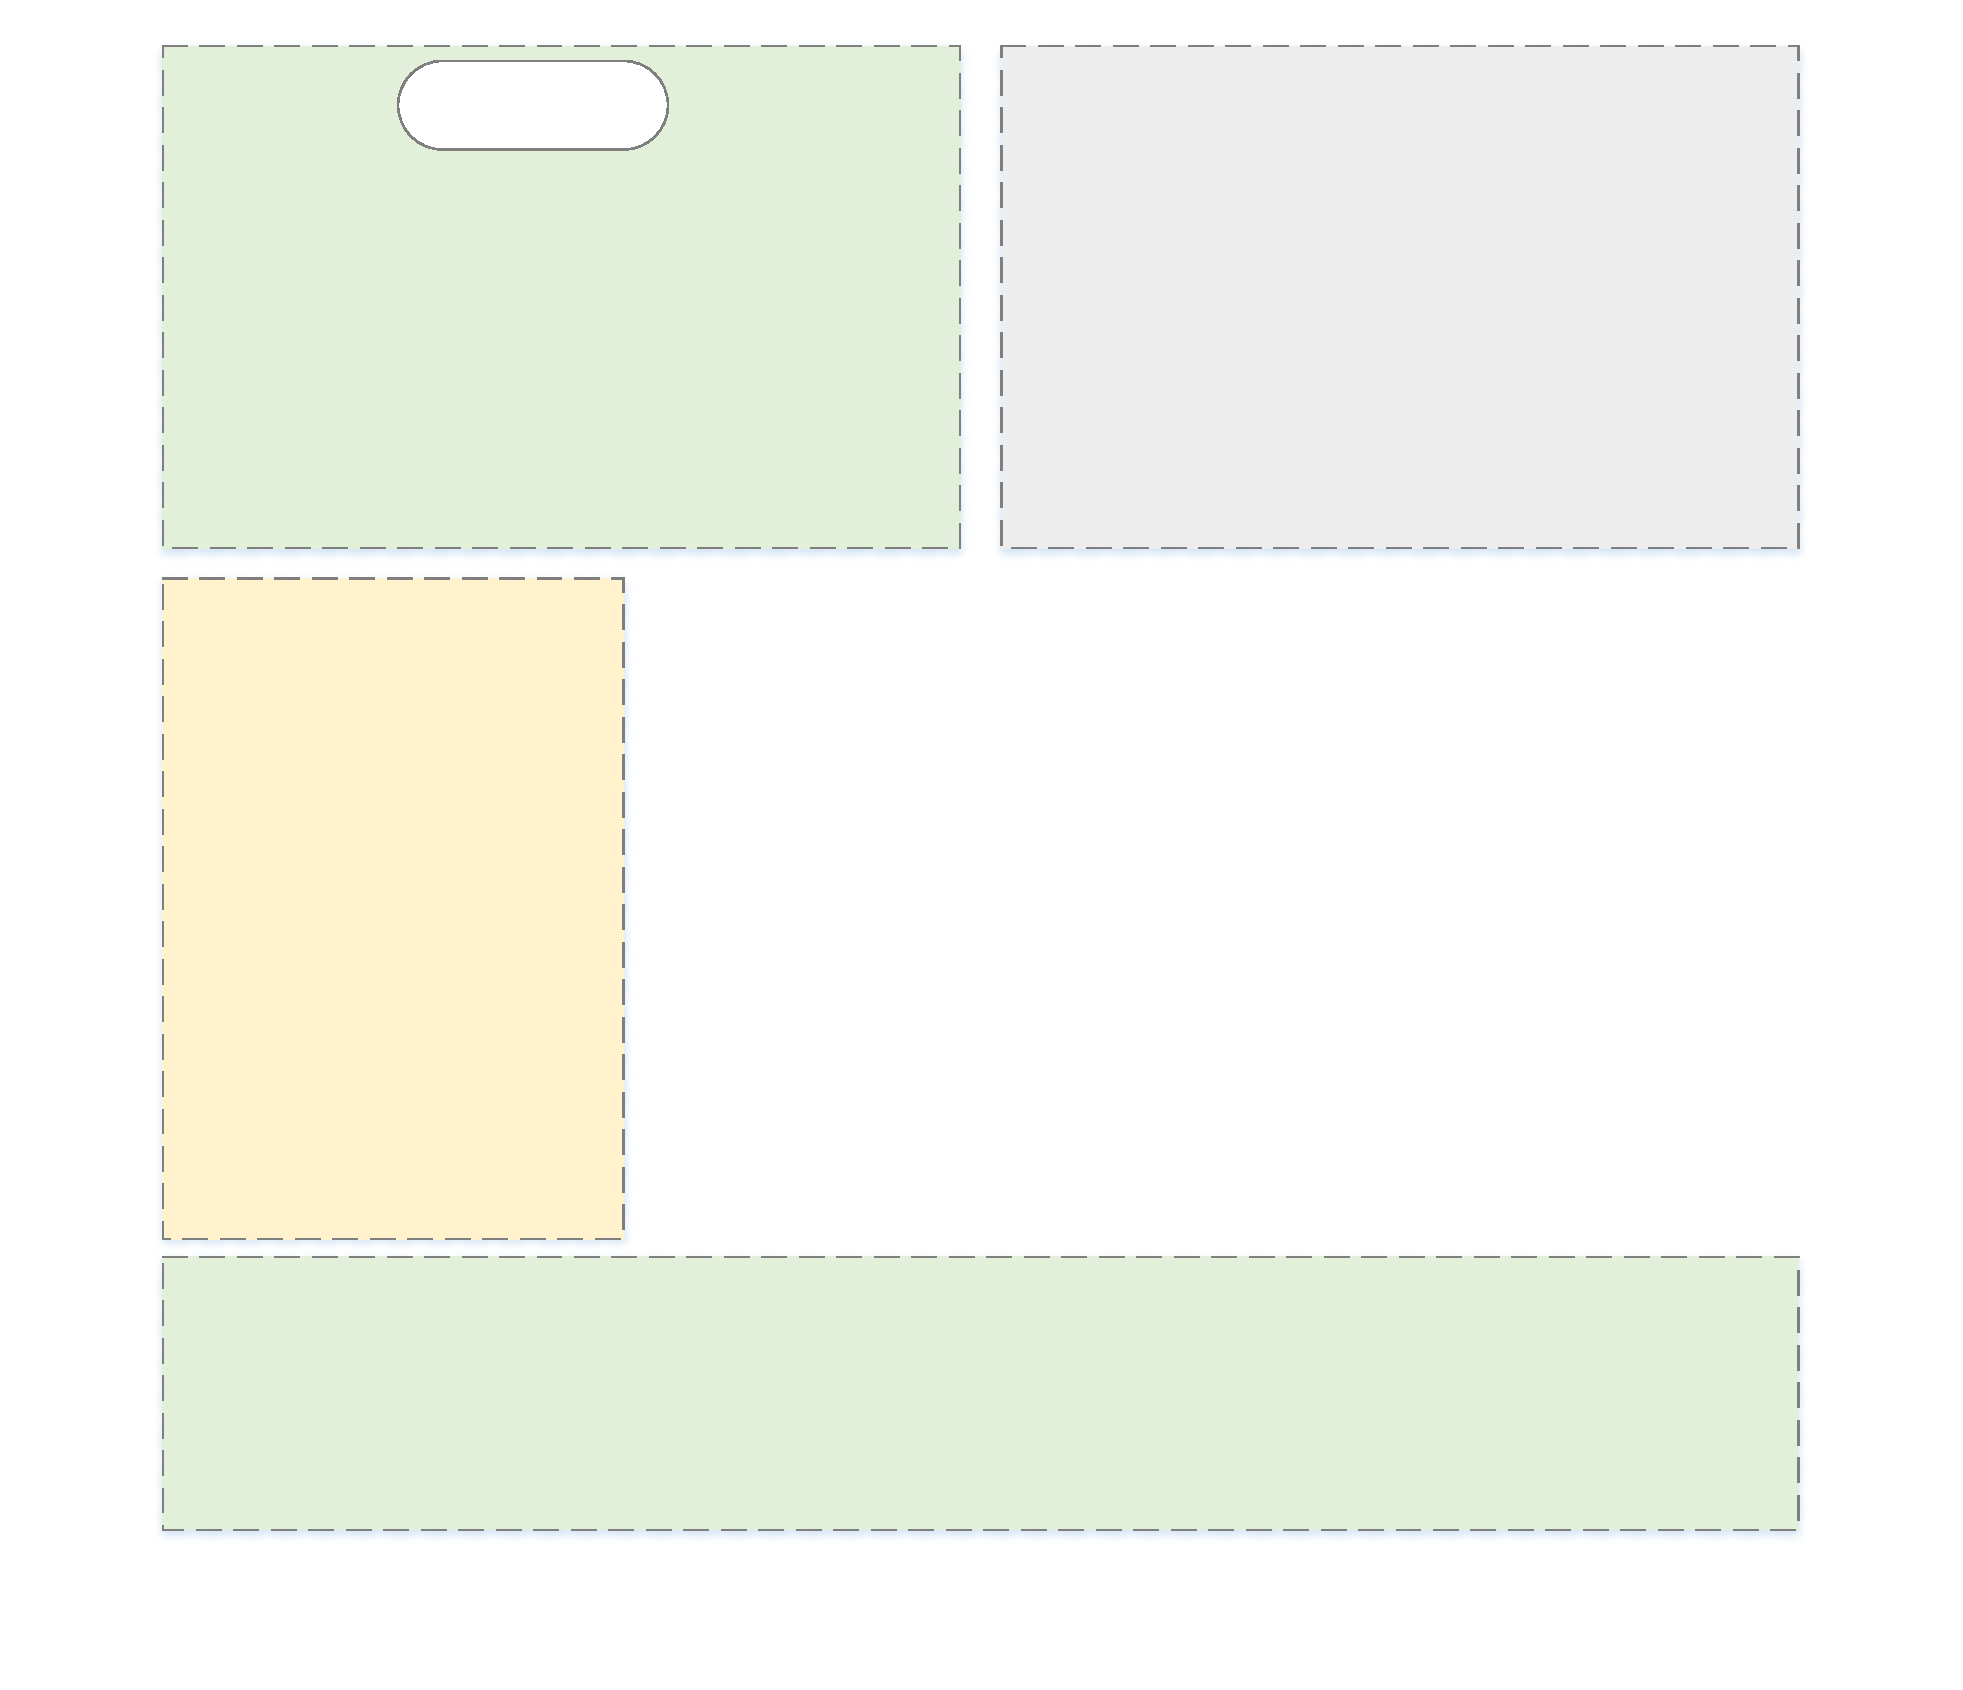
\includegraphics[width=\textwidth]{images/pakcet_life_2020}
	%\caption{Figure: Inspection Stage}
	%\label{fig:system:pakcet_life_2020}
%\end{figure}

\begin{figure}
    \centering
    \includesvg{1.6\columnwidth}{../images/pakcet_life_2020}
    %\caption{Figure}
\end{figure}

\pdfbookmark[1]{Packet Handling Sequence}{Packet Handling Sequence}
\section*{\hypertarget{link:Packet Handling Sequence}{Packet Handling Sequence}}
\label{sec:appendix_e:sequence}

\pdfbookmark[2]{Ingress stage}{Ingress stage}
\subsection*{\hypertarget{link:Ingress stage}{Ingress stage}}
\label{sec:appendix_e:sequence:ingress}

The ingress stage receives packets from the network interface, parses those packets, and then determines whether a given packet is subject to further inspection. If the packet is subject to further inspection, the system continues with a session lookup and the packet enters the session stage. Otherwise, the system forwards the packet to the egress stage.

\pdfbookmark[3]{Layer 2 Decode}{Layer 2 Decode}
\subsubsection*{\hypertarget{link:Layer 2 Decode}{Layer 2 Decode}}
\label{sec:appendix_e:sequence:ingress:decode}

Packet parsing starts with the Ethernet (Layer-2) header of the packet received from the wire. VLAN, MPLS, MAC\_IN\_MAC headers are parsed here. The ingress port, 802.1q tag, and destination MAC address are used as keys to lookup the ingress logical interface. 

\pdfbookmark[3]{Tunnel Decapsulation}{Tunnel Decapsulation}
\subsubsection*{\hypertarget{link:Tunnel Decapsulation}{Tunnel Decapsulation}}
\label{sec:appendix_e:sequence:ingress:decapsulation}

If the packet has PPPOE, IPIP, GRE, PPTP, L2TP, Teredo, GTP encapsulations, they are decoded at this stage.

\pdfbookmark[3]{IP Defragmentation}{IP Defragmentation}
\subsubsection*{\hypertarget{link:IP Defragmentation}{IP Defragmentation}}
\label{sec:appendix_e:sequence:ingress:defragmentation}

After the IP header is parsed (Layer-3), the TSG parses IP fragments, reassembles using the defragmentation process, and then feeds the packet back to the parser starting with the IP header.  At this stage, a fragment may be discarded due to tear-drop attack (overlapping fragments), fragmentation errors, or if the TSG hits system limits on buffered fragments (hits the max packet threshold).

\pdfbookmark[2]{Session Setup}{Session Setup}
\subsection*{\hypertarget{link:Session Setup}{Session Setup}}
\label{sec:appendix_e:sequence:setup}

If the packet is subject to firewall inspection, it performs a flow lookup on the packet. In TSG ’s implementation, the firewall identifies the flow using a 5-tuple key:


• Source and destination IP addresses: IP addresses from the IP packet. 


• Source and destination ports: Port numbers from TCP/UDP protocol headers. For non-TCP/UDP, different protocol fields are used (e.g., for ICMP the ICMP identifier and sequence numbers are used).


• Protocol: The IP protocol number from the IP header is used to derive the flow key. 


The firewall stores active flows in the flow lookup table. When a packet is determined to be eligible for firewall inspection, the firewall extracts the 5-tuple flow key from the packet and then performs a flow lookup to match the packet with an existing flow. Each flow has a client and server component. For TCP, the client is the sender of the TCP SYN packet of the session from firewall’s perspective. For UDP, the client is the sender with smaller Port number. The server is the receiver of this first packet. 


If the packet belongs to on new session, firewall performs a session setup.


The firewall uses the IP address of the packet to query mapping tables.


• Subscriber-IP mapping table: The corresponding user information is fetched.


• ASN-IP mapping table: The autonomous system number is fetched.


• Geo-IP mapping table: The geographical location is fetched.


There is a chance that above information is not available at this point. In that case, policies with these conditions cannot be enforced.

\pdfbookmark[2]{Session Maintenance}{Session Maintenance}
\subsection*{\hypertarget{link:Session Maintenance}{Session Maintenance}}
\label{sec:appendix_e:sequence:maintenance}

A packet that matches an existing session will enter the session maintenance stages. This stage starts with Layer 2 to Layer 4 firewall processing:


• If the session is in close wait state, then the firewall discards the packet by forwarding to egress stage. 


• If the session is active, refresh session timeout.


• If the packet is a TCP FIN/RST, the session TCP half closed timer is started if this is the first FIN packet received (half closed session) or the TCP Time Wait timer is started if this is the second FIN packet or RST packet. The session is closed as soon as either of these timers expire. 


If an application uses TCP as the transport, the firewall processes it by the TCP reassembly module before it sends the data stream into the security-processing module. The TCP reassembly module will also perform window check, buffer out-of-order data while skipping TCP retransmission. The firewall drops the packets if there is a reassembly error or if it receives too many out-of-order fragments, resulting in the reassembly buffers filling up.


A packet matching an existing session is subject to further processing if packet has TCP/UDP data (payload). If the firewall does not detect the session application, it performs application identification. If the identification is non-conclusive, the content inspection module runs known protocol decoder checks and heuristics to help identify the application. The application identification result could change throughout the life of the session. Once a traffic attribute is parsed, it’s subject to security policy enforcement.

\pdfbookmark[2]{Firewall Process}{Firewall Process}
\subsection*{\hypertarget{link:Firewall Process}{Firewall Process}}
\label{sec:appendix_e:sequence:firewall}

\pdfbookmark[3]{Layer 7 Decode}{Layer 7 Decode}
\subsubsection*{\hypertarget{link:Layer 7 Decode}{Layer 7 Decode}}
\label{sec:appendix_e:sequence:firewall:decode}

The firewall decodes Layer 7 protocols such as HTTP, SSL/TLS and DNS, to get traffic attributes.

\pdfbookmark[3]{Application Identification}{Application Identification}
\subsubsection*{\hypertarget{link:Application Identification}{Application Identification}}
\label{sec:appendix_e:sequence:firewall:identification}

The firewall identifies application with built-in and customized signature. The firewall uses protocol decoding in the content inspection stage to determine if an application changes from one application to another. After the firewall identifies the session application, security policy will be enforced as configured. 

\pdfbookmark[3]{Content Decode}{Content Decode}
\subsubsection*{\hypertarget{link:Content Decode}{Content Decode}}
\label{sec:appendix_e:sequence:firewall:contentdecode}

The firewall decodes the flow and parses attributes and content, then scan them for keywords, e.g., email attachments that are text-based. If it results in keywords detection, then the corresponding security policy action is taken. Application identification is still on at this stage, as the more traffic attributes are parsed, application identification result may be changed. 

\pdfbookmark[3]{Security Policy Lookup}{Security Policy Lookup}
\subsubsection*{\hypertarget{link:Security Policy Lookup}{Security Policy Lookup}}
\label{sec:appendix_e:sequence:firewall:lookup}

The firewall uses application ANY, IP, port, Geographic and Subscriber ID to perform the lookup and check for a rule match. In case of a rule match, if the policy action is set to ‘deny’, the firewall drops the packet. 


If security policy action is set to intercept and the application is SSL or HTTP, the firewall sends session packets to Proxy to perform decryption.


After more packet transferred, identified application as well as FQDN, URL and applicable protocol fields in the session are used as key to find rule match. If the session matches a security rule, and the rule has logging enabled, the firewall generates a security event log at the session end.

\pdfbookmark[2]{Proxy Process}{Proxy Process}
\subsection*{\hypertarget{link:Proxy Process}{Proxy Process}}
\label{sec:appendix_e:sequence:proxy}

\pdfbookmark[3]{Duplicate Packet Processing}{Duplicate Packet Processing}
\subsubsection*{\hypertarget{link:Duplicate Packet Processing}{Duplicate Packet Processing}}
\label{sec:appendix_e:sequence:proxy:duplicate}

Packet usually travels a route one time only, otherwise it’s a waste of bandwidth. But network of real world is complicated: tunnels, policy ACLs and human mistakes all induce packet travels a link more than one time.


This will cause problems on Proxy function. When Proxy terminates server-side SSL connections, as a client, it sends packet to server with original 4-tuple, and that packet goes through TSG again. Since this packet has the same 4-tuple and sequence number as the client-side, TSG will drop it as a client-side retransmission packet, which causes server-side timeout.


The proxy fixes this problem by following two mechanisms:


• Duplicate packet identification: For TSG sent packets, TSG adds its 4-tuple, IPID, acknowledge number, sequence number and timestamp (if applicable) to the Bloom filter. For received packet, TSG will query the Bloom filter with the aforementioned protocol fields. If a packet is considered duplicate, it will be bypassed, if not, it will be delivered to TCP stack.


• Duplicate flow detection: Since not all traffic flows have duplicate packets, do duplicate identification on each packet is a waste of CPU and memory, moreover, it induces performance overhead. Hence, only the TCP flows with duplicate SYN or SYN/ACK packet will conduct duplicate packet identification. 

\pdfbookmark[3]{TCP Stack}{TCP Stack}
\subsubsection*{\hypertarget{link:TCP Stack}{TCP Stack}}
\label{sec:appendix_e:sequence:proxy:TCP}

Opening a TCP connection involves a three-way handshake involving packets: the client contacts the server, the server acknowledges the client, and the client acknowledges the server. The proxy’s TCP stack attempts to connect server-side immediately after receiving the client's initial connection request, but waits to return the server acknowledgement until determining whether or not the server-side connection succeeds. This provides greater transparency, as the client receives either an RST or no response, which mirrors what is sent from a server when connections fail.

\pdfbookmark[3]{Build SSL Session}{Build SSL Session}
\subsubsection*{\hypertarget{link:Build SSL Session}{Build SSL Session}}
\label{sec:appendix_e:sequence:proxy:build}

The proxy first builds server-side SSL session, if the server certificate verification is failed, the proxy will sign certificate with untrusted root. That’s because the proxy wants the untrust certificate to warn users that they are trying to access potentially unsafe sites.

\pdfbookmark[3]{Proxy Policy Lookup}{Proxy Policy Lookup}
\subsubsection*{\hypertarget{link:Proxy Policy Lookup}{Proxy Policy Lookup}}
\label{sec:appendix_e:sequence:proxy:lookup}

After decode Layer 7 protocols, traffic attributes like HTTP URL, headers are subject to proxy policy lookup, then according action is taken.

\pdfbookmark[3]{Re-encryption}{Re-encryption}
\subsubsection*{\hypertarget{link:Re-encryption}{Re-encryption}}
\label{sec:appendix_e:sequence:proxy:re-encryption}

The content is compressed and encrypted, and send to egress stage

\pdfbookmark[2]{Egress Stage}{Egress Stage}
\subsection*{\hypertarget{link:Egress Stage}{Egress Stage}}
\label{sec:appendix_e:sequence:egress}

The system identifies encapsulation information for the packet, including MAC addresses, VLAN ID and tunnel headers. And find the egress interface.
Finally, the packet is transmitted out of the physical egress interface.
         % INCLUDE: Appendix_E
\cleardoublepage
% !TEX root = ../TSG_Administrator's_Guide_Latest_EN.tex
%
%\pdfbookmark[0]{Appendix F Best Practices}{Appendix F Best Practices}
\chapter*{\hypertarget{link:Appendix F Best Practices}{Appendix F Best Practices}}
\addcontentsline{toc}{chapter}{Appendix F Best Practices}
\label{sec:appendix_f}

%\pdfbookmark[1]{Security Policy}{Appendix Security Policy}
\section*{\hypertarget{link:Appendix Security Policy}{Security Policy}}
\addcontentsline{toc}{section}{Security Policy}
\label{sec:appendix_f:policy}

To improve your overall security posture, use the guidelines in this section to plan, deploy, and maintain your internet gateway best practices security policy. Apply security best practices to gain visibility into traffic, prevent threats, and protect your network, users, and data. 


\textbf{The first use case} is to deny SSL traffic based on SNI. For example, users are forbidden to visit Netflix pages.

\begin{description}[leftmargin=0pt,itemindent=0em]
    \item[] 
    \begin{enumerate}
        \item Without any policies, visit Netflix website and you can view it normally.
        \item	Create a Deny Security Policy:
        \begin{enumerate}
            \item 	After logging into the system, create a Security Policy.
            \item	Policy names can be defined according to user habits.
            \item	Action select Deny.
            \item	Specify client IP as matching criteria for the source field. 
            \item	Application select SSL.
            \item	Specify the Netflix page you wish to deny as matching criteria for SNI field.  
            \item	Select Drop as Sub Action.
            \item	Enable the policy and submit.
        \end{enumerate}
        \item	Visit Netflix again and pages cannot be accessed.
    \end{enumerate}	
\end{description}

\textbf{The second use case} is monitor mails based on specified keywords. This Security Policy will generate a Security Event Log when matched.

\begin{description}[leftmargin=0pt,itemindent=0em]
    \item[] 
    \begin{enumerate}
        \item	Create a Monitor Security Policy:
        \begin{enumerate}
            \item	After logging into the system, create a Security Monitor Policy.
            \item	Policy names can be defined according to user habits.
            \item	Action select Monitor.
            \item	Specify client IP as matching criteria for the source field. 
            \item	Application select MAIL.
            \item	Specify the keywords you wish to monitor as matching criteria for Content field.  
            \item	Enable the policy and submit.
        \end{enumerate}        
        \item	When the policy is matched, you can view Logs > Security Events and see the mail content.
    \end{enumerate}	
\end{description}

%\pdfbookmark[1]{Proxy Policy}{Appendix Proxy Policy}
\section*{\hypertarget{link:Appendix Proxy Policy}{Proxy Policy}}
\addcontentsline{toc}{section}{Proxy Policy}
\label{sec:appendix_f:proxy}

The growth in SSL/TLS encrypted traffic traversing the internet is on an explosive upturn. We are going to take five use case to demonstrate proxy policy best practices. 


\textbf{The first use case} is to specifically deny HTTPS traffic based on the URL. For example, users are forbidden to visit specific pages of YouTube, but other pages of YouTube website are not affected.

\begin{description}[leftmargin=0pt,itemindent=0em]
    \item[] 
    \begin{enumerate}
        \item	Without any policies, visit YouTube website and you can view it normally.
        \item	Create a Deny Policy:
        \begin{enumerate}
            \item	After logging into the system, create a policy.
            \item	Policy names can be defined according to user habits.
            \item	Action select Deny.
            \item	Specify client IP as matching criteria for the source field. Specify the YouTube page you wish to deny as matching criteria for URL field.  
            \item	You can select the Response Content of the blocking page as an optional parameter.
            \item	Enable the policy and submit.
        \end{enumerate}	
        \item	Visit YouTube again. The specified pages cannot be accessed and other pages can be accessed normally.
    \end{enumerate}	
\end{description}

\textbf{The second use case} is URL redirect, such as redirect the traffic accessing Google to Bing.

\begin{description}[leftmargin=0pt,itemindent=0em]
    \item[] 
    \begin{enumerate}
        \item	Without any policies, you can visit Google normally and search normally.
        \item	Create a redirect policy. The above has demonstrated how to create a policy, to save time, simply enable the policy that which was created before. Then click Edit to view the content of the policy.
        \begin{enumerate}
            \item	Action is Redirect.
            \item	Filter is Google URL.
            \item	Redirect URL is Bing URL.
            \item	The policy is Enabled and click OK.
        \end{enumerate}
        \item	Visit Google again and the page is redirected to Bing.
    \end{enumerate}	
\end{description}

\textbf{The third use case} is content Replace. For example, search china in Google. Create a content Replace policy to make the search results only come from www.news.cn.

\begin{description}[leftmargin=0pt,itemindent=0em]
    \item[] 
    \begin{enumerate}
        \item	Without any policies, search china in Google and you’ll see the search results come from different websites, wikis, etc.
        \item	Create a Replace policy:
        \begin{enumerate}
            \item	Action select Replace.
            \item	Add Google URL as Filter.
            \item	Specify Action Parameters:
            \begin{enumerate}
                \item	Replace “q=china” in HTTP Request URI with “q=china+site%3Awww.news.cn”.
                \item	Replace “china site:www.news.cn” in HTTP Response Body with “china”.
            \end{enumerate}	
            \item	Enable the policy and submit. 
        \end{enumerate}	
        \item	Visit Google again, search china and you’ll see the search results only come from www.news.cn.
    \end{enumerate}	
\end{description}

\textbf{The fourth use case} is hijack file. For example, download the WhatsApp installation package and replace it with other files, such as the WhatsApp installation package with trojan virus. Now replace it with test.exe is used Instead.

\begin{description}[leftmargin=0pt,itemindent=0em]
    \item[] 
    \begin{enumerate}
        \item	Without any policies, it is normal to download the WhatsApp installation package.
        \item	Create a Hijack policy:
        \begin{enumerate}
            \item	Action select Hijack.
            \item	Select WhatsApp download URL as Filter.
            \item	Select test.exe as Hijack File for Action Parameters.
            \item	Enable the policy and submit.
        \end{enumerate}
        \item	Download WhatsApp again and find that the actual download file is test.exe. If you do not want to be found easily, you can change the hijack file into the same name as the original.
    \end{enumerate}	
\end{description}

\textbf{The fifth use case} is script injection. For example, visit Facebook, insert the script into Facebook page, and the script will be executed on the client side. Here we use a JS script of pop-up window will show up to demonstrate. 

\begin{description}[leftmargin=0pt,itemindent=0em]
    \item[] 
    \begin{enumerate}
        \item	Without any policies, visit Netflix website and it displays normally without any pop-up window.
        \item	Create an Insert policy:
        \begin{enumerate}
            \item	Action select Insert.
            \item	Select Netflix URL as Filter.
            \item	Select the JS script of pop-up window as Insert Script for Action Parameters.
            \item	Enable the policy and submit.
        \end{enumerate}	
        \item	Visit the Netflix website again, and the pop-up window appears.
    \end{enumerate}	
\end{description}

\notemark\textit{The Watch feature only support policy and object. You can add them to your watch list. Select the checkbox for objects and policies in the list and Click \textbf{Watch} at the bottom to add to Watch List. And then you can click the star icon in the bottom right and select Object/Policy tab to view the Watch List. You can search objects and policies by ID and Name in the list. For policy, you can check policy in the list and enable or disable it. You can also export and clear the list.}

%\pdfbookmark[1]{Custom Application}{Custom Application}
\section*{\hypertarget{link:Custom Application}{Custom Application}}
\addcontentsline{toc}{section}{Custom Application}
\label{sec:appendix_f:application}

A policy object consists of one item or a set of collective items that groups discrete identities such as IP addresses, URLs, applications, or accounts. The relationship between each item is “or”. However, for keyword, within each item, there can be “and” expression and the item can have up to 4 substrings. You can reference the object in policy as conditions. The relationship between each condition within policy is “and”. There can be eight conditions at most for every policy.


Application is a little special as a kind of object in TSG. Applications increase the value of our TSG firewalls by making it easier and faster to determine the exact identity of applications traversing the network, enabling teams to set and enforce the right policies. Applications can reduce complexity and minimize human error. 


The following introduced predefined application attributes:


TCP/UDP/IP Attributes

\begin{longtable}{p{0.35\textwidth}|p{0.11\textwidth}|p{0.08\textwidth}|p{0.14\textwidth}}   
    \rowcolor{black}\multicolumn{1}{l!\vlinewhite}{\textcolor{white}{Attribute Name}} & \multicolumn{1}{l!\vlinewhite}{\textcolor{white}{Layer}} & \multicolumn{1}{l!\vlinewhite}{\textcolor{white}{Stage}} & \textcolor{white}{Value Type} \\\hline  
    IP Address


    ip.src &	Packet &	0 &	ip \\ \hline
    ip.dst &	Packet &	0 &	ip \\ \hline
    tcp.payload.c2s\_first\_data &	Session &	1 &	string \\ \hline
    tcp.payload.s2c\_first\_data &	Session &	2 &	string \\ \hline
    tcp.analysis.create\_with\_syn &	Session &	1 &	Bool \\ \hline
    ip.payload &	Packet &	0 &	string \\ \hline
    tcp.payload &	Packet &	0 &	string \\ \hline
    tcp.srcport &	Packet &	0 &	Numeric \\ \hline
    tcp.dstport &	Packet &	0 &	Numeric \\ \hline
    tcp.syn.fingerprint &	Session &	1 &	string \\ \hline
    tcp.sack.fingerprint &	Session &	1 &	string \\ \hline
    udp.payload.c2s\_first\_data &	Session &	0 &	string \\ \hline
    udp.payload.s2c\_first\_data &	Session &	1 &	string \\ \hline
    udp.srcport &	Packet &	0 &	Numeric \\ \hline
    udp.dstport &	Packet &	0 &	Numeric \\ \hline    
\end{longtable}

SSL Attributes

\begin{longtable}{p{0.61\textwidth}|p{0.11\textwidth}|p{0.08\textwidth}|p{0.14\textwidth}}   
    \rowcolor{black}\multicolumn{1}{l!\vlinewhite}{\textcolor{white}{Attribute Name}} & \multicolumn{1}{l!\vlinewhite}{\textcolor{white}{Layer}} & \multicolumn{1}{l!\vlinewhite}{\textcolor{white}{Stage}} & \textcolor{white}{Value Type} \\\hline   
    ssl.handshake.extensions\_server\_name &	Session &	1 &	string \\ \hline
    ssl.handshake.cert.fingerprint &	Session &	2 &	string \\ \hline
    ssl.handshake.cert.serial\_number &	Session &	2 &	string \\ \hline
    ssl.handshake.certificate.issuer\_common\_name &	Session &	2 &	string \\ \hline
    ssl.handshake.certificate.issuer\_organization\_name &	Session &	2 &	string \\ \hline
    ssl.handshake.certificate.issuer\_country\_name &	Session &	2 &	string \\ \hline
    ssl.handshake.certificate.subject\_common\_name &	Session &	2 &	string \\ \hline
    ssl.handshake.certificate.subject\_organization\_name &	Session &	2 &	string \\ \hline
    ssl.handshake.certificate.subject\_country\_name &	Session &	2 &	string \\ \hline
    ssl.handshake.certificate.not\_valid\_before &	Session &	2 &	string \\ \hline
    ssl.handshake.certificate.not\_valid\_after &	Session &	2 &	string \\ \hline
    ssl.handshake.certificate.algorithm\_id &	Session &	2 &	string \\ \hline
    ssl.analysis.use\_session\_resumption &	Session &	3 &	Numeric \\ \hline
    ssl.analysis.use\_selfsigned\_certificate &	Session &	3 &	Numeric \\ \hline
    ssl.analysis.incomplete\_certificate\_chain &	Session &	3 &	Numeric \\ \hline    
\end{longtable}

\notemark\textit{Client Hello is in Stage 1, and Server Hello is in Stage 2. SSL Attributes are all in Session Layer.}

HTTP Attributes

\begin{longtable}{p{0.35\textwidth}|p{0.11\textwidth}|p{0.08\textwidth}|p{0.14\textwidth}}   
    \rowcolor{black}\multicolumn{1}{l!\vlinewhite}{\textcolor{white}{Attribute Name}} & \multicolumn{1}{l!\vlinewhite}{\textcolor{white}{Layer}} & \multicolumn{1}{l!\vlinewhite}{\textcolor{white}{Stage}} & \textcolor{white}{Value Type} \\\hline  
    http.host &	Session &	1 &	string \\ \hline
    http.uri &	Session &	1 &	string \\ \hline
    http.user\_agent &	Session &	1 &	string \\ \hline
    http.content\_type &	Session &	1 &	string \\ \hline
    http.content\_encoding &	Session &	1 &	string \\ \hline
    http.referer &	Session &	1 &	string \\ \hline
    http.cookie &	Session &	1 &	string \\ \hline
    http.set\_cookie &	Session &	3 &	string \\ \hline   
\end{longtable}

\notemark\textit{HTTP Request Header, Request Body, Response Header, Response Body are in Stage 1, Stage 2, Stage 3, Stage 4 in sequence. HTTP attributes are all in Session Layer.}


Other Attributes

\begin{longtable}{p{0.35\textwidth}|p{0.11\textwidth}|p{0.08\textwidth}|p{0.14\textwidth}}   
    \rowcolor{black}\multicolumn{1}{l!\vlinewhite}{\textcolor{white}{Attribute Name}} & \multicolumn{1}{l!\vlinewhite}{\textcolor{white}{Layer}} & \multicolumn{1}{l!\vlinewhite}{\textcolor{white}{Stage}} & \textcolor{white}{Value Type} \\\hline  
    quic.sni &	Session &	1 &	string \\ \hline
    dns.qry.name &	Session &	1 &	string \\ \hline
    general.session.analysis.app\_id &	Session &	2 &	numeric \\ \hline
    general.c2s\_session\_size &	Session &	2 &	string \\ \hline
    general.s2c\_session\_size &	Session &	2 &	string \\ \hline     
\end{longtable}

%\pdfbookmark[1]{Make Your Own Reports}{Make Your Own Reports}
\section*{\hypertarget{link:Make Your Own Reports}{Make Your Own Reports}}
\addcontentsline{toc}{section}{Make Your Own Reports}
\label{sec:appendix_f:report}

The following guides you to set a report with one type of chart. Of course, you can create a report with all types of charts by TSG function \textbf{Reports}.

%\pdfbookmark[2]{The 1st: Bar}{The 1st: Bar}
\subsection*{\hypertarget{link:The 1st: Bar}{The 1$^{st}$: Bar}}
\addcontentsline{toc}{subsection}{The 1$^{st}$: Bar}
\label{sec:appendix_f:report:bar}

Create a Bar Report. For example, make a report about the top 10 server IP that our security policy matched last week and the sum of bytes sent and bytes received from that server IP.

\begin{description}
    \item[STEP 1.]	Create a Dataset. Dataset specify what data to extract from logs.
    \begin{enumerate}
        \item Select \textbf{Reports} > \textbf{Datasets} menu, and click \textbf{Create}.
        \item Enter a \textbf{Name}, security event bytes by server IP dataset.
        \item Select a \textbf{Log Type}: Security Event.
        \item Select the \textbf{Group by}. This will serve as the X-Axis Data Binding options for Chart Libraries. The report mainly displays Server IP, so select Server IP.
        \item Specify the \textbf{Data Bindings}, add field, aggregate, and label, which serve as Y-Axis Data Binding options of your Chart Libraries. Field consists of the Group by field you just added. You can add one or multiple fields. Field select bytes Sent and bytes Received. Aggregate select sum. Label set to bytes-Sum. 
        \item Specify \textbf{Filter} and \textbf{Having}. For Filter, select Action as Field; select “=” as Operator; select Monitor and Intercept as Value. That is to say, only security policies with monitor and intercept actions will be counted. For Having, select Log ID as Field; select count as Aggregate; select “>=” as Operator; select 10 as value. This means only security policies that match more than 10 times (including 10) will be counted. Your selections will automatically generate a SQL.
        \item Click \textbf{OK}.  
    \end{enumerate}
    \item[STEP 2.]	Create Chart Library. Chart set the display form of the data.
    \begin{enumerate}
        \item	Enter a \textbf{Name} and \textbf{Description}. Complete name, security event bytes by server IP Chart Library. Leave description set to empty. 
        \item	Select the \textbf{Dataset} you just created.
        \item	Select \textbf{Chart Type}: Bar. 
        \item	Set the \textbf{Data Bindings} for X-Axis and Y-Axis. Set Show Top to 10. Set Label, which will be displayed in your report.
        \item	Click \textbf{OK}.
    \end{enumerate}
    \item[STEP 3.]	Create a Report.
    \begin{enumerate}
        \item	Enter a \textbf{Name}, security event bytes by server IP report.
        \item	Select a \textbf{Time Period}. Here select last 1 week, which is from yyyy-mm-dd-7 hh:mi:ss to yyyy-mm-dd hh:mi:ss.
        \item	Select the \textbf{Chart Library} you just created. 
        \item	Click \textbf{OK}.
    \end{enumerate}
\end{description}

%\pdfbookmark[2]{The 2nd: Line}{The 2nd: Line}
\subsection*{\hypertarget{link:The 2nd: Line}{The 2$^{nd}$: Line}}
\addcontentsline{toc}{subsection}{The 2$^{nd}$: Line}
\label{sec:appendix_f:report:line}

Create a Line Report. For example, make a report about the security event sessions count previous day.

\begin{description}
    \item[STEP 1.]	Create a Dataset. Dataset specify what data to extract from logs.
    \begin{enumerate}
        \item Select \textbf{Reports} > \textbf{Datasets} menu, and click \textbf{Create}.
        \item Enter a \textbf{Name}, security event sessions by time dataset.
        \item Select a \textbf{Log Type}: Security Event.
        \item Select the \textbf{Group by}. For Line Chart, you must select Receive Time. This will serve as the X-Axis Data Binding options for Chart Libraries.
        \item Specify the \textbf{Data Bindings}, add field, aggregate, and label, which serve as Lines Data Binding options of your Chart Libraries. Field consists of the Group by field you just added. You can add one or multiple fields. Field select Log ID. Aggregate select count. Label set to count. 
        \item Click \textbf{OK}.
    \end{enumerate}
    \item[STEP 2.]	Create Chart Library. Chart set the display form of the data.
    \begin{enumerate}
        \item Enter a \textbf{Name} and \textbf{Description}. Complete name, security event sessions by time Chart Library. Leave description set to empty.
        \item Select the \textbf{Dataset} you just created.
        \item Select \textbf{Chart Type}: Line. 
        \item Set the \textbf{Data Bindings} for X-Axis and Lines. For Lines, select count as Data Binding; select Counter(K/M/G) as Format; select Line Up as Type; input count as Legend. 
        \item Click \textbf{OK}.
    \end{enumerate}
    \item[STEP 3.]	Create a Report.
    \begin{enumerate}
        \item Enter a \textbf{Name}, security event sessions by time report.
        \item Select a \textbf{Time Period}. Here select previous 1 day, which means from yyyy-mm-dd-1 00:00:00 to yyyy-mm-dd-1 23:00:00 if the Time Granularity is 1 hour.
        \item Select the \textbf{Chart Library} you just created. Enter number and select time unit for \textbf{Time Granularity}. Here set it to 1 hour.
        \item Click \textbf{OK}.
    \end{enumerate}
\end{description}

%\pdfbookmark[2]{The 3rd: Drilldown}{The 3rd: Drilldown}
\subsection*{\hypertarget{link:The 3rd: Drilldown}{The 3$^{rd}$: Drilldown}}
\addcontentsline{toc}{subsection}{The 3$^{rd}$: Drilldown}
\label{sec:appendix_f:report:drilldown}

Create a Drilldown Report. For example, make a report about the session count for top 100 Http.Domain, Drilldown on Subscriber ID and show Drilldown top 5 that our security policy matched last week.

\begin{description}
    \item[STEP 1.]	Create a Dataset. Dataset specify what data to extract from logs.
    \begin{enumerate}
        \item Select \textbf{Reports} > \textbf{Datasets} menu, and click Create.
        \item Enter a \textbf{Name}, security event session top domain and subscriber IDs drilldown dataset.
        \item Select a \textbf{Log Type}: Security Event.
        \item Select the \textbf{Group by}. The report mainly displays Http.Domain and Subscriber ID, so add Http.Domain and Subscriber ID.
        \item Specify the \textbf{Data Bindings}, add field, aggregate, and label, which serve as Columns options of your Chart Libraries. Field consists of the Group by field you just defined and you can add other fields. Here add Log ID; select count as Aggregate and set Label to sessions.
        \item Specify \textbf{Filter} and \textbf{Having}. For Filter, select Address Type as Field; select “=” as Operator; select IPv4 as Value. That is to say, only security policies with IPv4 address type will be counted. For Having, select Log ID as Field; select count as Aggregate; select “>=” as Operator; select 10 as value. This means only security policies that match more than 10 times (including 10) will be counted. Your selections will automatically generate a SQL.
        \item Click \textbf{OK}.
    \end{enumerate}
    \item[STEP 2.]	Create Chart Library. Chart set the display form of the data.
    \begin{enumerate}
        \item Enter a \textbf{Name} and \textbf{Description}. Complete name, security event session top domain and subscriber IDs drilldown chart. Leave description set to empty. 
        \item Select the \textbf{Dataset} you just created.
        \item Select \textbf{Chart Type}: Table. 
        \item For \textbf{Data Bindings}, select Drilldown as Table Type. Drilldown tables have three columns and you must select one as drilldown column. Complete Title, Width, Data Binding, Format and Legend for each column. And enable Drilldown Columns for Subscriber ID. Select order by sessions descending. Show Top 100 Http.Domains. Drilldown Top 5 on Subscriber ID.
        \item Click \textbf{OK}.
    \end{enumerate}
    \item[STEP 3.]	Create a Report. 
    \begin{enumerate}
        \item Enter a \textbf{Name}, security event session top domain and subscriber IDs drilldown report.
        \item Select a \textbf{Time Period}. Here select last 1 week, which is from yyyy-mm-dd-7 hh:mi:ss to yyyy-mm-dd hh:mi:ss.
        \item \textbf{Enable Notification}, select Email as Output Profile. 
        

              Email: Enter recipient's e-mail.
        \item Select the \textbf{Chart Library} you just created.
        \item Click \textbf{OK}.
    \end{enumerate}
\end{description}

%\pdfbookmark[2]{The 4th: Double-lines}{The 4th: Double-lines}
\subsection*{\hypertarget{link:The 4th: Double-lines}{The 4$^{th}$: Double-lines}}
\addcontentsline{toc}{subsection}{The 4$^{th}$: Double-lines}
\label{sec:appendix_f:report:double-lines}

Create a top N Line Report. For example, make a report about the session count group by Http.Domain (top 5) every day that our security policy matched in the last month.

\begin{description}
    \item[STEP 1.]	Create a Dataset. Dataset specify what data to extract from logs.
    \begin{enumerate}
        \item Select \textbf{Reports} > \textbf{Datasets} menu, and click \textbf{Create}.
        \item Enter a \textbf{Name}, security event counter by domain dataset.
        \item Select a \textbf{Log Type}: Security Event.
        \item Select the \textbf{Group by}. For Line Chart, you must select Receive Time. This will serve as the X-Axis Data Binding options for Chart Libraries. The report mainly displays Http.Domain, so add Http.Domain. This will be added to your Group by option in your Chart Libraries.
        \item Specify the \textbf{Data Bindings}, add field, aggregate, and label. Field consists of the Group by field you just added. You can add other fields. Field select Log ID. Aggregate select count. Label set to counter.
        \item Click \textbf{OK}.
    \end{enumerate}
    \item[STEP 2.]	Create Chart Library. Chart set the display form of the data.
    \begin{enumerate}
        \item Enter a \textbf{Name} and \textbf{Description}. Complete name, security event counter by domain chart. Leave description set to empty.
        \item Select the \textbf{Dataset} you just created.
        \item Select \textbf{Chart Type}: Line. 
        \item Set the \textbf{Data Bindings} for X-Axis and Lines. For Lines, select counter as Data Binding; select Default as Format; select Line Up as Type; input counter as Legend. Check Group by and select Http.Domain. Check Order by and select counter. Check Descending. Max line is 5.
        \item Click \textbf{OK}.
    \end{enumerate}
    \item[STEP 3.]	Create a Report. 
    \begin{enumerate}
        \item Enter a \textbf{Name}, security event counter by domain report.
        \item Select a \textbf{Time Period}. Here select last 1 month, which is from yyyy-(mm-1)-dd hh:mi:ss to yyyy-mm-dd hh:mi:ss.
        \item Select the \textbf{Chart Library} you just created. Enter number and select time unit for \textbf{Time Granularity}. Here set it to 1 day.
        \item Add \textbf{Filter}. Select Http.Domain as Field; select notEmpty as Operator. This means, empty domain name will not be counted.
        \item Click \textbf{OK}.
    \end{enumerate}
\end{description}

%\pdfbookmark[2]{The 5th: Area}{The 5th: Area}
\subsection*{\hypertarget{link:The 5th: Area}{The 5$^{th}$: Area}}
\addcontentsline{toc}{subsection}{The 5$^{th}$: Area}
\label{sec:appendix_f:report:area}

Create an Area Report. For example, make a report about the sum of bytes Sent and bytes Received and the sum of Packets Sent and Packets Received every day that our security policy matched in last month.

\begin{description}
    \item[STEP 1.]	Create a Dataset. Dataset specify what data to extract from logs.
    \begin{enumerate}
        \item Select \textbf{Reports} > \textbf{Datasets} menu, and click \textbf{Create}.
        \item Enter a \textbf{Name}, security event bytes and packets dataset.
        \item Select a \textbf{Log Type}: Security Event.
        \item Select the \textbf{Group by}. For Area Chart, you must select Receive Time. This will serve as the X-Axis (TimeLine) Data Binding options for Chart Libraries. You can add other Fields, which will be added to your Group by options in your Chart Libraries.
        \item Specify the \textbf{Data Bindings}, add field, aggregate, and label. Field consists of the Group by field you just added. You can add other fields. Field select bytes Sent and bytes Received; aggregate select sum; label set to bytes. Field select Packets Sent and Packets Received; aggregate select sum; label set to Packets.
        \item Click \textbf{OK}.
    \end{enumerate}
    \item[STEP 2.]	Create Chart Library. Chart set the display form of the data.
    \begin{enumerate}
        \item Enter a \textbf{Name} and \textbf{Description}. Complete name, security event bytes and packets chart. Leave description set to empty.
        \item Select the \textbf{Dataset} you just created.
        \item Select \textbf{Chart Type}: Area. 
        \item Set the \textbf{Data Bindings} for X-Axis and Lines. For Lines, select bytes as Data Binding; select Bandwidth (Kbps/Mbps/Gbps) as Format; select Line Up as Type; input bytes as Legend. Select Packets as Data Binding; select Bandwidth (Kpps/Mpps/Gpps) as Format; select Line Down as Type; input Packets as Legend.
        \item Click \textbf{OK}.
    \end{enumerate}
    \item[STEP 3.]	Create a Report. 
    \begin{enumerate}
        \item Enter a \textbf{Name}, security event bytes and packets report. 
        \item Select a \textbf{Time Period}. Here select last 1 month, which is from yyyy-(mm-1)-dd hh:mi:ss to yyyy-mm-dd hh:mi:ss.
        \item Select the \textbf{Chart Library} you just created. Enter number and select time unit for \textbf{Time Granularity}. Here set it to 1 day.
        \item Click \textbf{OK}.
    \end{enumerate}
\end{description}

%\pdfbookmark[2]{The 6th: Network Behavior Analysis for Specific User }{The 6th: Network Behavior Analysis for Specific User }
\subsection*{\hypertarget{link:The 6th: Network Behavior Analysis for Specific User }{The 6$^{th}$: Network Behavior Analysis for Specific User }}
\addcontentsline{toc}{subsection}{The 6$^{th}$: Network Behavior Analysis for Specific User}
\label{sec:appendix_f:report:6th}

Create a report to analyze network behavior of specific user, such as specific IP address or Subscriber ID. For example, create a report for Internal IP 192.168.50.2. It will include 9 charts and tables, that display traffic trend, top access domain and top access URLs based on sessions. 

\begin{description}
    \item[STEP 1.]	Create 3 Datasets. Select \textbf{Reports} > \textbf{Datasets} menu, and click \textbf{Create}. Select the same Log Type for the 3 datasets: Session Records.
    \begin{enumerate}
        \item Create a Dataset with \textbf{Name} Traffic-Metrics-Trend.
        \begin{enumerate}
            \item	Select Receive Time as \textbf{Group by}. 
            \item	Specify the \textbf{Data Bindings}, add field, aggregate, and label. You can add multiple items for data bindings once and reference the same dataset when creating multiple charts. Now add 7 items. 
            \begin{enumerate}
                \item	Field select Bytes Sent and Bytes Received; aggregate select sum; Label set to bytes. 
                \item	Field select Bytes Sent; aggregate select sum; Label set to Bytes Sent. 
                \item	Field select Bytes Received; aggregate select sum; Label set to Bytes Received. 
                \item	Field select sessions; aggregate select sum; Label set to New sessions. 
                \item	Field select Packets Sent and Packets Received; aggregate select sum; Label set to Packets.
                \item	Field select Packets Sent; aggregate select sum; Label set to Packets Sent.
                \item	Field select Packets Received; aggregate select sum; Label set to Packets Received.
            \end{enumerate}
            \item	Click \textbf{OK}.
        \end{enumerate}
        \item Create a Dataset with \textbf{Name} Traffic-Top-Access-Domain.
        \begin{enumerate}
            \item	Select Http.Domain as \textbf{Group by}.
            \item	Specify the \textbf{Data Bindings}, add field, aggregate, and label. Field select Sessions; aggregate select sum; label set to Sessions.
            \item	Specify \textbf{Filter}. Select Http.Domain as Field; select notEmpty as Operator. This configuration will exclude empty domains. 
            \item	Click \textbf{OK}.
        \end{enumerate}
        \item Create a Dataset with \textbf{Name} Traffic-Top-Access-URL.
        \begin{enumerate}
            \item	Select Http.URL as \textbf{Group by}.
            \item	Specify the \textbf{Data Bindings}, add field, aggregate, and label. Field select Sessions; aggregate select sum; label set to Sessions.
            \item	Specify \textbf{Filter}. Select Http.URL as Field; select notEmpty as Operator. This configuration will exclude empty URLs. 
            \item	Click \textbf{OK}.
        \end{enumerate}
    \end{enumerate}
    \item[STEP 2.]	 Create 9 Chart Libraries. Chart set the display form of the data. Select \textbf{Reports} > \textbf{Chart Library} menu, and click Create.
    \begin{enumerate}
        \item 	Create a Chart Library with \textbf{Name} Traffic Bandwidth Trend.
        \begin{enumerate}
            \item 	Select \textbf{Dataset} Traffic-Metrics-Trend.
            \item 	Select \textbf{Chart Type}: Area.
            \item 	Set the \textbf{Data Bindings} for X-Axis and Lines. Select Receive Time defined in Group By from dataset as X-Axis. Select Time as Format. You can add multiple Data Binding for Lines.
            \begin{enumerate}
                \item	Select Bytes as Data Binding; select Bandwidth (Kbps/Mbps/Gbps) as Format; select Line Up as Type; input total as Legend. 
                \item	Select Bytes Sent as Data Binding; select Bandwidth (Kbps/Mbps/Gbps) as Format; select Line Up as Type; input out as Legend.
                \item	 Select Bytes Received as Data Binding; select Bandwidth (Kbps/Mbps/Gbps) as Format; select Line Up as Type; input in as Legend.
            \end{enumerate}
            \item 	 Click \textbf{OK}.
        \end{enumerate}
        \item 	Create a Chart Library with \textbf{Name} Traffic Packet Trend.
        \begin{enumerate}
            \item 	Select \textbf{Dataset} Traffic-Metrics-Trend.
            \item 	Select \textbf{Chart Type}: Area.
            \item 	Set the \textbf{Data Bindings} for X-Axis and Lines. Select Receive Time defined in Group By from dataset as X-Axis. Select Time as Format. You can add multiple Data Binding for Lines.
            \begin{enumerate}
                \item	Select Packets as Data Binding; select Bandwidth(Kpps/Mpps/Gpps) as Format; select Line Up as Type; input total as Legend. 
                \item	Select Packets Sent as Data Binding; select Bandwidth (Kpps/Mpps/Gpps) as Format; select Line Up as Type; input out as Legend.
                \item	Select Packets Received as Data Binding; select Bandwidth (Kpps/Mpps/Gpps) as Format; select Line Up as Type; input in as Legend.
            \end{enumerate}
            \item 	Click \textbf{OK}.
        \end{enumerate}
        \item 	Create a Chart Library with \textbf{Name} Traffic New Sessions Trend.
        \begin{enumerate}
            \item 	Select \textbf{Dataset} Traffic-Metrics-Trend.
            \item 	Select \textbf{Chart Type}: Line.
            \item 	Set the \textbf{Data Bindings} for X-Axis and Lines. Select Receive Time defined in Group By from dataset as X-Axis. Select Time as Format. Select New Sessions as Data Binding; select Counter(K/M/G) as Format; select Line Up as Type; input New Sessions as Legend.
            \item 	Click \textbf{OK}.
        \end{enumerate}
        \item 	Create a Chart Library with \textbf{Name} Traffic Top 30 Access Domains Detail.
        \begin{enumerate}
            \item 	Select \textbf{Dataset} Traffic-Top-Access-Domain.
            \item 	Select \textbf{Chart Type}: Table.
            \item 	For \textbf{Data Bindings}, select Regular as Table Type. Click to add Column. Complete Title, Width, Data Binding, Format and Legend for each column. Fill in Domain as Title; select Domain as Data Binding; input Domain as Legend. Fill in Sessions as Title; select Sessions as Data Binding; select Counter(K/M/G) as Format; input Sessions as Legend. Select order by Sessions descending. Show Top 30.
            \item 	Click \textbf{OK}.
        \end{enumerate}
        \item 	Create a Chart Library with \textbf{Name} Traffic Top 30 Access Domains Distribution.
        \begin{enumerate}
            \item 	Select \textbf{Dataset} Traffic-Top-Access-Domain.
            \item 	Select \textbf{Chart Type}: Bar.
            \item 	Set the \textbf{Data Bindings} for X-Axis and Y-Axis. For X-Axis, select Domain as Data Binding; set Domain as Label; set Show Top to 30. For Y-Axis, select Sessions as Data Binding; select Counter(K/M/G) as Format; set Label to Sessions.
            \item 	Click \textbf{OK}.
        \end{enumerate}
        \item 	Create a Chart Library with \textbf{Name} Traffic Top 10 Access Domains Percent.
        \begin{enumerate}
            \item 	Select \textbf{Dataset} Traffic-Top-Access-Domain.
            \item 	Select \textbf{Chart Type}: Pie.
            \item 	Set the \textbf{Data Bindings} for Category and Series. For Category, select Domain as Data Binding; set Domain as Label; set Show Top to 10. For Series, select Sessions as Data Binding; select Counter(K/M/G) as Format; set Label to Sessions. Check Bundle rest into ‘Others’.
            \item 	Click \textbf{OK}.
        \end{enumerate}
        \item 	Create a Chart Library with \textbf{Name} Traffic Top 30 Access URLS Detail.
        \begin{enumerate}
            \item 	Select \textbf{Dataset} Traffic-Top-Access-URL.
            \item 	Select \textbf{Chart Type}: Table.
            \item 	For \textbf{Data Bindings}, select Regular as Table Type. Click to add Column. Complete Title, Width, Data Binding, Format and Legend for each column. Fill in URL as Title; select URL as Data Binding; input URL as Legend. Fill in Sessions as Title; select Sessions as Data Binding; select Counter(K/M/G) as Format; input Sessions as Legend. Select order by Sessions descending. Show Top 30.
            \item 	Click \textbf{OK}.
        \end{enumerate}
        \item 	Create a Chart Library with \textbf{Name} Traffic Top 30 Access URLS Distribution.
        \begin{enumerate}
            \item 	Select \textbf{Dataset} Traffic-Top-Access-URL.
            \item 	Select \textbf{Chart Type}: Bar.
            \item 	Set the \textbf{Data Bindings} for X-Axis and Y-Axis. For X-Axis, select URL as Data Binding; set URL as Label; set Show Top to 30. For Y-Axis, select Sessions as Data Binding; select Counter(K/M/G) as Format; set Label to Sessions.
            \item 	Click \textbf{OK}.
        \end{enumerate}
        \item 	Create a Chart Library with \textbf{Name} Traffic Top 10 Access URLS Percent.
        \begin{enumerate}
            \item 	Select \textbf{Dataset} Traffic-Top-Access-URL.
            \item 	Select \textbf{Chart Type}: Pie.
            \item 	Set the \textbf{Data Bindings} for Category and Series. For Category, select URL as Data Binding; set URL as Label; set Show Top to 10. For Series, select Sessions as Data Binding; select Counter(K/M/G) as Format; set Label to Sessions. Check Bundle rest into ‘Others’.
            \item 	Click \textbf{OK}.
        \end{enumerate}
    \end{enumerate}
    \item[STEP 3.]	Create a Report. 
    \begin{enumerate}
        \item 	Enter a \textbf{Name}, Traffic Report with Internal IP 192.168.50.2. 
        \item 	Select a \textbf{Time Period}. Select last 1 day.
        \item 	Select the \textbf{Chart Library} you just created. Click Add Chart to add multiple charts.
        \begin{enumerate}
            \item	Select Traffic Bandwidth Trend. Set 5 minutes for \textbf{Time Granularity}.
            \item	Select Traffic Packets Trend. Set 5 minutes for \textbf{Time Granularity}.
            \item	Select Traffic New Sessions Trend. Set 5 minutes for \textbf{Time Granularity}.
            \item	Select Traffic Top 30 Access Domains Detail.
            \item	Select Traffic Top 30 Access Domains Distribution.
            \item	Select Traffic Top 10 Access Domains Percent.
            \item	Select Traffic Top 30 Access URLS Detail.
            \item	Select Traffic Top 30 Access URLS Distribution.
            \item	Select Traffic Top 10 Access URLS Percent.
        \end{enumerate}
        \item 	Specify \textbf{Filter}. Select Internal IP as Field; select “=” as Operator; set Value to 192.168.50.2.  
        \item 	Click \textbf{OK}.
    \end{enumerate}
\end{description}

%\pdfbookmark[2]{The 7th: Website Access Analysis for Specific Domain}{The 7th: Website Access Analysis for Specific Domain}
\subsection*{\hypertarget{link:The 7th: Website Access Analysis for Specific Domain}{The 7$^{th}$: Website Access Analysis for Specific Domain}}
\addcontentsline{toc}{subsection}{The 7$^{th}$: Website Access Analysis for Specific Domain}
\label{sec:appendix_f:report:7th}

Create a report to analyze website access of specific domain, such as google.com. For example, create a custom report to analyze security events which hit google.com. It will include 5 charts and tables, that display traffic trend based on bandwidth and client IP number, security event action hit sessions trend and and top Server IP based on sessions.

\begin{description}
    \item[STEP 1.]	Create 3 Datasets. Select \textbf{Reports} > \textbf{Datasets} menu, and click \textbf{Create}. Select the same \textbf{Log Type} for the 3 datasets: Security Event.
    \begin{enumerate}
        \item Create a Dataset with \textbf{Name} Security-Intercept-Event-Metrics-Trend.
        \begin{enumerate}
            \item 	Select Receive Time as \textbf{Group by}. 
            \item 	Specify the \textbf{Data Bindings}, add field, aggregate, and label. You can add multiple items for data bindings. Now add 2 items. 
            \begin{enumerate}
                \item	Field select Bytes Sent and Bytes Received; aggregate select sum; Label set to Bytes. 
                \item	Field select Client IP; aggregate select count distinct; Label set to Unique Client IP. 
            \end{enumerate}
            \item 	Specify \textbf{Filter}. Select Action as Field; select “=” as Operator; set Value to Intercept. This configuration will only include Security Events with intercept action. 
            \item 	Click \textbf{OK}.
        \end{enumerate}
        \item Create a Dataset with \textbf{Name} Security-Event-Action-Hit-Sessions-Trend.
        \begin{enumerate}
            \item 	Select Receive Time and Action as \textbf{Group by}. 
            \item 	Specify the \textbf{Data Bindings}, add field, aggregate, and label. Field select Log ID; Label set to Sessions. 
            \item 	Click \textbf{OK}.
        \end{enumerate}
        \item Create a Dataset with \textbf{Name} Security-Event-Top-Server-IP.
        \begin{enumerate}
            \item 	Select Server IP as \textbf{Group by}. 
            \item 	Specify the \textbf{Data Bindings}, add field, aggregate, and label. Field select Log ID; Label set to Sessions. 
            \item 	Click \textbf{OK}.
        \end{enumerate}
    \end{enumerate}
    \item[STEP 2.]	Create 5 Chart Libraries. Chart set the display form of the data. Select \textbf{Reports} > \textbf{Chart Library} menu, and click Create.
    \begin{enumerate}
        \item Create a Chart Library with \textbf{Name} Security Intercept Event Metrics Trend.
        \begin{enumerate}
            \item 	Select \textbf{Dataset} Security-Intercept-Event-Metrics-Trend.
            \item 	Select \textbf{Chart Type}: Line.
            \item 	Set the \textbf{Data Bindings} for X-Axis and Lines. Select Receive Time defined in Group By from dataset as X-Axis. Select Time as Format. For Lines, select Unique Client IP as Data Binding; select Counter(K/M/G) as Format; select Line Up as Type; input Unique Client IP as Legend. Select Bytes as Data Binding; select Bandwidth(Kbps/Mbps/Gbps) as Format; select Line Down as Type; input bps as Legend.
            \item 	Click \textbf{OK}.
        \end{enumerate}
        \item Create a Chart Library with \textbf{Name} Security Event Action Hit Sessions Trend.
        \begin{enumerate}
            \item 	Select \textbf{Dataset} Security-Event-Action-Hit-Sessions-Trend.
            \item 	Select \textbf{Chart Type}: Line.
            \item 	Set the \textbf{Data Bindings} for X-Axis and Lines. Select Receive Time defined in Group By from dataset as X-Axis. Select Time as Format. For Lines, select sessions as Data Binding; select Counter(K/M/G) as Format; select Line Up as Type; input sessions as Legend. Check Group By and select Action. Check Order By, select sessions and check Descending. Show Top 10.
            \item 	Click \textbf{OK}.
        \end{enumerate}
        \item Create a Chart Library with \textbf{Name} Security Event Top 30 Server IP Detail.
        \begin{enumerate}
            \item 	Select \textbf{Dataset} Security-Event-Top-Server-IP.
            \item 	Select \textbf{Chart Type}: Table.
            \item 	For \textbf{Data Bindings}, select Regular as Table Type. Click to add Column. Complete Title, Width, Data Binding, Format and Legend for each column. Fill in Server IP as Title; select Server IP as Data Binding; input Server IP as Legend. Fill in Sessions as Title; select Sessions as Data Binding; select Counter(K/M/G) as Format; input Sessions as Legend. Select order by Sessions descending. Show Top 30.
            \item 	Click \textbf{OK}.
        \end{enumerate}
        \item Create a Chart Library with \textbf{Name} Security Event Top 30 Server IP Distribution.
        \begin{enumerate}
            \item 	Select \textbf{Dataset} Security-Event-Top-Server-IP.
            \item 	Select \textbf{Chart Type}: Bar.
            \item 	Set the \textbf{Data Bindings} for X-Axis and Y-Axis. For X-Axis, select Server IP as Data Binding; set Server IP as Label; set Show Top to 30. For Y-Axis, select Sessions as Data Binding; select Counter(K/M/G) as Format; set Label to Sessions.
            \item 	Click \textbf{OK}.
        \end{enumerate}
        \item Create a Chart Library with \textbf{Name} Security Event Top 10 Server IP Percent.
        \begin{enumerate}
            \item 	Select \textbf{Dataset} Security-Event-Top-Server-IP.
            \item 	Select \textbf{Chart Type}: Pie.
            \item 	Set the \textbf{Data Bindings} for Category and Series. For Category, select Server IP as Data Binding; set Server IP as Label; set Show Top to 10. For Series, select Sessions as Data Binding; select Counter(K/M/G) as Format; set Label to Sessions. Check Bundle rest into ‘Others’.
            \item 	Click \textbf{OK}.
        \end{enumerate}
    \end{enumerate}
    \item[STEP 3.]	Create a Report. 
    \begin{enumerate}
        \item Enter a \textbf{Name}, Security Event Report with Domain google.com. 
        \item Select a \textbf{Time Period}. Select last 1 day.
        \item Select the \textbf{Chart Library} you just created. Click Add Chart to add multiple charts.
        \begin{enumerate}
            \item 	Select Security Intercept Event Metrics Trend. Set 5 minutes for \textbf{Time Granularity}.
            \item 	Select Security Event Action Hit Sessions Trend. Set 5 minutes for \textbf{Time Granularity}.
            \item 	Select Security Event Top 30 Server IP Detail. Set 5 minutes for \textbf{Time Granularity}.
            \item 	Select Security Event Top 30 Server IP Distribution.
            \item 	Select Security Event Top 10 Server IP Percent.
        \end{enumerate}
        \item Specify \textbf{Filter}. Select Http.Domain as Field; select “=” as Operator; set Value to google.com.  
        \item Click \textbf{OK}.
    \end{enumerate}
\end{description}

%\pdfbookmark[2]{The 8th: Endpoints Access Analysis for Specific City}{The 8th: Endpoints Access Analysis for Specific City}
\subsection*{\hypertarget{link:The 8th: Endpoints Access Analysis for Specific City}{The 8$^{th}$: Endpoints Access Analysis for Specific City}}
\addcontentsline{toc}{subsection}{The 8$^{th}$: Endpoints Access Analysis for Specific City}
\label{sec:appendix_f:report:8th}

Customize a report to analyze endpoints access of specific Data Center. For example, create a report to analyze session records about endpoints information in specific Data Center. It will include 2 charts and tables, that display number of Unique External IP, Internal IP and Subscriber ID trend based on bandwidth and show Unique client IP number and Unique Subscriber ID number of Top 100 domains.

\begin{description}
    \item[STEP 1.]	Create 2 Datasets. Select \textbf{Reports} > \textbf{Datasets} menu, and click \textbf{Create}. Select the same \textbf{Log Type} for the 2 datasets: Session Records.
    \begin{enumerate}
        \item Create a Dataset with \textbf{Name} Traffic-Endpoints-Metrics-Trend.
        \begin{enumerate}
            \item	Select Receive Time as \textbf{Group by}. 
            \item	Specify the \textbf{Data Bindings}, add field, aggregate, and label. You can add multiple items for data bindings. Now add 5 items. 
            \begin{enumerate}
                \item	Field select Bytes Sent and Bytes Received; aggregate select sum; Label set to Bytes. 
                \item	Field select Sessions; aggregate select sum; Label set to Sessions.
                \item	Field select Internal IP; aggregate select count distinct; Label set to Unique Internal IP. 
                \item	Field select External IP; aggregate select count distinct; Label set to Unique External IP.
                \item	Field select Subscriber ID; aggregate select count distinct; Label set to Unique Subscriber ID.
            \end{enumerate}
            \item	Click \textbf{OK}.
        \end{enumerate}
        \item Create a Dataset with \textbf{Name} Traffic-Top-Domain-with-Unique-Client-IP-and-Subscriber-ID.
        \begin{enumerate}
            \item	Select Http.Domain as \textbf{Group by}. 
            \item	Specify the \textbf{Data Bindings}, add field, aggregate, and label. You can add multiple items for data bindings. Now add 2 items. 
            \begin{enumerate}
                \item	Field select Client IP; aggregate select count distinct; Label set to Unique Client IP. 
                \item	Field select Subscriber ID; aggregate select count distinct; Label set to Unique Subscriber ID.
            \end{enumerate}
            \item	Specify \textbf{Filter}. Select Http.Domain as Field; select notEmpty as Operator. This configuration will exclude Session Records with empty domain. 
            \item	Click \textbf{OK}.
        \end{enumerate}
    \end{enumerate}
    \item[STEP 2.]	Create 2 Chart Libraries. Chart set the display form of the data. Select \textbf{Reports} > \textbf{Chart Library} menu, and click Create.
    \begin{enumerate}
        \item Create a Chart Library with \textbf{Name} Traffic Endpoints Metrics Trend.
        \begin{enumerate}
            \item 	Select \textbf{Dataset} Traffic-Endpoints-Metrics-Trend.
            \item 	Select \textbf{Chart Type}: Line.
            \item 	Set the \textbf{Data Bindings} for X-Axis and Lines. Select Receive Time defined in Group By from dataset as X-Axis. Select Time as Format. For Lines, select Unique External IP as Data Binding; select Counter(K/M/G) as Format; select Line Up as Type; input Unique External IP as Legend; select Unique Internal IP as Data Binding; select Counter(K/M/G) as Format; select Line Up as Type; input Unique Internal IP as Legend; select Unique Subscriber ID as Data Binding; select Counter(K/M/G) as Format; select Line Up as Type; input Unique Subscriber ID as Legend. Select Bytes as Data Binding; select Bandwidth(Kbps/Mbps/Gbps) as Format; select Line Down as Type; input bps as Legend.
            \item 	Click \textbf{OK}.
        \end{enumerate}
        \item Create a Chart Library with \textbf{Name} Traffic Top 100 Domains with Unique Client IP and Subscriber ID.
        \begin{enumerate}
            \item 	Select \textbf{Dataset} Traffic-Top-Domain-with-Unique-Client-IP-and-Subscriber-ID.
            \item 	Select \textbf{Chart Type}: Table.
            \item 	For \textbf{Data Bindings}, select Regular as Table Type. Click to add Column. Complete Title, Width, Data Binding, Format and Legend for each column. Fill in Domain as Title; select Http.Domain as Data Binding; input Http.Domain as Legend. Fill in Unique Client IP as Title; select Unique Client IP as Data Binding; select Counter(K/M/G) as Format; input Unique Client IP as Legend. Fill in Unique Subscriber ID as Title; select Unique Subscriber ID as Data Binding; select Counter(K/M/G) as Format; input Unique Subscriber ID as Legend. Select order by Unique Client IP descending. Show Top 100.
            \item 	Click \textbf{OK}.
        \end{enumerate}
    \end{enumerate}
    \item[STEP 3.]	Create a Report. 
    \begin{enumerate}
        \item Enter a \textbf{Name}, Traffic Report with Data Center DC1 and DC2. 
        \item Select a \textbf{Time Period}. Select last 1 day.
        \item Select the \textbf{Chart Library} you just created. Click Add Chart to add multiple charts.
        \begin{enumerate}
            \item	Select Traffic Endpoints Metrics Trend. Set 5 minutes for \textbf{Time Granularity}.
            \item	Select Traffic Top 100 Domains with Unique Client IP and Subscriber ID.
        \end{enumerate}
        \item Specify \textbf{Filter}. Select Data Center as Field; select “=” as Operator; set Value to DC1 and DC2. 
        \item Click \textbf{OK}.
    \end{enumerate}
\end{description}

%\pdfbookmark[2]{The 9th: Endpoints Details Analysis for Intercept Action }{The 9th: Endpoints Details Analysis for Intercept Action }
\subsection*{\hypertarget{link:The 9th: Endpoints Details Analysis for Intercept Action }{The 9$^{th}$: Endpoints Details Analysis for Intercept Action }}
\addcontentsline{toc}{subsection}{The 9$^{th}$: Endpoints Details Analysis for Intercept Action}
\label{sec:appendix_f:report:9th}

Customize a report to analyze endpoints details of intercept action. For example, create a report to analyze Security Events about multiple dimensional endpoints information. It will include 8 charts and tables, that display endpoints statistics details, including Top Client IP, Server IP, Internal IP, External IP (by Sessions with Bandwidth), Top Domain Distribution (by Sessions with Bandwidth), Top Domain Drilldown Internal IP (by Sessions), Top Domain Drilldown Server IP (by Bandwidth), Top Subscriber ID Drilldown Domain (by Sessions). With the help of this example, you can have a better understanding of the meaning of Drilldown table and bar charts and how to create them.

\begin{description}
    \item[STEP 1.]	Create 8 Datasets. Select \textbf{Reports} > \textbf{Datasets} menu, and click \textbf{Create}. Select the same \textbf{Log Type} for the 2 datasets: Security Event.
    \begin{enumerate}
        \item Create a Dataset with \textbf{Name} Security-Event-Top-Internal-IP-by-Sessions-with-Bandwidth.
        \begin{enumerate}
            \item	Select Internal IP as \textbf{Group by}. 
            \item	Specify the \textbf{Data Bindings}, add field, aggregate, and label. You can add multiple items for data bindings. Now add 4 items. 
            \begin{enumerate}
                \item	Field select Bytes Sent and Bytes Received; aggregate select sum; Label set to Bytes. 
                \item	Field select Bytes Sent; aggregate select sum; Label set to Bytes Sent. 
                \item	Field select Bytes Received; aggregate select sum; Label set to Bytes Received. 
                \item	Field select Log ID; Label set to Sessions.
            \end{enumerate}
            \item	Click \textbf{OK}.
        \end{enumerate}
        \item Create a Dataset with \textbf{Name} Security-Event-Top-External-IP-by-Sessions-with-Bandwidth.
        \begin{enumerate}
            \item	Select External IP as \textbf{Group by}. 
            \item	Specify the \textbf{Data Bindings}, add field, aggregate, and label. You can add multiple items for data bindings. Now add 4 items. 
            \begin{enumerate}
                \item	Field select Bytes Sent and Bytes Received; aggregate select sum; Label set to Bytes. 
                \item	Field select Bytes Sent; aggregate select sum; Label set to Bytes Sent. 
                \item	Field select Bytes Received; aggregate select sum; Label set to Bytes Received. 
                \item	Field select Log ID; Label set to Sessions.
            \end{enumerate}
            \item	Click \textbf{OK}.
        \end{enumerate}
        \item Create a Dataset with \textbf{Name} Security-Event-Top-Client-IP-by-Sessions-with-Bandwidth.
        \begin{enumerate}
            \item	Select Client IP as \textbf{Group by}. 
            \item	Specify the \textbf{Data Bindings}, add field, aggregate, and label. You can add multiple items for data bindings. Now add 4 items. 
            \begin{enumerate}
                \item	Field select Bytes Sent and Bytes Received; aggregate select sum; Label set to Bytes. 
                \item	Field select Bytes Sent; aggregate select sum; Label set to Bytes Sent. 
                \item	Field select Bytes Received; aggregate select sum; Label set to Bytes Received. 
                \item	Field select Log ID; Label set to Sessions.
            \end{enumerate}
            \item	Click \textbf{OK}.
        \end{enumerate}
        \item Create a Dataset with \textbf{Name} Security-Event-Top-Server-IP-by-Sessions-with-Bandwidth.
        \begin{enumerate}
            \item	Select Server IP as \textbf{Group by}. 
            \item	Specify the \textbf{Data Bindings}, add field, aggregate, and label. You can add multiple items for data bindings. Now add 4 items. 
            \begin{enumerate}
                \item	Field select Bytes Sent and Bytes Received; aggregate select sum; Label set to Bytes. 
                \item	Field select Bytes Sent; aggregate select sum; Label set to Bytes Sent. 
                \item	Field select Bytes Received; aggregate select sum; Label set to Bytes Received. 
                \item	Field select Log ID; Label set to Sessions.
            \end{enumerate}
            \item	Click \textbf{OK}.
        \end{enumerate}
        \item Create a Dataset with \textbf{Name} Security-Event-Top-Domain-by-Sessions.
        \begin{enumerate}
            \item	Select Http.Domain as \textbf{Group by}. 
            \item	Specify the \textbf{Data Bindings}, add field, aggregate, and label. You can add multiple items for data bindings. Field select Log ID; Label set to Sessions.
            \item	Specify \textbf{Filter}. Select Http.Domain as Field; select notEmpty as Operator. This configuration will exclude Security Events with empty Domain.
            \item	Click \textbf{OK}.
        \end{enumerate}
        \item Create a Dataset with \textbf{Name} Security-Event-Top-Domain-by-Internal-IP-and-Sessions.
        \begin{enumerate}
            \item	Select Http.Domain and Internal IP as \textbf{Group by}. 
            \item	Specify the \textbf{Data Bindings}, add field, aggregate, and label. You can add multiple items for data bindings. Field select Log ID; Label set to Sessions.
            \item	Specify \textbf{Filter}. Select Http.Domain as Field; select notEmpty as Operator. This configuration will exclude Security Events with empty Domain.
            \item	Click \textbf{OK}.
        \end{enumerate}
        \item Create a Dataset with \textbf{Name} Security-Event-Top-Domain-by-Server-IP-and-Bandwidth.
        \begin{enumerate}
            \item	Select Http.Domain and Server IP as \textbf{Group by}. 
            \item	Specify the \textbf{Data Bindings}, add field, aggregate, and label. You can add multiple items for data bindings. Field select Bytes Sent and Bytes Received; aggregate select sum; Label set to Bytes.
            \item	Specify \textbf{Filter}. Select Http.Domain as Field; select notEmpty as Operator. This configuration will exclude Security Events with empty Domain.
            \item	Click \textbf{OK}.
        \end{enumerate}
        \item Create a Dataset with \textbf{Name} Security-Event-Top-Subscriber-ID-by-Website-Domains-and-Sessions.
        \begin{enumerate}
            \item	Select Http.Domain and Subscriber ID as \textbf{Group by}. 
            \item	Specify the \textbf{Data Bindings}, add field, aggregate, and label. You can add multiple items for data bindings. Field select Log ID; Label set to Sessions.
            \item	Specify \textbf{Filter}. You can add multiple items. Select Http.Domain as Field; select notEmpty as Operator. Click add and select Subscriber ID as Field; select notEmpty as Operator. This configuration will exclude Security Events with empty Domain and Subscriber ID.
            \item	Click \textbf{OK}.
        \end{enumerate}
    \end{enumerate}
    \item[STEP 2.]	Create 9 Chart Libraries. Chart set the display form of the data. Select \textbf{Reports} > \textbf{Chart Library} menu, and click \textbf{Create}.
    \begin{enumerate}
        \item Create a Chart Library with \textbf{Name} Top 20 Internal IP by Sessions with Bandwidth.
        \begin{enumerate}
            \item	Select \textbf{Dataset} Security-Event-Top-Internal-IP-by-Sessions-with-Bandwidth.
            \item	Select \textbf{Chart Type}: Table
            \item	For \textbf{Data Bindings}, select Regular as Table Type. Click to add Column. Complete Title, Width, Data Binding, Format and Legend for each column. Fill in Internal IP as Title; select Internal IP as Data Binding; input Internal IP as Legend. Fill in Sessions as Title; select Sessions as Data Binding; select Counter(K/M/G) as Format; input Sessions as Legend. Fill in Bytes as Title; select Bytes as Data Binding; select Bandwidth(KB/MB/GB) as Format; input Bytes as Legend. Fill in Bandwidth as Title; select Bytes Sent as Data Binding; select Bar as Format; input Bytes Sent as Legend; select Bytes Received as Data Binding; select Bar as Format; input Bytes Received as Legend. Select order by Sessions descending. Show Top 20.
            \item	Click \textbf{OK}.
        \end{enumerate}
        \item Create a Chart Library with \textbf{Name} Top 20 External IP by Sessions with Bandwidth.
        \begin{enumerate}
            \item	Select \textbf{Dataset} Security-Event-Top-External-IP-by-Sessions-with-Bandwidth.
            \item	Select \textbf{Chart Type}: Table
            \item	For \textbf{Data Bindings}, select Regular as Table Type. Click to add Column. Complete Title, Width, Data Binding, Format and Legend for each column. Fill in External IP as Title; select External IP as Data Binding; input External IP as Legend. Fill in Sessions as Title; select Sessions as Data Binding; select Counter(K/M/G) as Format; input Sessions as Legend. Fill in Bytes as Title; select Bytes as Data Binding; select Bandwidth(KB/MB/GB) as Format; input Bytes as Legend. Fill in Bandwidth as Title; select Bytes Sent as Data Binding; select Bar as Format; input Bytes Sent as Legend; select Bytes Received as Data Binding; select Bar as Format; input Bytes Received as Legend. Select order by Sessions descending. Show Top 20.
            \item	Click \textbf{OK}.
        \end{enumerate}
        \item Create a Chart Library with \textbf{Name} Top 20 Client IP by Sessions with Bandwidth.
        \begin{enumerate}
            \item	Select \textbf{Dataset} Security-Event-Top-Client-IP-by-Sessions-with-Bandwidth.
            \item	Select \textbf{Chart Type}: Table
            \item	For \textbf{Data Bindings}, select Regular as Table Type. Click to add Column. Complete Title, Width, Data Binding, Format and Legend for each column. Fill in Client IP as Title; select Client IP as Data Binding; input Client IP as Legend. Fill in Sessions as Title; select Sessions as Data Binding; select Counter(K/M/G) as Format; input Sessions as Legend. Fill in Bytes as Title; select Bytes as Data Binding; select Bandwidth(KB/MB/GB) as Format; input Bytes as Legend. Fill in Bandwidth as Title; select Bytes Sent as Data Binding; select Bar as Format; input Bytes Sent as Legend; select Bytes Received as Data Binding; select Bar as Format; input Bytes Received as Legend. Select order by Sessions descending. Show Top 20.
            \item	Click \textbf{OK}.
        \end{enumerate}
        \item Create a Chart Library with \textbf{Name} Top 20 Server IP by Sessions with Bandwidth.
        \begin{enumerate}
            \item	Select \textbf{Dataset} Security-Event-Top-Server-IP-by-Sessions-with-Bandwidth.
            \item	Select \textbf{Chart Type}: Table
            \item	For \textbf{Data Bindings}, select Regular as Table Type. Click to add Column. Complete Title, Width, Data Binding, Format and Legend for each column. Fill in Server IP as Title; select Server IP as Data Binding; input Server IP as Legend. Fill in Sessions as Title; select Sessions as Data Binding; select Counter(K/M/G) as Format; input Sessions as Legend. Fill in Bytes as Title; select Bytes as Data Binding; select Bandwidth(KB/MB/GB) as Format; input Bytes as Legend. Fill in Bandwidth as Title; select Bytes Sent as Data Binding; select Bar as Format; input Bytes Sent as Legend; select Bytes Received as Data Binding; select Bar as Format; input Bytes Received as Legend. Select order by Sessions descending. Show Top 20.
            \item	Click \textbf{OK}.
        \end{enumerate}
        \item Create a Chart Library with \textbf{Name} Top 20 Website Domains Sessions Distribution.
        \begin{enumerate}
            \item	Select \textbf{Dataset} Security-Event-Top-Domain-by-Sessions.
            \item	Select \textbf{Chart Type}: Bar
            \item	Set the \textbf{Data Bindings} for X-Axis and Y-Axis. For X-Axis, select Domain as Data Binding; set Domain as Label; set Show Top to 20. For Y-Axis, select Sessions as Data Binding; select Counter(K/M/G) as Format; set Label to Sessions.
            \item	Click \textbf{OK}.
        \end{enumerate}
        \item Create a Chart Library with \textbf{Name} Top 20 Website Domains by Internal IP and Sessions.
        \begin{enumerate}
            \item	Select \textbf{Dataset} Security-Event-Top-Domain-by-Internal-IP-and-Sessions.
            \item	Select \textbf{Chart Type}: Table
            \item	For \textbf{Data Bindings}, select Drilldown as Table Type. Click to add Column. Complete Title, Width, Data Binding, Format and Legend for each column. Fill in Domain as Title; select Domain as Data Binding; input Domain as Legend. Fill in Sessions as Title; select Sessions as Data Binding; select Counter(K/M/G) as Format; input Sessions as Legend. Fill in Internal IP as Title; select Internal IP as Data Binding; input Internal IP as Legend. Check Bundle rest into ‘Others’. Select order by Sessions descending. Show Top 20. For Drilldown, Fill in Show Top 20. 
            \item	Click \textbf{OK}.
        \end{enumerate}
        \item Create a Chart Library with \textbf{Name} Top 20 Website Domains by Server IP and Bandwidth.
        \begin{enumerate}
            \item	Select \textbf{Dataset} Security-Event-Top-Domain-by-Server-IP-and-Bandwidth.
            \item	Select \textbf{Chart Type}: Table
            \item	For \textbf{Data Bindings}, select Drilldown as Table Type. Click to add Column. Complete Title, Width, Data Binding, Format and Legend for each column. Fill in Domain as Title; select Domain as Data Binding; input Domain as Legend. Fill in Server IP as Title; select Server IP as Data Binding; input Server IP as Legend. Fill in Bytes as Title; select Bytes as Data Binding; select Bandwidth(KB/MB/GB) as Format; input Bytes as Legend. Check Bundle rest into ‘Others’. Select order by Bytes descending. Show Top 20. For Drilldown, Fill in Show Top 20. 
            \item	Click \textbf{OK}.
        \end{enumerate}
        \item Create a Chart Library with \textbf{Name} Top 20 Subscriber ID by Website domains and Sessions.
        \begin{enumerate}
            \item	Select \textbf{Dataset} Security-Event-Top-Subscriber-ID-by-Website-Domains-and-Sessions.
            \item	Select \textbf{Chart Type}: Table
            \item	For \textbf{Data Bindings}, select Drilldown as Table Type. Click to add Column. Complete Title, Width, Data Binding, Format and Legend for each column. Fill in Domain as Title; select Domain as Data Binding; input Domain as Legend. Fill in Subscriber ID as Title; select Subscriber ID as Data Binding; input Subscriber ID as Legend. Fill in Sessions as Title; select Sessions as Data Binding; select Counter(K/M/G) as Format; input Sessions as Legend. Check Bundle rest into ‘Others’. Select order by Sessions descending. Show Top 20. For Drilldown, Fill in Show Top 20. 
            \item	Click \textbf{OK}.
        \end{enumerate}
    \end{enumerate}
    \item[STEP 3.]	Create a Report. 
    \begin{enumerate}
        \item Enter a \textbf{Name}, Security Event Intercept Endpoints Report. 
        \item Select a \textbf{Time Period}. Select last 1 day.
        \item Select the \textbf{Chart Library} you just created. Click Add Chart to add multiple charts.
        \begin{enumerate}
            \item	Select Top 20 Internal IP by Sessions with Bandwidth. 
            \item	Select Top 20 External IP by Sessions with Bandwidth.
            \item	Select Top 20 Client IP by Sessions with Bandwidth.
            \item	Select Top 20 Server IP by Sessions with Bandwidth.
            \item	Select Top 20 Website Domains Sessions Distribution.
            \item	Select Top 20 Website Domains by Internal IP and Sessions.
            \item	Select Top 20 Website Domains by Server IP and Bandwidth.
            \item	Select Top 20 Subscriber ID by Website domains and Sessions.
        \end{enumerate}
        \item Specify \textbf{Filter}. Select Action as Field; select “=” as Operator; set Value to Intercept. 
        \item Click \textbf{OK}.
    \end{enumerate}
\end{description}

%\pdfbookmark[2]{The 10th: Traffic QoS Analysis for Specific Data Center }{The 10th: Traffic QoS Analysis for Specific Data Center }
\subsection*{\hypertarget{link:The 10th: Traffic QoS Analysis for Specific Data Center }{The 10$^{th}$: Traffic QoS Analysis for Specific Data Center }}
\addcontentsline{toc}{subsection}{The 10$^{th}$: Traffic QoS Analysis for Specific Data Center}
\label{sec:appendix_f:report:10th}

Customize a report to diagnose traffic statistics for specific data center. For example, create a report to analyze traffic QoS for Data Center DC2. It will include 4 charts and tables, that display network traffic QoS, including Estimated One-sided Connections, Internal IP at Top ADC Bandwidth Tend, SSL Certificate Installation Unique Client IP Trend and Top Internal IP Drill down Sled IP (by Sessions).


\begin{description}
    \item[STEP 1.]	Create Datasets. Select \textbf{Reports} > \textbf{Datasets} menu.
    \begin{enumerate}
        \item 	Select a predefined Dataset with \textbf{Name} Estimated-One-sided-Connections. You can use the search function, click and select Name and enter the given name.
        \item 	Create a Dataset with \textbf{Name} Traffic-Bandwidth-Trend-ADC-Internal-IP-192.168.50.2.
        \begin{enumerate}
            \item	Select Session Records for \textbf{Log Type}.
            \item	Select Device ID and Receive Time as \textbf{Group by}. 
            \item	Specify the \textbf{Data Bindings}, add field, aggregate, and label. Field select Bytes Sent and Bytes Received; aggregate select sum; Label set to Bytes. 
            \item	Specify \textbf{Filter}. Select Internal IP as Field; select “=” as Operator; set Value to 192.168.50.2. This configuration will restrict data source only come from ADC with internal IP 192.168.50.2.
            \item	Click \textbf{OK}.
        \end{enumerate}
        \item 	Create a Dataset with \textbf{Name} Unique-Client-Security-Intercept-Event-with-Bytes.
        \begin{enumerate}
            \item	Select Security Event for \textbf{Log Type}.
            \item	Select Receive Time as \textbf{Group by}. 
            \item	Specify the \textbf{Data Bindings}, add field, aggregate, and label. You can add multiple items for data bindings. Now add 2 items. 
            \begin{enumerate}
                \item	Field select Bytes Sent and Bytes Received; aggregate select sum; Label set to Bytes. 
                \item	Field select Client IP; aggregate select count distinct; Label set to Unique Client IP. 
            \end{enumerate}
            \item	Specify \textbf{Filter}. Select SSL.Intercept State as Field; select “=” as Operator; set Value to Intercept. This configuration will only include Security Events with intercept action.
            \item	Specify \textbf{Having}. Field select Bytes Sent and Bytes Received; Aggregate select sum; Operator select “>=”; Value set to 65535. 
            \item	Click \textbf{OK}.
        \end{enumerate}
        \item 	Create a Dataset with \textbf{Name} Traffic-Top-Internal-IP-by-Sled-IP-and-Sessions.
        \begin{enumerate}
            \item	Select Session Records for \textbf{Log Type}.
            \item	Select Internal IP and Sled IP as \textbf{Group by}. 
            \item	Specify the \textbf{Data Bindings}, add field, aggregate, and label. Field select Sessions; aggregate select sum; Label set to Sessions. 
            \item	Click \textbf{OK}.
        \end{enumerate}
        \item 	Create a Dataset with \textbf{Name} Traffic-Top-Domain-by-Establish-Latency-Time.
        \begin{enumerate}
            \item	Select Session Records for \textbf{Log Type}.
            \item	Select Http.Domain as \textbf{Group by}. 
            \item	Specify the \textbf{Data Bindings}, add field, aggregate, and label. Field select Establish Latency(ms); aggregate select avg; Label set to Avg Establish Latency(ms). 
            \item	Specify \textbf{Filter}. Select Http.Domain as Field; select notEmpty as Operator. This configuration will exclude empty domains.
            \item	Click \textbf{OK}.
        \end{enumerate}
    \end{enumerate}
    \item[STEP 2.]	Create 4 Chart Libraries. Chart set the display form of the data. Select \textbf{Reports} > \textbf{Chart Library} menu, and click Create.
    \begin{enumerate} 
        \item 	Create a Chart Library with \textbf{Name} Estimated One-sided Connections with Bandwidth.
        \begin{enumerate}
            \item	Select \textbf{Dataset} Estimated-One-sided-Connections.
            \item	Select \textbf{Chart Type}: Area.
            \item	Set the \textbf{Data Bindings} for X-Axis and Lines. Select Receive Time defined in Group By from dataset as X-Axis. Select Time as Format. You can add multiple Data Binding for Lines.
            \begin{enumerate}
                \item	Select Bytes as Data Binding; select Bandwidth (Kbps/Mbps/Gbps) as Format; select Line Down as Type; input bps as Legend. 
                \item	Select one\_side\_percent as Data Binding; select Default as Format; select Line Up as Type; input percent as Legend.
            \end{enumerate}
            \item	Click \textbf{OK}.
        \end{enumerate}
        \item 	Create a Chart Library with \textbf{Name} Traffic Bandwidth Trend Top 10 ADC Internal IP 192.168.50.2.
        \begin{enumerate}
            \item	Select \textbf{Dataset} Traffic-Bandwidth-Trend-ADC-Internal-IP-192.168.50.2.
            \item	Select \textbf{Chart Type}: Line.
            \item	Set the \textbf{Data Bindings} for X-Axis and Lines. Select Receive Time defined in Group By from dataset as X-Axis. Select Time as Format. For Lines, select Bytes as Data Binding; select Bandwidth(Kbps/Mbps/Gbps) as Format; select Line Up as Type; input bps as Legend. Group By Device ID; Order By Bytes Descending; Show Top 10.
            \item	Click \textbf{OK}.
        \end{enumerate}
        \item 	Create a Chart Library with \textbf{Name} Security Intercept Event Certificated Unique Client Trend.
        \begin{enumerate}
            \item	Select \textbf{Dataset} Unique-Client-Security-Intercept-Event-with-Bytes.
            \item	Select \textbf{Chart Type}: Line.
            \item	Set the \textbf{Data Bindings} for X-Axis and Lines. Select Receive Time defined in Group By from dataset as X-Axis. Select Time as Format. For Lines, select Unique Client IP as Data Binding; select Counter(K/M/G) as Format; select Line Up as Type; input Unique Client IP as Legend. 
            \item	Click \textbf{OK}.
        \end{enumerate}
        \item 	Create a Chart Library with \textbf{Name} Traffic Top 20 Internal IP by Sled IP and Sessions.  
        \begin{enumerate}
            \item	Select \textbf{Dataset} Traffic-Top-Internal-IP-by-Sled-IP-and-Sessions.
            \item	Select \textbf{Chart Type}: Table
            \item	For \textbf{Data Bindings}, select Drilldown as Table Type. Click to add Column. Complete Title, Width, Data Binding, Format and Legend for each column. Fill in Internal IP as Title; select Internal IP as Data Binding; input Internal IP as Legend. Fill in Sled IP as Title; select Sled IP as Data Binding; input Sled IP as Legend. Fill in Sessions as Title; select Sessions as Data Binding; select Counter(K/M/G) as Format; input Sessions as Legend. Select order by Sessions descending. Show Top 20. For Drilldown, Fill in Show Top 20. 
            \item	Click \textbf{OK}.
        \end{enumerate}    
        \item 	Create a Chart Library with \textbf{Name} Top 100 Most Time Consuming Domains. 
        \begin{enumerate}
            \item 	Select \textbf{Dataset} Traffic-Top-Domain-by-Establish-Latency-Time.
            \item 	Select \textbf{Chart Type}: Table
            \item 	For \textbf{Data Bindings}, select Regular as Table Type. Click to add Column. Complete Title, Width, Data Binding, Format and Legend for each column. Fill in Domain as Title; select Domain as Data Binding; input Domain as Legend. Fill in Avg Establish Latency(ms) as Title; select Avg Establish Latency(ms) as Data Binding; input Avg Establish Latency(ms) as Legend. Select order by Avg Establish Latency(ms) descending. Show Top 100. 
            \item 	Click \textbf{OK}.
        \end{enumerate}
    \end{enumerate}
    \item[STEP 3.]	Create a Report.  
    \begin{enumerate}
        \item 	Enter a \textbf{Name}, Security Event Intercept Endpoints Report.
        \item 	Select a \textbf{Time Period}. Select last 1 day.
        \item 	Select the \textbf{Chart Library} you just created. Click Add Chart to add multiple charts.
        \begin{enumerate}
            \item 	Select Estimated One-sided Connections with Bandwidth. Set 5 minutes for \textbf{Time Granularity}.
            \item 	Select Traffic Bandwidth Trend Top 10 ADC Internal IP 192.168.50.2. Set 5 minutes for \textbf{Time Granularity}.
            \item 	Select Security Intercept Event Certificated Unique Client Trend. Set 1 hour for \textbf{Time Granularity}.
            \item 	Select Traffic Top 20 Internal IP by Sled IP and Sessions.
            \item 	Select Top 100 Most Time Consuming Domains.
        \end{enumerate}    
        \item 	Specify \textbf{Filter}. Select Data Center as Field; select “=” as Operator; set Value to DC2. 
        \item 	Click \textbf{OK}.
    \end{enumerate}
\end{description}         % INCLUDE: Appendix_F
\cleardoublepage

% --------------------------
% Back matter
% --------------------------
%
{%
\setstretch{1.1}
\renewcommand{\bibfont}{\normalfont\small}
\setlength{\biblabelsep}{0pt}
%\setlength{\bibitemsep}{0.5\baselineskip plus 0.5\baselineskip}
\setlength{\bibitemsep}{0pt}
\printbibliography[nottype=online]
\newrefcontext[labelprefix={@}]
\printbibliography[heading=subbibliography,title={Webpages},type=online]
}
\cleardoublepage


% **************************************************
% End of Document CONTENT
% **************************************************
\end{document}
